\documentclass[11pt,oneside,openany,a4paper,%..... Layout
               afrikaans, english%.............. Global language selection
               ]{memoir}

 \usepackage[PhD,%................................ PhD dissertation
             goldenblock,%........................ A5 type block (or a5block or wide)
            ]{usthesis}%.......................... US thesis style with memoir

\OnehalfSpacing

%
% PLEASE read the USthesis documentation for the class options
% and how to set line and paragraph spacing
%
%==== Language setup ================================================
 \usepackage[latin1]{inputenc}%................... Recognizes �, �, etc
 \usepackage{babel}%.............................. Language setup

%==== Math setup ====================================================
 \usepackage{amsmath}%............................ Advanced math (before fonts)
 \usepackage{amssymb}%............................ AMS Symbol fonts

%==== Font setup (default is Computer Modern) =======================
\usepackage{lmodern}
\usepackage[T1]{fontenc}%........................ Type 1 fonts
 \usepackage{textcomp}%........................... Additional text character
 \usepackage{bm}%................................. Bold math symbols (after fonts)

%==== Ref's, Bib's and Nomencl ======================================
 \usepackage{usnomencl}%.......................... List of symbols (in usthesis pack)
 \usepackage{cite}

%==== Graphics and Color ============================================
  \usepackage[pdftex]{graphicx}
  \graphicspath{{../Figures/}}
%  \DeclareGraphicsExtensions{.pdf,.png,.svg}
  \usepackage{color}

\usepackage{color}%.............................. Color setup
\usepackage{eso-pic}%............................ Shipout commands for watermark
    \newcommand*{\WaterMark}[2][0.2\paperwidth]{%
        \AddToShipoutPicture*{\AtTextCenter{%
                \parbox[c]{0pt}{\makebox[0pt][c]{%
                    \includegraphics[width=#1]{#2}}}}}}

%==== Local Defs ====================================================
\makeatletter

%
% Please insert user defined commands here
% and NOT in the document itself!
%
\usepackage[caption=false]{subfig}

\renewcommand{\UScaptionsafrikaans}{%
    \def\DeclarationName{Verklaring}%
    \def\AbstractName   {Samevatting}%
}

%Add elegant support for Big-O notation
\providecommand{\OO}[1]{\operatorname{O}\left(#1\right)}

%\usepackage{listings}

% generate nice bookmarks and hyperrefs when exporting to pdf and dvi (screen version):
\usepackage[a4paper,plainpages=false,colorlinks,linktocpage,bookmarks=true,bookmarksopen=false]{hyperref}
% use this for printing only (no color, print version):
%\usepackage[a4paper,plainpages=false,colorlinks=false,linktocpage,bookmarks=true,bookmarksopen=false]{hyperref}

\usepackage{multirow}

%\renewcommand{\lstlistlistingname}{List of Listings}

\hyphenation{MATLAB}

\makeatother

%==== TITLE PAGE ====================================================
\title{\AorE{%-- Afrikaans ------------------------------------------
             'n Toestandsbestuur en Stoor Argitektuur vir Eweknie Grootskaalse Multigebruiker Virtuele Omgewings \\[1ex]
             \normalfont\small\itshape
             (``A State Management and Persistency Architecture for Peer-to-Peer Massively Multi-user Virtual Environments'')
            }{%-- English -------------------------------------------
             A State Management and Persistency Architecture for Peer-to-Peer Massively Multi-user Virtual Environments
            }}

\author{J.S.\ Gilmore}{John Sebastian Gilmore}

\ThesisDescript{Dissertation presented for the degree of Doctor of Philosophy in the Faculty of Engineering at Stellenbosch University}

\degree{\AorE{PhD}{PhD}}
       {\AorE{\\Doktor van Filosofie}
             {\\Doctor of Philosophy}}

%\address{\AorE{%-- Afrikaans ----------------------------------------
%        Departement Elektries en Elektroniese Ingenieurswese,\\
%        Universiteit van Stellenbosch,\\
%        Privaatsak X1, 7602 Matieland, Suid Afrika.
%              }{%-- English ------------------------------------------
%         Department of Electrical and Electronic Engineering,\\
%         University of Stellenbosch,\\
%         Private Bag X1, 7602 Matieland, South Africa.
%              }}

\supervisor{Dr.\  Herman\ A. Engelbrecht}
\setdate{12}{2012}

%====================================================================
%     MAIN DOCUMENT
%====================================================================
\maxsecnumdepth{subsubsection}
\maxtocdepth{subsubsection}

\begin{document}

%==== Front matter ==================================================
 \frontmatter
 \WaterMark{UScrest-WM}
 \begin{SingleSpace}
    \TitlePage
 \end{SingleSpace}

\DeclarationPage[By submitting this dissertation electronically, I declare that the entirety of the work contained therein is my own, original work,
that I am the sole author thereof (save to the extent explicitly otherwise stated), that reproduction and publication thereof by Stellenbosch
University will not infringe any third party rights and that I have not previously in its entirety of in part submitted it for obtaining any
qualifications.]

 
\chapter*{Abstract}
Stellenbosch University and the Katholieke Universiteit Leuven has a joint undertaking to develop
a satellite communications payload. The goals of the project are: to undertake research
and expand knowledge in the area of dynamically configurable antenna beam forming, to prove
the viability of this research for space purposes and to demonstrate the feasibility of the
development in a practical application.

The practical application is low Earth orbit satellite communication system for applications in remote monitoring.
Sensor data will be uploaded to the satellite, stored and forwarded to a central processing
ground station as the satellite passes over these ground stations. The system will utilise many
low-cost ground sensor stations to collect data and distribute it to high-end ground stations
for processing.

Applications of remote monitoring systems are maritime- and climate change monitoring-
and tracking. Climate change monitoring allows inter alia, for the monitoring of the effects and causes
of global warming.

The Katholieke Universiteit Leuven is developing a steerable antenna to be mounted on the
satellite. Stellenbosch University is developing the communications payload to steer and use
the antenna. The development of the communications protocol stack is part of the project.
The focus of this work is to implement the application layer protocol, which handles all file level
communications and also implements the communications strategy.

The application layer protocol is called the \emph{Satellite Communications Software System}
(SCSS). It handles all high level requests from ground stations, including requests to store
data, download data, download log files and upload configuration information. The design
is based on a client-server model, with a \emph{Station Server} and \emph{Station Handler}.
The Station Server schedules ground stations for communication and creates a Station Handler
for each ground station to handle all ground station requests. During the design, all file
formats were defined for efficient ground station-satellite communications and system administration.
All valid ground station requests and handler responses were also defined.

It was also found that the system may be made more efficient by scheduling ground stations
for communications, rather than polling each ground station until one responds. To be able
to schedule ground station communications, the times when ground stations will come into
view of the satellite have to be predicted. This is done by calculating the positions of the
Satellite and ground stations as functions of time. A simple orbit propagator was developed to
predict the satellite distance and to ease testing and integration with the communications system.
The times when a ground station will be within range of the satellite were then predicted and
a scheduling algorithm developed to minimise the number of ground stations not
able to communicate.

All systems were implemented and tested. The SCSS executing on the Satellite was
developed and tested on the satellite on-board computer. Embedded implementations possess
strict resource limitations, which were taken into account during the development process.
The SCSS is a multi-threaded system that makes use of thread cancellation to improve
responsiveness.


\chapter*{Samevatting}
\hyphenation{grond-sta-sies}

Die Universiteit van Stellenbosch ontwerp tans 'n satelliet kommunikasieloonvrag in
samewerking met die Katolieke Universiteit van Leuven. Die doel van die projek is om
navorsing te doen oor die lewensvatbaarheid van dinamies verstelbare antenna bundelvorming
vir ruimte toepassings, asook om die haalbaarheid van hierdie navorsing in die praktyk
te demonstreer.

Die praktiese toepassing is 'n satellietkommunikasiestelsel vir afstandsmonitering,
wat in 'n Lae-Aarde wentelbaan verkeer. Soos die satelliet in sy wentelbaan beweeg,
sal sensor data na die satelliet toe gestuur, gestoor en weer aangestuur word. Die
stelsel gebruik goedkoop sensorgrondstasies om data te versamel en aan te stuur na
kragtiger grondstasies vir verwerking.

Afstandsmoniteringstelsels kan gebruik word om klimaatsverandering, sowel as die
posisie van skepe en voertuie, te monitor. Deur oa. klimaatsveranderinge te dokumenteer,
kan gevolge en oorsake van globale verhitting gemonitor word.

Die Katholieke Universiteit van Leuven is verantwoordelik vir die
ontwerp en vervaardiging van die satelliet antenna, terwyl die Universiteit van
Stellenbosch verantwoordelik is vir die ontwerp en bou van die
kommunikasie loonvrag. 'n Gedeelte van hierdie ontwikkeling sluit die
ontwerp en implementasie van al die protokolle van die
kommunikasieprotokolstapel in. Dit fokus op die toepassingsvlak
protokol van die protokolstapel, wat alle le\^{e}rvlak kommunikasie
hanteer en die kommunikasiestrategie implementeer.

Die toepassingsvlaksagteware word die Satellietkommunikasie sagtewarestelsel
(SKSS) genoem. Die SKSS is daarvoor verantwoordelik om alle navrae
vanaf grondstasies te hanteer. Hierdie navrae sluit die
oplaai en stoor van data, die aflaai van data, die aflaai van logs en
die oplaai van konfigurasie inligting in. Die ontwerp is op die standaard
kli\"{e}nt-bediener model gebasseer, met 'n \emph{stasiebediener} en 'n
\emph{stasiehanteerder}. Die stasiebediener skeduleer die tye wanneer
grondstasies toegelaat sal word om te kommunikeer en skep stasiehanteerders om alle
navrae vanaf die stasies te hanteer. Gedurende die ontwerp is alle
le\^{e}rformate gedefinieer om doeltreffende adminstrasie van die
stelsel, asook kommunikasie tussen grondstasies en die satelliet te
ondersteun. Alle geldige boodskappe tussen die satelliet en grondstasies
is ook gedefnieer.

Daar is gevind dat die doeltreffendheid van die stelsel verhoog kan word deur die
grondstasies wat wil kommunikeer te skeduleer, eerder as om alle stasies
te pols totdat een reageer. Om so 'n skedule op te stel, moet die tye
wanneer grondstasies binne bereik van die satelliet gaan wees voorspel
word. Hierdie voorspelling is gedoen deur die posisies van die
satelliet en die grondstasies as funksies van tyd te voorspel. 'n
Eenvoudige satelliet posisievoorspeller is ontwikkel om toetsing en
integrasie met die SKSS te vergemaklik. 'n Skeduleringsalgoritme is toe
ontwikkel om die hoeveelheid grondstasies wat nie toegelaat word om te
kommunikeer nie, te minimeer.

Alle stelsels is geimplementeer en getoets. Die SKSS, wat op die
satelliet loop, is ontwikkel en getoets op die satelliet se aanboord
rekenaar. Die feit dat ingebedde stelsels oor baie min hulpbronne beskik,
is in aanmerking geneem gedurende die ontwikkeling en implementasie van die SKSS.
Angesien die SKSS 'n multidraadverwerkingsstelsel is, word daar van
draadkansellasie gebruik gemaak om die stelsel se reaksietyd te verbeter.


\chapter{Acknowledgements}%==================================================

I would like to express my sincere gratitude to the following people and organisations:
\begin{itemize}
  \item the Holy Father, for keeping me and blessing me with so much;
  \item my study leader, Dr Riaan Wolhuter, for his continued guidance and support;
  \item my fianc\'{e}e, Jacki van der Merwe, for her lasting love, support and understanding;
  \item Francois Olivier and Shaun Lodder, for their valuable input during the late nights in the lab;
  \item Dr Gert-Jan van Rooyen for his valuable feedback on the SCSS design;
  \item Ewald van der Westhuizen for managing the Leuven project and for providing technical assistance;
  \item Kobus Botha for always being ready to assist with technical issues;
  \item Japie Engelbrecht, for helping me better understand satellite communication systems;
  \item the Telkom Centre of Excellence and Stellenbosch University, for their financial aid;
  \item my parents, John and Coreen Gilmore, for making me the man I am today and making
  my studies possible;
  \item the QNX support team, for their prompt and knowledgeable assistance with QNX related implementation issues;
  \item James Clark, for writing the Expat XML parser library;
  \item Jean-Loup Gailly and Mark Adler, for writing the zlib compression library.
\end{itemize}


\chapter{Dedications}%=======================================================
 \vfill
 \begin{center}\itshape
    In memory of my mother, Anita Gilmore, and my grandparents: Herman Kotze, Kotie Kotze and Hettie Gilmore.
	I hope I've made you proud.
 \end{center}
 \vfill
 \clearpage

%============================================================================
\endinput


 \tableofcontents
 \clearpage

 \setcounter{lofdepth}{2}
 \listoffigures
  \clearpage

  \listoftables
\clearpage

\chapter{Nomenclature}

\newlength{\gnat}
\settowidth{\gnat}{$GS_\textrm{dropped}$}

\begin{Nomencl}[\gnat]

\NomGroup{Some symbols}
		\item[$\phi$]		The greek letter phi
		
\NomGroup{Abbreviations}
		\item[TLA]			Three Letter Acronymn
\end{Nomencl}
\endinput


%==== Main document =================================================
\mainmatter
   \setsecnumdepth{subsubsection}
   \numberwithin{equation}{section}
   \numberwithin{figure}{chapter}
   \numberwithin{table}{chapter}

\chapter{Introduction}
\label{chp:INTRO}

\section{Massively Multi-user Virtual Environments}

Massively multi-user virtual environments (MMVEs) are characterised by thousands of users interacting in the same virtual environment or game world; socially, cooperatively or competitively. MMVEs can be serious, such as air traffic control simulations and military war games or casual, such as computer games. MMVEs as computer games are referred to as massively multiplayer online games (MMOGs) and can themselves be hardcore, where significant investments of time and money are required, or casual, where little time and money are required.

With the advent of broadband Internet, MMOGs have seen tremendous growth over the past decade, growing from less than 500,000 active subscribers in 1999 to over 21 million in 2011 \cite{mmo_growth_chart}. In 2011, the MMOG market was a \$2,6 billion industry in the United States alone \cite{newzoo_mmo_report}. MMOGs are characterised by expansive worlds, where a large number of players interact online with each other and the virtual environment to achieve certain goals through collaboration and teamwork.

From an academic perspective, MMOGs also hold great value. An MMOG is a complex networked application, with clients requiring reliable real-time feedback on actions taken. The design of an MMOG requires in-depth knowledge of server architectures and network design. The design of a server architecture determines how many players the game will support and what the user experience will be in terms of quality of service.

\subsection{Modern MMOG implementations}
\label{modern_mmogs}

\subsubsection{World of Warcraft (Fantasy MMORPG)}

Throughout the development of MMOGs, role play has been tightly coupled to this type of game. This is perhaps due to the exploration and player interaction aspects. Role play allows players to fully immerse themselves in the game world and might, therefore, provide for a more compelling experience. Because of this tight coupling, the terms massively multiplayer online role-playing game (MMORPG) and MMOG have almost become synonymous. Throughout this work, a distinction will, however, be made between the two, where MMORPG refers to the specific genre and MMOG refers to the ``massive'' and ``online'' characteristics of the game.

An MMORPG that has been very lucrative and has become well known in Western culture is Blizzard's World of Warcraft (WoW). In WoW, players are represented by avatars that inhabit a virtual fantasy world. An avatar has a race, a class, attributes, skills and professions. In the virtual world there are quests that a player may undertake to gain experience in classic RPG style. Gaining experience allows a player to gain levels, which improves its skills and attributes, making the player more powerful.

There are different reasons why players play the game. Some players play the game socially, to meet new people and make friends, other players play the game to become sufficiently powerful to play the end-game content. End-game content requires large groups of players to work together in a highly coordinated way to achieve some set of objectives, usually culminating in destroying a ``boss''. This activity is called ``raiding'', which is usually done by groups of players that have decided to play together and form a ``guild''. Guilds have complex social structures, which allows for various social interactions. Usually it is this high degree of social interaction that attracts players to MMOGs. Players are no longer playing by themselves in a lonely world, but rather playing with other players in a large open virtual space, waiting to be explored.

When a character is created in WoW, the creator must first choose a server on which the character will be stored. Characters on different servers cannot interact in the virtual world and cannot easily move between virtual worlds. Every server, which itself is a server cluster, hosts a complete copy of the virtual world. From a character perspective, the fact that there exists multiple copies of the game world is not know. This is termed sharding and will be discussed in detail in Section \ref{sharding}.

After eight years of operation, WoW still has 10,2 million subscribers, each paying \$15 per month subscription \cite{wow_firstq_fin_results_2012}.

\subsubsection{Eve online (Space MMORPG)}

Eve Online, developed by CCP Games, brought many new innovations to the MMORPG. It was the first successful MMORPG to feature a science fiction theme. It was the first MMOG to have a single distributed server architecture. In 2006, CCP Games launched the largest supercomputer in the gaming industry to upgrade their existing infrastructure and enable Eve to support more than 50,000 concurrent users \cite{eve_launces_supcom}. This number was surpassed in 2010 with 60,453 concurrent users in-game \cite{eve_pcu}.

Another innovation of Eve was the in-game economy. CCP games appointed Dr. Eyj\'{o}lfur Gu\~{o}mundsson as chief economist of Eve online in 2006 \cite{eve_economist}. His duties were to monitor and predict market trends in the game world and produce detailed quarterly economic reports \cite{eve_econ_rep}.  The economy is based on an open market system, ruled by supply and demand. No other game has implemented an in-game economy in such a rigourous fashion.

\subsubsection{Second life (MMOSG)}

Second life is classified as a massively multiplayer online social game (MMOSG). It focusses more on social interaction and creatively, as opposed to the usual conflict-based MMORPGs, such as WoW or Eve online. Players in Second Life can create virtual items, such as clothing, furniture and architecture, and sell them them for real money. Players can buy property and build on the property they bought. This can be sold to other users, all for real money.

From a network architecture perspective, user generated content changes adds a lot of extra load to the system. Players no longer only have to be aware of other players in the virtual world, they also have to be made aware of the content that other players generated. Usually, the player's client also know exactly how another player looks, based on her class and equipped items. With user generated content, the complete shape of the object is transferred. User generated content, therefore, increases bandwidth requirements.

\subsection{Requirements}

The design requirements of an MMOG are the same as the design requirements for a classic single player game, with the added requirements of networking capability and scalability. Classic game design requirements include: a graphics engine, a physics engine, handling user input, game mechanics and logic, artificial intelligence, level design and the creation of art assets, sounds and music.

What is additionally required for an MMOG is a network and state consistency architecture. The network architecture defines how hosts are connected, the roles of different hosts and how information is distributed between hosts. There are many social as well as technical aspects to consider when designing a virtual world \cite{designing_virtual_worlds}, but an essential requirement of all MMVEs, including all the MMOGs presented in Section \ref{modern_mmogs}, is that multitudes of players should be able to interact with each other and the virtual environment. This is called the consistency architecture. The consistency architecture ensures that players share the same view of the virtual environment they inhabit. It is also responsible for relaying player actions to other players and informing other players of any new players or objects in the virtual world.

Player data should also be stored when players log off from the game. In-game object states should also be stored as well as the states of computer characters in the game.

\subsection{Classic client-server MMVEs}

A classic network architecture, used in the design of all MMVEs presented in Section \ref{modern_mmogs} and in all commercially successful MMOGs to date is the client-server (C/S) network architecture.

\begin{figure}[htbp]
\centering
 \subfloat[Client/Server]{\label{fig_cs_arch}
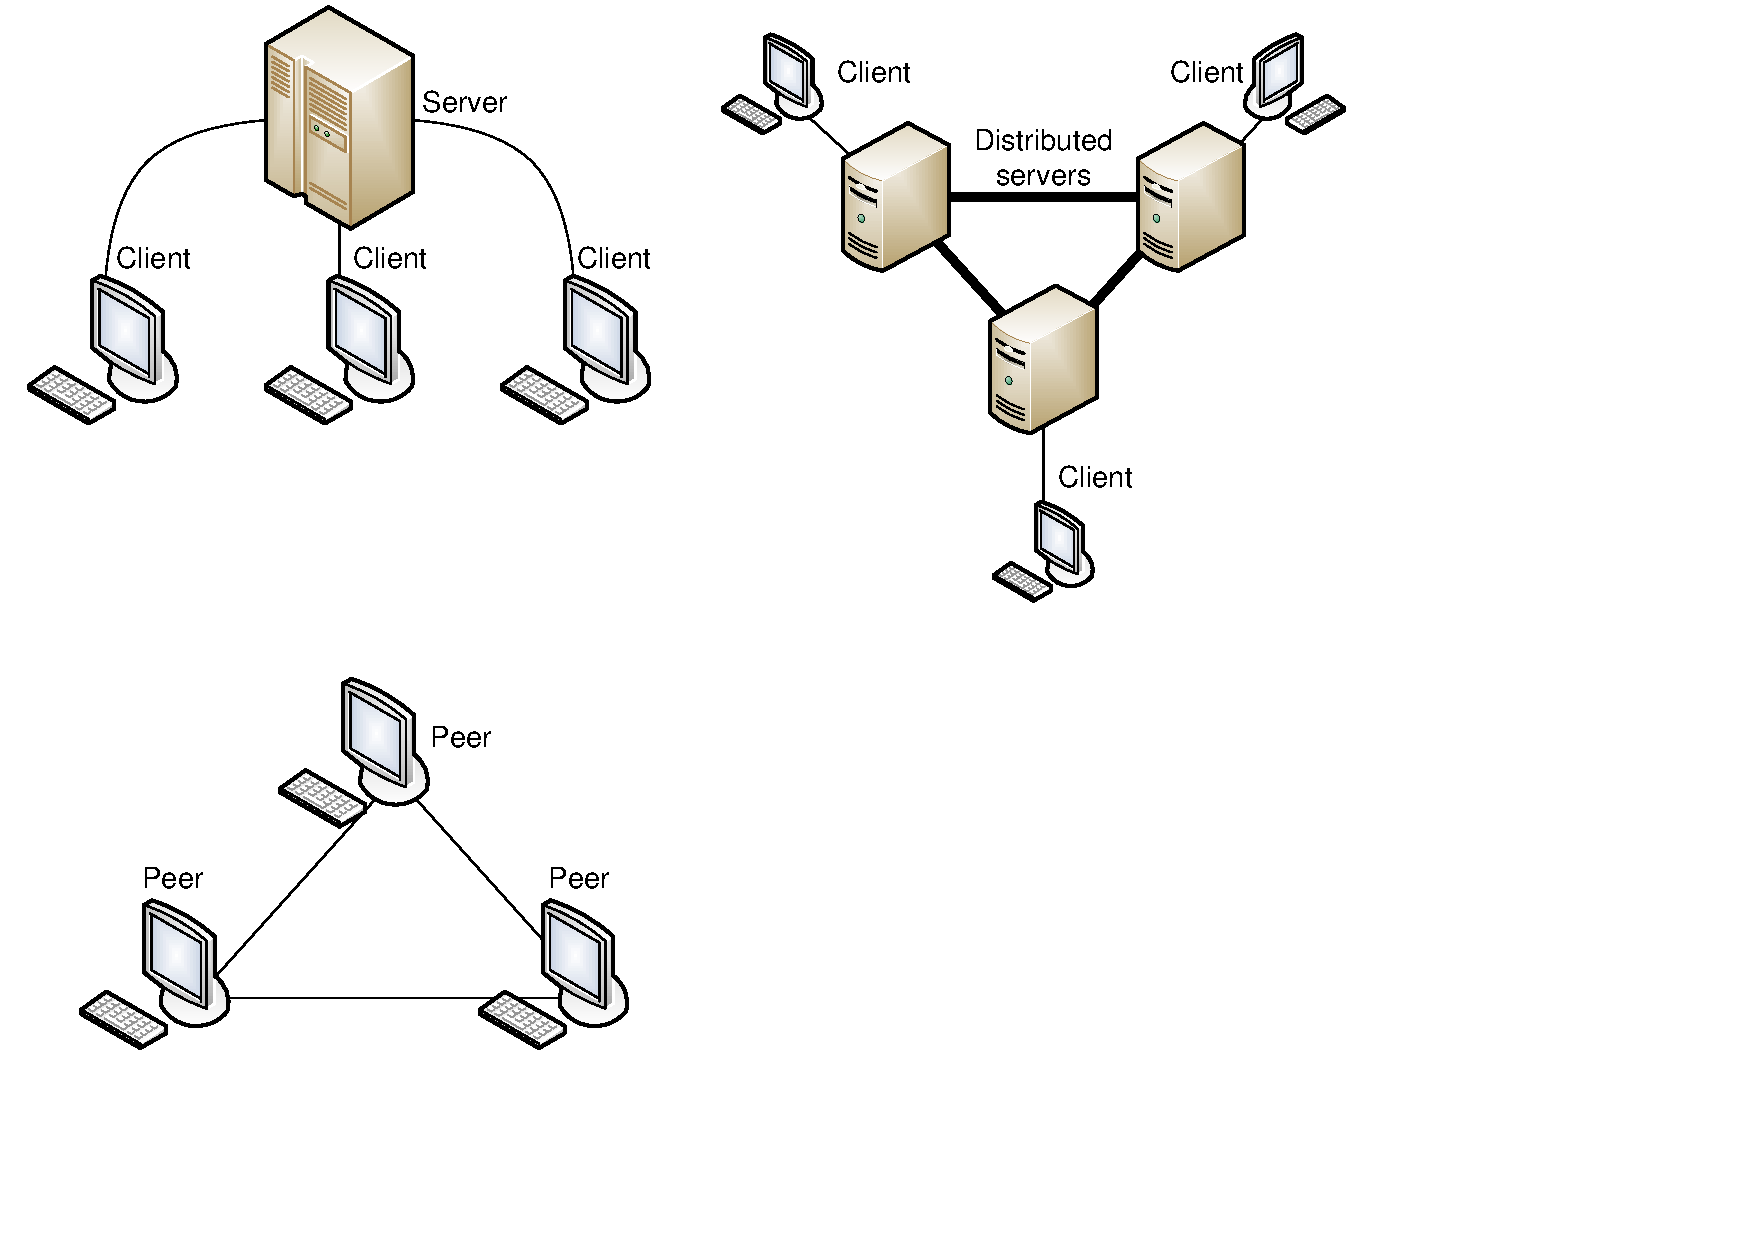
\includegraphics[clip=true, viewport= 0cm 12cm 11.5cm 21.5cm, width=0.5\columnwidth]{network_archs}}
\subfloat[Client/Multi-Server]{\label{fig_cms_arch}
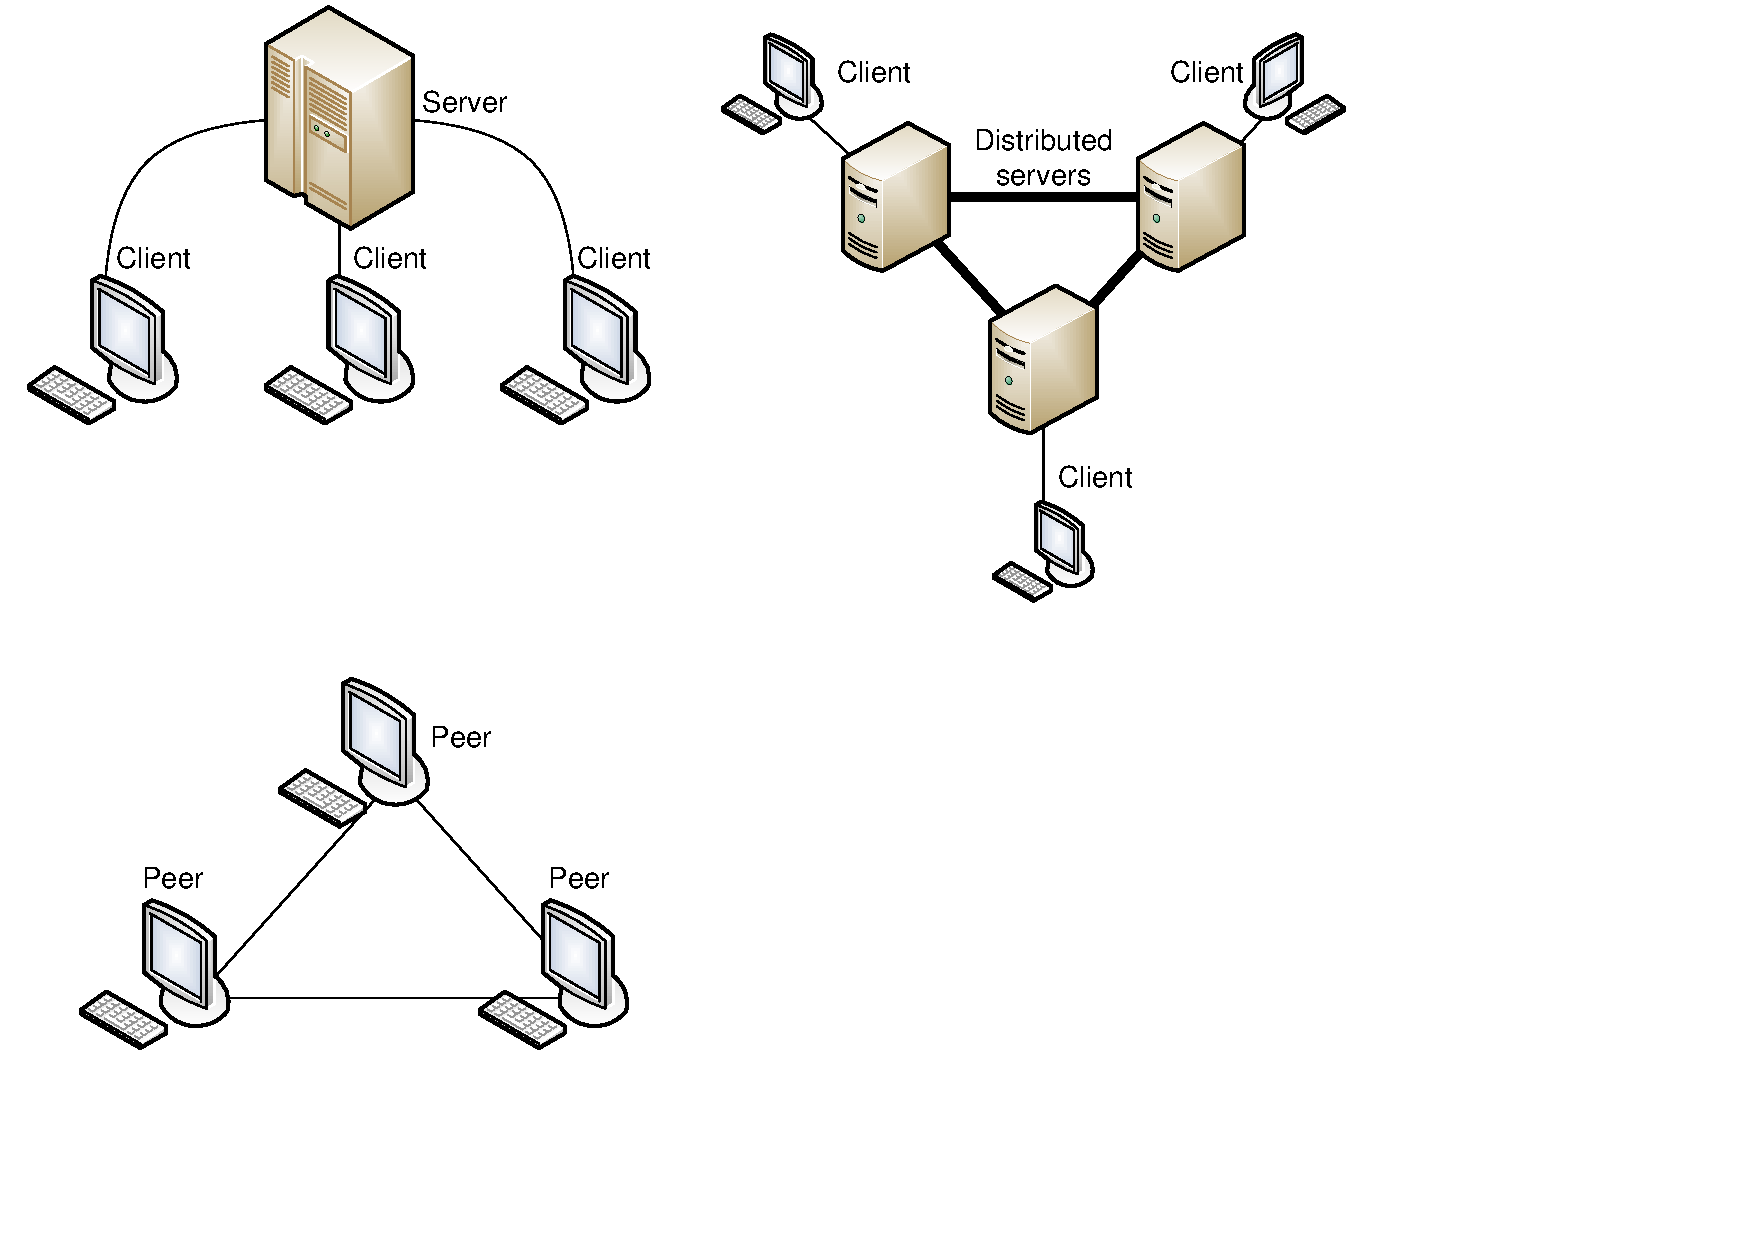
\includegraphics[clip=true, viewport= 12cm 10.5cm 23cm 21cm, width=0.5\columnwidth]{network_archs}}
\caption{Network architectures}
\end{figure}

Figure \ref{fig_cs_arch} shows the C/S model. The server is the entity on which the MMOG is hosted and is controlled by the game operator. Clients are computers operated by players, that connect to the server to play the game. The server is responsible for handling all queries from clients. Clients never communicate with other clients; they send their actions to the server and receive the updated states of other players from the server.

\subsubsection{Advantages}

The C/S architecture has two main advantages that has made it the architecture of choice for all MMOG developers. Because of the centralised approach of the architecture, both administration and security are greatly simplified. Administration is simplified, because the game operator has full control over the server, server data and code. Efficient logging is also supported, because the server is able to not only log all server actions, but also all client actions.

Security is a significant issue in MMOGs, since some players sell in-game currency for real-world currency \cite{chinese_gold_farmer}. This makes the MMOG a platform that is capable of producing income, which increases the incentive of players to gain an unfair advantage over others. The more popular an MMOG, the greater the security threat. Because the operator has full control over the server code and is never required to furnish the
client with the server code, a potential attacker never has any knowledge of the server architecture and code. Because clients are never allowed to communicate, all malicious users can be filtered out of the network by the server when detected and even banned from the network.

Operators are able to ban players, since these games usually require a game account, which is linked to a copy of the game as well as some payment method. This introduces a large cost to players whose accounts are banned. The server or cluster is also housed in a secured location, where access can be controlled. These factors simplify the security of the C/S model by allowing the developers to place all intelligence in the server.

\subsubsection{Disadvantageous}
\label{classic_cs_disadvantages}

The C/S architecture, however, does have some disadvantages. These are: weak robustness, weak scalability, high cost to the operator, high latency, high amount of required server bandwidth and weak handling of transient loads.
\begin{itemize}
\item The robustness of the system is weak because it is a single point of failure. If the server fails or goes down for maintenance, the game is off-line and players are unable to play.

\item The system is also weakly scalable, since a single server cannot easily be extended with more resources. Even if an off-line approach is used, where hardware is upgraded after the system is taken down for maintenance, the hardware required to support a game hosting more than 3000 players, become prohibitively expensive, as described in Section \ref{mmog_cost}.

The server hardware should be able to support peak system loads, which means that sufficient resources should always be provisioned to support these peak load. This is not an economically viable solution, because resources to handle peak loads are not used most of the time. This translates to operators paying for the provisioning of resources, without having active players that pay for these resources.

\item Because no clients are allowed to communicate with other clients, every change that is made to the game world by a client, first had to be communicated to the server, which in turns relays this message to all clients after applying game logic and artificial intelligence (AI) algorithms. This two hop path, with the additional time for computation added by the server as well as possible buffering at the server when many clients communicate, significantly increases the latency of the system compared to a system where direct communication is used.
\end{itemize}

\subsubsection{Client/Multi-Server}

In an effort to address some of the C/S issues, the distributed C/S, also called the Client/Multi-Server (C/MS) model, was introduced, shown in Figure \ref{fig_cms_arch}. In a C/MS model,
the server functions are distributed amongst multiple machines to distribute the server load.

In general, the issues addressed and improved by the C/MS architecture are robustness, scalability, and peak load handling. The system is more robust, because the failure of one server will not necessarily lead to the failure of the whole system for certain system designs. The system is more scalable, because many less powerful servers may be used, which allows for the hosting of more players than what is currently possible with single server hardware. It also handles transient loads better, because, for cases where loads can be predicted, resources can by moved between servers to improve the user experience.

The disadvantages of this system is that the administration complexity is greatly increased. Such systems, although capable of handling many more users than a single server, is also more expensive. These disadvantages are, however, not technical problems and so it is assumed for current games, that these systems are what is required if a game is to be hosted for a large number of players.

\subsection{The cost of doing business}
\label{mmog_cost}

With the fast growing MMOG market, many companies are spending a significant amount of money to produce premium MMOG titles. Some development cost estimates are: \$18 mil. for Aion, \$20 mil., for Everquest \cite{aion_everquest_cost}, \$63 mil. for World of Warcraft \cite{wow_cost} and \$100 mil. to \$200 mil. for Star Wars: The Old Republic \cite{star_wars_cost_1}, \cite{star_wars_cost_2}. Although these figures are purely estimates, it does show that to develop a premium MMOG title costs a lot of money.

The issue with MMOG development is that, although they cost more to develop than single player or smaller scale multiplayer games, they are just as likely to fail. Despite this, game publishers are spending a lot of money in an attempt to recreate the success that is World of Warcraft.

Because of the large revenues being generated from MMOGs, many competitors are entering the MMOG space. Currently, the rate at which new MMOGs are added to the market is outstripping the growth of the market itself \cite{newzoo_mmo_report}. Furthermore, because of the recession, over the past two or three years, game subscriptions have been shown to stabilise or even decline \cite{mmo_growth_chart}.

The significant initial investment required to develop an MMOG also doesn't present the complete picture. Another factor driving up costs for an MMOG is the money required for server hardware, maintenance and support. An MMOG is not finished when it goes live. A team of developers is required to maintain the game, release patches fixing bugs and to produce more content to keep the player base sufficiently interested to ensure that players will continue to pay \$15 per month to play. Development and maintenance costs for World of Warcraft for four years is estimated at \$100 mil. to \$200 mil. \cite{wow_cost}.

With the costs involved, it is therefore difficult for a new developer to enter into this space. After the large initial investment into the game's development, all server hardware must be acquired and staff appointed to maintain the game. This money is spent before it is known whether the game will succeed or fail. It has been estimated that during the lifetime of an MMOG, 80\% of the game revenue goes into hardware and maintenance costs \cite{cs_mmog_cost}.

\subsection{The peer-to-peer proposal}

In 2004, an architecture using the peer-to-peer networking model to host MMVEs was proposed by Knutsson et al. \cite{knutsson_p2p_first}. This
revealed a new research field, which attempts to establish the peer-to-peer (P2P) model as a viable alternative to the classic C/S and C/MS
architectures. P2P MMVE forms the focus of this work. There are various advantages to moving from C/S to P2P in MMVEs. These include: increased robustness, improved scalability, lower operator costs, improved handling of transient player load and lower latencies. The advantages are described in Section \ref{p2p_mmve_advantages} in detail,
but firstly it would be beneficial to acquire a greater understanding of the basics of the P2P network model.

\section{Peer-to-Peer systems}

A P2P network is a distributed network that exists out of many participating nodes to fulfil some objective. In this work, a P2P network is defined as being a distributed network with the following properties
\cite{Rodrigues_acm_comms_p2p}:
%
\begin{itemize}
\item \emph{High degree of decentralisation}:  No or little centralised control exists. Server functionality is distributed amongst all peers.
\item \emph{Self-organisation}: Little or no self-organisation is required in the network. Nodes are given an initial IP to allow them to join the network, but thereafter new neighbours are automatically acquired and nodes remain connected to the network, even with other nodes joining and leaving.
\item \emph{Multiple administrative domains} Peers are not under the control of any single authority. Peers in the network belong to different organisations or individuals and direct administration is impossible.
\end{itemize}

P2P systems have been popularised by mainly three systems developed in 1999: the Napster music sharing service, the Freenet data store and the SETI@home volunteer-based distributed computing project. These three projects highlighted the advantages of P2P networks being: low barrier to entry, scalability, resistance to faults and attacks, and an abundance and availability of resources.

\subsection{The OSI model and P2P overlays}

A basis of computer networking is the layered architecture model, called the open systems interconnection (OSI) model \cite{OSI_protocol_stack}. It defines various protocol layers that allow for abstraction of complex operation in the lower layers in the higher layers. The OSI layers are, from bottom to top: the physical layer, the data link layer, the network layer, the transport layer, the session layer, the presentation layer and the application layer. In practice, the session, presentation and applications layers are usually all folded into the application layer.

The physical layer is the physical transmission medium and carries physical signals. Physical level protocol standards include: IEEE 802.11 (Wi-fi), USB, Bluetooth, etc.. The data link layer, sometimes referred to as the MAC layer in the Internet protocol stack, carries frames and is responsible for point-to-point data transfer on the same local area network (LAN). Signals from the bottom layer are converted into bits and sequences of bits are grouped into frames, which is seen to be sent over the data link layer. As can be seen, every higher layer abstracts elements of the lower layer to reduce complexity.

The network layer allows communication between different LANs, using routers, gateways and host addressing. Every computer in a network is referred to as a host. A well known network layer protocol is the Internet protocol (IP), which routes all Internet traffic. The transport layer is referred to as the end-to-end layer and represents the abstract connection between a source and destination host, where all intermediate routers and LANs may be ignored, since they are abstracted away by the network layer. Well known protocols in this layer include the user datagram protocol (UDP) and transport control (TCP) protocol. Above the transport layer, for the purposes of this work, is the application layer. The application layer has access to all network services, including routing and reliable transmission.

In the C/S architecture, the client and server are both located in the application layer and communicate with each other using the transport layer. They need not be aware of any of the lower layers.

P2P networks are created and maintained in the application layer of the OSI model, called the P2P overlay. An overlay is required so peers may know which other peers are part of the P2P network, since most nodes on the Internet will not be part of the network. The overlay is then defined by the routing table information stored on each peer. The overlay can be thought of as an additional layer in the OSI model. The overlay interfaces with the transport layer and P2P applications are one layer higher and communicate by using the overlay.

Peers in an overlay network might have neighbours that have no relationship to their physical position in the underlying network.

\subsection{Structured and unstructured P2P overlays}
\label{overlays}

Overlays can broadly be classified into structured and unstructured types. The classification is mostly based on the differing methods of routing and content retrieval in the network. This section only provides a brief comparison between structured and unstructured overlays. For a detailed comparison between the two types that also deals with many of the myths of structured overlays, please refer to \cite{Castro_structured_overlay_myths}.

With unstructured approaches, one is never assured that a data item will be retrieved, even if that data item is present in the network. If many duplicates of a data item are contained in the network, this becomes less of a problem, since it is assumed that the request will be routed to some set of nodes that do  possess the item.

An unstructured architecture is well suited to content sharing and Voice over Internet Protocol (VoIP) networks, for example: P2P TV, BitTorrent, Gnutella and Skype. The reason for this is the high level of duplication in these networks, especially for popular content. It is also easier to perform keyword searches in unstructured networks and the overlay requires less maintenance.

Structured overlays have been proposed that provide for efficient routing and reliable retrieval of data items. Some of these well known overlays are: CAN \cite{CAN}, Chord \cite{chord}, Tapestry \cite{tapestry} and Pastry \cite{pastry}. The basic principle of a structured overlay is that all nodes are identified by unique identifiers (IDs).

A popular method to create the IDs is to use hashes to a circular key space, using for example, the SHA-1 hash function. Any node in the overlay network is then able to efficiently route a query with a given ID, to a node with an ID closest to the given ID. An accurate comparison is that unstructured overlays are good at finding ``hay'', while structured overlays are good at finding ``needles'' \cite{Rodrigues_acm_comms_p2p}.

\subsection{Features of structured P2P overlays}

A structured P2P overlay has certain key features that determines its lookup speed, space consumption and bandwidth requirement \cite{p2p_networking_handbook}. These features are geometries, routing algorithms, join/leave mechanisms, routing table maintenance and bootstrapping.

\subsubsection{Geometries}

An overlay's geometry determines how nodes are structured in the application layer network. The geometry allows for deterministic routing. The geometry determines the number of required lookup hops and how the network will be maintained during times when nodes join and leave the network, called churn.

\subsubsection{Routing algorithms}

The routing algorithm is directly related to the specific overlay geometry. The routing algorithm determines which nodes are traversed when a message is sent to a target node. The routing algorithm and the geometry determines the number of expected hops for a message to reach a destination.

\subsubsection{Join mechanism}

P2P networks experience constant churn, where nodes are joining and leaving the network. Mechanisms for a node to join the network should be present. This is usually in the form of a well known directory (boostrap) server. When a node wishes to join the network, the directory server sends a set of nodes that the node may want to join.

\subsubsection{Leave mechanism}

If a node leaves the overlay, its neighbours have to be informed so they may update their routing tables. This is termed \emph{routing table maintenance} and has to happen every time a peer leaves the network. Neighbouring nodes of a node that left the network might also have to inform their neighbours of the change. Two types of routing table maintenance exist: opportunistic and active maintenance.

Opportunistic maintenance attaches routing information to existing request packets. Routing data is essentially ``piggy backed'' onto existing messages. This reduced messages overhead but the rate of routing table maintenance is directly proportional to the message rate. Active maintenance makes use of explicit update messages, which required more bandwidth but is more reliable.


\subsubsection{Bootstrapping}

After having been informed of a peer to join, a joining peer may initiate the process of positioning itself in the P2P network, called bootstrapping. This is the process of finding out where the joining node fits into the overlay in terms of the geometry. If the overlay requires that all nodes be connected in a ring organised by ID, then the joining peer must discover the nodes whose IDs are one more and one less than its own and join those two peers.

The process of bootstrapping is complete when a joining peer becomes a functioning member of the P2P overlay.

%TODO: Add something about the effect of the hashing and why it's important

\subsection{Advantages}

\begin{itemize}
\item P2P networks have a low barrier to entry, since little or no centralised infrastructure is required to maintain the system. This makes P2P networks inexpensive to operate and is one of the reasons Napster was able to provide its service for free.

\item P2P networks are considered scalable. Pure P2P networks can theoretically grow from hundreds to millions of nodes, with the service remaining functional. This is all possible without the need for the operator to acquire more infrastructure, as opposed to the centralised client/server network, which required more powerful server clusters are the network grows to handle the growing number of client requests.

\item A P2P network is also resistant to faults and attacks, since the failure of a single node has little to no effect on the network. This is because there are usually few nodes that are critical to the correct functionality of the system. To incapacitate a P2P network, an attacker usually has to shut down a large proportion of the network.

\item Not only does a P2P operator not require its own infrastructure, but the P2P infrastructure that forms part of the network and consists of peer machines provide abundant and highly available resources, being computation power, long term and short term storage. This means that P2P networks can be designed to run on powerful computers.
\end{itemize}


\section{Peer-to-Peer MMVE network architectures}
\label{p2p_network_architectures}

P2P MMOGs are considered a sub-class of P2P Massively Multi-user Virtual Environments (MMVEs), a class that also includes large scale military simulators.

This architecture does, however, still have a few major issues that need to be solved before MMVEs can be developed that use it. If
these issues, discussed in Section \ref{key_challenges}, can be solved, a P2P architecture holds some powerful advantages over a C/S system.

The core idea of the P2P model is that each peer contributes sufficient resources to the network to host itself. This also means that all functions of the server in the classic C/S model are distributed amongst all peers.

\subsection{Advantages}
\label{p2p_mmve_advantages}

\begin{itemize}
\item The P2P architecture is robust, because there is no server that can fail, only individual peers. Individual peers failing will not affect any other peers other than the peer that failed. This behaviour makes game down-time extremely unlikely.

\item The system is scalable, because every peer hosts itself.

\item Because of the high scalability, no extra resources are required from an operator perspective, when more peers join the network.

\item P2P networks also efficiently handle transient loads, since the joining peers contribute their own resources. If many players suddenly enter the
game no resource provisioning issues will arise, since peers already possess the required resources.

\item P2P architectures create a lot of opportunities for independent developers, because a large initial investment is no longer required to purchase
the expensive server hardware. Not only are hardware costs reduced, but running costs are also reduced.

\item Bandwidth required by the game server is now shared amongst users, which means that very little bandwidth costs will be incurred by the provider.

\item Latency is improved, because it is now possible to directly communicate between peers and it is not necessary to communicate via a server.
The distribution of the load as well as direct communication will further reduce latency.
\end{itemize}

\subsection{Requirements}

Key requirements have been identified for the creation of a P2P MMVE. What follows is an expansion and reinterpretation of the requirements identified by Schiele et al. \cite{Schiele_p2p_requirements}.

\subsubsection{Distributed computation}
\ref{distributed_computation_requirement}

Non-Player Characters (NPCs) are characters that are not controlled by any human player, but are rather controlled by some artificial intelligence routine or script executing on some host machine. These characters represent the traders and monsters in MMVEs and usually contain sets of rules that determine how they should interact with Player Characters (PCs) as well as their own state information. An NPC's state can be how much money and items it has to trade or how much health it still has after being attacked by a player.

Some game objects require computational power to function. An example of this is the Artificial Intelligence routines of NPCs or the computation of physics effects on in-game objects. In P2P MMVE, it might be required to distribute these computational tasks to offload computation load from peers that do not have sufficient resources.

\subsubsection{Consistency}
A key challenge with any networked game is how to maintain state consistency between users in the virtual world. In other words, to ensure that all users perceive a virtual world in the same state. Solving the state consistency problem for P2P MMVEs is one of the major development challenges and forms the focus of this work. The challenge of state consistency will be described in detail in Chapter \ref{chp:CONSISTENCY}.

\subsubsection{Persistency and state management}

\subsubsection{Self-organisation}\
Handling of user churn

\subsubsection{Availability}
Game must always be online (P2P requirement)

\subsubsection{Interactivity}
Low latency interaction and masking latency with dead reckoning

\subsubsection{Scalability}
Server and peer bandwidth requirements

\subsubsection{Security}

Security, which includes cheating mitigation, has been identified as a major issue for P2P networks \cite{knutsson_p2p_first}, \cite{challenges_p2p_gaming}, \cite{cheat_proof_event_ordering}. The challenges reside in the fact that peers are not under the control of the game producer. Since all server data are distributed amongst peers, all peers have access to sections of the server data. Peers also have access to the distributed server code. One advantage that can be exploited to prevent cheating is that no peer contains all server data and no single peer has more authority than another.

\subsubsection{Efficiency}
The peer must efficiently implement the server, since it still has to be a client as well

\subsubsection{Maintainability}

\subsubsection{Incentives}

P2P schemes require all players to share resources in order to ensure correct functionality. Players might, however, not want to share their resources, whilst still benefiting from the resources of others. The purpose of incentive mechanisms is to ensure that all players contribute resources, by incentivised contribution.

All distributed resource sharing models require incentive mechanisms. For example, Bittorrent systems use the tit-for-tat protocol to ensure that all people downloading data are also contributing data \cite{tit_for_tat}. Such mechanisms are also required with P2P MMVEs. One advantage in designing an incentive mechanism for a P2P MMVE is that players can be made to contribute resources for the duration of play. The issues with file sharing systems are not present where a peer, after downloading a file, has no more incentive to contribute.

\subsubsection{Structured P2P overlay}

Because there is no assurance that a data item might be retrieved from an unstructured network, especially when that item is scarce, unstructured overlays are not considered adequate as a basis for P2P MMVEs, where all data items must be available at all times.

A P2P MMVE architecture requires a structured P2P overlay in the broad sense. In P2P MMVEs, peers have to be connected in some geometry and it should be possible to route messages between peers. P2P MMVEs require a bootstrapping server to enable peers to join the network and be placed in it. A P2P MMVE architecture should handle churn with a minor impact on system operation. Most importantly, all objects stored in the P2P MMVE should be available at all times.

\subsection{Key challenges}
\label{key_challenges}

Using P2P MMVEs has many advantages, some challenges still remain. The main challenges are state consistency, limited peer bandwidth, cheating mitigation, incentive mechanisms and distributed computation. This section will present some information on work that has been done in the different areas and talk about the maturity of the various solutions. In general though, most solutions are still research projects and none have yet been implemented as commercial products.

\subsubsection{Peer bandwidth}

In a paper by Miller and Crowcroft, a packet simulator was created to determine the required bandwidth and effective latency, if a game such as World of Warcraft were to be implemented using P2P technologies \cite{Miller_p2p_infeasability}. Their simulation results indicate that today's networks are not able to host P2P MMVEs, with the required bandwidth and latency constraints. Such a significant result requires verification, but at the least, it shows that reducing bandwidth and latencies for P2P MMVEs should be a primary design requirement.

\subsubsection{Cheating mitigation}
\label{key_challenges_cheating}

%Describe "server data" in terms of a more generic form to be able to have that generic form in the server and p2p architecture.

There are various security issues that are usually classified according to the level in the OSI protocol stack where they occur. The areas identified by \cite{cheat_proof_event_ordering} and expanded upon by \cite{cheating_taxonomy} are: game level, application level, protocol level and infrastructure level. The description is consistent with the generally used layered security model \cite{distributed_systems_security}.

\begin{itemize}
\item Game level cheats are ways in which a malicious player may gain an unfair advantage over other players, within the confines of the game. These cheats are usually because of software bugs and some examples are duplication and teleport cheats.

\item Application level cheats are where malicious players alter the game software to gain an unfair advantage. This is usually done by gaining access to the game state to which they should not have access at the current time. An example of this is ``map reveal'' cheats in strategy games, where the ``fog of war'' is removed and the player can observe all the opponent's movements. Other cheats that are used include augmenting the player's UI with extra information that allows the player to make more informed decisions.

\item Protocol level cheats are cheats based on the different methods of communicating data across the system. These usually concern dropping, delaying of modifying IP packets to achieve certain outcomes in the game.

\item Infrastructure level cheats concern exploiting the underlying infrastructure on which a game is built. Types of infrastructure cheats include denial of service (DOS) attacks on the P2P overlay to prevent messages that should be forwarded by a peer from being forwarded.
\end{itemize}

As with all taxonomies, all cheats may not cleanly fit into one if these boxes, some cheats may occur over multiple levels or a cheat with a specific outcome can be implemented differently on different levels. The field of P2P security has recently received more attention than in the past and has started to bear fruit \cite{survey_p2p_game_cheats}.

This is, however, an ongoing research field with many issues still open. For an in-depth review of the security issues facing peer-to-peer system in general, refer to \cite{p2p_security_issues}. These issues are the same issues facing P2P MMVEs, with the exception of the game and application layer issues.

\subsubsection{Incentive mechanisms}

Some proposed incentive schemes increase a player's reputation when resources are provided  \cite{classic_p2p_reputation} \cite{proactive_reputation}. This might create a type of meta game, where players try to gain as much reputation as possible. It can however be argued that this scheme does not really enforce the provisioning of resources. A player who does not want to provide resources might not see a higher reputation as sufficient incentive to provide resources.

Other issues with incentive schemes is that sometimes players might have insufficient resources. Such players should be aided by other players with sufficient resources and not be disallowed from playing the game. When limited resources are taken into account, the issue of reporting a false amount of available resources becomes a problem. A peer that has sufficient resources, might report insufficient resources, to avoid being penalised. It is evident that there is a need for more research in this field.

\subsubsection{Distributed computation}

Some architectures assume that the computational requirements will be fulfilled where the object state is hosted \cite{solipsis}, but other schemes exist that allow for the CPU power to be distributed amongst peers. One such scheme makes use of a ``job board'' like mechanism, where tasks are advertised on specialised peers. All peers monitor these specialised peers and may elect to perform the advertised tasks \cite{fan_mediator_paper}.

\subsubsection{State consistency}

The state of the art of state consistency techniques will be reviewed in detail in Chapters \ref{chp:CONSISTENCY} and \ref{p2p_MMVE_state_persistency}.

\section{Research objectives}

\section{Related work}

\section{Contributions}
\label{objectives}

\begin{itemize}
\item A generic state consistency model is developed that encompasses both C/S and P2P consistency models.

\item A review of various state management and state persistency systems is performed.
    \begin{itemize}
    \item The state management survey identifies some key metrics by which state management systems may be compared.
    \end{itemize}

\item A novel state management and persistency architecture, called Pithos, is proposed and implemented in simulation, which increases reliability and responsiveness compared to classic state persistency methods.
    \begin{itemize}
    \item Multiple methods of implementation are described that provide different benefits, depending on the situation.
    \item The various implementation methods are evaluated and recommendations are made on which methods work better in which situations.
    \end{itemize}

\item A statistical model for expected object lifetimes is developed and used to verify the Pithos results.
\end{itemize}

\begin{itemize}
\item Early in the literature study phase, it was discovered that no research projects that deal with P2P MMVEs present the complete picture of the field. A significant amount of research has been done in the field of state consistency (reviewed in Chapter \ref{chp:CONSISTENCY}), but in this field, no model has been provided which shows what is required to build a complete state consistency architecture. The first contribution of this work is to provide such an architecture at the start of Chapter \ref{chp:CONSISTENCY}.

\item The generic consistency model that is developed is not only applicable to P2P MMVEs, but to any networked virtual environment that required state consistency. The generic consistency model is also compared with well known client/server and P2P consistency models, to show how the existing models can be seen as more specialised versions of the generic consistency model.

\item After developing a generic consistency model, this work then focusses on an area of state consistency that has received little attention from the research community, namely: state management and state persistency. This area is concerned with managing object states as they are updated by events occurring in the virtual environment. Also during a literature review of this field, it was found that no thorough review of this field has been done to compare the different types of storage systems present in P2P MMVEs and presented in the literature. We then preceded to perform such a review, presented in Chapter \ref{p2p_MMVE_state_persistency}. The results of this survey has also been published in the IEEE Transactions of Parallel and Distributed Systems \cite{gilmore_p2p_mmog_state_persistency}.

\item During the survey, some key metrics were identified by which state management and state persistency systems may be described. A proposal was also made as to how these metrics may be measured. What was found upon completion of the survey is that no storage system has thus far been created to satisfy all identified metrics. Work was then undertaken to develop a novel state management and persistency architecture that satisfies all identified requirements.

\item The state management and persistency architecture has been developed and called ``Pithos''. Pithos has been implemented in a network simulation framework, called Oversim, which runs on the Omnet++ simulation environment. The Oversim framework itself has also been extended to implement our novel generic consistency architecture. Pithos has been implemented in the root object store section of this architecture.

\item Many of the key mechanisms in Pithos, such as object retrieval, have been implemented using multiple methods. These methods are then compared to determine the advantages and disadvantages of each. Pithos is also compared to the storage systems identified. Pithos always shows similar or improved performance over classic storage systems in all identified areas.

\item In order to verify the correct functioning of Pithos, mathematical models are also developed to describe Pithos's performance in the various identified metrics. Amongst these is a novel Mathematical model that makes use of an embedded continuous time Markov chain to determine expected object lifetime for varying amounts of network churn, various network sizes and replication rate. The mathematical model is compared with actual Pithos results and appears to match almost exactly.
\end{itemize}

\section{Summary of this work}

Chapter \ref{chp:CONSISTENCY} presents an overview of state consistency models. Initially, it describes the general process by which state consistency is achieved. Some classic consistency models are then presented in terms of the generic model. Consistency models for P2P MMVEs are then presented, with an overview of work that has been done in each of the various sections required to implement a complete consistency model.

Chapter \ref{p2p_MMVE_state_persistency} focuses on the state management and state persistency aspect of P2P MMVE state consistency. Initially, some metrics are defined according to which different storage architecture may be compared. A literature review is then presented, where papers that deal with various storage techniques are grouped and the advantages and disadvantages of each group is then discussed. This chapter also identifies a need for a novel state management and persistency architecture.

Chapter \ref{chp:DESIGN} describes the design and implementation of Pithos, the novel state management and persistency architecture. Initially, the overarching Pithos design is described, including the perceived use case and design goals. The Oversim simulation environment is then described, along with the extensions that were made to model the generic consistency model. The Pithos implementation is then described in terms of Oversim modules. Key mechanisms that implement that Pithos design are then presented with reference to the Pithos Oversim modules. Various methods to implement some mechanisms are descried.

Chapter \ref{chp:EVALUATION} evaluates the Pithos implementation. The performance of the key mechanisms are presented and the various implementation methods are compared. Pithos is also compared with other storage implementations.

Chapter \ref{chp:MODELLING} models Pithos's performance with reference to the identified metrics for P2P MMVE storage systems. A focus is placed on expected object lifetime and a novel model is developed, based on an embedded continuous time Markov chain.

Chapter \ref{chp:VERIFICATION} compares model results with Pithos simulation results. The purpose of this chapter is to verify the correct functionality of Pithos, according to mathematical models. The chapter also explores how to design storage systems with desired object lifetimes.

Chapter \ref{chp:CONC} concludes the work. It presents a summary of the work, lists contributions made and discusses some future areas of research.

\chapter{State Consistency}
\label{chp:CONSISTENCY}

A recent article has identified six key challenges of P2P networks: Interest Management, Game Event Dissemination, Non-player Character (NPC) Host
Allocation, Game State Persistency, Cheating Mitigation and Incentive Mechanisms \cite{Fan_deisgn_issues_p2p}. A brief overview of these challenges
will be introduced below.

\begin{figure}[htbp]
 \centering
 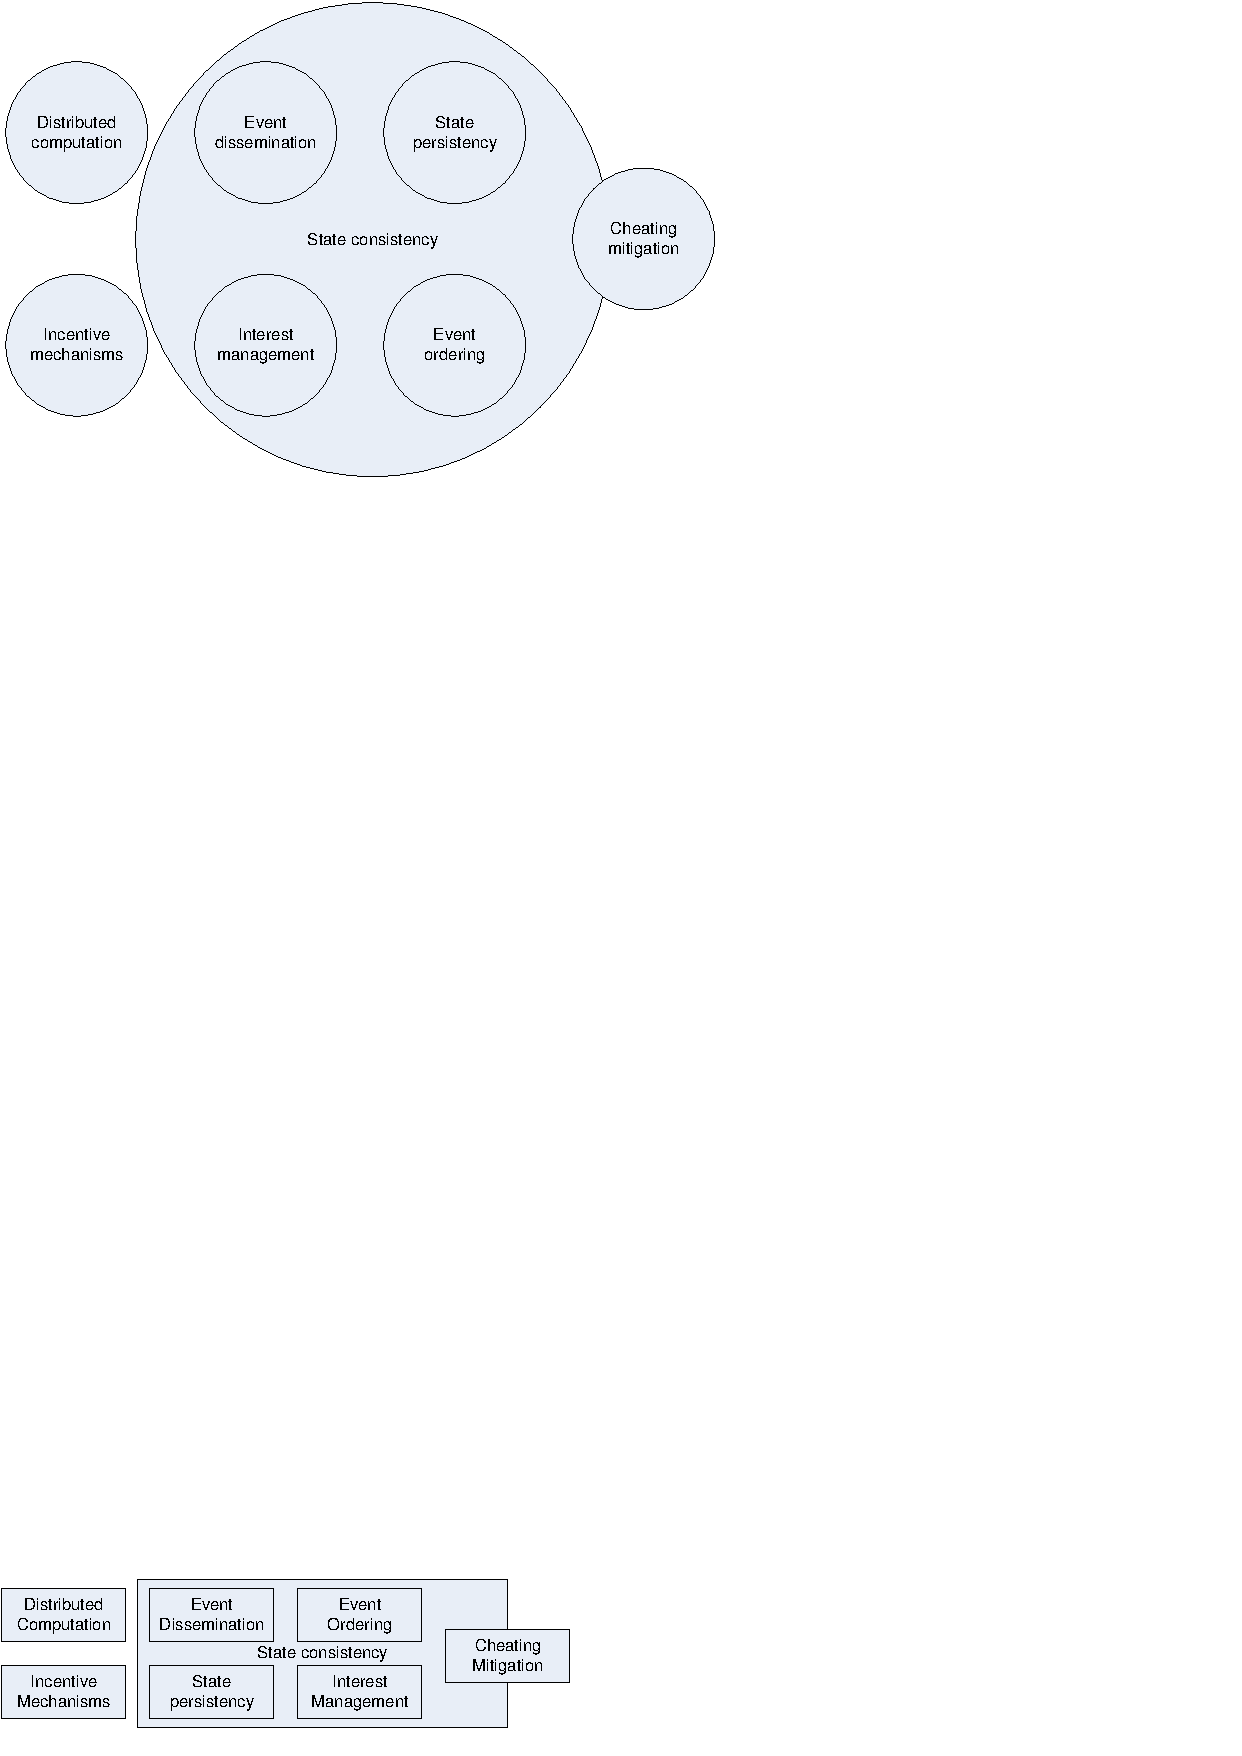
\includegraphics[clip=true, viewport=0cm 0cm 10cm 3cm, width=0.5\columnwidth]{Component_VEN}
 \caption{VEN diagram showing the relationship between different characteristics}
 \label{fig_component_ven}
\end{figure}
%
As shown in Figure \ref{fig_component_ven}, of the six challenges mentioned, Interest Management, Game Event Dissemination and Game State Persistency
all form part of State Consistency, with some aspects of Cheating Mitigation also a part of State Consistency. Also part of state consistency is
event ordering, which deals with how to ensure that the system remains causal \cite{GauthierDickey_low_latency_event_ordering}.

Key to designing an MMVE is to design its state consistency architecture. On a physical level, each computer that executes a virtual environment (VE) is executing a copy of the virtual environment. This is because a computer can only operate on what is stored in its primary memory. Because computers cannot access each other's primary memory banks, the necessity of multiple object copies is created.

A virtual environment can be characterised by its state. The \emph{environment state} (\emph{game state} when the environment is an online game) includes all positions, health and other attributes of all avatars, NPCs and other objects in the VE. The environment state consists of a collection of objects. An NPC as well as an immutable plant are both examples of objects that together make up the environment state.

When discussing how to segment VE state, it is sometimes easier to speak in terms of \emph{objects}, since they are separable. For the purposes of this work, objects are entities with both state and logic, which means they consume both storage space, as well as computing resources. Objects can also produce events, which should be sent to other objects. When this definition is used, NPC objects may be classified as a specific type of object, which forms part of the global game state.

The existence of multiple object copies necessitates an object consistency model. In MMVEs, each computer uses the information of the virtual environment, stored in memory, to display the virtual environment to the user. The user makes decisions based on what is displayed and the executed operations on the environment. These operations can effect change in the environment and this change has to be communicated to all other entities capable of interacting with the environment. The fact that users operate on a local version of the environment and that the environment should appear the same to all users requires state consistency mechanisms.

\section{Event-logic-update cycle}
\label{event_logic_update}

It is however impossible for multiple object states to always be consistent, because it takes time to send a message about an object update that has occurred. It is, therefore, not a good design to allow objects to be locally changed and those changes to then be communicated to other objects, because other objects may also have been locally changed in a way that would not allow for the change in the first object.

An example would be of one player in a virtual game world dealing five damage to another player with five health. When the damage is dealt, the target player is killed. If, however, the player drank a potion that gives it some health, the damage dealt by the first player would not kill him. The state of the player being dead and the player being alive is not possible at the same time.

To overcome this difficulty, a disconnect is introduced between the actions that can be performed on objects and the effect that the actions can have on objects. This is called the event-logic-update cycle \cite{}.

\emph{Events} are generated by objects and can be thought of as actions taken by agents, where agents can be humans or artificial intelligence (AI) scripts. These include casting a spell, using an item or walking.

\emph{Environment logic} is applied to events to determine what updates should be applied to the environment state. Environment logic is thus a ``think'' function, which determines how the environment should change as a result of an event. Another way to think about environment logic is to see it as the game rules.

A player casting a spell might cause another player's health to be reduced, her own health to be increased or a monster to spawn. When a player is walking, the logic will cause the player's position to update at the player's walking speed.

Environment logic communicates how the world should change via \emph{state updates}. State updates are the incremental changes that specify how the environment state should change.

An object exists in two forms: the authoritative object and the non-authoritative object. The state of the authoritative object is considered to be the true state or absolute state. Copies of the authoritative object can be made, but these copies are all non-authoritative objects. If a discrepancy occurs between an authoritative object and a non-authoritative object, the state of the authoritative object is considered to be the true state. The work of the consistency mechanism in the VE is to ensure that all non-authoritative object states follows the authoritative object state within a time frame that is reasonable for the particular VE and the particular type of object.

Authoritative objects are the objects traditionally housed on the server in the C/S based MMVEs. All clients obtain replicas of these objects and duplicate them locally in order to perform low latency computations. An example would be an NPC monster. When players perceive the monster in the virtual world, a duplicate of the NPC objects is sent to the user's computer for display purposes. When another player attacks the NPC, the change in health will be computed at the server and an update is then sent in order to ensure consistency between root and replica objects.

\subsection{General flow}
\label{general_flow}

\begin{figure}[htbp]
 \centering
 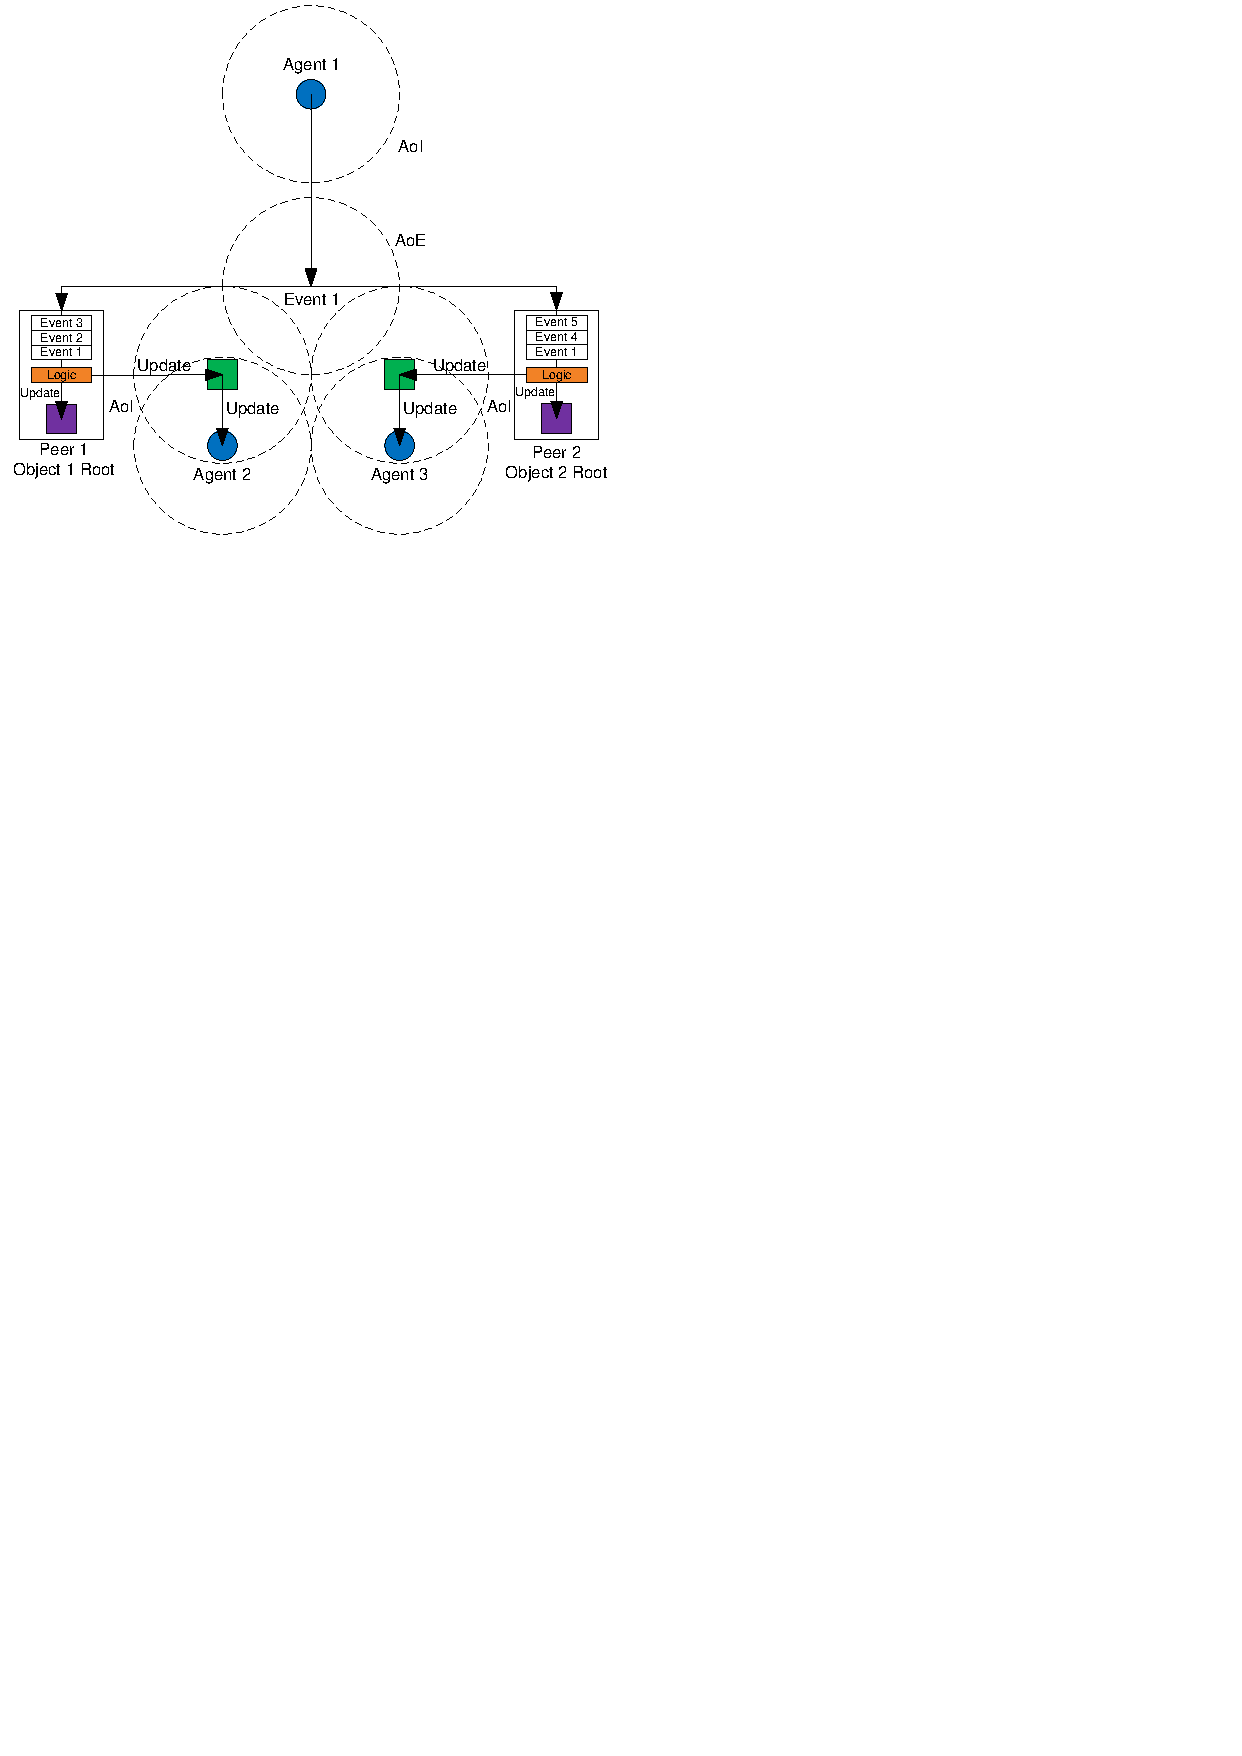
\includegraphics[clip=true, viewport=18mm 227mm 69mmm 292mm, width=0.6\textwidth]{generic_consistency_graphic}
 \caption{Graphic showing the flow of events and updates to achieve state consistency}
 \label{fig_event_update_flow_graphic}
\end{figure}

Figure \ref{fig_event_update_flow_graphic} depicts the flow of events and updates in response to the generation of an event by some agent. Agents are defined to be some form of intelligence that can interact with the virtual environment.

In Figure \ref{fig_event_update_flow_graphic}, Agent 1 generates Event 1 at the remote location shown. To maintain generality, events are defined to possess areas of effect (AoEs). An event's AoE determines which objects are in range to be potentially affected by an event. When an event's AoE encloses an object, that object is in range to be affected by the event. Whether the object is affected by the event, will be determined by the game logic.

In Figure \ref{fig_event_update_flow_graphic}, Event 1 affect Object 1. Event 1 is, therefore, sent to Object 1's root node, i.e. the peer housing the authoritative copy of Object 1. Determining which objects are affected by an event is termed \emph{event layer interest management}. Delivering the event to the root nodes of the affected object is termed \emph{event dissemination}.

When Event 1 arrives at Peer 1, containing Object 1, the event is placed in a event queue in an order based on the time each event occurred. The process of determining which order events have to be processed in is called \emph{event ordering}. Many events will be arriving at an object's root node from multiple agents simultaneously.

After event ordering has been performed, environment logic is applied to determine hoe a specific event will affect a specific object. To determine possible updates, that state of other objects might also have to be taken into account. An example is firing at a player through a wall. If the thickness of the wall determines how much damage is delivered to the player, the root node processing the damage to the player object will have to know the thickness of the wall.

When an event has been translated into a state update, the root object on the root node is updated. The new state of the object should also be communicated with all agents that can perceive the object in the virtual world. An object is perceived by an agent if the agent's area of interest (AoI) encompasses the object. Determining which agents should receive objext state updates is termed \emph{update layer interest management}. In the figure, Object 1 is perceived by Agent 2. Peer 1 therefore has to send an update to the peer housing agent 2. Delivering state updates to the affected agent peers is termed \emph{update dissemination}.

When the update is delivered to Agent 2, the local object state is updated and the object's new state is displayed to the agent to allow the agent to make decisions and, therefore, generate events based on the new object state.

\subsection{Generic event-update model}
\label{generic_event_update_model}

During the literature review process, many papers were reviewed that were said to deal with state consistency in P2P MMVEs \cite{}. These papers that were said to contain novel state consistency methods for P2P MMVEs, always only pertained to a specific part of the state consistency model and compared other papers related to the same part. All these papers improved on the various modules that make up a state consistency model, but failed to provide an overview of the bigger picture and how to place the work in the paper in the framework of a state consistency model.

Reviewing the various papers, it became evident that a higher level state consistency model is required to place all the work done in this field into perspective.

\begin{figure}[htbp]
 \centering
 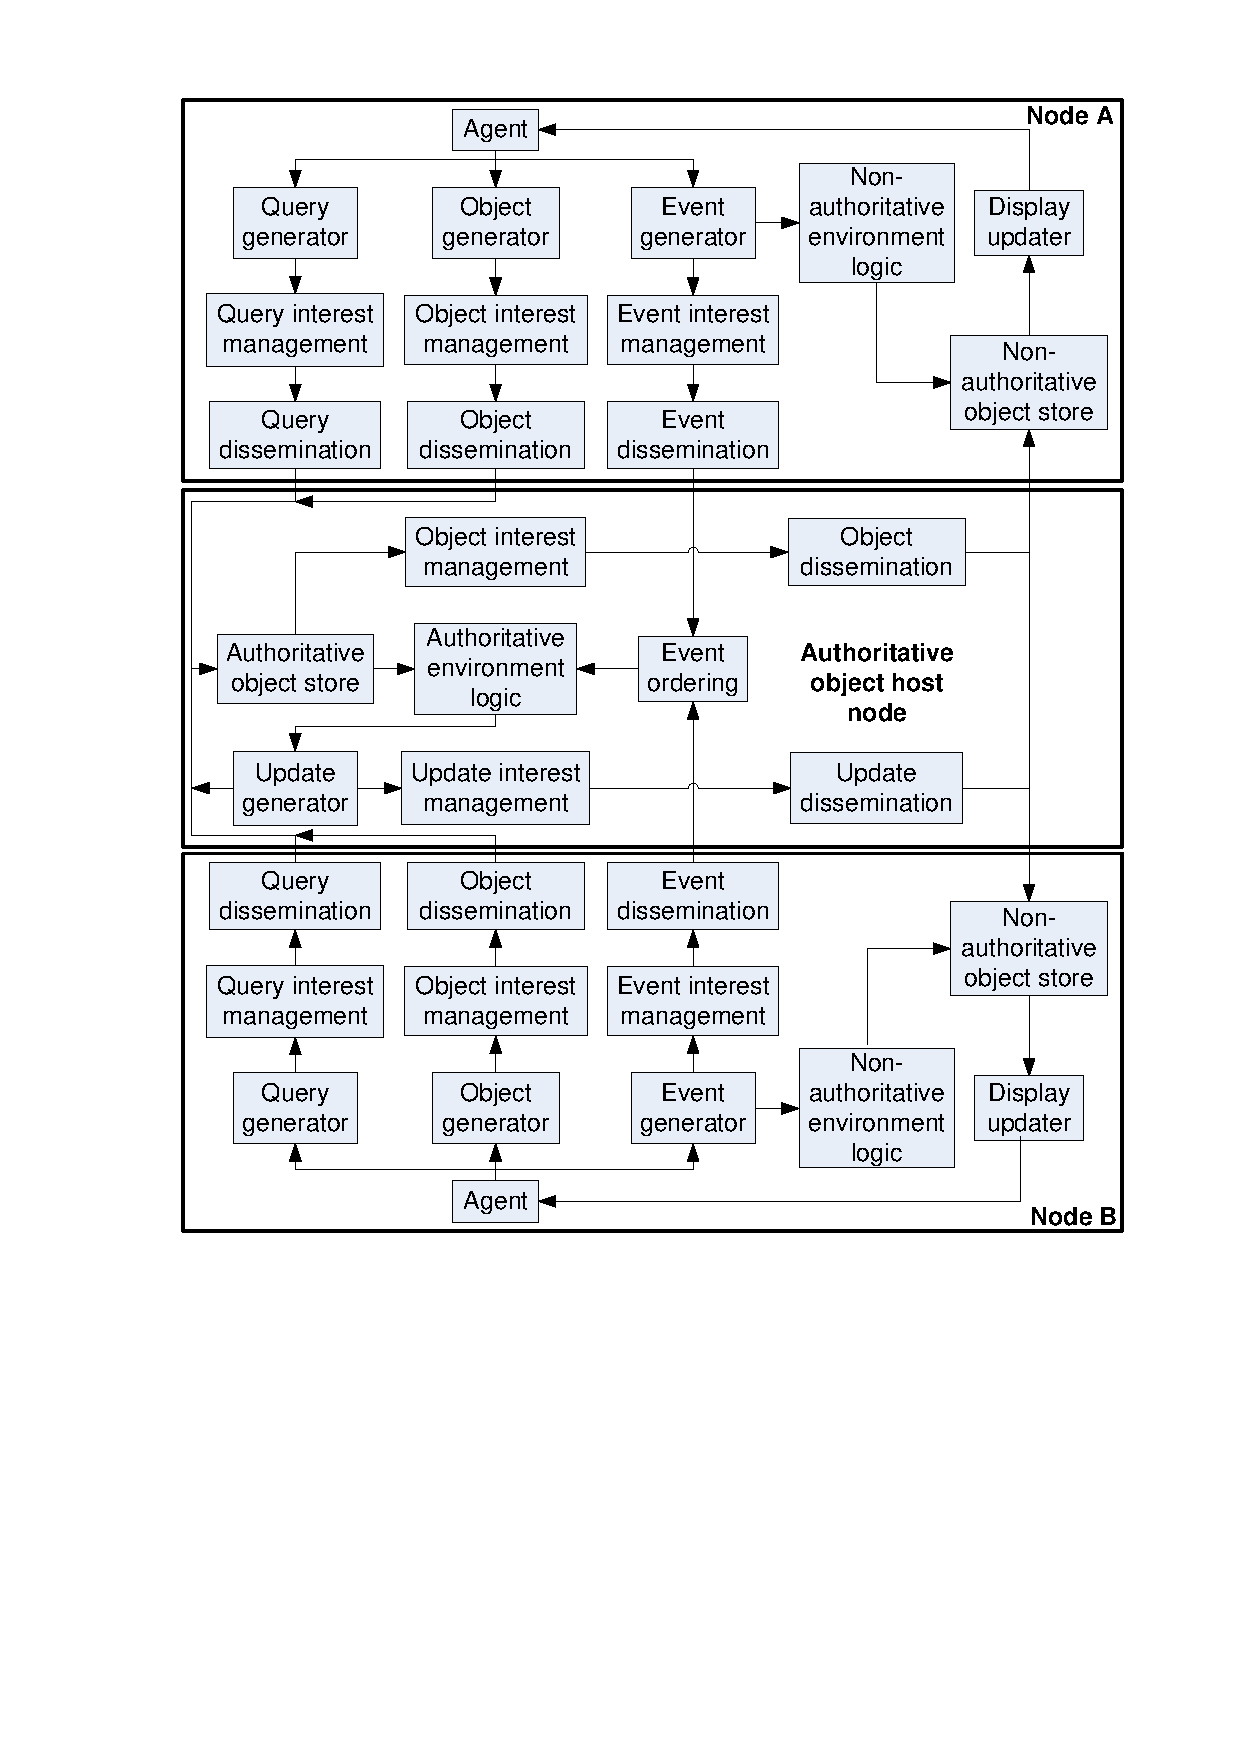
\includegraphics[clip=true, viewport=49mm 82mm 156mm 288mm, width=0.6\textwidth]{generic_consistency_flowdiagram}
 \caption{Flow diagram describing the event-update flow cycle and all steps required, from generating an event to delivering an update, to ensure object consistency.}
 \label{fig_event_update_flowdiagram}
\end{figure}

Figure \ref{fig_event_update_flowdiagram} shows the generic consistency flow diagram to ensure object state consistency. The agent, introduced in Section \ref{general_flow} is a player or AI script. An agent views the game world as the game displays is, makes some decisions on how it would like to influence the game world and then takes some action. The action of an agent is translated into an event.

Event layer interest management determines which objects will be affected and on which nodes these objects are housed. Event dissemination deals with how information is sent to peers after interest management determines which information should be sent. The first application of event dissemination for online games can be found in \cite{first_GED}.

The game logic is then applied to each received event and a corresponding update is generated. It is possible that the future state of an object might depend on the current state of the object, the received event and the state of some other object. The game logic might, therefore, require the states of other authoritative objects.

Storing authoritative data requires state management and state persistency. State management is the storage of objects in primary storage, while state persistency is the storage of the VE on secondary storage. State persistency does not have such rigorous responsiveness requirements as state management, as described in Section \ref{char_responsiveness}.

After the combination of event, object states and game logic, an event is generated. Update layer interest management determines which nodes require this update. These will typically be the nodes whose agents can perceive the object in the virtual environment and, therefore, stores local copies of the object.

Update dissemination will deliver the update to all local copies of the object. Multiple object updates may be generated for a single event. Any generated update may have to be delivered to multiple nodes that contain local copies of the object.

The flow diagram in Figure \ref{fig_event_update_flowdiagram} shows all actions that should be taken to ensure object consistency. This model is applicable to all known state consistency models for C/S as well as P2P network architectures.

What changes for the various architectures is where the root object is housed, and how the hosts of the root object are distributed. In a C/S system, all root objects are housed in the server. In a P2P architecture, root objects can be distributed on a number of peers or super peers, depending on the specific architecture. The various state consistency schemes for both C/S and P2P networks will be reviewed in the next sections.

\section{Classic consistency models}
\label{classic_models}

An overview of the two common models, currently used in computer games will be described. The models used in P2P MMVEs are all permutations of these two basic models. The two models are based on the two different network models. These are the fully distributed model, also called the event-based model \cite{p2p_cm_aoe}, and the C/S-based model, also called update-based model
\cite{unreal_networking}.

\subsection{Event-based (Fully distributed)}
\label{classic_event_based}

\begin{figure}[htbp]
\centering \subfloat[Event-based (fully distributed)]{\label{fig_p2p_cm}
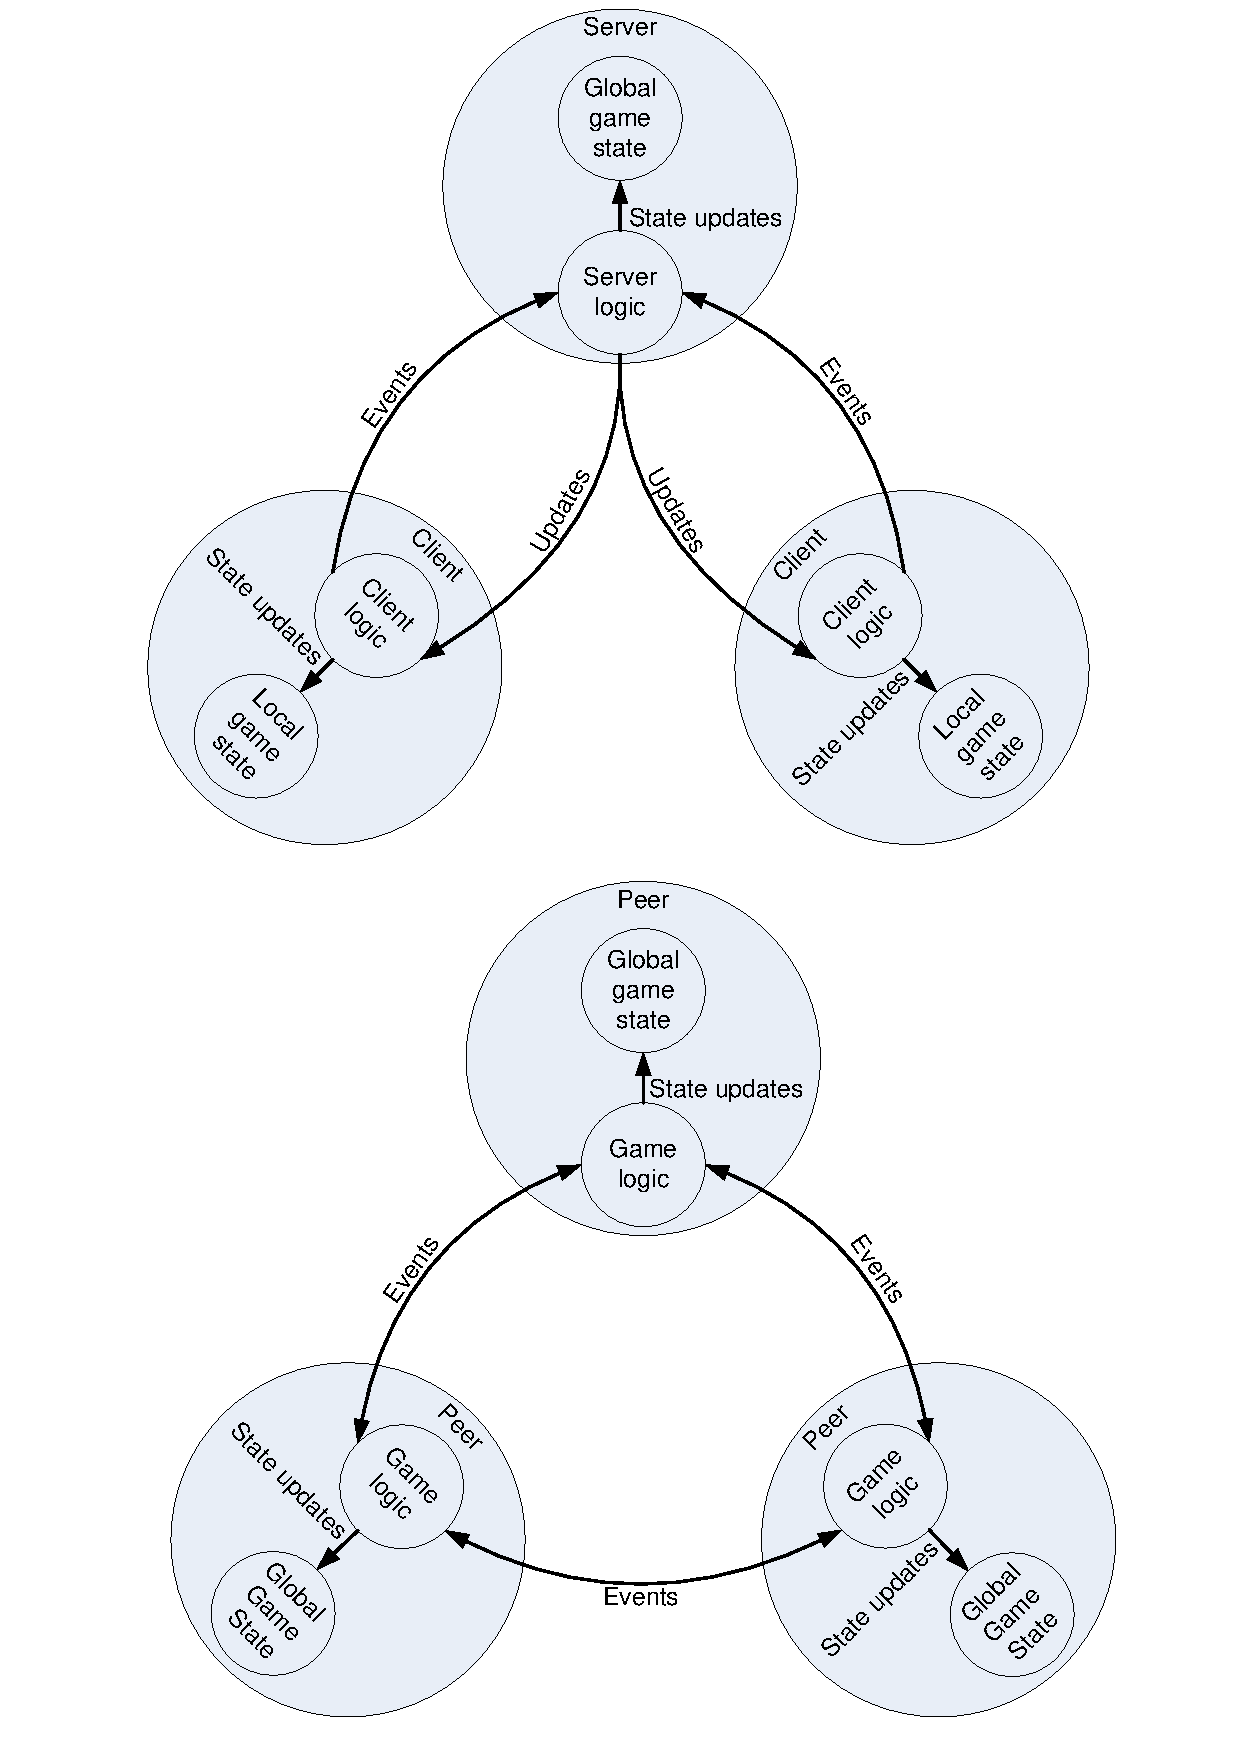
\includegraphics[clip=true, viewport= 2.5cm 0.5cm 19cm 15cm, width=0.5\columnwidth]{CS_P2P_CMs}}
 \subfloat[Update-based (client/server)]{\label{fig_cs_cm}
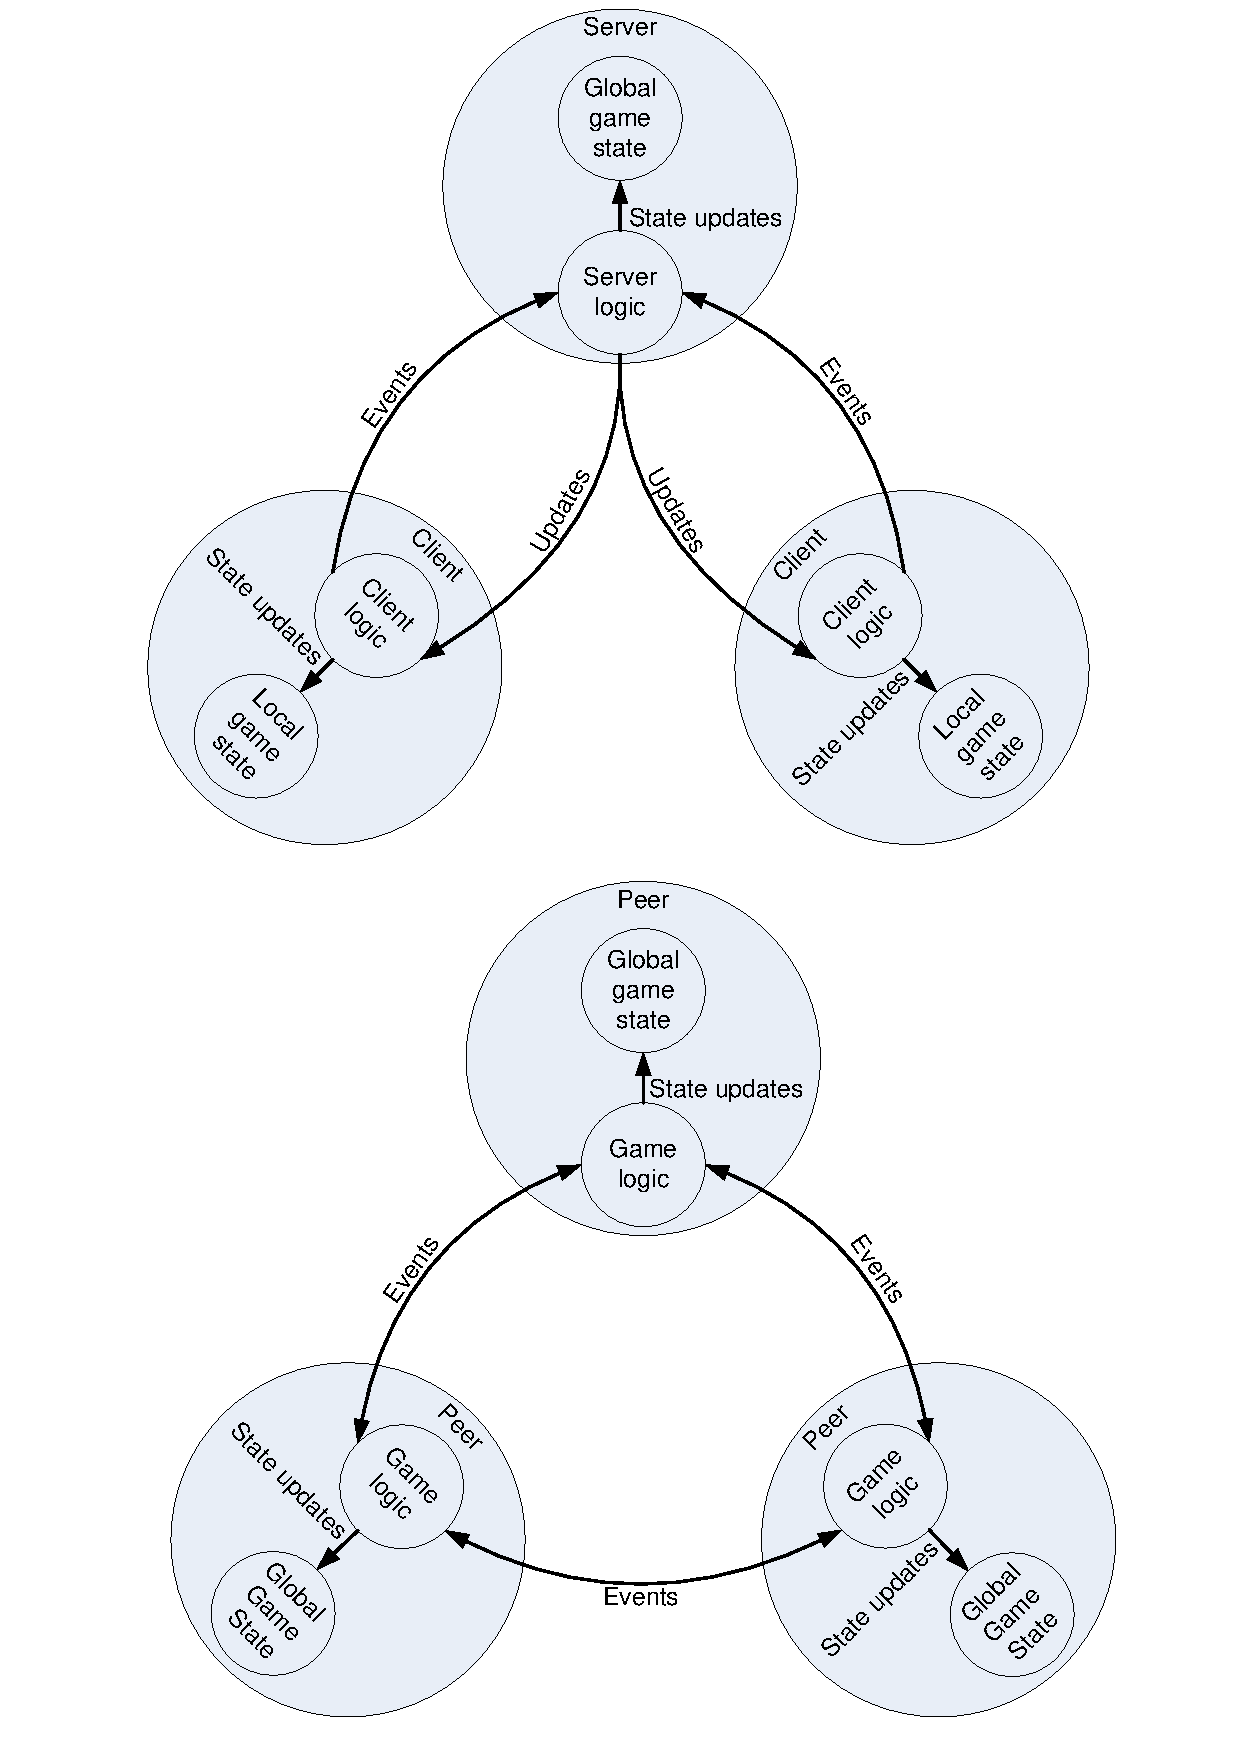
\includegraphics[clip=true, viewport= 2.5cm 15cm 19cm 30cm, width=0.5\columnwidth]{CS_P2P_CMs}}
\caption{Consistency models}
\end{figure}
%
Figure \ref{fig_p2p_cm} shows the fully distributed model. Any event that a peer generates is sent to all other peers. Each peer processes all events separately and updates its own game state accordingly. This consistency model is one where there exists multiple authoritative game states.

\subsubsection{Event generation and dissemination}

With reference to the generic flow diagram in Figure \ref{fig_event_update_flowdiagram}, user agents access the VE using peers in the fully connected network. Event generation occurs on peers.

Event layer interest management is trivial, since all peers receive all updates. Every peer, therefore, requires an up-to-date list of all other peers in the network. Event dissemination typically makes use of unicast to send all events to all peers.

\subsubsection{Event ordering}
The order in which events are received should be the same for all peers, otherwise the game states of different peers may become inconsistent.
Usually some kind of lockstep technique is used to solve this issue \cite{pessimistic_lock_step}. The issue with lockstep is that it reduces the latency to twice that of the peer with the highest latency.

Various techniques have been proposed that improves the latency by introducing some deadline before which all events should be submitted. An example of this is the New Event Ordering (NEO) technique \cite{cheat_proof_event_ordering}. This, however, makes it impossible for a player with high latency to play the game with anyone other than from her own continent.

An alternative to NEO is a P2P and C/S hybrid scheme, called the referee anti cheat scheme (RACS) \cite{cheating_taxonomy}. The scheme proposes referees, that are similar to the C/S network model, which allow for greater resistance to more types of cheats.

\subsubsection{Game logic}
Complete game logic is housed on every peer, since every peer must be able to translate any event into a state update. The game logic will determine a set of objects that will be affected by the received event and update the affected objects accordingly.

\subsubsection{Update generation and dissemination}

The game logic housed on every peer generates state updates. These state updates are only used to update the local copies of affected objects. Each peer is responsible for keeping its environment state up-to-date.

Update layer interest management and update dissemination is not required, since all affected peers will have received the event.

\subsubsection{Root object store}

The complete game state is stored on each peer.

\subsubsection{Advantages}
The event-based model works well for strategy games, and was implemented
in Age of Empires \cite{p2p_cm_aoe} and Starcraft \cite{starcraft_network_model}.

When latency issues are not present and all players possess reasonable
latencies, the event-based model can provide for an high-degree of responsiveness, because of no extra latency being added by a server and no extra server hop required for communications.

\subsubsection{Disadvantages}
The issue with the event-based model is that it is not scalable, since all peers should connect to all other peers and every event is transmitted to
everyone. This means that as $N$, the number of peers in the network increases, the traffic increases with a factor of $N^2$. The security issues of
the P2P network model, on which this consistency model is based, are also present. Slowdown is also experienced by all players if one player's
latency is below par, since the lockstep mechanism has to wait for all events to be received for that round to conclude.

\subsection{Update-based (C/S)}
\label{classic_update_based}

An alternative to the event-based model is the update-based model, shown in Figure \ref{fig_cs_cm}. This model is based on the C/S network model.

\subsubsection{Event generation and dissemination}
Actors control clients that are able to generate events. Event layer interest management is trivial, since all events are sent to the server, usually making use of a unicast event dissemination technique.

\subsubsection{Event ordering}
\label{cs_event_ordering}

Event ordering also has to be performed on the server-side, although not as critical as for the fully distributed model. If events are processed in different orders by different clients in the fully distributed model, the game states of the clients will start to diverge and no mechanism exists to merge the diverging states.

If event ordering is not performed in the update-based model, the server might execute some events out of the order in which they were generated. The game state will, however, remain consistent, since the server informs all clients of the game state as it calculates it.

\subsubsection{Game logic}
Most of the game logic is housed on the server. This allows for simplicity of design and increases system security, since the server can verify any actions performed by a client.

Some game logic might still be housed on the clients. This will typically be the handling of low risk events that don't require a high level on consistency, for example, movement updates.

\subsubsection{Update generation and dissemination}

The game logic generates states updates, which is used to update the server's authoritative game state and is also used to inform peers able to perceive the updated objects of the object's new state.

Update level interest management is required to determine which clients can perceive the updated objects. Unicast is then used as update dissemination technique to inform the affected clients of the updated object states.

\subsubsection{Root object store}
An authoritative global game state is housed on the server and a  non-authoritative local game state is housed on all clients for display purposes.

\subsubsection{Advantages}
The update-based model is used in many, if not all, MMVEs currently in operation. This includes games like World of Warcraft, Eve Online and Ultima Online, to name just a few.

This approach greatly assists with security, as clients cannot influence the state of any other clients and every client's state depends on updates
received from the server. The server state is also termed authoritative, because if there is a conflict, the server state is always the state to
which the system is expected to return. All the security advantages of the C/S model also apply to this consistency model.

Another reason why the update based model is successful is because it is more scalable then the fully distributed model. More hardware can be used to build a more powerful server, which can handle more clients.

\subsubsection{Disadvantages}

The main disadvantage is the high cost involved in obtaining and maintaining the computer clusters and server hardware, required to host the VE.

\section{P2P MMVE state consistency models}
\label{p2p_mmve_state_consistency}

An issue with the development of P2P MMVEs is that no complete consistency model has been proposed and implemented. Various schemes have been proposed to address the various challenges of P2P MMVE state consistency, but these have mostly occurred in isolation. Some of the proposed schemes will be reviewed. What should be noted is that the various areas of state consistency is quite modular, which might allow for the integration of the best schemes in each area into a comprehensive P2P MMVE state consistency model.

P2P MMVE schemes are based on one of the two classic consistency models described in Section \ref{classic_models}. Although it might seem that the fully distributed model is a better fit for P2P MMVE state consistency, this model has received less attention than the C/S model. The reason for this is partly because of the difficulties in getting the fully distributed model to scale. Usually the fully distributed model makes use of rounds, where players submit actions and all player actions are executed at the end of a round. In an MMVE with tens of thousands to millions of players, designing the round mechanism to remain scalable is a challenge. Rounds are required, because of the event ordering mechanism that ensures state consistency.

The C/S consistency architecture is applied to P2P MMVEs by distributing authoritative objects. Every authoritative object is maintained by a single node, that received all events for the object, applies the game logic and informs all nodes of the generated game updates. This effectively creates a C/S consistency model from the perspective of each authoritative object. An example of such a consistency model is the region-based model.

A region is usually created by segmenting the world and super peers act as regional servers to all peers in their region. Each super peer receives all events, handles all game logic and distributes updates to all peers in its region. The super peer also handles state management and persistency for its region, hosting NPCs, objects and persistent player data. Clients in the region only house copies of the regional objects and some client logic to update the local copies of objects.

\begin{figure}[htbp]
 \centering
 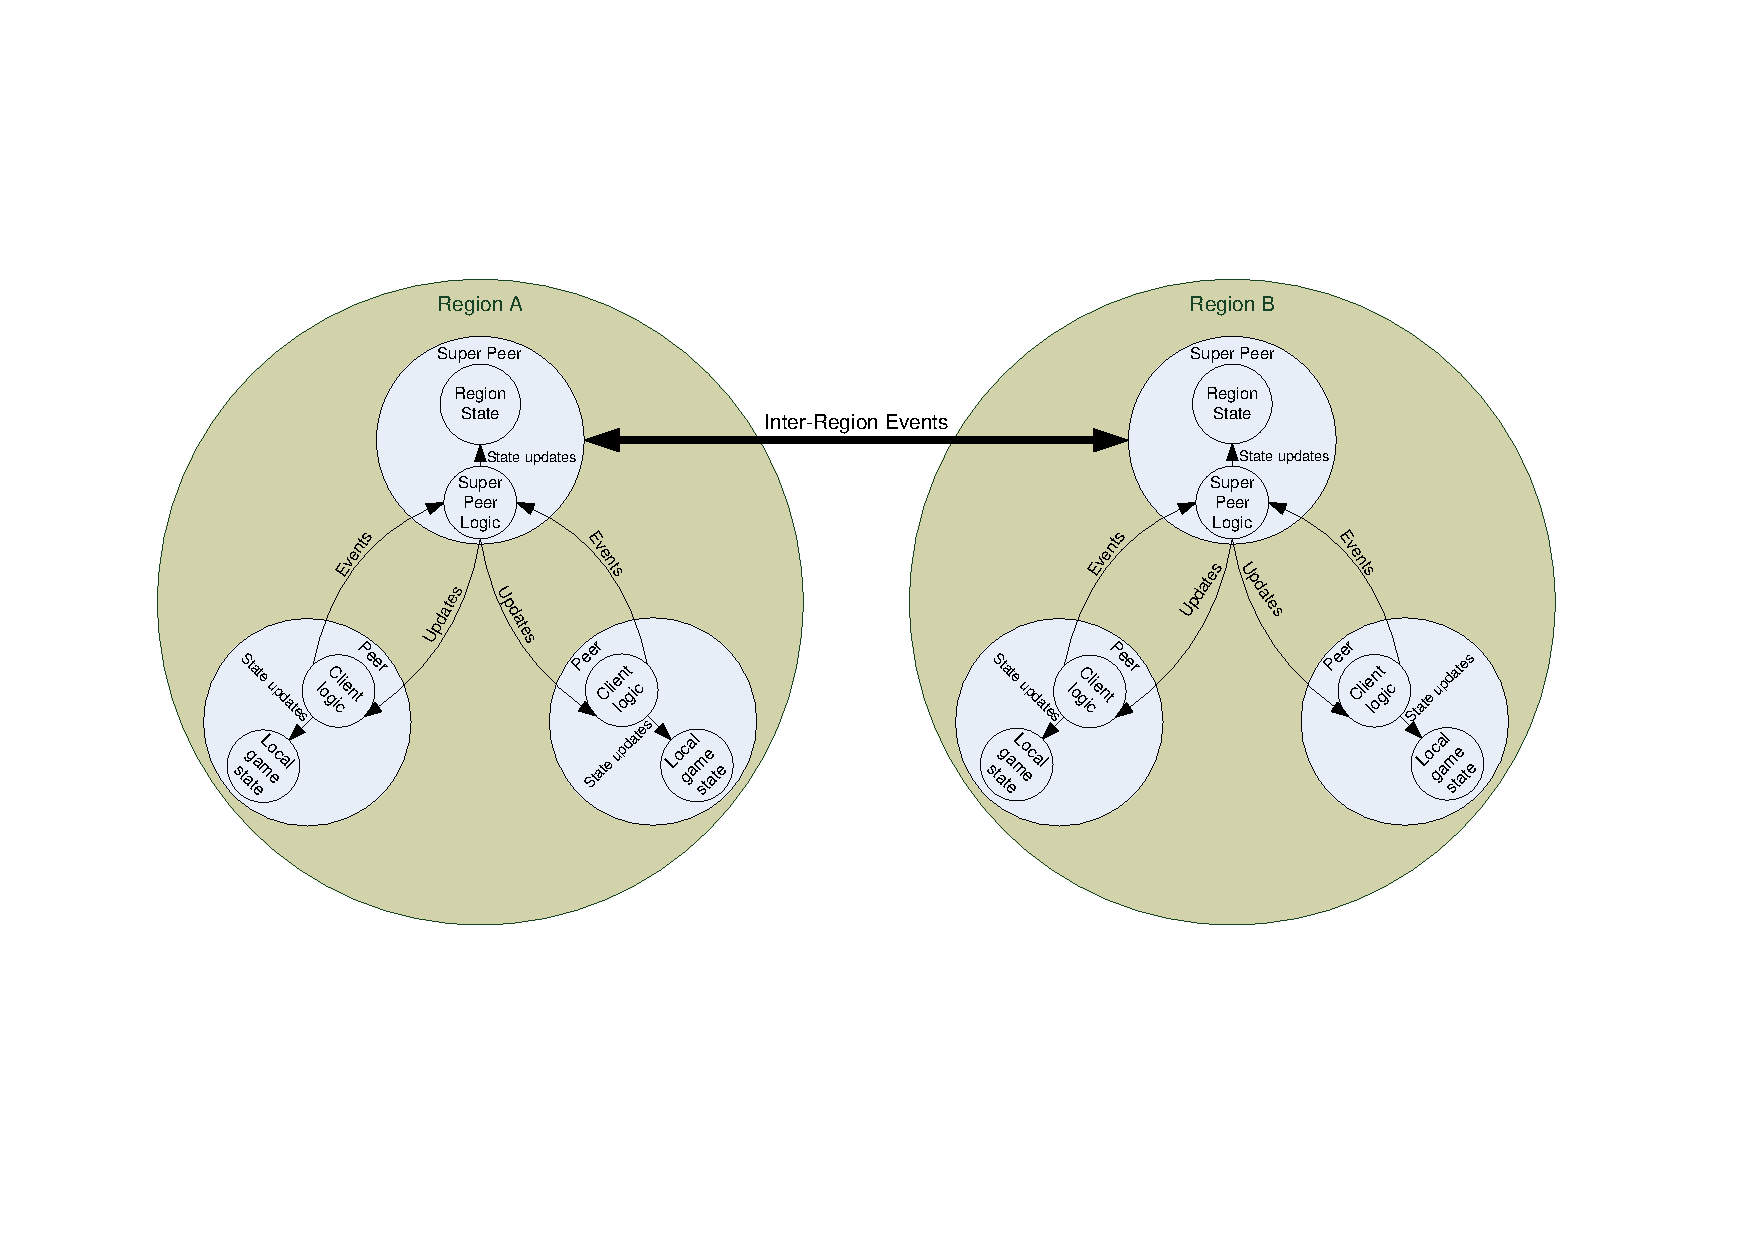
\includegraphics[clip=true, viewport=2cm 5cm 27cm 16.5cm, width=\textwidth]{region_based_CS_CM}
 \caption{Region-based Client/Server consistency model}
 \label{fig_cs_region_cm}
\end{figure}
%
The consistency model is depicted in Figure \ref{fig_cs_region_cm}. One can see that this approach is modelled on the update based model, but segmented into separate regions. The role of the server is here fulfilled by a super peer, which is a peer that is selected in some logical way, from the available set of peers and then promoted. Server selection in itself is a complex topic that has to deal with determining whether a peer has sufficient resources available and also whether the peer is trustworthy.

Presented here is an overview of the different techniques and general trends present in the various areas of P2P MMVEs. The overview does not presume to present an exhaustive list of papers in these
areas, rather to place the topic of state management and state persistency in context.

%Include the actual consistency models here. Region-based update-based, fully distributed

\subsection{Event generation and dissemination}

In P2P networks, each peer contains an agent that represents a player. Each peer can, therefore, generate events that have to be transmitted to the peers containing the authoritative objects affected by the generated event.

Recently, ALM and unicast techniques of event dissemination have become popular, depending on the grain of the event dissemination. ALM is used, instead of router level multicast, because of a lack of general support for this technology at the router level \cite{ip_multicast_deployment_issues}.

ALM is used for coarsely grained interest management techniques, while unicast is used for finely grained techniques. Unicast is not used for
coarsely grained techniques, because it is not scalable. For a network with $N$ nodes, $N^2$ messages are exchanges for every player action. ALM,
however, significantly increases the message latency in the system, because messages first have to be routed over a structured overlay network. ALM
is however preferred over unicast for large numbers of messages, because of the weak scalability of unicast.

An ALM scheme has recently been proposed, that sends updates to locations in the virtual world, rather than specific players
\cite{Ghaffari_Delaunay_churn_mobility}. This removes the need to first determine which nodes will be affected by an event, before the event may be
transmitted. Another ALM scheme proposed sends messages to the AoI neighbours, instead of to all the players in the region
\cite{Seeger_area_based_gossip_multicast}. This effectively implements a basic interest management scheme, where only neighbouring players can
receive events.

\subsection{Event ordering}

The presence and complexity of event ordering depends on the consistency architecture on which the P2P MMVE is based. In systems that use the update-based (C/S) model, no papers have addressed the issue of event ordering, since events delivered out of order will not lead to an inconsistent state, as discussed in Section \ref{cs_event_ordering}.

Where distributed architectures are proposed for P2P MMVEs, event ordering is of high importance. Designers of P2P MMVEs are making use of the same event ordering mechanisms used in the fully distributed model \cite{hybrid_storage1}.

To support a large number of players using an event-based model, event ordering with the concept of interest has been developed using N-trees \cite{GauthierDickey_ntrees}.

\subsection{Game logic}

In P2P architectures, the game logic for all objects have to be housed on all nodes, since any peer can be selected to store any object. The game logic itself is, therefore, usually distributed with the game along with the terrain and makes up the static game content. This is not to say that the game logic cannot change, but that a change in game logic will be in the form of a game update, which occurs while the game is off-line.

\subsection{Update generation and disseminiation}

In P2P MMVEs, update generation is done by the peer containing the authoritative object. When the peer receives an event, game logic is applied to generate an update. This update is then disseminated to all peers that contain agents that can perceive the object state to which the update pertains. This is similar to the update-based consistency model discussed in Section \ref{classic_update_based}.

\subsection{Update and event layer interest management}
\label{key_challenges_im}

Interest management has to occur both in the update and the event layer. For the event layer, the set of nodes has to be found, which house the root object affected by the generated event. For the update layer, the set of nodes has to be found which house the agents that will perceive an object update. What is common to both layers is that a message has to be sent to a subset of nodes with interest in the message and the interest management mechanism must determine what that subset is.

Thus far in P2P MMVE literature, little attention has been paid to whether the interest management in question is developed for the event layer or the update layer. Most discussions assume a layer and all the descriptions of the algorithm are based around the terminology of that layer. That is not to say that the algorithm itself might not be traversable to the other layer, just that this was never considered. Some interest management schemes for P2P MMVEs will not be reviewed along with the layers these schemes were designed for, but because of the similarities amongst the two layers, some schemes might be applicable to both.

Interest management is used to determine the smallest amount of information that a peer requires, in order to present an accurate representation of
the world to players. In consistency terms, it provides a means to determine which replica objects require updates of the root object. The idea is
not specific to P2P MMVEs and was already formally suggested in \cite{First_IM} and later with greater focus on a distributed environment in \cite{Whang_agent_based_IM}. Extensive research has been done into solving AoI problems and a comparison of techniques can be found in
\cite{Boulanger_IM_compare} and \cite{IM_and_ED_survey_Krause}.

The main idea is that a player has a limited visual range and area around the player in which it can interact with objects. The player requires
update information of all objects in this area, called the player's Area of Interest (AoI). AoI calculations also rely on the fact the a player's
direction and velocity of movement cannot change instantaneously and are bounded in magnitude.

Extensive research has been done into solving AoI problems and a comparison of techniques can be found in \cite{Boulanger_IM_compare} and
\cite{IM_and_ED_survey_Krause}. The solutions range from aura/nimbus \cite{Benford_spatial_IM} to publish/subscribe  \cite{mercury_publish_subscribe} to Voronoi based models \cite{Hu_voronoi_IM},  \cite{Buyukkaya_voronoi_state_management} to hybrid models \cite{hybrid_IM}, \cite{MOPAR}, \cite{fan_mediator_paper}.

Generally, interest management solutions can be divided into coarsely or finely grained solutions, although the hybrid models, especially MOPAR, seem to have gained greater popularity because they seem to have all the benefits of the two solutions and little of the drawbacks \cite{MOPAR}. MOPAR has
been shown to perform better than either a finely grained technique or a coarsely grained technique.

Coarsely grained solutions usually divide the game world into multiple regions and when a player enters a region, it subscribes to that region's
events. This is called the region-based publish subscribe model \cite{Fan_deisgn_issues_p2p}. All players in the region then receive the region's events, even for players not in their AoI.

Finely grained techniques create groups of players from their AoI. Groups of interacting players directly exchange information, so all players
only receive information that is relevant to them. This has been termed the spatial model \cite{Fan_deisgn_issues_p2p}. The grain of the solution in
turn determines the type of event dissemination that should be used, as described later in this section.

Another example of finely grained interest management was presented in \cite{IM_frontier_sets}. Interest management was achieved by making use of
frontier sets and this was implemented in Quake 3. By using Frontier Sets, it is possible to describe an area in which a player may move, where no
other players will require updates of that movement. Conversely, a set of other players that require movement updates from a specific player is also
given by the frontier set.

MOPAR partitions the game world into hexagonal regions and appoints ``home'' nodes to act as bootstrap nodes for each region. A home node of a region
is that node whose ID is the closest match the the region ID. This allows any node to find the home node for a region. A master node is then selected
for every region, whose function it is to inform slave nodes of new neighbours. All slaves nodes in a region register at their region's master node.

Slave nodes send direction and velocity updates to their masters. Masters communicate directly with other masters if a node is about to enter their
region. Masters inform their slaves of a new neighbour. Slaves communicate directly with each other, once identified by a master.

\subsection{Root object store}


In a recently completed PhD on the subject of P2P MMVEs, Lu Fan had this to say about state persistency: ``Game state persistency is a major challenge for P2P MMVEs as existing P2P storage infrastructures are designed to support file sharing, and seldom fulfil the performance and security requirements of a MMVE. \ldots the persistency area is still immature with many problems waiting to be investigated.'' \cite{Fan_phd}.

State persistency is treated as a sub domain of state consistency, in that state persistency models define where and how the root or authoritive
objects are stored. It is assumed that replica objects are always stored in the primary memory of the clients that immediately require the
information contained in the root object.

The issue of game state persistency in P2P MMVEs is the focus of this paper and the remainder of the paper will deal exclusively with this subject.
However, before the different storage types are reviewed, some classic C/S models are presented for comparison with the fully distributed model.

\section{Conclusion}

This chapter introduced the event-update consistency model that is mostly used in MMVE. From the literature reviewed, a generic process was developed that will ensure state consistency. Classic state consistency models were introduced and it was shown how these models relate to the generic state consistency process. After this, state consistency for P2P MMVEs were described. It was shown how the models used are all based on the classic consistency models. Some research into every area of P2P MMVE state consistency was discussed to enable the reader to place the work done here, into perspective.

In this chapter it was shown that the field of P2P MMVE state consistency is a growing one, already containing many significant contributions. But is was also shown that there is still much room for improvement on how we think about state management and state persistency and that there are still many open questions in these fields.

\chapter{P2P MMVE state management and persistency}
\label{p2p_MMVE_state_persistency}
%%%%%%%%%%%%%%%%%%%%%%%%%%%%%%%%%%%%%%%%%%%%%%%%%%%%%%%%%%%%%%%%%%%%%%%

\section{Introduction}

While the previous chapter broadly introduced all the concepts of state consistency, this chapter will focus solely on state management and state persistency in P2P MMVEs. The implementation of state management and persistency in P2P MMVEs allows for the storage of game data. The fact that game data must now be distributed amongst various peers in the network creates challenges not usually present in classic C/S MMVEs.

This chapter classifies the techniques used in documented P2P MMVE architectures and discusses the advantages and disadvantages of the different types of storage. The chapter also shows that no current storage type is well suited to P2P MMVEs. As the field of P2P MMVEs is a growing one, it is believed that a comprehensive survey of storage techniques is required to act as a basis for further research into the field. To the best of our knowledge, such a classification, where a focus is placed specifically on state management and persistency in P2P MMVEs, has not been undertaken in the literature.

This chapter identifies storage techniques used in P2P MMVEs. To achieve state management and persistency in P2P MMVEs, a type of distributed storage is required. Two classic distributed storage architectures are the Network File System (NFS) \cite{NFS4_protocol} and Coda  \cite{Kistler_Coda_disconnected}. There are, however, some major differences between the requirements of a P2P storage model and the classic distributed file storage model.

Firstly, NFS and Coda still require servers. One of the main advantages of P2P MMVEs is that servers are, for the most part, not required. The other requirement is low latency file storage and retrieval, discussed in Section \ref{char_responsiveness}, which NFS and Coda also do not address. Conflicts are also an issue with the Coda system, which allows multiple nodes to modify the same object. Despite the many differences, the divergent applications share some of the same requirements, namely: scalability, reliability, security and responsiveness.

The requirement of disconnected operation is generally not applicable to most interactive online games, where a player has to stay connected to the world, to be able to interact with it. One area where disconnected operation is of interest to game state management and persistency is in the area of mobile gaming. A major challenge for mobile games is the large variances in network latency. Such networks require games that are resistent to network jitter.

One approach has been proposed in \cite{Chandler_disconnected_games}, where every game client serialises its game state and distributes this game state to all other clients. Each client then creates some target game state from all received game states as well as its own state. The game client then attempts to manipulate all NPCs in the game in order to achieve the target game state. The target game state is constantly updated and thus remains a moving target. This is a new type of consistency model with many research opportunities.

\section{State management and state persistency}
A discussion of state storage requires an understanding of the difference between state management and state persistency. These terms are regularly confused in the literature and sometimes one is used where the other is more appropriate. Other times, authors describe both mechanisms as if it is all part of the same model.

In this work, state persistency is defined to mean long term data storage. Meaning that if a server or client goes off-line, the state persistency mechanism will ensure the safe storage of the state for when the server or client starts up again. State persistency is, therefore, storage in secondary persistent memory. All servers require state persistency to back-up the VE state in case of some outage or in case a server restart is required. This storage type does not have to be fast, but it has to be reliable. State persistency in P2P MMVEs is therefore taken to mean the same. It does not have to be fast, but when a client logs out of the VE and logs back in again, the stored state should remain.

State management on the other hand is defined to mean the storage of the VE state in primary memory. This is the state with which the server and clients will interact. It is the state that will be displayed to the agent on the client and it is the state that will require fast reads and writes as consequences of received events or updates. Every time an object update is generated, it will be applied to the objects by state management. Every time the game logic requires the information of other objects to determine which update to generate on account of a received event, it will make use of state management.

Although these are two different types of storage, with different storage requirements, there are also aspects of state management and persistency that are the same. The similarities and differences will be reviewed in Section \ref{key_challenges_cm}. The similarities between state management and state persistency are explained in this chapter by using the generic term ``storage''. There are many ``storage types'' that will be introduced in this chapter. These storage types can either be state management or state persistency. The relevance of difference storage types to state management and consistency will, however, be discussed.

\section{Client/Multi-Server state management and persistency models}
\label{cms_models}

This section introduces the classic state management and persistency architectures used in server cluster or client/muli-server based systems \cite{Hu_voronoi_IM}.

\subsection{Sharding}

A storage model where the VE state is duplicated over multiple servers, with players connecting to one of these servers is termed ``sharding''. Clients are not able to interact or communicate with players on other shards, which reduces game immersion. This method does, however, allow for a more scalable system as maximum load is fixed.

Players are not able to enter a shard if that shard has reached its capacity. In the past, this has caused unhappiness amongst players, since popular
shards could be difficult to log in to. Players are also reluctant to move to a new shard, because a lot of time is invested in their characters in
their ``home'' shard. Sharding doesn't allocate resources efficiently, as one shard may be overpopulated while another is underpopulated. For all
practical purposes, this approach is still merely a C/S approach, with players forced into a specific C/S environment.

The benefit of sharding is its ease of implementation and the reduction of content designer load. Because no inter-server communication is required
and no server migration is supported, this method greatly simplifies the server design process. Another benefit of sharding is that it allows for a
relatively small game world to support many players because of the duplication of the worlds. This reduces the load on level designers and content
designers, who now have to populate a much smaller world with content.

\subsection{Replication-based}
%Redundant
The replication-based model is similar to sharding, with the difference that all servers share the same duplicated game state. Each server contains
the global game state and clients connect to any one of these servers (mirror-servers \cite{mirrored_server}) or through a load distribution
algorithm to a server (proxy-servers \cite{proxy_server_dist}). Each server handles all actions from clients and updates its own database. The
servers in turn send updates to each other over a high quality link, such as fibre, to maintain database consistency at high speeds.

The problem with this system is that the world is never truly consistent and that there are no optimally chosen inconsistency obfuscation boundaries.
In other words, two players standing next to each other in the virtual world, might be on different servers and, therefore, experience two slightly
different worlds.

\subsection{Object-based}
%Object based
The object-based storage model equally distributes all in-game objects amongst the servers \cite{object_based_consistency1}, \cite{object_based_consistency2}, \cite{object_based_consistency3}. For an MMVE, most of these objects are expected to be player objects. The advantage of this method is that the system load is fixed for a certain player population and that the load is equally distributed amongst all servers. This allows for more accurate prediction and provisioning of resources, but still does not handle transient loads
well.

Another issue is inter-server communications for this architecture. The inter-server communications are random and also more than the inter-server
communications for a region based system. The reason for this is that the number of player interactions increase with a decrease in the distance
between the players. Players playing together move together, chat and interact with NPCs together. For a region based model, all player-neighbour
interactions remain local to the server.

\subsection{Zone/Region-based}
%Zone-based
The zone-based storage model divides the virtual world into zones or regions, which are hosted on different
servers \cite{zone_based_stat}, \cite{zone_based_dyn}. A well known example of this model is Eve Online. Busy regions are hosted on their own
servers, while multiple quiet regions are hosted on a single server. This is termed the static region approach \cite{zone_based_stat}.

The issue of the static region approach is that it does not scale well when one region is suddenly populated with players. This type of behaviour
happens quite regularly and is known as flocking \cite{flocking}. When players find something of interest in a region, many players will flock to
that region. The solution to flocking has been over provisioning of resources to handle peak loads, which suffers from the disadvantages discussed above. Also, if the load changes, the server has to be brought off-line in order to balance the regions.

Dynamic regions are being investigated, where regions can be dynamically shifted from one server to another, in order to balance load
\cite{zone_based_dyn}. This approach adds overhead and significant complexity with regards to the migration of the data and the handling of player actions while the data are in transit.

\section{P2P MMVE storage requirements}
\label{key_challenges_cm}

%Consistency issues
The key challenges related to P2P MMVE storage models are: scalability, reliability, responsiveness, security and fairness. All storage models will be reviewed with these characteristics in mind. In order to evaluate any storage model, metrics have to be defined to measure the key characteristics of a storage system. This will allow for different storage models to be compared and provide a measure of the applicability of any storage model to P2P MMVEs.

\subsection{Scalability}
\label{scalability_req}
Scalability underpins all evaluation criteria. This implies that for a system to be scalable, all other evaluation criteria should be satisfied for
large numbers of nodes and data. For this reason, scalability will not be explicitly reviewed in the following storage types. Rather, all other
evaluation criteria will be evaluated for a large number of nodes, thereby taking into account scalability.

The question of what constitutes a large number of nodes arises. To establish what an adequate number of nodes is, current MMVE architectures can be
used for inspiration. It is proposed that to classify a system as \emph{sufficiently scalable}, the smallest number of peers that should be used is
approximately 3000. This is the number of players per server, currently supported by most active C/S MMVEs. For a system to be classified as
\emph{truly scalable}, it is believed that the architecture should support 60,000 concurrent users, twenty times more than a sufficiently scalable
system. This is the number of peak concurrent users (PCUs) currently supported by the super computer used to host Eve Online \cite{eve_pcu}. These
two measures will ensure that a system is as scalable as other currently available architectures.

For systems that will support the MMVEs of the future, it is believed that a target of 1 million nodes should be used. This number is sixteen times
that of a truly scalable system and the peak concurrent player count of World of Warcraft in China in 2008 \cite{WoW_china_pcu}. Systems that will
support these numbers can be classified as \emph{highly scalable}. It is important to note that no current systems support such a large PCU count on
a single server cluster. The PCU count presented for WoW is the PCU count over all server clusters hosting WoW in China.

\subsection{Fairness}
Ensuring fairness in the system means distributing load evenly according to the abilities of individual nodes. This ensures that not only a small
number of nodes provide all system resources required for the system to function, but that all nodes contribute what they can, in order to support
the system.

Fairness does not exclude heterogeneity of nodes. It is accepted that nodes have different amounts of available resources. It also does not exclude node specialisation. It is accepted that some P2P architecture require specialised nodes or require a set of different types of super peers to function. Fairness merely states that when all node contributions have been counted, the sum of node contributions should be equal.

Fairness can be evaluated by evaluating the distribution of game state amongst all nodes in the P2P network. This can be measured at a file level,
i.e. what is the standard deviation of the number of files contained on each node, or on byte level, i.e. what is the standard deviation of the number of bytes stored on
each node. A lower standard deviation will point to a fairer data storage scheme, if it is assumed that all nodes should contribute an equal amount of storage.

\subsection{Reliability}

For the storage to be reliable, it must be impossible for data to be lost, and stored data should always be available when a node requests it.
Reliability encompasses both robustness and availability. Robustness means that the data should be resilient to network churn and availability means
that data should be available to any node in the network, with the correct permissions.

Reliability can be measured as the percentage of successful storage and retrieval requests, compared to the total number of storage and retrieval requests.

\subsection{Responsiveness}
\label{char_responsiveness}

Responsiveness is the only requirement that is less important for state persistency, compared to state management. Because state persistency merely acts to back-up the data, fast storage or retrieval is not as important as it is for state management. Highly responsive state persistency will still improve data throughput and ensure that less data will be lost in the event of a failure, but highly responsive state management is required for the correct functioning of the state consistency mechanism.

To ensure system responsiveness, objects must be stored or retrieved in real-time. With real-time, it is meant that data should be available within a
certain time frame that would ensure correct functionality of the MMVE requiring it. The variance in data retrieval times should be small. Responsiveness can be measured by the time it takes to read or write data to the storage network.

\subsection{Security}
\label{characteristics_security}

The storage system should store data securely. It should not be possible for data to be altered in ways that are inconsistent with the game rules. It
should also be possible to identify nodes that alter the data in a malicious way. This also adds the requirement that nodes should be authenticated
in the storage system and that only authorised nodes should be able to alter data. Security is the combination of a number of objectives:
Authentication, Authorisation, Data Integrity, Confidentiality, Availability, Trust, Privacy and Identity Management
\cite{distributed_systems_security}.

For a storage model to address the security objectives of authentication, authorisation, confidentiality, trust, privacy and identity
management, a certification scheme with public and private key encryption is required. Such a scheme allows for the identification of users, and by
having users sign any storage interactions, every change made to the storage system can be tracked. This is a major differentiating factor from
classic distributed storage systems such as Freenet, where a primary objective is anonymity. If all operations are logged and all users have to be
identifiable for a secure system, no users can be anonymous.

\section{Overview of P2P MMVE storage types}
\label{storage_type_overview}

%Overview of four approaches
Four approaches have been identified by which state persistency is achieved in P2P MMVEs: \emph{super peer storage}, \emph{overlay storage}, \emph{distance-based storage} and \emph{hybrid storage}. These four storage architectures are detailed in Sections \ref{super_peer_storage}, \ref{overlay_storage}, \ref{hybrid_storage} and \ref{distance_based_storage}.

%Centralised storage
Two other types of storage sometimes described in P2P MMVEs papers are \emph{centralised storage} and \emph{individual storage}. Centralised storage is storage in a centralised database, the same as for a C/S MMVE \cite{badumna_engine}, \cite{rooney_centralised_storage}, \cite{hybrid_p2p_cs_centralised}. Centralised storage for an MMVE requires the same large expensive servers and high bandwidth as required by a classic C/S architecture and therefore does not fit into the P2P MMVE paradigm. For this reason, centralised storage will not be evaluated in this chapter.

%Individual storage
With individual storage, player data are stored on a player's own computer \cite{individual_storage1}, \cite{cheat_proof_playout}. These
architectures do not address the storage of NPC state or mutable objects. These objects cannot be as easily mapped to a single node in the network as
player state can and, therefore, require a mapping mechanism to decide where to host these objects. Individual storage will not be explicitly discussed
in this chapter, however, individual storage can be regarded as a subset of distance-based storage, which will be discussed in detail in Section
\ref{distance_based_storage}.

\begin{table}[htbp]
\centering
\begin{tabular}{|r|c|c|c|c|c|l|}
\hline
Storage type & Reliability & Responsiveness & Security & Fairness & Complexity & Examples\\
\hline
Super Peer & Medium & High & Low & Low & Very Simple & \cite{knutsson_p2p_first}\\
Overlay & High & Low & Medium & High & Simple & \cite{Douglas05enablingmassively}, \cite{using_freenet_storage},
\cite{Fan_phd}, \cite{past_storage_focus}\\
Hybrid & High & High & Medium & Low & Complex & \cite{zoned_federation}, \cite{hybrid_storage1}\\
Distance-based & Medium & High & Low & Medium & Very Complex & \cite{Buyukkaya_voronoi_state_management}, \cite{Hu_voronoi_IM},
\cite{colyseus_distance_based}, \cite{solipsis}\\
\hline
\end{tabular}
\caption{Differences between storage mechanisms} \label{tab_storage}
\end{table}
%
Table \ref{tab_storage} presents a characterisation of current storage systems according to the characteristics defined in Section
\ref{key_challenges_cm}. Table \ref{tab_storage} also provides some references that act as examples of the different storage types mentioned. These
example architectures will be discussed in detail in the sections to follow. The purpose of the complexity category in Table \ref{tab_storage} is to
provide a measure of how difficult it will be for an application developer to use any of the storage types and is discussed in Section
\ref{recommendations}.

\section{Super peer storage}
\label{super_peer_storage}

%Super peer storage - description
Super peer storage makes use of the region-based P2P MMVE consistency model described in Section \ref{p2p_mmve_state_consistency}. Super peer storage relies on the super peer storing all information that is in its region.

\subsection{Fairness}
%Super peer storage - issues
The super peer storage model has many potential issues. Overloading of the super peer is one. A super peer could be relatively easily overloaded if a
region becomes too crowded, since a super peer is merely the computer of some player in the game and not a specialised server machine. The question
of fairness also arises. The idea of a P2P MMVE model is that all peers share resources. With this model, peers with extra resources are expected to
donate these resources for the good of all. Players might consider it unfair, when they are constantly expected to donate resources, some of which
they might have to pay for, while other players never contribute.

In a system with lower fairness, the individual user load is also higher for those users that do have to contribute resources. This means that in an
unfair system, the users that do have to contribute, have to contribute more than what they would have, were it a fair system.

\subsection{Reliability}
\label{super_peer_storage_reliability}

In a P2P system, with a high rate of churn, players are expected to constantly leave and join the network. Because of this reality, redundancy
mechanisms have to be developed that would ensure state data are always available, even when a super peer leaves the network. It is possible to solve
these issues by having redundant super peers in each region that take over hosting responsibility when the main super peer leaves.

It is important that the main and backup super peers always possess consistent states, even during a transition from main to backup. Other schemes to
support improved reliability deal with reputation mechanisms for super peers. Super peers that have more resources and stay in the network longer are
preferred during super peer selection, using reputation mechanisms \cite{fan_mediator_paper}.

\subsection{Security}

Probably the most important issue is that of security. If a single peer is allowed to house the player information of a large group of players, it
might become possible for such a peer to maliciously modify the data. The issue is not only that modification of the data might be possible, but also
that it would be impossible for the cheating to be detected, because of no centralised logging. Locally obtaining access to data will circumvent the
protections created by a certification system, which would then pose a threat to all security objectives protected by the certification system as
mentioned in Section \ref{characteristics_security}.

A scheme that would improve the reliability of this systems has been proposed, where every event is also sent to the backup super peer of the region
\cite{past_storage_focus}. The main super peer responds with the update and the backup super peer responds with a hash of the update. A peer can then
check whether the hashes match to determine whether the data has been received correctly. A hash is not the state update itself, so will be smaller,
but the events that have to be sent to all super peers will increase traffic in the network and bandwidth usage by peers.

\subsection{Responsiveness}
There are also advantages to super peer storage. All data are stored on the super peer, which means that storing data is a low latency operation. The
regional state can be stored and retrieved at high speeds, making the system very responsive. Data retrieval from such a storage is as fast as data
retrieval from a server. Peers can request data from a super peer and the data can be returned to the peer in one hop after transmission of the
request. Super peers may, however, become overloaded with requests and thereby increase the latency of the system.

\subsection{Existing architectures}

Knuttson et al. \cite{knutsson_p2p_first} employ regional super peers called ``coordinators'', to host all shared object states. The coordinator is
chosen as the node whose ID is closest to that of the region ID. The region ID is a SHA-1 hash of the region's textual name \cite{SHA}. This mapping
makes it unlikely that the coordinator will be a member of the region. The advantages of such a selection scheme is that the opportunities for
cheating are reduced, because the data are hosted on a peer that has no or little interest in the data, as described in Section
\ref{distance_based_storage_security}.

Coordinator hand-offs also occur less than if the coordinator was an elected member of the region. If this is the case, a new coordinator has to be
chosen every time the current coordinator leaves the region. In this scheme, hand-offs only occur as a result of network churn, which is far lower
than the number of players moving from one region to another.

Reliability is achieved by maintaining backup coordinators as the Distributed Hash Table (DHT) neighbours of each region coordinator. One method by
which redundant region coordinators are maintained in \cite{knutsson_p2p_first}, is to create backup coordinators on peers with IDs closest to the
current coordinator. This means that if the main coordinator fails, all data will automatically be routed to the backup, because of the feature of
DHTs. This method is similar to how reliability is achieved in overlay storage as described in Section \ref{overlay_storage_reliability}.

\section{Overlay storage}
\label{overlay_storage}

Overlay storage is classified as using any type of structured P2P overlay to store data in a distributed fashion. This is a very broad definition,
which basically encompasses any P2P distributed storage currently in use. Some examples and a comparison of different distributed storage techniques
can be found in \cite{Hasan_distributed_storage_survey}. The reasoning is that any P2P distributed storage can be used to only store game files.
Therefore, distributed storage is used as a distributed database for game files. Whether this is an optimal solution will be discussed in the
remainder of the section.

\subsection{Reliability}
\label{overlay_storage_reliability}

Overlay storage can be made reliable, using redundancy. One method used to achieve high reliability in structured overlay storage is to store $k$
replicas for any file stored, in order to ensure the availability of the file. These replicas are stored at the neighbouring nodes of the node
containing the original file. Neighbours are the $k$ nodes whose IDs are closest to that of the root node. By the characteristics of DHT
distance-based routing, if the node with the original data leaves the network, packets will automatically be routed to the neighbouring node, which
stores a duplicate. This technique ensures high availability of data and the number of duplicates can be chosen according to the reliability of the
network.


\subsection{Responsiveness}
%Overlay storage - issues

The most significant issue with overlay storage is the delay incurred when storing and retrieving data. As data can be stored anywhere on the network
and the network is not fully connected, an average of $\OO{\log(N)}$ hops are required to retrieve or store a data item
\cite{storage_and_chaching_PAST}. Although this is a sufficient order complexity for a routing algorithm in a large network, it is not sufficient to
support a real-time application. For responsive MMVEs, a distributed file system is required that allows for real-time file storage and retrieval.

The mechanism by which churn is handled, described in Section \ref{overlay_storage_reliability}, also improves responsiveness.  This is achieved,
because IDs created by the random hash function ensures that a nodes's neighbours are distributed randomly throughout the P2P overlay. This random
distribution ensures that file replicas, stored at a node's neighbours, are uniformly distributed throughout the P2P overlay network.

%Data migration in Oceanstore

\subsection{Security}
The overlay storage model is more secure than the super peer storage model as data are distributed amongst all peers and redundancy and quorum
techniques can be implemented to ensure that files are retrieved with a high level of security.

To ensure a secure system, copies of files have to be saved at different locations. If a file is retrieved, all copies must be queried and received.
All received copies then have to be compared to ensure that the contents are correct. This introduces additional network overhead as well as
additional load on nodes to serve as file copies.

The network overhead can, however, be reduced by having file replica nodes only send hashes of the files, which may then be compared at the
requesting node. Hashes require less bandwidth, while still allowing a requesting node to check update validity by hashing the received update and
comparing with the received hashes.

\subsection{Fairness}

Overlay storage is fair, as all nodes share file data and requests equally. The system might be made fairer by taking into account the heterogeneity
of peers. Peers do not all possess the same resources, something which a truly fair system should take into account. The difficulty with using such a
scheme is that peers can be made to report incorrect resource information in order to reduce their resource donation requirement. This is where
incentive mechanisms have to be investigated as well as ways to ensure correct resource reporting.

\subsection{Existing architectures}

%Merabi, 2004 \cite{using_freenet_storage}
In 2004, Merabti and El Rhalibi mention the issue of ``Data Storage'' \cite{using_freenet_storage}. It is recognised that a distributed storage
scheme is required and that such a scheme ``\ldots requires careful designing\ldots''. They propose the use of a data storage architecture based on
the Freenet project \cite{clarke_freenet}. Freenet is a distributed storage facility that uses a Darknet to ensure user anonymity when distributing
files. A system such as Freenet is designed for general file sharing, which means that no focus is placed on achieving the high levels of
responsiveness required for MMVEs. While the need for state persistency is briefly mentioned in the 2004 paper by Marabti and El Rhalibi, Douglas et
al. implement a workable solution for state persistency in 2005.

%Douglas, 2005 \cite{Douglas05enablingmassively}
Douglas et al. designed a P2P MMVE architecture in 2005 \cite{Douglas05enablingmassively} and implemented state persistency using a distributed
storage implementation, which they developed in 2003 \cite{Harwood03hashingspatial}. The storage system allows for the manipulation of spatial data,
while also implementing range queries. This enables the system to store and retrieve data that exist in a certain area of the game world. In the MMVE
architecture they developed, state persistency is implemented by the ``Spatial Data Service'' (SDS), which is a distributed storage architecture that
uses the Chord P2P overlay for routing \cite{chord}.

%Hampel, 2006 \cite{past_storage_focus}
PAST has become a popular way to implement state persistency. This is the approach proposed by both Hampel et al. in 2006 \cite{past_storage_focus}
as well as Fan in 2009 \cite{Fan_phd}. In these publications, it is said that PAST is used to store the global game state, but never is detailed what
is stored and how regularly it is stored. Player information is supposed to be stored as game state, but from the papers it is unclear how position
updates are handled. It is not clear whether the last position of a player is stored at all or how regularly it is stored. It is important to know
how position updates are handled in the game, since position updates are the most common type of update \cite{knutsson_p2p_first}.

PAST has not gained much commercial adoption, because of the lack of support for keyword searches, which is a requirement of most distributed storage
networks, where users constantly search for content. Keyword searches are, however, not required by the storage mechanism of an MMVE. The IDs of the
items stored in the network will be known. A player's inventory can, for example, always be called \verb.(player_name)_inventory.. A hash of this
file name will find the correct file. This, and the use of Scribe, is why PAST has become popular with researchers of P2P MMVEs.

PAST \cite{PAST_storage} uses Pastry to implement a distributed storage system. Files that have to be stored are given IDs, by using some hash
function, for example SHA-1 \cite{SHA}. The file, along with the ID are sent as a message over the overlay. The messages is then routed to the node
whose ID is a closest match of the file ID, where the file is stored. If any nodes wish to retrieve the file again, it only requires the file hash. A
``get'' message can be sent to the overlay, where the overlay will route the message to where the file is situated and retrieve the file.

In an effort to increase responsiveness, PAST also employs caching techniques \cite{storage_and_chaching_PAST}. If a node forwards many queries for a
file, that node can elect to cache the file to improve the responsiveness of the system. This caching can only occur if the node has space available.
If a node has cached a file and another file is explicitly inserted into the node, it can elect to remove the cached file in order to free up space.
This means that the success of the caching mechanism is directly related to the level of storage utilisation. Higher utilisation will prevent files
from being cached.

The main difference between the implementation by Douglas et al. and the PAST implementations, is that the former supports range queries on spatial
data, which allows for a set of objects to be returned, queried by their virtual in-game position. With PAST, the exact ID of an object is required
before it may be retrieved. Using PAST is the simplest means by which game state persistency may be implemented, but PAST is not necessarily the
application best suited to game state persistency. There exists a need for more research into appropriate state persistency mechanisms for P2P MMVEs.

\section{Hybrid region-based storage}
\label{hybrid_storage}

%Overlay storage - description
\begin{figure}[htbp]
 \centering
 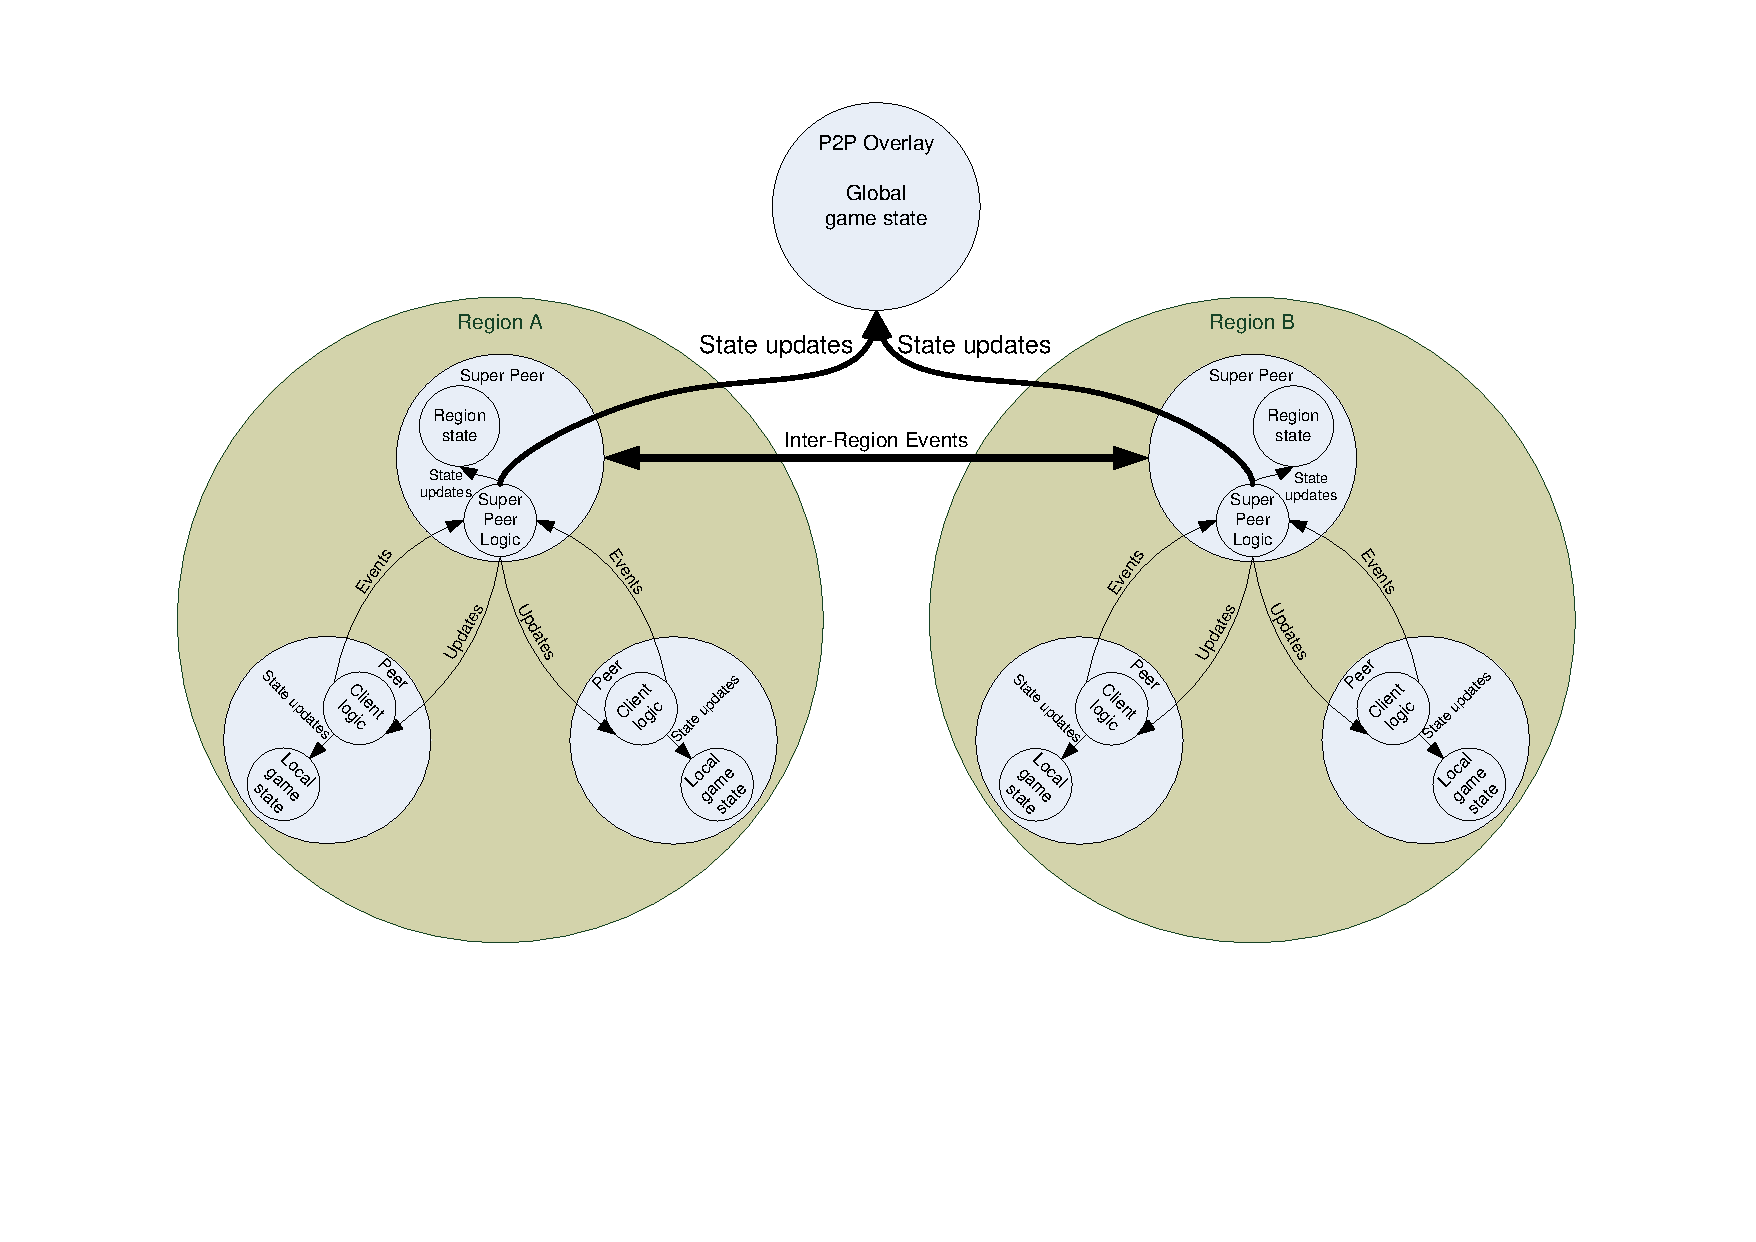
\includegraphics[clip=true, viewport=2cm 5cm 27cm 19.5cm, width=\textwidth]{region_based_CS_CM_P2PO}
 \caption{Hybrid region-based super peer storage with backup overlay storage consistency model}
 \label{fig_cs_region_o_cm}
\end{figure}
%
Figure \ref{fig_cs_region_o_cm} shows a type of Super Peer/Overlay hybrid storage implemented in \cite{zoned_federation}. The model depicted in
Figure \ref{fig_cs_region_o_cm} uses an overlay storage, managed by regional super peers. The world is divided into regions, with each region
controlled by a super peer. The complete region state is cached at every super peer, the same as with super peer storage. There also exists a backup
overlay storage architecture, to which data may be backed up for long term, redundant and secure storage. The hybrid region-based overlay storage
contains many improvements over pure overlay storage as will be discussed in the following sections.

\subsection{Reliability}
\label{hybrid_storage_reliability}

Because of the use of overlay storage for backup, the hybrid region-based storage is almost as reliable as a pure overlay storage. It is classified
as almost as reliable, because there is a delay between when data changes and when it is updated in the overlay. If a super peer fails during this
time and the data was not backed-up to the overlay, that data could be lost. Backup super peers can, however, be implemented as described in Section
\ref{super_peer_storage_reliability} to improve the reliability of the hybrid storage model.

\subsection{Responsiveness}

Because all regional files are cached at super peers, the system is as responsive as super peer storage.

\subsection{Security}

Security in hybrid storage is still an issue, because of the inherent problems of the super peer storage model. Although it is more difficult for
nodes to access and manipulate data stored in the overlay, a malicious node promoted to super peer status may manipulate the region data it controls.

It does seem possible to achieve higher levels of security, by checking data received from super peers, against the data stored in the overlay. Care
should be taken with such a scheme, because the rate of change of data at the super peers might be higher than the rate that data are submitted to
the overlay. Another issue is the time delay between data received from a super peer and data received from the overlay.

\subsection{Fairness}

The issue of unfairness is also still present in hybrid storage. The system is fairer in that all nodes share the load of the overlay storage, but
there still exists the unfairness of the super peer storage. As all data exists in both the overlay storage as well as the super peer storage, the
system is as unfair as super peer storage, because the same quantity of data as in super peer storage is not being distributed evenly amongst all
nodes.

\subsection{Existing architectures}

\begin{figure}[htbp]
 \centering
 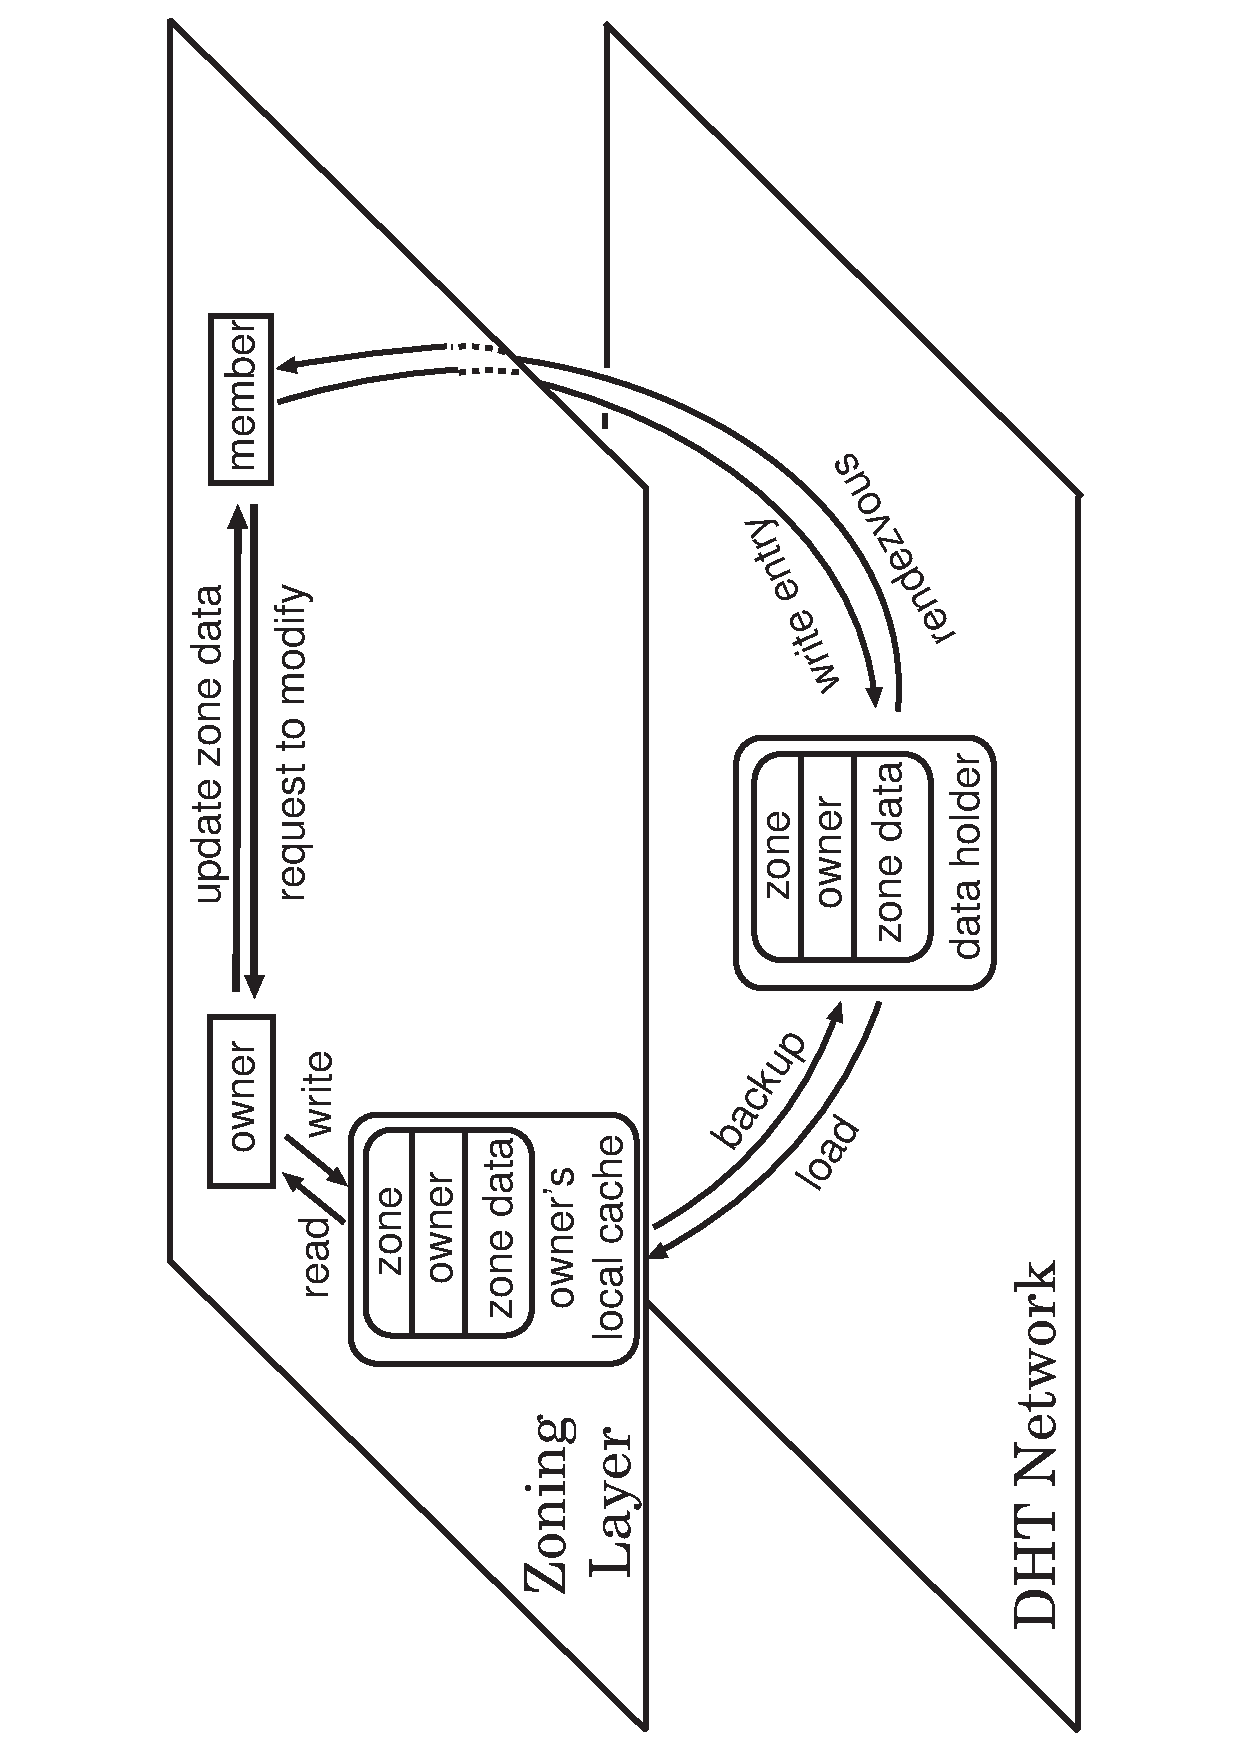
\includegraphics[clip=true, viewport=2cm 0cm 19cm 30cm, angle=-90, width=0.5\columnwidth]{zoned_federation_model}
 \caption{Zoned Federation Model \cite{zoned_federation}}
 \label{fig_zoned_federation_model}
\end{figure}
%
The first hybrid state persistency model for P2P MMVEs was proposed by Iimura et al. in 2004 \cite{zoned_federation} and called the ``Zoned
Federation Model'', shown in Figure \ref{fig_zoned_federation_model}. The regional super peers are called ``Zone Owners'', which handle all events by
clients in their zone or region. In the Zoned Federation model, a Zone Owner acts as the primary storage medium for all object states in the zone or
region. As shown in Figure \ref{fig_cs_region_o_cm}, this is analogous to an update based model, divided into zones. The difference here is that the
game state of all zone owners are regularly backed-up to overlay storage. The zoned federation model can thus be seen as a super peer/overlay storage
hybrid. The super peers storage provides for low latency data storage and the overlay storage provides security and reliability.

An extended abstract, published by GauthierDickey et al. in 2004 \cite{hybrid_storage1}, proposed to distinguish between permanent and ephemeral
data. Permanent data are described as data that should exist at all times and ephemeral data are described as data that need only exist for as long
as its owner is in the game. An item, being dropped by a dispatched NPC, can be considered as ephemeral. When the peer on which the data is hosted
leaves the area, that item can disappear. An example of permanent data is a player's inventory contents, which can further be classified as
participatory data or a player's house, which can be classified as existential data. Participatory data are data that need only be available when a
specific player is in the game and existential data are data that should be available, even when a certain player is not present in the game.

Categorising data by how long and under which circumstances the data should exist, may assist in the design of the storage model. Since ephemeral
data does not have to exist after the player has left the game, it may be stored in primary memory. Participatory data might also be stored on the
player's computer, but security issues will have to be kept in mind. Existential data will have to be stored somewhere other than on the player's
computer, since other players will require the data, even in the absence of the player that might have left the game. GauthierDickey et al. did not
explore how their data classification scheme might be translated into a state persistency model.

\section{Distance-based storage}
\label{distance_based_storage}

%Distance-based - overview
Distance based approaches, such as the Voronoi storage approaches \cite{Buyukkaya_voronoi_state_management}, \cite{Hu_voronoi_IM} and some more
general approaches \cite{colyseus_distance_based}, \cite{solipsis}, store object data on the peer closest to the object in the virtual world. Some
distance metric is used to determine on which node an object should be stored.

\begin{figure}[htbp]
 \centering
 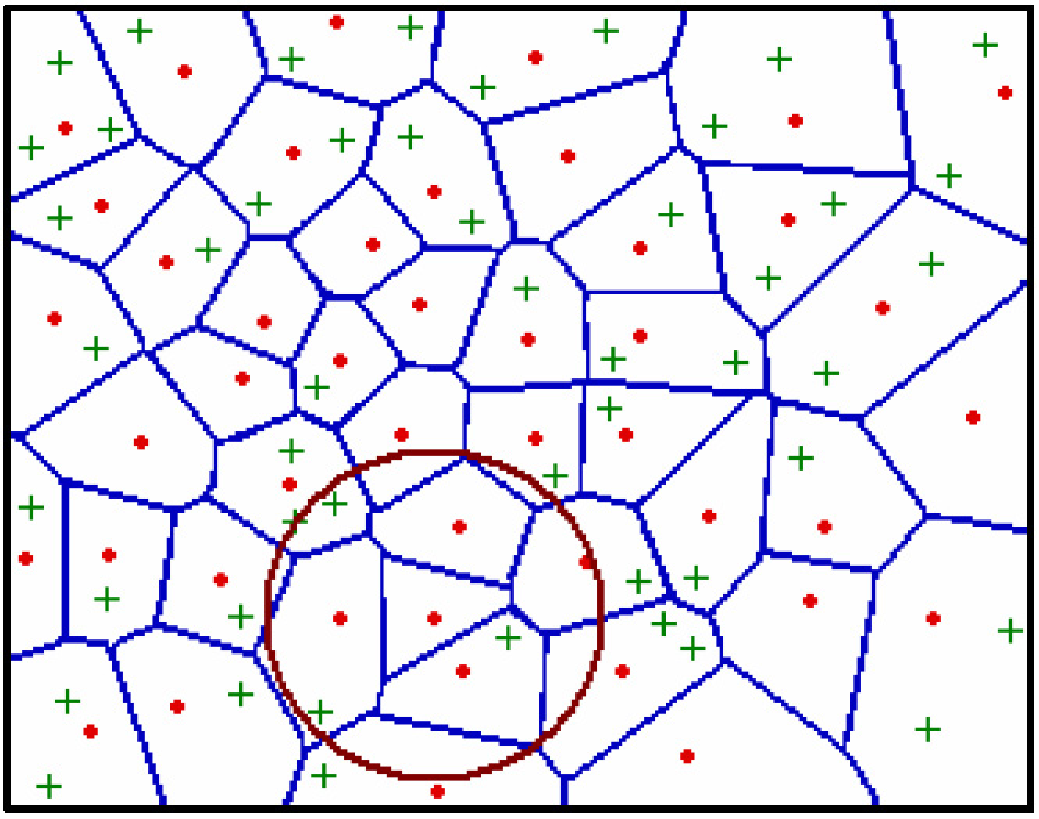
\includegraphics[width=0.4\columnwidth]{voronoi_diagram}
 \caption{Voronoi Diagram \cite{Buyukkaya_voronoi_state_management}}
 \label{fig_voronoi_diagram}
\end{figure}
%
Given a set of points, the Voronoi diagram of the set of points is the partition of the plane, which associates a region around every point in such a
way that all other points contained in the region are closer to the centre point than any other point in the set. Figure \ref{fig_voronoi_diagram}
shows a Voronoi diagram, where the lines define the region boundaries, the dots define the players, which make up the set of points for which the
diagram was calculated, the plus signs represent mutable objects and the circle represents the AoI of a central point in the set.

For the Voronoi approaches, described in more detail in Section \ref{distance_based_existing_archs}, a node controls and hosts all objects within its
Voronoi region. The reasoning is that there is a high probability that the player closest to the object is also the player using the object. Examples
of this are where a player is trading or fighting with an NPC.

\subsection{Responsiveness}

%Distance-based - issues
An issue with the above reasoning is that multiple nodes are usually interacting with a single object. The examples of the NPC monster and trader are
again relevant. Usually many players interact with a trader NPC and usually players attack monster NPCs in groups.

Multiple player interactions are, however, not as big an issue as others have suggested \cite{Fan_deisgn_issues_p2p}. In the best case, the object
being used by a player is also hosted on that player's node. If another player requires use of a remotely hosted object, that player may still
interact with the object, where the host node is now acting as a server to that player. This means that every player hosting an object becomes a
server for that object. In the case where a player interacts with an object hosted locally, there is no object latency. In the case where a player
accesses a remotely hosted object, there is only one hop latency, the same as with a C/S or super peer application.

Issues with this approach stem from the fact the players are constantly moving. When players move, the objects in their regions change. Objects,
therefore, have to be constantly handed over from one peer to another, which might cause significant network traffic. An object in transit might also
delay interaction with that object. Because object transfer introduces overhead into the system, how regularly an object has to be transferred and
whether the number of transferrals produce sufficiently low overhead to implement a real-time game, still have to be investigated.

Voronoi-based storage schemes also become unresponsive when communications are no longer between neighbours, but between two arbitrary nodes in the
Voronoi overlay. When such communications occur, the average required time to route a message is $\OO{N^{1/2}}$ for a two-dimensional configuration.
Advancements have been made that suggest augmenting the Voronoi overlay with additional links to far off nodes to create a small world network. This
reduces the average routing time to $\OO{\log{(N)}}$, the same as for overlay storage \cite{Steiner_voronoi_shortcuts}.

\subsection{Reliability}

Reliability, because of network churn, is still an issue. Nodes will leave the network whenever a player stops playing the game, which makes it a
common occurrence. When nodes leave the network, the objects that are stored on that node should still be accessible to other players. This will
require transferring all objects contained in the leaving node to another object, still present in the network. No papers have yet dealt with the
issue of reliability in a distance-based storage network.

The same solution that is used for overlay storage, namely the presence of redundant peers, might also be implemented for distance storage. Another
structured overlay might be used to implement this redundancy in exactly the same way it is done with hybrid storage mentioned in Section
\ref{hybrid_storage_reliability}.

\subsection{Security}
\label{distance_based_storage_security}

The main issue with the distance based scheme is security. Nodes that have the most interest in an object also have the most interest to manipulate
that object in ways inconsistent with the game rules. When objects are hosted on nodes that have the most interest in them, there will be a strong
drive to try and manipulate these objects. Because these modification are all local, it is also not possible to log the alterations and detect
cheating. Means by which local objects can be secured have to be found or distance based algorithms with quorum need to be investigated.

This security issue is similar to that of super peer storage, in that local data can be accessed, thus circumventing the certification system. With
this circumvention, the objectives of authentication, authorisation, confidentiality, trust, privacy and identity management are all compromised.

\subsection{Fairness}

Distance-based storage is relatively fair as all objects are distributed amongst all nodes. Where the system becomes somewhat unfair is when a node
is nearest to a large number of objects. For Voronoi regioning approaches, this is when a peer's Voronoi region contains many more objects than the
average number of objects hosted by other peers. This might not be a major issue, depending on how long the objects have to be hosted on the
overloaded peer. This will depend on the movement of the overloaded peer as well as that of neighbouring peers. The use of aggregators as a proposed
solution to this problem is discussed in Section \ref{distance_based_existing_archs}.

\subsection{Existing architectures}
\label{distance_based_existing_archs}

%Colyseus, 2006
Bharambe et al. created the Colyseus architecture in 2006 \cite{colyseus_distance_based}. The architecture is designed to support First Person
Shooter (FPS) games and implemented to function with Quake II. Mutable game objects are stored on the peer that is nearest to the object in the game
world. An ``object placer'' component is mentioned, but the details of the placement algorithm are left for future work. The architecture also does
not implement non-volatile state persistency, since this is not required for normal FPS games, where object states need only exist to the end of a
round and where players generally do not leave before the end of the round. This means that object states are only stored in primary memory, until
the end of a game round.

%Solipsis, 2008
The Solipsis architecture was created by Frey et al. in 2008 \cite{solipsis}. The architecture uses Voronoi diagrams to create virtual regions.
Stationary objects are maintained by site nodes until a player picks up an object. When an object is picked up, control of that object is transferred
to the player that picked up the object. The Solipsis architecture focusses on distributed physics computation and when a player gains control of an
object, that player is responsible for the object's physics computations. That player should also save all object state until a new player takes the
object, at which time control is transferred to her. Control can also be transferred back to a site node if an object remains stationary for some
time.

What differentiates the Solipsis distance-based storage from the other architectures presented in this section, is that object states are only
handled by peers as long as those peers directly use an object. At other times, those objects are handled by site nodes. This differs from other
distance-based storage techniques, where all objects that are nearest to a player in the virtual world are controlled by that player.

%Buyukkaya and Abdallah, 2008 and Hu et al., 2008
In 2008, papers were published by Buyukkaya and Abdallah \cite{Buyukkaya_voronoi_state_management}, and Hu et al. \cite{Hu_voronoi_IM}, proposing to
use Voronoi diagrams \cite{voronoi_diagrams_survey} to implement distance-based storage. Voronoi state management schemes host the mutable objects on
the peer in which region the object exists. As peers move around in the virtual world, the Voronoi diagram has to be constantly recalculated and
objects have to be moved to new owner peers as the regions in which they fall change. The significant advantage of the Voronoi approach is that peers
only require connections with their neighbours, and peers within their AoI.

A thesis by Chang also describes the Voronoi approach in more detail and how to achieve game state consistency amongst all nodes in a Voronoi network
\cite{Chang_Voronoi_state_management_masters}. What distinguishes this work from the others is the implementation of a load balancing mechanism. When
peers get overloaded, another, more powerful peer is chosen as an Aggregator. The Aggregator assumes responsibility for a larger area that
encompasses multiple peers. This scheme will reduce the load on peers with minimal resources, but it is uncertain how this would reduce load when
peers with an average number of resources in an area become overloaded.

The works by Buyukkaya and Abdallah, Hu et al., and Chang form part of the VAST project, which is being created to be a fully functional P2P overlay
architecture, using Voronoi diagrams as its basis \cite{VAST}. The reason why state persistency in Voronoi-based P2P MMVEs architectures are mostly
distance-based approaches, is because the Voronoi diagram immediately identifies which objects are closest to a particular peer, and therefore, which
objects that peer has to host. Architectures not making use of Voronoi diagrams still require some other mechanism to identify which objects which
peers should host.

\section{Summary and recommendations}
\label{recommendations}

Supper peer storage can be seen as a C/S type storage implementation, where every region has a super peer that stores all data for that region.
Overlay storage is a fully distributed, P2P approach to storage, where every node stores data as part of a P2P overlay network. Hybrid region based
storage combines super peer and overlay storage to improve the overall storage performance. Distance based storage is a different paradigm that
stores game objects on the nearest node to that game object. This type of storage is usually characterised by the use of Voronoi diagrams to
determine which nodes are nearest to which objects.

Super peer storage is characterised by its high level of responsiveness and ease of implementation. Overlay storage is characterised by its high
level of fairness and reliability. Hybrid region-based storage combines the two previous schemes and has high levels of reliability and
responsiveness. Distance based storage is also very responsive and can be made both reliable and fair.

Security is still an issue for all storage types. Super peer storage has the issues that are usually present in a centralised system, namely low
fairness, security and also not being reliable and not resistant to failure. The main issue with overlay storage is its unresponsiveness, because of
the routing delay in the P2P overlay. Hybrid storage suffers from the disadvantages of super peer storage, namely low fairness and security, due to
all files still stored on super peers. The main issue of distance based storage is security, because players that have the most incentive to alter
object states own those objects.

The different storage types vary greatly in implementation complexity as also shown in Table \ref{tab_storage}. The simplest type of storage to use
is super peer storage, but because of the many issues present, this is not recommended. Only when one is sure that the super peers will not be
overloaded should this storage method be used. There might still be some customers who are unhappy that a few have to serve data to the many.

No recent mention could be found of researchers implementing super peer storage for P2P MMVEs. This could mean that there has been very little
evolution in super peer storage and that super peer storage is currently less mature than other storage schemes. Super peer storage might still be
used for small independent casual games, such as online board games, where a group of friends can implicitly trust each other or where the risk of
cheating is at a minimum. The reason why this storage method is recommended for games from independent developers, is because the scheme is easy to
implement and will not require many resources when used for small games.

For developers who are looking for a simple yet fairly robust storage system to start using in their project, overlay storage is recommended. Overlay
storage can be used for games that do not require low latency data access and would allow for lazy updating of the database. These games will be
lightweight casual and social games. But, depending on the game implementation itself, this storage type might also be used for smaller hardcore
games. Overlay storage will place some restrictions on certain game mechanics, but it is possible that games could be designed around these
restrictions. The primary restriction being that data cannot be immediately retrieved or stored from or to storage.

Examples of overlay storage types that might be used are: PAST, Freenet and Oceanstore and any other overlay storage that is based on a DHT overlay.
Storage based on DHT overlays is still a viable research field and future implementations will improve on the present systems.

Hybrid region-based storage has all the advantages of super peer storage, but with the additional reliability of overlay storage. For this reason, it
is recommended that any game presently requiring high levels of reliability and responsiveness use hybrid storage, instead of super peer or overlay
storage. This storage type currently seems to be the only type applicable to games that require responsive and reliable storage.

%Implementation complexity of hybrid storage
That said, no existing implementations could be found that implement this type of storage for public use. The consequence is that someone who wishes
to use this storage will mostly have to implement it. This can be done by starting out with super peer storage and using a publicly available overlay
storage to augment the super peer storage.

Distance based storage is still fairly immature, but shows a lot of promise. No publicly available implementation could be found for this type of
storage. Where this type of storage was used, it was explained as distance based storage, but most of the details were left out. This storage is,
therefore, not a candidate as a storage technique for developers that are merely looking for a storage system to use presently. This type of storage
does, however, provide a lot of opportunities for research.

\section{Conclusion}
\label{conclusion}

\subsection{Summary}
%Paper summary
After providing an overview of the classic C/S and C/MS state persistency techniques, this survey classified P2P MMVE state persistency techniques
into super peer based, overlay based, distance based and hybrid storage. The advantages and disadvantages of each method were discussed after
identifying key challenges that state persistency techniques have to solve. These challenges are: Reliability, Security, Fairness and Responsiveness.

We conclude that there exists no single state persistency architecture, currently in use, that is suited to P2P MMVEs. None of the storage techniques
reviewed meet the requirements of a real-time distributed application, such as an MMVE. What is required is a state persistency architecture,
specifically geared towards data persistency in P2P MMVEs, that meet all the challenges of the application.

%Reason for paper
This survey was written, because of an identified need for a concise summary of the field of P2P MMVE game state persistency. Many techniques used in
the past were used because of the ease with which they could be integrated into a P2P MMVE. The purpose of this survey is to identify those
techniques and to stimulate further research, using empirical methods to compare the different storage techniques used.

\subsection{Prospective research directions}
%How to address storage challenges
One of three paths may be followed in order to create a storage type that is suitable to modern hardcore MMVEs. The first would be to take a look at
the deficiencies mentioned in the different storage types and to then improve one of these types. The other path is what was seen with hybrid
storage, where multiple types of storage are combined in order to form a new and improved storage type. The third path would be to create a new
storage type, based on some novel insight into the ways in which games are designed.

%What are some of the challenges of the different storage types
What follows is a discussion on what work is required in order to improve the current storage types and attempts to define the gaps present that
should still be solved by future researchers.

For super peer storage to become viable, a means is required to secure the data stored in the super peers and ensure that no super peer is able to
access the data stored. If this issue is solved, the fairness issue still exists, but might be allowable depending on the type of application.

%Overlay storage - reason
Overlay storage is a popular storage method in the literature. This is believed to be more as a consequence of the use of Scribe \cite{scribe} than
any inherit benefit to P2P MMVEs \cite{past_storage_focus}, \cite{Fan_phd}. The reason for using overlay storage in so many implementations seem to
be merely the availability of PAST, after having already decided to use Scribe. In other words, researchers use Scribe for ALM, Scribe runs on
Pastry, and PAST is then a readily available storage implementation which also runs on Pastry.

The applicability of overlay storage to MMVEs is still unknown and further research is required. This paper showed that while PAST is regularly used
in P2P MMVEs, it is not because of the applicability of PAST to P2P MMVEs.

One type of hybrid storage was investigated in this paper, namely overlay/super peer storage, since this is a hybrid type currently seen in P2P
MMVEs. Other hybrid types should also be investigated, for example a distance based/overlay storage hybrid might improve the reliability of distance
based storage. Multi-tiered storage might also be of interest, where players or areas are grouped in some way. One type of storage might then be
implemented amongst the members of a group, with another storage type implemented over all groups. Such a storage type might improve responsiveness
amongst group members, while adding reliability because of an inter-group backup mechanism.

Distance-based storage still seems immature, with many open questions. Currently, distance-based storage is based on Voronoi diagrams, which seem
promising. But Voronoi diagrams only provide for a means to identify which objects should be under a specific node's control. Object migration, which
will occur frequently in this type of storage should still be addressed. The number of migrations should be kept to a minimum to ensure responsive
access to all stored objects.

The storage is also not yet reliable, but it could be possible to add overlay storage as a backup to the system and thereby add reliability. If
voting techniques can be used to update game state, some of the security issues might also be solved. With these two issues addressed, the high
degree of fairness of distance-based storage makes it an excellent candidate to power the P2P MMVEs of the future.

%Performance comparison of storage
An empirical comparison of the performances of the different storage types is also required. It is believed that the metrics presented in this paper
could provide a common basis to use in comparing the different storage types.

%Need for storage characteristics
Research is still required into the characteristics of data stored by MMVEs. This includes how regularly game objects are stored as well as the sizes
of these objects. It is also expected that different read and write patterns exist for different types of game objects. These patterns should be
explored in order to determine what the required performance is for P2P MMVEs storage mechanisms.

It is recommended that C/S MMVE storage patterns initially be investigated to provide a benchmark of the required storage performance for a mature
MMVEs. The storage patterns for a C/S compared to P2P MMVEs might be different. The storage patterns amongst different MMVEs might also differ
greatly, but for an immature field any data is better than no data.

In conclusion, this paper describes a possible new research field with many open questions still to be answered.

\chapter{Pithos Design}
\label{chp:DESIGN}

The generic state consistency model was presented in Section \ref{generic_event_update_model}. One of the key challenges that still remain was determined to be designing an authoritative storage module specifically tailored to P2P MMVEs. The authoritative storage module identifies in Section \ref{generic_event_update_model} includes the processes of state management and state persistency for the authoritative objects.

We've identified the main requirements of P2P MMVE state management and persistency in Section \ref{key_challenges_cm} as: scalability, reliability, fairness, responsiveness and security. In Chapter \ref{p2p_MMVE_state_persistency} it is argued that none of the current approaches to state persistency satisfy all identified requirements. The focus of this work is on state management and persistency in P2P MMVEs. This chapter proposes a novel design, called Pithos, that satisfies all the identified requirements.

The novelty of Pithos lies in its support for both a responsive and a fair storage system, while also taking into account security aspects
of distributed storage. There are some storage systems that provide responsive or fair storage, but none that provide both. No storage system, designed specifically for P2P MMVEs, have taken security into account.

If Pithos is incorporated into an existing P2P MMVE consistency architecture, it will add the ability to handle both state management and state persistency. The addition of a robust state management and persistency mechanism, specifically designed for P2P MMVEs, will bring us one step closer to the creation of a complete P2P MMVE architecture.
%%%%%%%%%%%%%%%%%%%%%%%%%%%%%%%%%%%%%%%%%%%%%%%%%%%%%%%%%%%%%%%%%%%%%%%

\section{Use cases}
\label{use_cases_goals}

The purpose of Pithos is to allow for efficient object storage and retrieval that satisfies all identified requirements. As is evident from authoritative storage in the flow diagram in Figure \ref{fig_event_update_flowdiagram}, Pithos will interface directly with the VE logic, as well as receive updates from the update generator. For the purposes of this discussion, update generation is assumed to be part of game logic.

\begin{figure}[htbp]
 \centering
 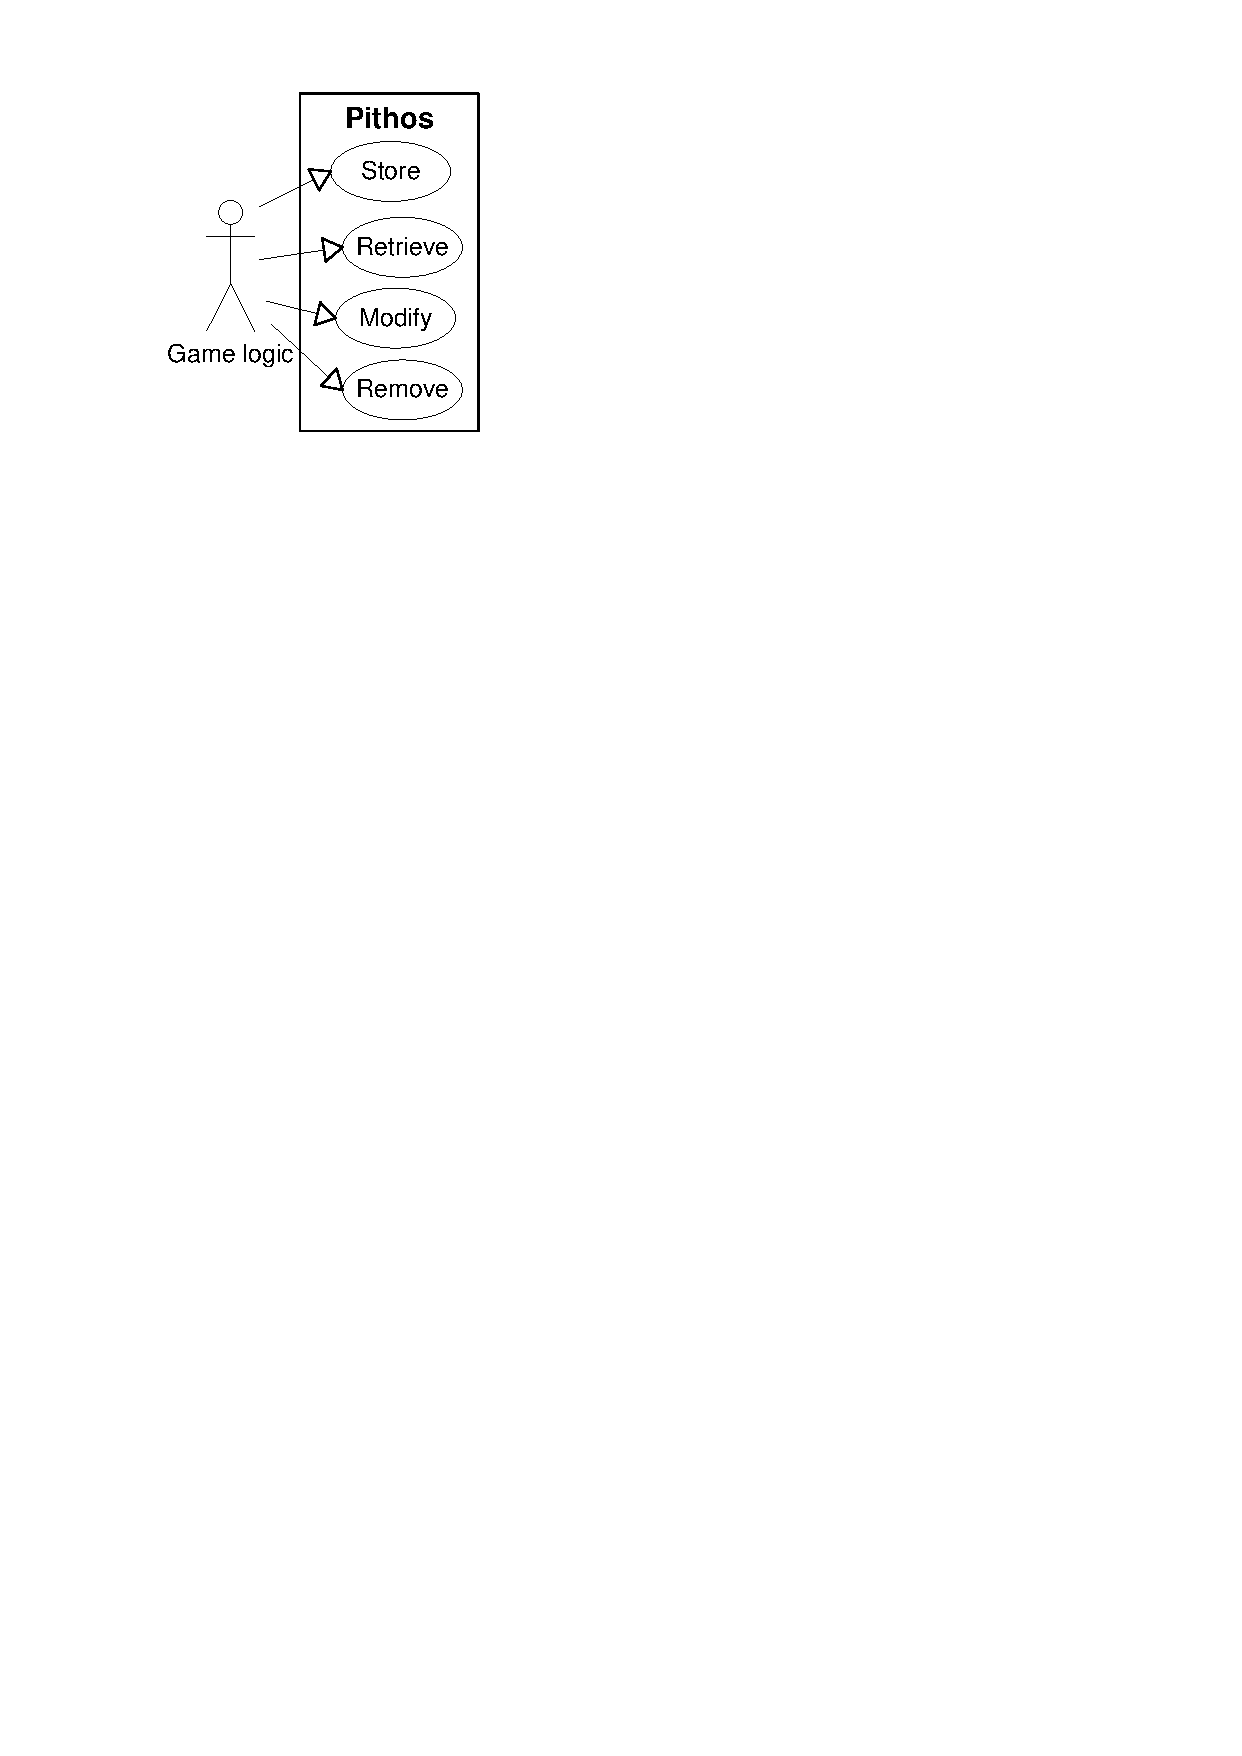
\includegraphics[clip=true, viewport=28mm 223mm 82mm 282mm, width=0.3\textwidth]{pithos_use_case}
 \caption{Use case diagram of Pithos}
 \label{fig_pithos_use_case}
\end{figure}

As shown in the use case diagram in Figure \ref{fig_pithos_use_case}, the VE logic should be able to use Pithos in four ways: store, retrieve, modify and remove. These are the use cases generally required of any storage system.

\subsection{Store}

The VE logic will store data when a new object is added to the VE state. This can happen as a consequence of an event leading to the generation of a new object. An example of this is a rocket firing at a target. This event might generate a missile object to be sent towards the target.

\subsection{Retrieve}
Object retrieval will be required every time an event is received. The VE logic will retrieve the object state from memory, which is part of state management. Object states, other than the one being altered, might also be required by the logic to determine the effect an event will have, as discussed in Section \ref{event_logic_update}.

\subsection{Modify}
Object modification occurs every time an object update is generated. An object update, by definition, required a modification of the object state.

\subsection{Remove}
Object removal might also be required to save storage space, although this is not essential to the correct functioning of the storage system.

\section{Designing for the storage requirements}

Pithos is designed to fulfill all use case requirements as well as the storage requirements for P2P MMVE storage architectures as set out in Section \ref{key_challenges_cm}. To achieve both these goals, an architecture was first designed to fulfill all the storage requirements and the use case requirements were then implemented on the designed network.

The inspiration for Pithos come from two observations:
%
\begin{enumerate}
  \item One can combine multiple storage models and arrive at a model which possesses fewer disadvantages than any of the models used.
  \item Responsiveness is greatly increased in a fully distributed model, where there is no intermediate server that relays all information.
\end{enumerate}

Fully distributed architectures are, however, not scalable because the number of messages scaling by $O(N^2)$, where $N$ is the number of nodes in the network.

This section will describe how the design of Pithos satisfies the identified storage requirements. For each of the requirements of responsiveness, reliability, security and fairness, the design decisions made to achieve the specific requirement will discussed. Some design decisions satisfy multiple requirements, therefore different requirements might discuss the same design decision, with a focus on how the decision satisfies the specific requirement.

\subsection{Responsiveness}

In Pithos, responsiveness is achieved by grouping players into fully connected groups, using group-based distance-based storage to distribute objects and using replication to enable the parallel retrieval of objects.

\subsubsection{Group storage}

In a fully connected network, where all nodes are connected to all other nodes, every node is one hop away from every other node. This solution is, however not scalable. In order to achieve a scalable single hop architecture, it was decided to group users in the virtual world. User groups are then fully connected, which allows for highly responsive group interactions. Group sizes are smaller than the overall network size and allows for the fully connected groups to remain scalable.

In virtual worlds, users already group themselves into explicit groups, including questing groups, raid groups and guilds. In Section 3.1 of \cite{varvello_phd}, it was found that most users in Second Life form small groups.  Implicit groups are also formed by flocking, where multiple users congregate in areas of the virtual environment that are of interest to them \cite{flocking}.

\subsubsection{Distance-based storage}
Grouping users is not sufficient to achieve a responsive system. Users should also require data stored in the group more than data stored outside the group. To this end, distance based storage is used on a group level. This means that objects are stored in the group that is closest to them. The assumption is that users interact more with objects that are closer to them and, therefore, have more interest in closer objects. If a user has interest in a far off object, she will likely move closer to that object.

\subsubsection{Replication}

Multiple copies of an object are stored. Replication improves responsiveness, because multiple copies of an object may be requested in parallel and the object that arrives fastest is used.

\subsection{Reliability}

Reliability is achieved by storing all objects on overlay storage (DHT), in addition to group storage, replicating all stored objects and repairing object replicas as they are removed due to network churn.

\subsubsection{Overlay storage}
Distance-based group storage attempts to maximize the number of requests for objects within a group. The number of actual intra-group vs. inter-group requests will still depend on the grouping algorithm and it might not be possible to ensure that all requests remain in the group.

In order for peers to be able to requests objects stored in other groups, overlay storage is used. Peers belong to both a group and the overlay. Peers can therefore request data from the group and from the overlay. Overlay storage adds reliability by ensuring that out-of-group object request can also be served.

Every retrieve request is requested from both the group and the overlay storage. If any of the storage types fail, the other might still succeed, adding reliability.

\subsubsection{Replication}

Replication allows for multiple peers to leave the network before an object becomes unavailable, improving reliability. Because of network churn, replication is essential to ensuring objects survive network churn. If only a single object is stored, a node unexpectedly leaving the network destroyers an object. There is no chance of an object being recovered when no replicas are used.

\subsubsection{Repair}

Repair further improves reliability by maintaining object replica numbers. When it is discovered that a peer has left the network, peers storing the objects of the peer that left can replicate those objects, thereby maintaining the number of replicas.

A system only using replication's object numbers will steadily decline from the time an object was stored. A system using repair can replace missing replicas, ensuring long term object survivability.

\subsection{Security}

Security cannot exist in a single system layer and has to be ensured on multiple layers, as discussed in Section \ref{characteristics_security}. Some security concepts implemented in Pithos are the use of a certification authority, replication and quorum.

\subsubsection{Certification}

A difference between Pithos and other P2P systems is that it requires all peers to be uniquely identifiable. A main requirement of classic P2P storage architectures is that peers remain anonymous to ensure user privacy. In Pithos, all users are unique identifiable. An object records which user created it and which users modified it. This allows for the identification of users that maliciously alter objects.

\subsubsection{Replication}

Storing multiple replicas attempts to limit the effect that a malicious user might have on the storage system. If a malicious user altered an object, the original object is still stored on multiple peers.

\subsubsection{Quorum}

When security is a concern, multiple parallel retrieval requests can be performed. A quorum mechanism is then used at the receiving peer to compare the different received objects. The object that is returned by most of the peers is then considered the correct object. A peer modifying an object has no effect on the system, since the receiving peer selects the object returned by the other peers.

\subsection{Fairness}

Fairness is achieved by using overlay storage and group storage.

\subsubsection{Group storage}

Objects are uniformly distributed on group peers, ensuring that all group peers share the load of group objects stored.

\subsubsection{Overlay storage}

Overlay storage maps objects and peers to the same uniform key space and stores an object on a peer that is the closest match for the object's key. This uniformly random mapping ensures a uniform distribution of objects in the overlay.

\section{Key modules and mechanisms}
\label{key_modules_mechs}

\begin{figure}[htbp]
 \centering
 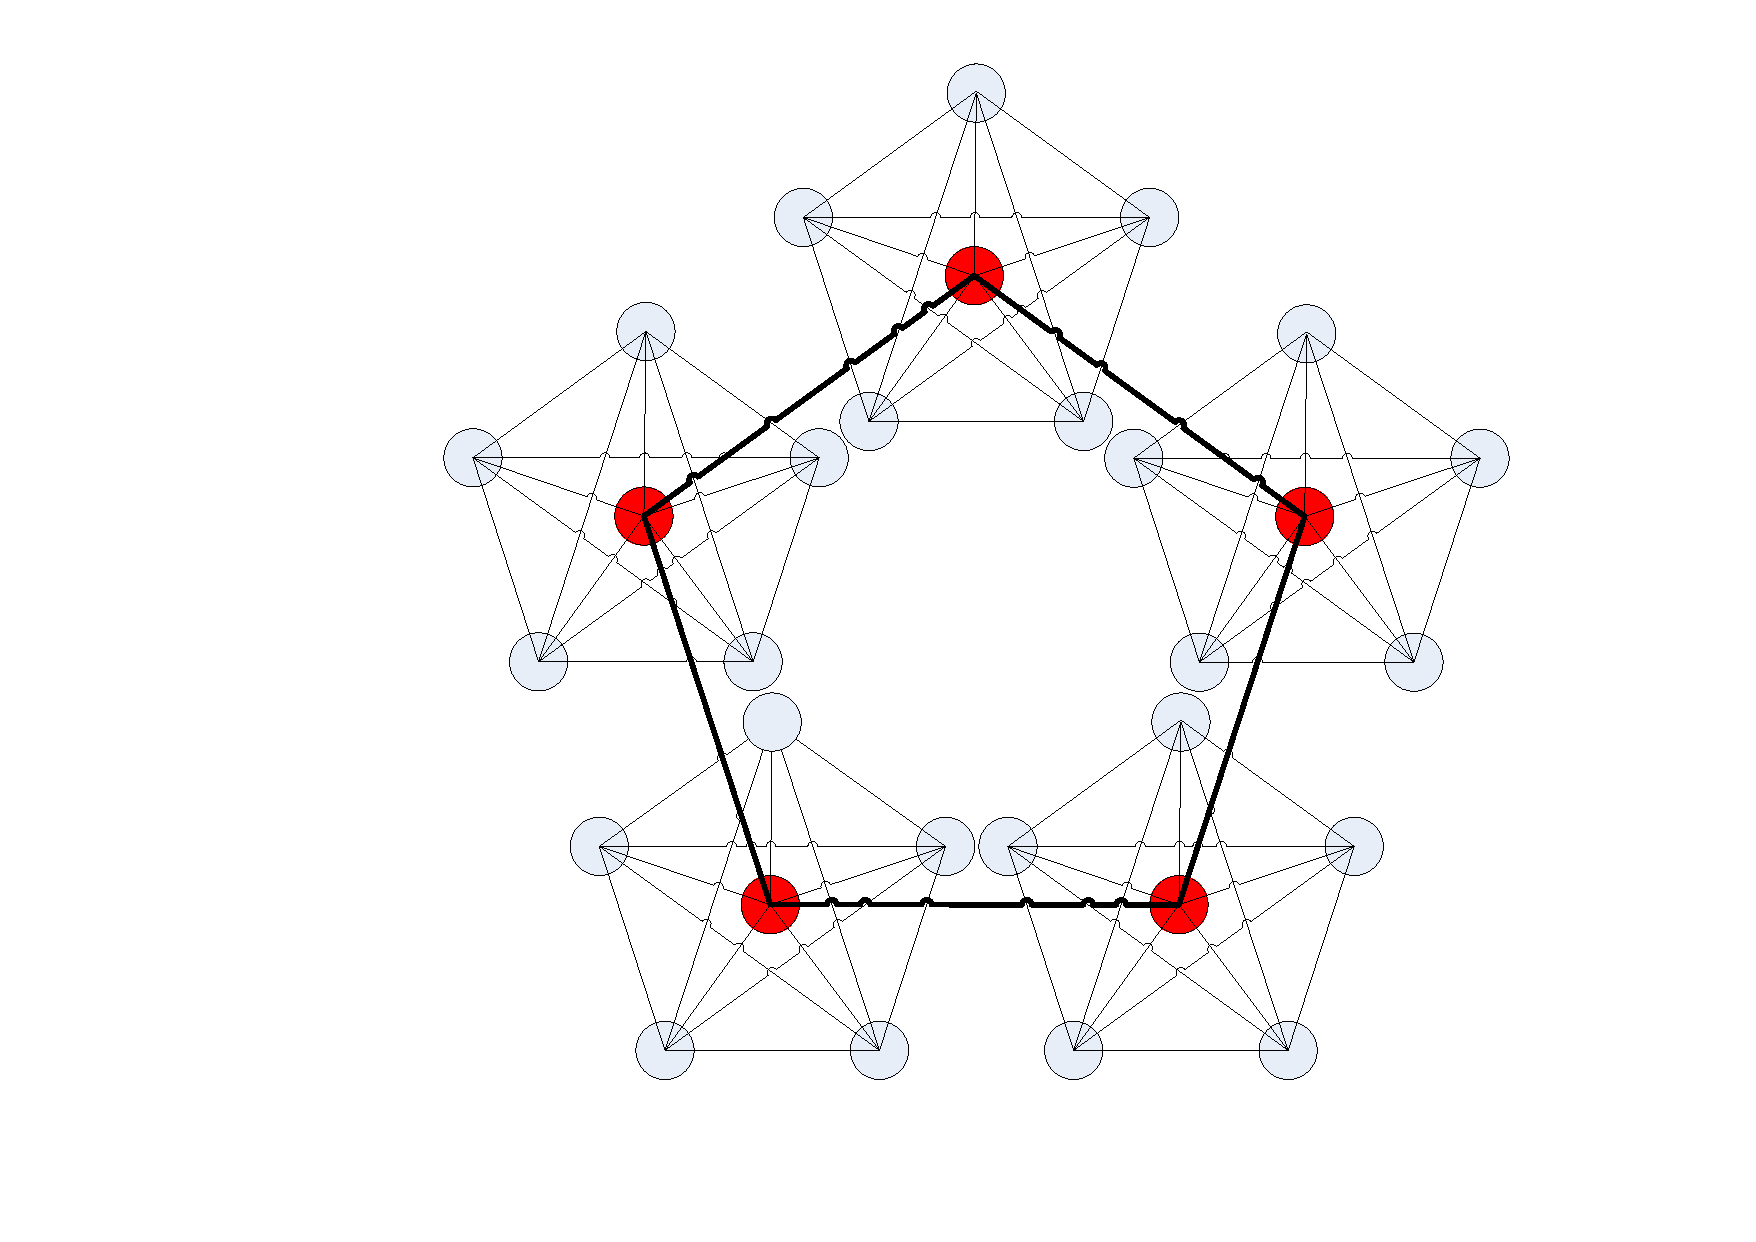
\includegraphics[clip=true, viewport=7.5cm 2.5cm 26cm 20cm, width=0.7\columnwidth]{CDHT_layout}
 \caption{Layout of the Pithos storage architecture}
 \label{fig_pithos}
\end{figure}
%
Figure \ref{fig_pithos} shows the Pithos architecture. The figure shows groups of fully connected peers (light blue and dark red), where all groups are connected to each other in an P2P overlay through super peers (red).

Pithos groups peers to form a two tiered storage model. The first tier is a storage model at group level (group storage) and the second is a storage model over all groups (overlay storage).

Pithos can be considered as a multi-tiered structured overlay, with group storage an implementation of an $O(1)$ overlay and overlay storage an implementation of an $O(\log (N))$ overlay.

When referring to state management and persistency as defined in Section \ref{management_persistency_def}, Pithos is designed to serve both requirements. Group storage is designed for state management and overlay storage for state persistency. Since state persistency does not require responsive storage, the overlay section of Pithos is well suited to this task, while group storage, with its high responsiveness is well suited to state management.

\subsection{Group storage}

If group storage is considered an $O(1)$ structured overlay, it requires all features mentioned in Section \ref{structured_overlay_features}: geometry, routing functionality, a join mechanism, a leave mechanism and bootstrapping.

On a network level, group storage consists out of three node types: super peers, peers and a directory server. It is possible for a single Pithos terminal to be both a peer and a super peer.

\subsubsection{Geometry and routing}

The geometry is fully connected and routing in such a geometry is trivial. A peer's routing table contains a list of all peers in the group. To route a message to a destination peer, the peer address is retrieved from the routing table and a message is directly sent to that peer.

\subsubsection{Super peers and peers}

In group storage, peers handle requests from the higher application layers. Peers also represent users in group storage, which means that peers are the originators of all store, retrieve, modify and remove requests from a group perspective. The peers themselves receive those requests from the higher layer.

Super peers are responsible for representing a group and managing group membership. Super peers also implement object repair.

\subsubsection{Join mechanism and bootstrapping}
\label{join_mechanism_design}

The directory server places joining peers into groups represented by super peers. The first task of a Pithos peer is to join the network and a group. This is done using the directory server, which possesses a static IP address and port that is known to every new peer and super peer.

\begin{figure}[htbp]
 \centering
 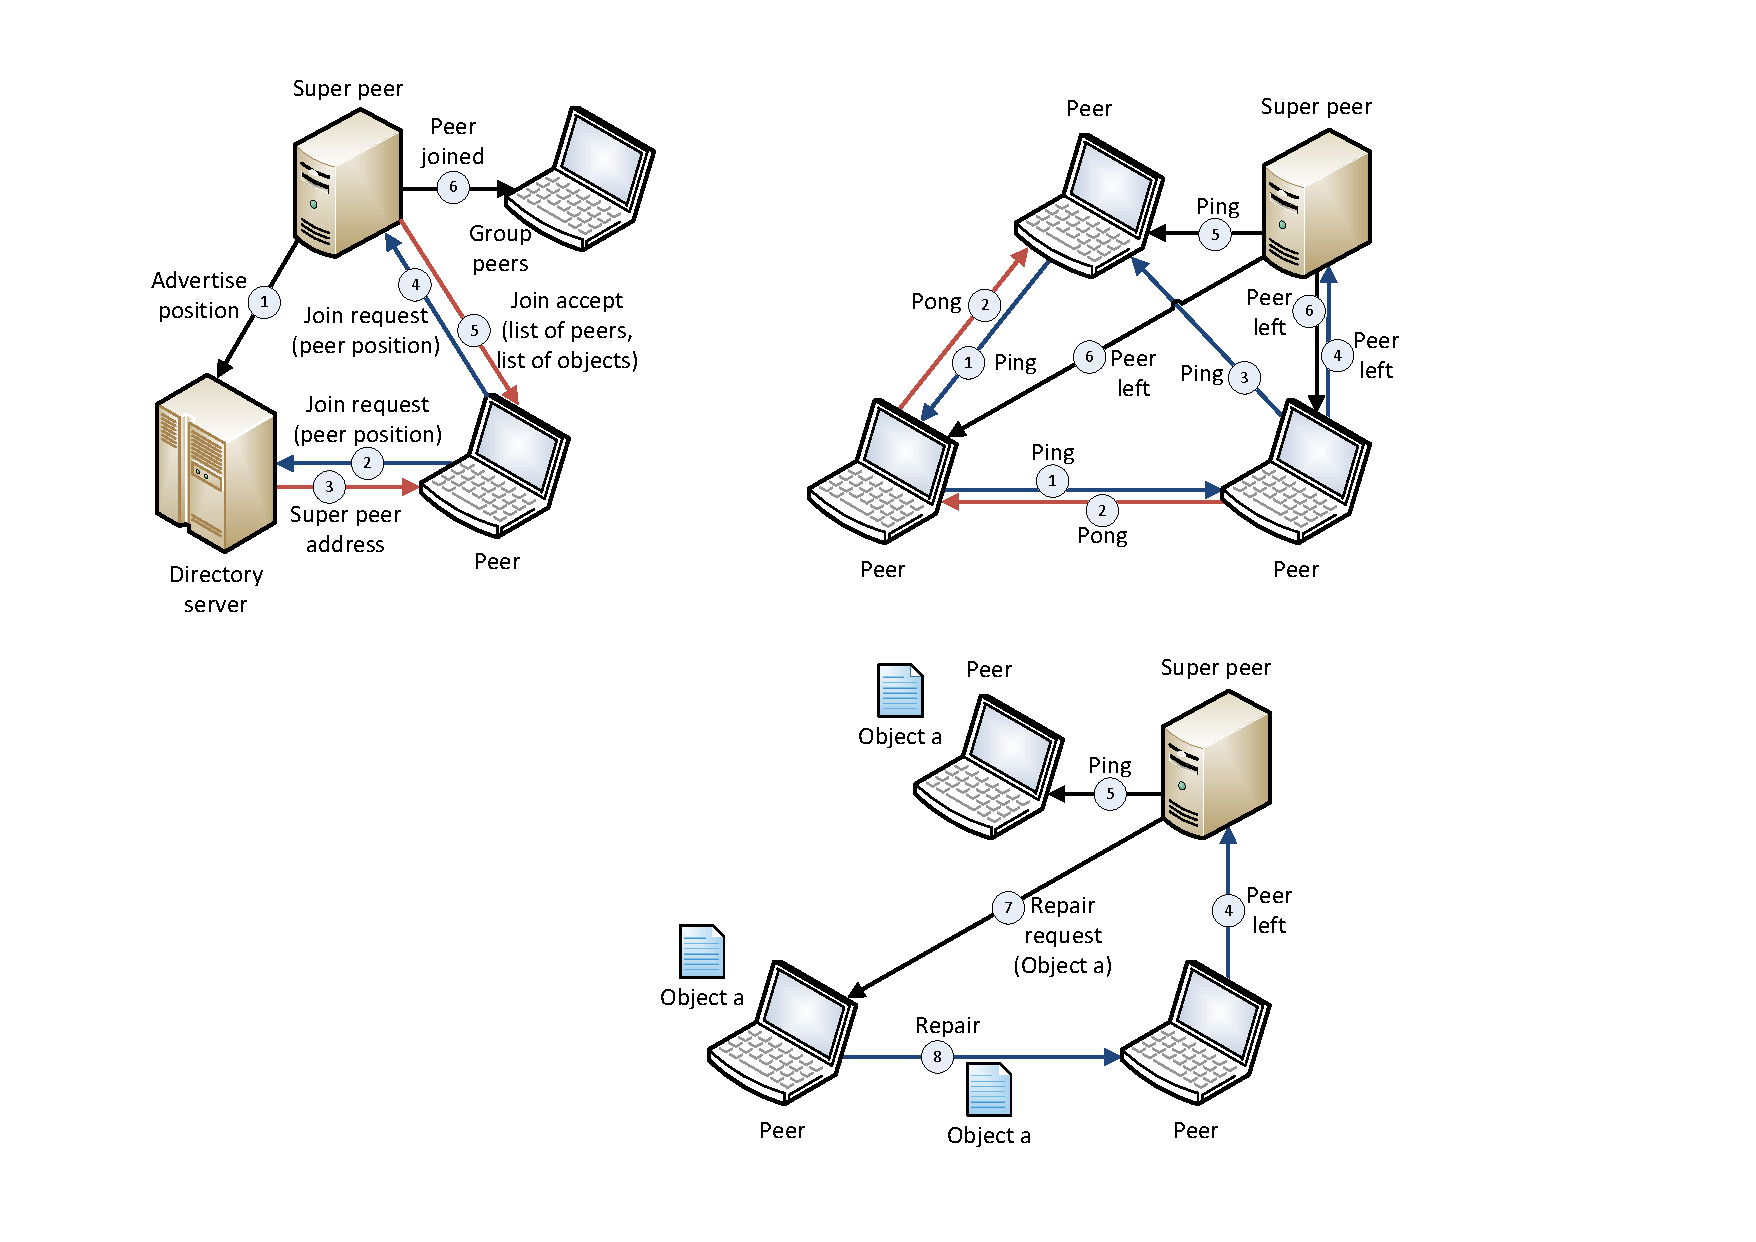
\includegraphics[clip=true, viewport=15mm 105mm 115mm 199mm, width=0.7\columnwidth]{Pithos_mechanisms}
 \caption{Pithos group join mechanism}
 \label{fig_pithos_join}
\end{figure}
%
With reference to Figure \ref{fig_pithos_join}, the join and bootstrapping mechanism works as follows:
%
\begin{enumerate}
\item Whenever a super peer is created or potentially selected, it advertises its information with the directory server. This information includes its IP address, port and location of the super peer.

\item When a peer wishes to join the network, it sends its current location to the directory server.

\item  The directory server then responds with the address of a super peer, representing an initial group which the peer can join.

\item The joining peer then sends the same type of join request to the supplied super peer address.

\item If the super peer accepts the joining peer, it sends that peer a list of all peers currently in the group, as well as a list of objects currently available in the group.

\item The super peer also informs all other group peers of the newly joined peer.
\end{enumerate}

The super peer can elect to accept or reject the joining peer. This extra step is intended to prevent groups from becoming overloaded. The super peer can supply an alternative address for the joining peer to contact. This extra step is also intended to compensate for the movement of super peers. If a super peer moves, and by the time a joining peer contacts a super peer there is another super peer in closer range, the super peer receiving the join request can supply the joining peer with the address of the closer super peer.

\subsubsection{Leave mechanism}
\label{leave_design}

If a peer leaves the network unexpectedly, it will not have the opportunity to inform its group. With no mechanism to detect a peer unexpectedly leaving, group inconsistency will occur. The peer that left might be selected to store an object or might be required to provide an object from storage. These requests will all fail.

\begin{figure}[htbp]
 \centering
 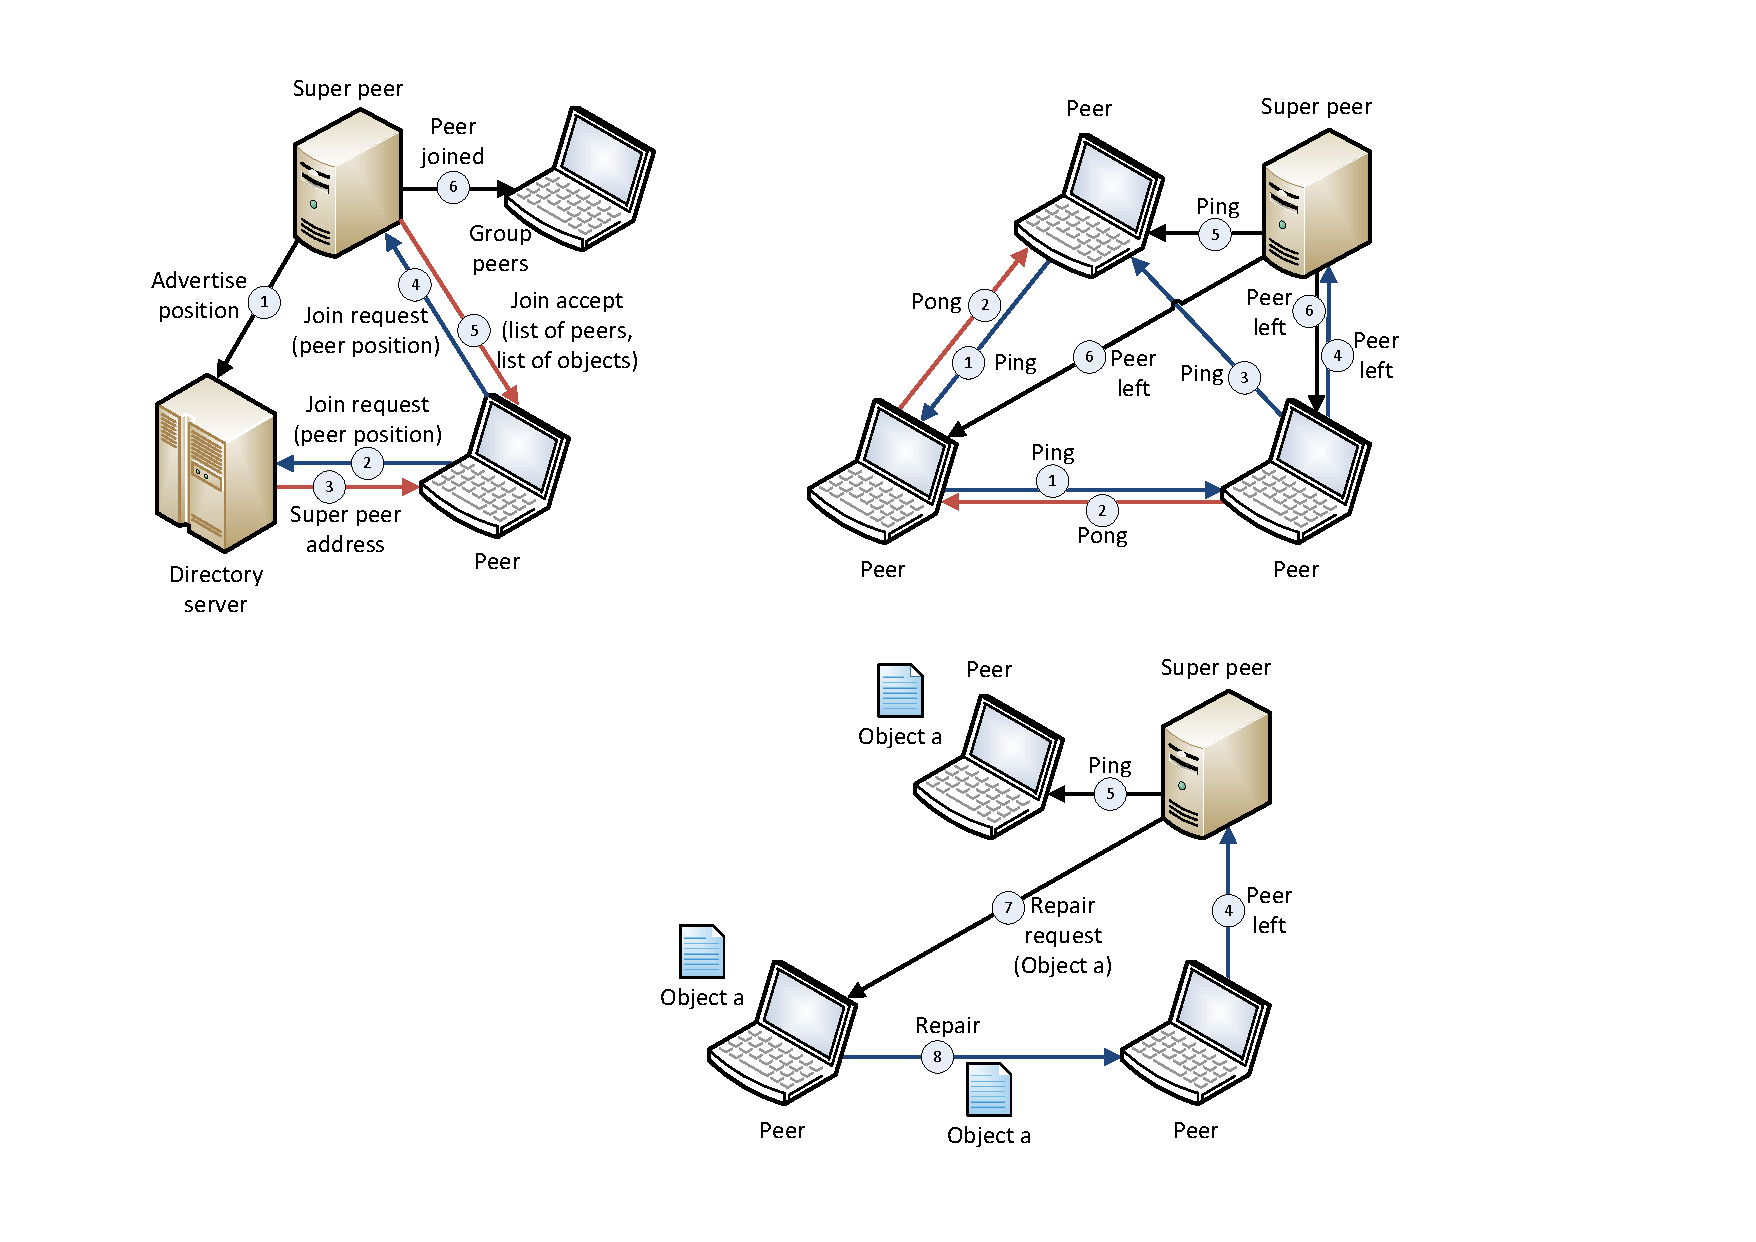
\includegraphics[clip=true, viewport=135mm 110mm 242mm 196mm, width=0.7\columnwidth]{Pithos_mechanisms}
 \caption{Pithos group leave mechanism}
 \label{fig_pithos_leave}
\end{figure}

In Pithos, two methods exist to ensure group consistency and handle peers leaving the group. The first method, shown in Figure \ref{fig_pithos_leave}, uses periodic keep-alive messages as follows:
%
\begin{enumerate}
\item At regular intervals, each group peer uniformly randomly selects another peer in the group to send a keep-alive (Ping) message to.

\item If a peer received a keep-alive message, it responds with an acknowledge (Pong) message.

\item A peer that does not respond with an acknowledge message within a sufficiently large amount of time is considered to have left the network.

\item The originating peer of the keep alive message informs the super peer that the target of the keep-alive message is thought to have left the group.

\item The super peer then also sends a keep-alive message to the target peer, to ensure that there isn't some communications issue between the two group peers and the target peer has actually left the network.

\item If the target peer does not respond to the super peer, the super peer informs all group peers that the target peer has left the group.
\end{enumerate}

The super peer verifies that the peer has left, because by design the super peer is selected to be the most available peer in the group on the network. The super peer does not transmit all keep-alive messages in order to prevent overloading of the super peer.

It is accepted that not all group peers might receive keep-alive messages every round, because of the random selection mechanisms, but this is not required. Only that in a sufficiently few number of keep-alive intervals, the peer is found to have left.

The second mechanism uses requests to identify peers that have left the group. Whenever a request is sent to another peer, a timeout is also started. If a peer does not respond to a request within a given amount of time, the same leave mechanism will be activated has the target peer not responded to a keep-alive message.

It should be noted that either of these methods are sufficient to ensure group consistency over some time period, but using both minimises the time it takes to detect a peer leaving the group.

For graceful group leaves, the same leave mechanisms as used in group migration is employed.

\subsubsection{Migration}
\label{migration_design}

Users will constantly being moving in the virtual environment, leading to changes in position. These position changes may lead to users moving from one group to another. It is imperative that all objects stored in Pithos remain available even with users traversing groups.

As users move around in the virtual world, Pithos queries the directory server with the new positions, using the same mechanism described for joining a group in Section \ref{join_mechanism_design}. The peer then receives a new super peer address from the directory server, if this address is different from the address of the currently known super peer. When a new address is received, Pithos initiates group migration.

Group migration involves informing the group that the peer is leaving, clearing all statistics and initiating the group join mechanism. Informing the group that the peer is leaving ensures that this peer will not be picked for any storage or retrieval requests, while the group is unaware that the peer has left. If this is not done, the group will only know that a peer has left after a timeout for a request to the peer expires, which reduces request success rates.

\subsubsection{Ledgers and object stores}

The previous sections have focussed on group storage, purely as an $O(1)$ structured overlay. To enable the storage of objects within the group, an objects store is also required, as well as a way to track which objects are stored on which peers and conversely, which peers contain which objects.

Each peer in the group contains a local authoritative object store, containing all objects stored on the peer by group storage.

Each peer and super peer in the network contain a group ledger to keep track of which objects are stored on which peers. The group ledger is required whenever an object is retrieved within the group to know from which peer an object can be requested. The ledger is also used by the super peer, to determine which objects should be repaired.

\subsubsection{Grouping}
\label{grouping_design}

In order for Pithos to build group, a clustering mechanism is required. There already exists a wealth of clustering algorithms in literature and a few will be reviewed here.

\emph{Distributed peer clustering techniques}: use the distance between users in the virtual environment to dynamically group players. The main idea of flocking is that players move around in groups, rather than randomly on their own. It is desirable that user density within groups should remain constant, because a fully distributed architecture is not scalable. This means that groups should merge or split as the user density within them change. It might also be required to have mobile groups, where a group has a velocity as well as a position, to be able to uniquely identify groups, even with players joining and leaving and the group moving through the virtual world.

Affinity propagation clusters nodes using a similarity matrix to find similar nodes \cite{affinity_propagation}. The similarity matrix may contain user positions. In this case, affinity propagation will group nodes depending on their location in a virtual world. This algorithm might be well suited to P2P applications, since it is a distributed clustering algorithm based on message passing.

\emph{Dynamic regioning}: divides the virtual world into regions that can be resized or further divided to maintain constant player densities across regions. SOSPS \cite{self_organising_sps_post} creates dynamic regions based on a Voronoi overlay network \cite{voronoi_diagrams_survey}. Near constant user density is achieved by increasing and decreasing the area sizes. This system is based on VON, a distributed Voronoi overlay network designed for MMVEs \cite{VON_VAST}.

Clustering is also used in mobile ad-hoc networks (MANETs) for routing purposes. Mobile-aware clustering algorithms used in MANETs, might also be applicable to P2P MMVEs \cite{clustering_survey}. Mobile-aware clustering uses relative velocities of mobile nodes to define clusters containing nodes with low relative velocity to each other.

Any of the above mentioned techniques might be used to achieve distributed clustering in P2P MMVEs. The focus of this work is, however, not on developing a novel clustering algorithm for P2P MMVEs.

\subsubsection{Distance-based storage}
\label{distance_based_design}

For Pithos to succeed as an MMVE storage architecture, intra-group data requests should be preferred to inter-group data requests. This requirement, combined with the fact that the grouping algorithm geographically groups players in the virtual world, lends Pithos to a storage system based on distance-based storage. Similar to interest management, the assumption is that players have a limited area of interest and require interaction with a limited number of objects within range.

Distance-based storage is implemented on a group level rather than an individual level, which means that objects are stored on the nearest group of players, rather than the nearest user. It is assumed that such an approach will alleviate the security and reliability challenges present in distance-based storage \cite{gilmore_p2p_mmog_state_persistency}.

With group-based distance-based storage, it is assumed that because peers now store objects closest to the group, the objects that they are interested in will most likely be stored within their own group. Therefore, most data requests should be intra-group requests. The overlay storage component ensures that nodes that require data, which are not stored within their group, are still able to access requested data.

\subsection{Overlay storage (DHT)}

The function of overlay storage is similar to that of group storage. It provides storage capabilities as a backup to group storage to improve reliability. Various overlay storage architectures exist, as discussed in Section \ref{overlay_storage}. Any existing overlay storage architecture can be used in Pithos.

The requirements of overlay storage is that is should be reliable, bandwidth efficient and able to handle network churn. It is assumed that a $O(\log(N))$ overlay is used. For the overlay storage, responsiveness is unimportant, since group storage ensures responsiveness. Reliability is the most important aspect of overlay storage.

An example of an overly storage that might be used in Pithos is PAST \cite{PAST_storage}, based on the Partry overlay \cite{pastry}.

\subsection{Certification}

In order to design a secure distributed storage system, one requirement for the P2P overlay is that peers should not be able to select their own IDs or it will not be possible to secure the system against attack. Peer IDs should rather be assigned securely by some certification authority \cite{secure_overlay_routing}.

To meet this requirement, Pithos implements its own certification authority to assign peer IDs securely and promote security in the P2P overlay. A certification server exists that handle ID requests from peers. This functionality is integrated into the directory server. The server assigns IDs to peers and provides the peer with a signed certificate that it may use to store data.

Whenever an object is stored or updated in the storage network, peers have to sign the object to enable the tracking of object changes throughout the life of the object. This system is very different from classic distributed file storage designs that advocate anonymity in storage. The fact that all changes can be tracked to a specific peer will simplify the task of eliminating user cheating.

\subsection{Quorum}
\label{quorum}

A security mechanism that performs object verification is also used. When this mechanism is activated, the objects received from multiple retrieve responses are compared to ensure object correctness.

Object verification is an attempt to make Pithos more resistant to malicious peers that attempt to alter data in a way that is not consistent with the environmental logic. When multiple retrieve responses are received, all objects are compared and the object that occurs the most from all the responses is sent to the higher layer.

\subsection{Replication}

When storing objects in Pithos, replication is used to increase object availability under network churn and for security in the presence of malicious peers \cite{storage_and_chaching_PAST}. For every object that is stored in Pithos, $R$ object replicas are also stored. The number of replicas ($R$) depends on the degree of network churn as well as the number of expected malicious users in the network. If the network churn is high, more replicas are required to avoid the situation where all $R$ peers hosting an object leaves the network before any object migration can be done.

If a peer leaves the network and stops to transmit ``keep alive'' messages, the repair mechanism will detect this and replicate the file on another peer. Replication exists on group as well as overlay storage and is required for ensuring that if a peers leaves the network, the objects that it stores are not lost.

In overlay storage, when the target of a retrieval request leaves the network, the request is routed to the peer with the next closest ID, because of the distance-based routing scheme used in overlay storage. This feature of overlay routing can be exploited by storing object replicas at peers with IDs that are close to the main peer selected to store the object. If a peer leaves the overlay, the new destination peers will possess the stored files, since overlay storage stores overlay replicas at overlay neighbours.

Group replication will be described in detail when the storage mechanism is described in Section \ref{pithos_store}.

Another reason to replicate objects is to make the system more secure. If it is known that a certain percentage of users are malicious, it is advantages to have more replicas than malicious users. This will allow for a secure system where object hashes can be compared to determine which peers are malicious and what version of an object is accurate.

\subsection{Repair}

When objects are stored, as described in Section \ref{pithos_store}, multiple replicas of the same object is stored within a group. This form of redundancy extends the lifetime of an object, but with the presence of constant network churn, all objects will eventually cease to exist.

The solution is to use a repair mechanism to ensure that missing object replicas are constantly replaced. Two types of repair mechanisms were implemented: periodic repair and leaving repair.

With periodic repair, the super peer periodically checks the number of available replicas of every object in its group ledger. If an object contains less than the required number of replicas and there are peers in the group that do not already store the object, that object is replicated. Because the super peer itself contains no objects, it requests that an object be replicated from a peer that does contain the object. That peer will receive a repair request for a specific object, select a group peer in a uniformly random fashion, that does not already contain the object, and initiate a store request to that peer.

Object repair is not loss-less. A peer can be selected to store a new object replica and that peer can leave the group before it stores the object. Because many object replicas exist and the loss of a single object will, therefore, not endanger the life of an object, the extra bandwidth and maintenance requirements could not be justified. Sometimes there are multiple object replicas missing, which is solved by having the super peer request multiple object repairs.

Since objects are only destroyed when a peer leaves the group, with leaving repair, the super peer repairs all objects of a peer that leaves the group. This mechanism can be seen as an extension of the group leave mechanism, depicted in Figure \ref{fig_pithos_leave}. Figure \ref{fig_pithos_repair} shows how this mechanisms is extended to include repair.

\begin{figure}[htbp]
 \centering
 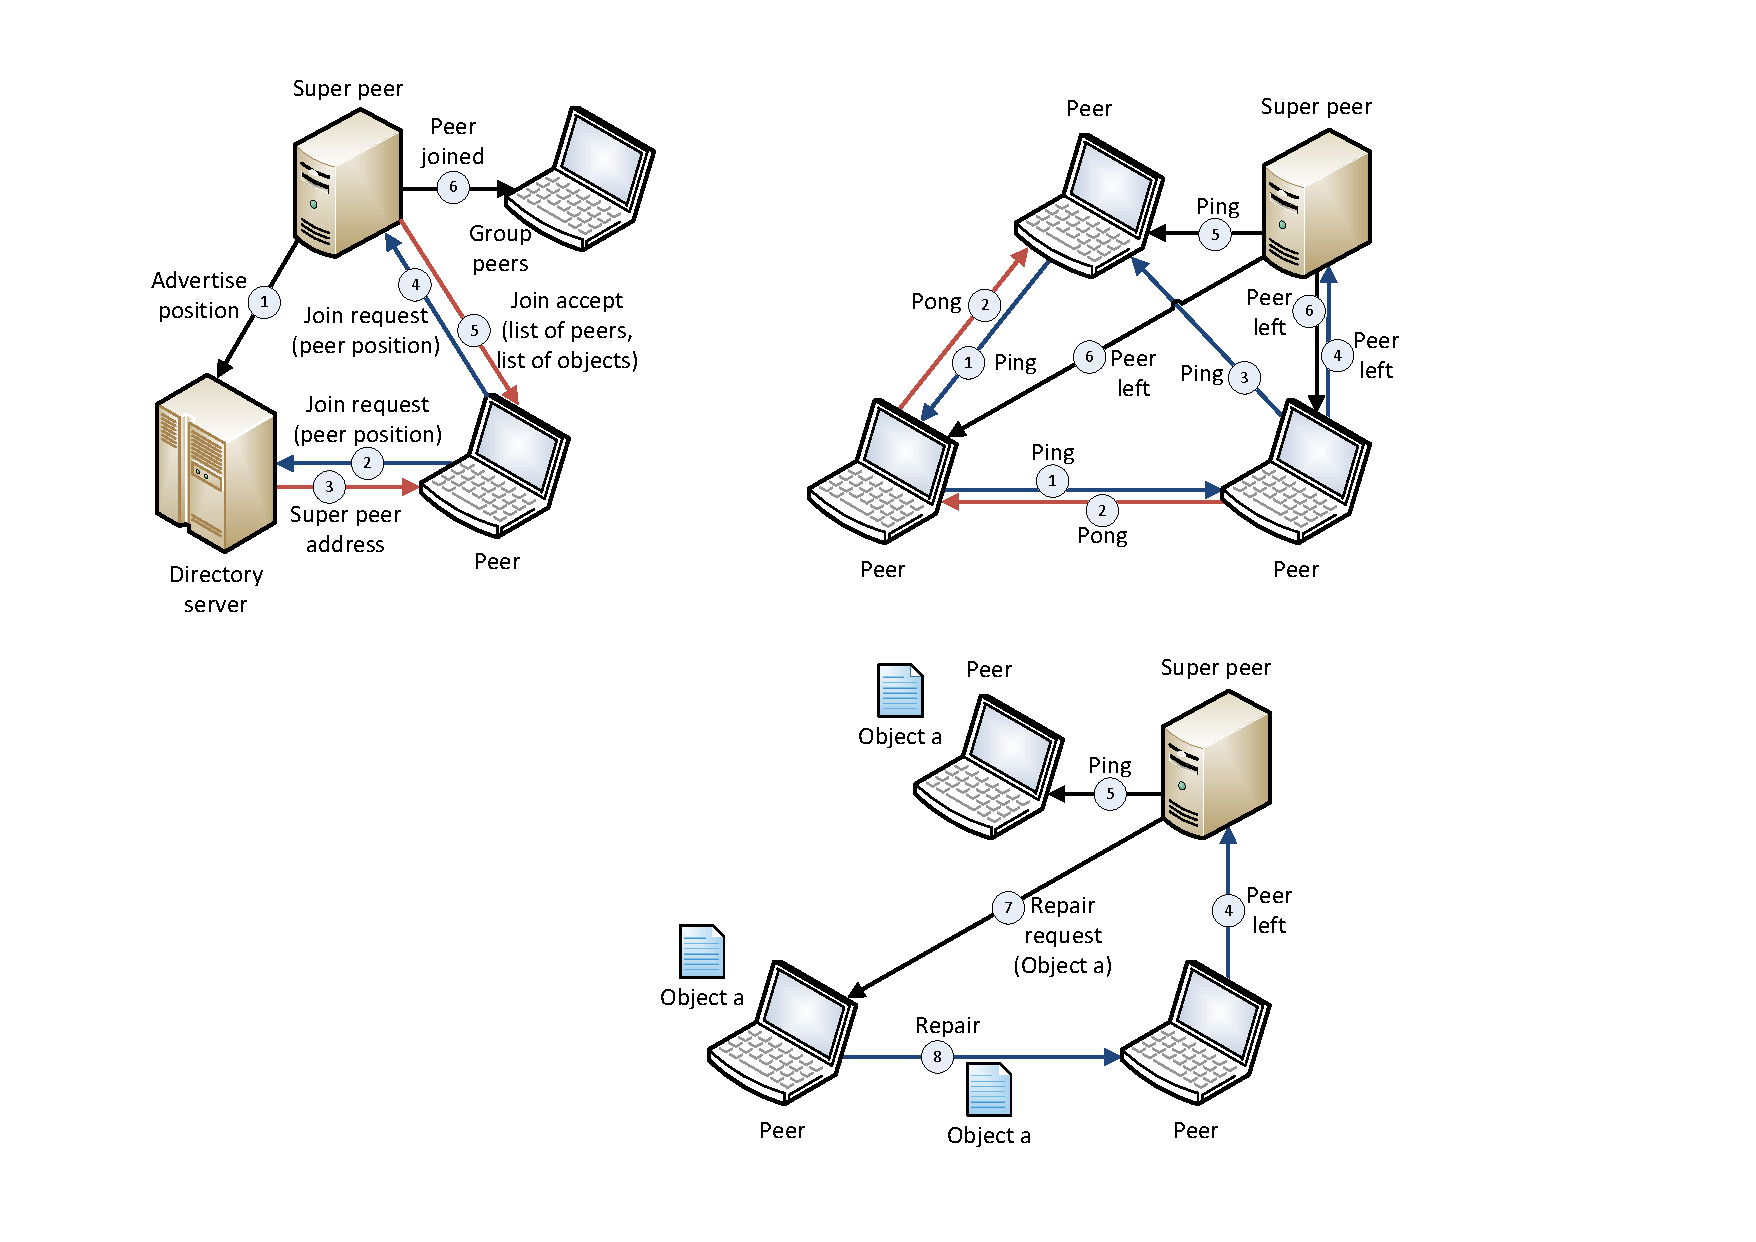
\includegraphics[clip=true, viewport=110mm 15mm 225mm 100mm, width=0.7\columnwidth]{Pithos_mechanisms}
 \caption{Pithos repair mechanism}
 \label{fig_pithos_repair}
\end{figure}
%
\begin{enumerate}
\setcounter{enumi}{6}
\item After a the super peer has detected that a peer has left and has informed all other peers, the super peer selects a peer that contains an object that was destroyed by the leaving peer and requests that that object be replicated.

\item The peer receiving the replication request from the super peer selects another peer in the group that does not already contain the object and replicates the object on the selected peer.
\end{enumerate}

Leaving repair attempts to minimise the super peer load by only repairing objects when a node leaves the network. This is as opposed to periodic repair, where the super peer has to constantly cycle though its list of object replicas and verify the number of replicas currently stored in the system.

\section{Satisfying the use cases}
All Pithos modules and mechanisms that ensure adherence to the storage requirements have now been described. What remains to be described is how the use cases presented in Section \ref{use_cases_goals} are designed on the architecture that adheres to the storage requirements.

It is assumed that some higher layer exists above Pithos, which generates requests. According to our generic consistency model, these requests will arrive from the game logic or object updater. It should be noted that a request can be a storage, retrieval, modification or removal request and does not only imply a request for data, i.e. a retrieval request.

\subsection{Store}
\label{pithos_store}

\begin{figure}[htbp]
 \centering
 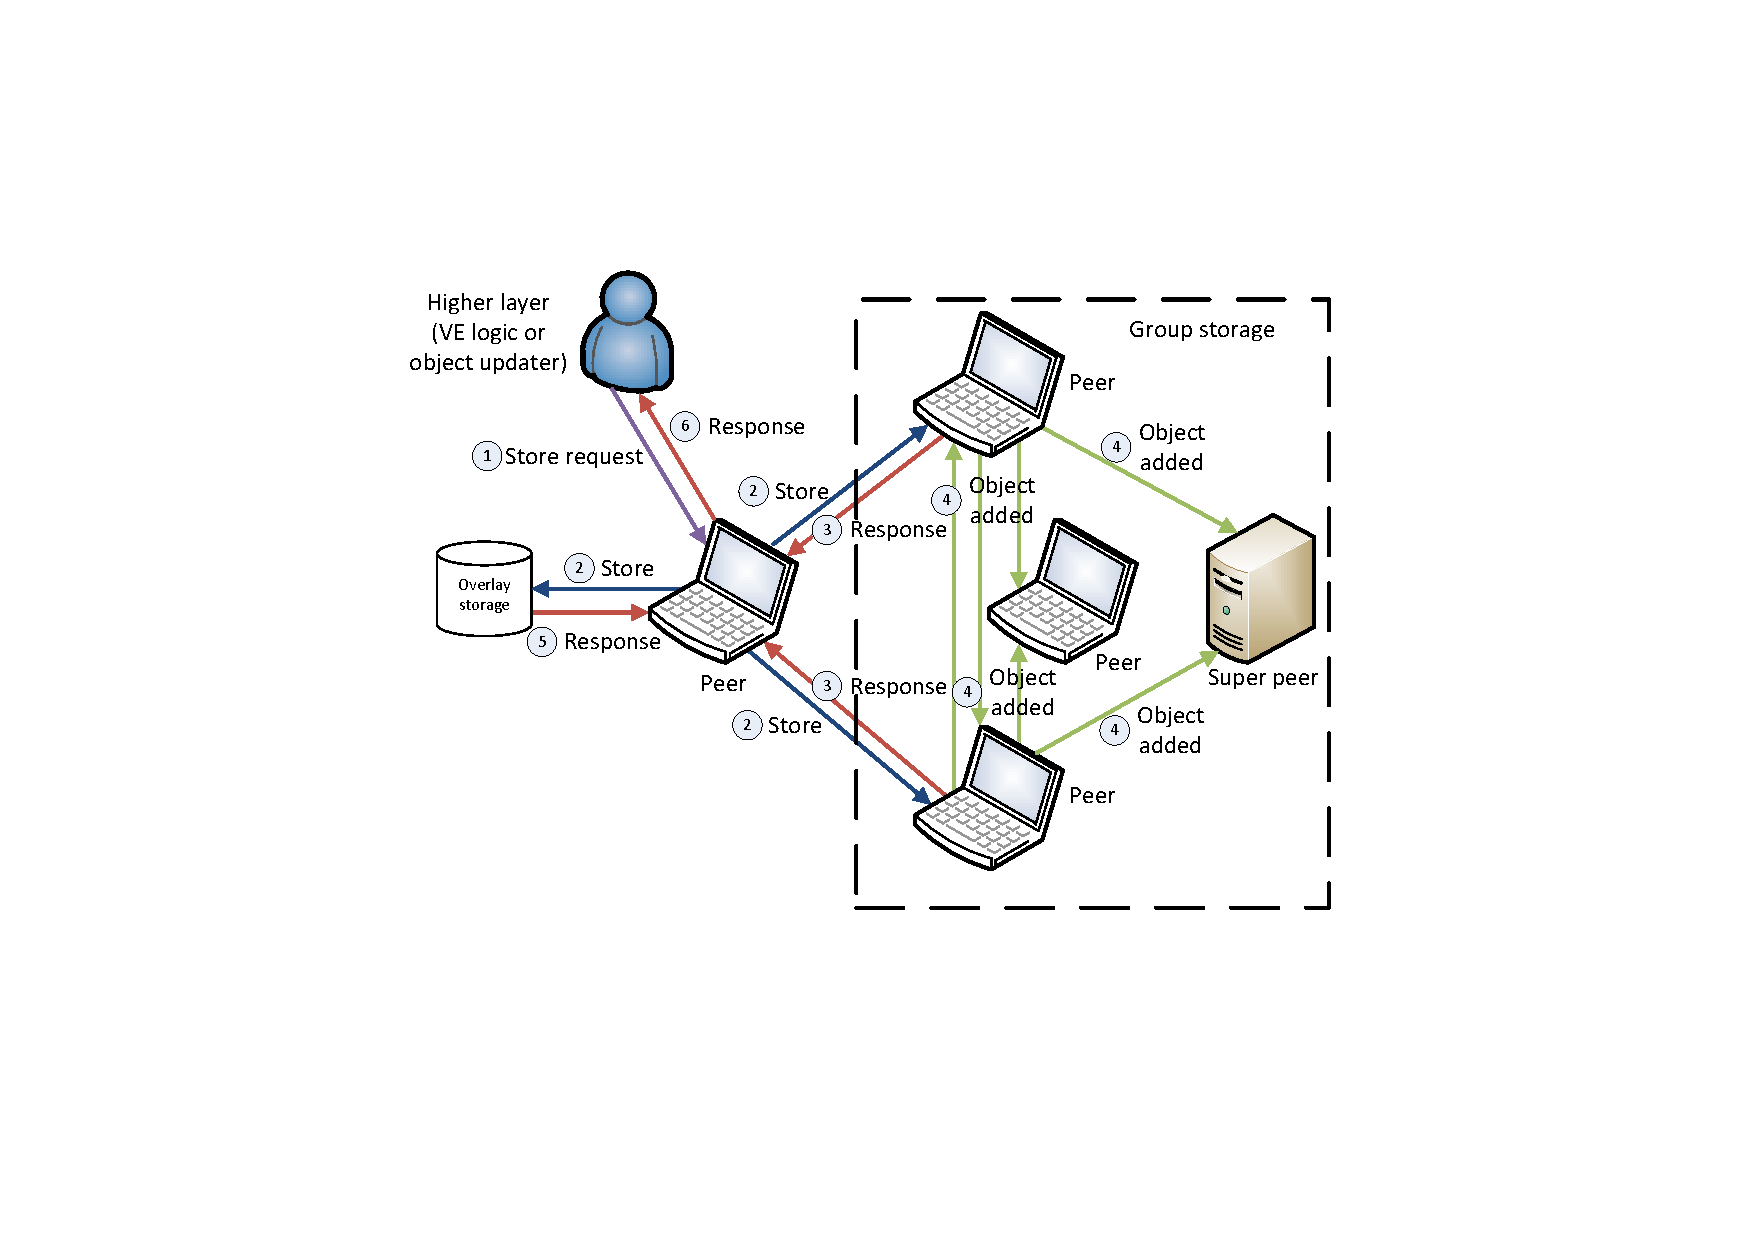
\includegraphics[clip=true, viewport=67mm 55mm 228mm 165mm, width=0.7\columnwidth]{Pithos_use_case_store}
 \caption{Pithos storage}
 \label{fig_pithos_storage}
\end{figure}
%
Referring to Figure \ref{fig_pithos_storage}, Pithos storage works as follows:
%
\begin{enumerate}
\item The higher layer is expected to send a storage request to Pithos, containing the object to be stored.

\item Pithos contains logic that relays the storage request to both peers in group storage as well as overlay storage.

\item The group storage module will store the object in its local authoritative object store and acknowledge the reception of the object by sending a response message to the source node.

\item Each peer successfully storing a received object will inform all group peers, as well as the super peer, of the new object stored. The peers and super peer can add this information to their group ledger, used to serve retrieval requests.

\item Sometime after group storage has completed, overlay storage will also complete. Overlay storage informs Pithos logic of the success or failure of the request.

\item Pithos monitors all responses and records the success or failure of each request. When a sufficient number of responses have been recorded, Pithos informs the higher layer of either a successful or failed store.
\end{enumerate}

Overlay storage implements an existing DHT and it is assumed that overlay storage correctly handles the storage request.

The number of nodes selected from the group ledger relates to the number of required object replicas. Nodes are selected in a uniformly random fashion, making sure to never select the same node more than once. If a node is selected more than once, it reduced the effective number of replicas in the network, which reduces the expected object lifetime. A detailed discussion of object lifetime is presented in Chapter \ref{chp:MODELLING}.

The question arises as to what constitutes a sufficient number of responses. Two types of storage mechanisms have been implemented in Pithos: ``safe'' and ``fast''. With safe storage, Pithos waits for all responses to be received. Only after all responses are received is a decision made whether the store was successful or not. If more than half of the group stores as well as the overlay store was successful is it considered a successful store. The higher layer is informed of the status of the store request at this time. Fast storage has Pithos wait for the first successful response, before informing the higher layer of success. If all responses are failures, it informs the higher layer of a failure.

Because safe storage ensures that most of the replications are successfully stored, there is a smaller chance of it reporting a false positive than for fast storage. The disadvantage is that from the point of view of the higher layer, and by extension any system that uses Pithos, safe put requests have a lower responsiveness. Fast storage on the other hand is no less reliable than safe storage, but the chances of a false positive being reported to the higher layer is greater. The advantage of fast storage is that the from the perspective of the module using Pithos, it is performed faster than safe storage. The higher layer can, therefore, start using the stored object faster. A comparison of fast and safe storage is performed in Chapter \ref{chp:EVALUATION}.

\subsection{Retrieve}
\label{pithos_retrieve}

%Talk about the types of keys (content key and name key) and how objects will be named in the storage system.

\begin{figure}[htbp]
 \centering
 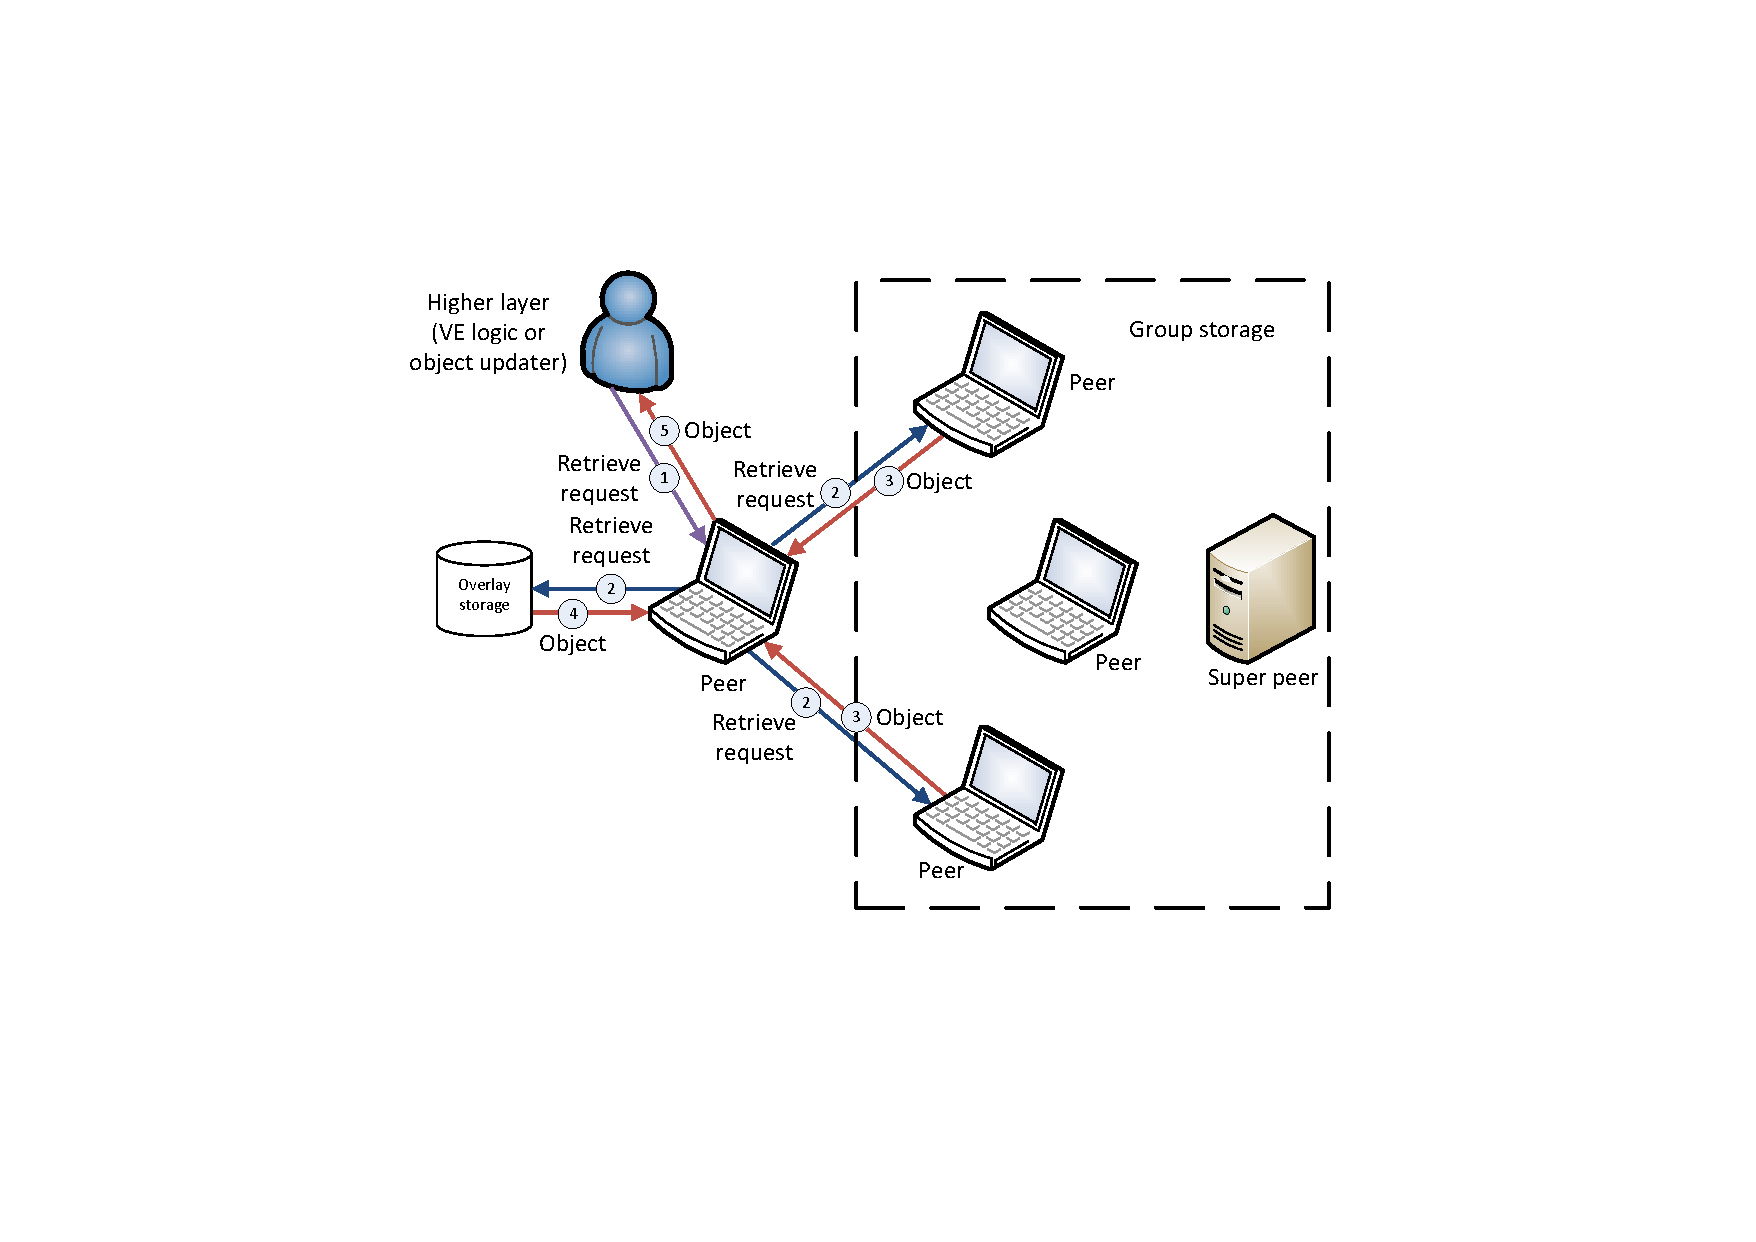
\includegraphics[clip=true, viewport=67mm 55mm 228mm 165mm, width=0.7\columnwidth]{Pithos_use_case_retrieve}
 \caption{Pithos retrieval}
 \label{fig_pithos_retrieval}
\end{figure}
%
The process of retrieving data is very similar to that of storing it. With reference to Figure \ref{fig_pithos_retrieval}, retrieval works as follows:
%
\begin{enumerate}
\item The retrieve request, received from the higher layer, contains the hash of the object name which the higher layer requires.

\item Pithos first checks whether the object that was requested exists within the group by checking its group ledger. This is required, because the higher layer might have requested an object that is stored in another group. Out-of-group requests are only serviced by overlay storage. If the object is housed in the Pithos peer's local store, the object is sent to the higher layer. If the object is not housed locally, Pithos requests the object from both overlay and group storage.

    The group ledger is used to determine which group peers contain which objects. The number of peers selected depends on the retrieval type. Three retrieval types exist: fast, parallel and safe retrieval. Fast retrieval selects a single peer for object retrieval. Parallel and safe retrieval select multiple peers to concurrently retrieve an object from. More requests sent in parallel improves the probability of the request succeeding as well as reduce the time it takes to serve the request.

\item When the retrieval request is received at the destination peer, the object is retrieved from local storage, attached to a response message and sent to the requesting peer.

\item Sometime after group retrieval has completed, overlay retrieval will also complete and send the object, stored in the overlay, to Pithos.

\item After Pithos has received a sufficient number of responses, it informs the higher layer of either a successful or failed retrieval. The object itself is attached to a successful request response.
\end{enumerate}

Retrieve requests mainly fail because of nodes leaving a group. If a node leaves before it can serve an object, the object request fails. If multiple requests are sent with parallel retrieval, it improves the chances of contacting a node that is not about to leave, which improves the probability of retrieval success. More requests also improve lookup times, since some peers might be geographically closer to the requesting peer, thereby possessing a lower latency.

Sending multiple requests improves the chances of contacting a peer that is closer, which improves the responsiveness of the systems. Fast and parallel retrieval sends the first successful  response, and therefore, the first successful object, to the higher layer. It replies with failure if all requests failed.

The safe retrieval request is more resistent to malicious nodes. For safe retrieval, Pithos waits for a specified number of responses. It then compares all objects received from successful responses and sends an object to the higher layer that had the most matches when compared. This is to counter a malicious peer that might have altered some of the objects before sending them. Safe retrieval implements the quorum mechanism, described in Section \ref{quorum}.

As shown in Figure \ref{fig_pithos_retrieval}, the super peer is not used for retrieval requests. This is not necessary, since all peers contain lists of all objects. The super peer should, however, still contain it own group ledger, to inform peers joining the group of the peers and objects already in the group. Not requiring the super peer to manage object requests prevents the super peer from becoming overloaded.

\subsection{Modify}

Modifying data is similar to storing data. A request to modify a specific object is received from the higher layer. The request specifies the object ID, the parameter that has to be modified and the new value of the parameter. The update is delivered to Pithos, which forwards the request to both group and overlay storage. The Oversim DHT handles the modify request and responds with success or failure. Group storage received the modify request and checks the group ledger whether the object exists within the group. If the object does not exist in the group, it is only modified in the overlay. To keep track of modified objects, each object has a version number that is incremented every time an object is modified. This allows retrieve requests to select the object with the latest version number to be sent to the higher layer.

If the object exists within the group, all peers that contain the object are identified from the group ledger and modify requests are sent to them. The modify request is sent to the destination peer, where the object in the local store is updated and its version number incremented. If a retrieve request receives objects with multiple version numbers, it selects the set of objects with the latest version number for ``fast'' or ``safe'' comparison.

\subsection{Remove}

Removal is handled by the object TTL. It is not possible to define an explicit remove operation for overlay storage, since a peer may be off-line when the removal request is sent. If the peer rejoins the network, the object becomes available again. Object TTL ensures that the storage space requirements does not increase indefinitely during the lifetime of the storage system.

\section{Conclusion}

This section describes the Pithos conceptual design. The use cases are defined from the perspective of the higher layer that wishes to make use of Pithos's services. The conceptual design is first described in terms of how it ensures the storage requirements are met. The design the use cases are then described in terms of the designed architecture.

\chapter{Pithos Implementation}
\label{chp:IMPLEMENTATION}

The previous chapter discussed the conceptual design of Pithos. Pithos has been implemented in Oversim \cite{OverSim_2007}, a P2P simulation environment based in Omnet++, which allows for the measurement of identified requirements. Furthermore, it allows for the comparison of the current model with other state persistency models.

\section{Oversim}

Oversim is a peer-to-peer and overlay simulation framework for the Omnet++ simulator. Oversim allows for the simulation of many well known structured or unstructured overlay protocols. It also allows for the development of applications that can use the already implemented overlays in a well defined architecture.

\subsection{Motivation}

To allow for greater control of the environment, as well as greater scale, it was decided to implement the first version of Pithos as a large scale network simulation. A simulation allows for careful selection of the environment parameters and tight control of the parameter values. This in turns allows one to keep all but one parameters constant and evaluate the effect of a design decision on the system for varying values of the free parameter.

The underlying Omnet++ simulation environment is a powerful network simulator in its own right. It allows for robust message and module definitions and contains many tools to assist with simulation measurement and monitoring, for example global statistics gathering tools and built-in plotting tools.

Simulation also allows for greater scalability and simulating on a network with global Internet characteristics. Greater scalability is achieved, because thousands of nodes can easily be created, where all the nodes have global scale latency characteristics.

Implementing a large scale network application in the real-world would require thousands of computers spread across the globe. Such an environment will contain many variables out of the designer's control. Issues such as router congestion for example varies from day to day, which will produce varying latency results.

Because of these reasons, it was decided to first implement Pithos in simulation. This allows for the perfection of the design, under laboratory conditions, before the real world implementation is completed.

Pithos is intended for future real world implementation, however, so all modules created were written in such a manner to allow for easy porting. No tasks that are performed in Pithos make use of any simulation ``short cuts'', such as accessing the global peer list. Only statistics gathering modules are allowed to make use of these simulation features.

\subsection{Underlay network}
\label{oversim_underlay}

At the base of an Oversim simulation is the underlay network. The underlay network determines the types of nodes in the Oversim simulation. Three underlay types exist: the ``simple'', ``INET'' and ``SingleHost'' underlays \cite{oversim_applications}.

In the simple underlay, node latencies are determined by the distance between nodes placed in a two dimensional Euclidean space. The positions of the nodes are chosen to match the latencies of the CAIDA/Skitter Internet mapping project \cite{caida_skitter}. Different nodes are also assigned different bandwidth and jitter parameters to simulate a heterogenous network. The simple underlay, therefore, captures the delay characteristics of a global scale network in an abstract way. The simple underlay network is ideal for simulating large scale overlay networks because of its simplicity and high accuracy \cite{oversim_applications}.

The INET underlay is based on the Omnet++ INET underlay and allows for the simulation of the complete IP level stack. This includes backbone routers and gateways. It also contains many implemented MAC layer protocols. The INET underlay is well suited to simulating lower level communication protocols or wireless protocols such as IEEE 802.11 (Wi-Fi).

The SingleHost underlay allows for interaction with a physical network. It allows for the implementation of physical nodes, running on networks computers. These physical nodes can then connect to a simulated network and receive packets with bandwidth and delay characteristics as if they were situated on a network with the simulation's specific characteristics.

To be able to simulate Pithos for the large numbers of nodes required, as discussed in Section \ref{scalability_req}, it runs on the simple underlay. Pithos is dependant on the delay characteristics of the lower level protocols, but the CAIDA and Skitter measurements capture these quantities in their measurements. The reasons why the underlying network shows certain delay characteristics are not important. A focus is also not currently placed on the effects of transient background traffic flows in the Internet architecture on which Pithos executes.

\begin{figure}[htbp]
 \centering
 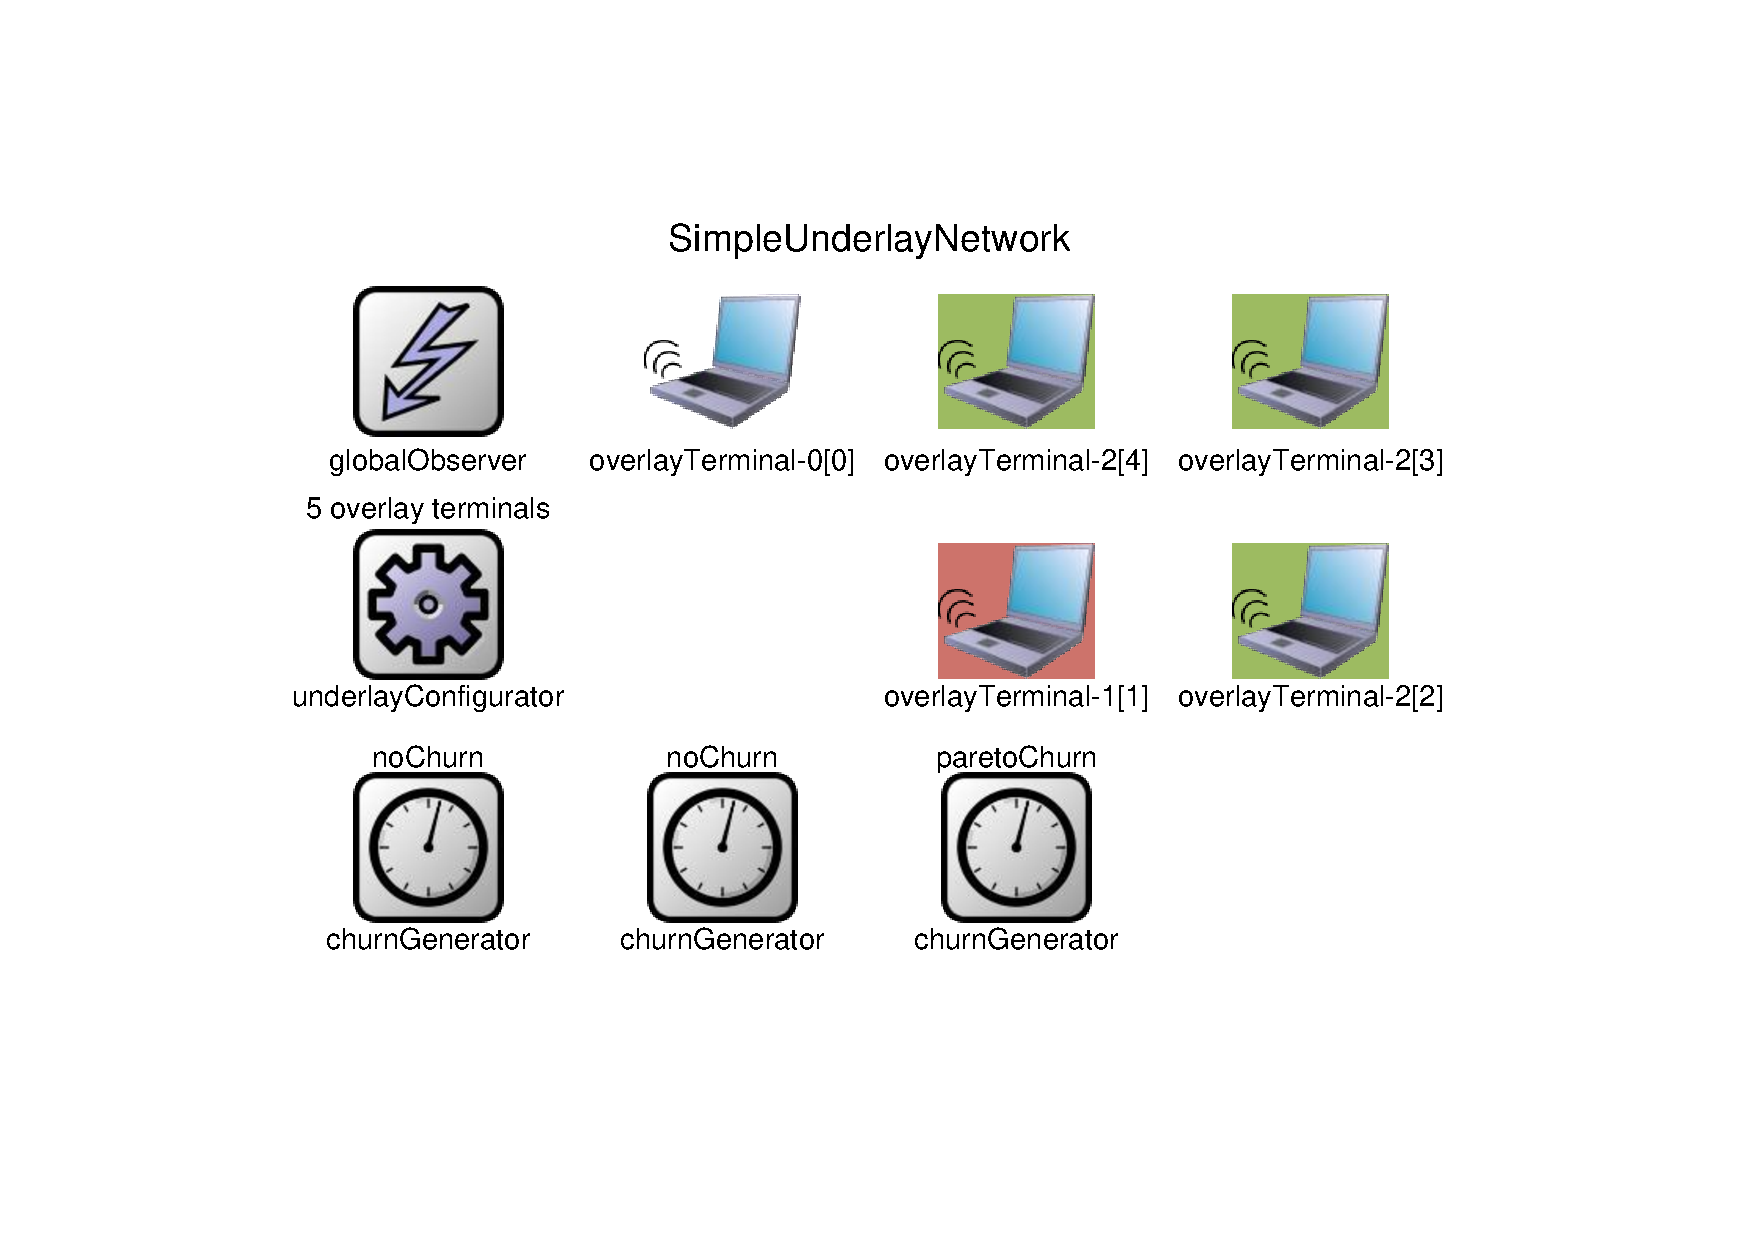
\includegraphics[clip=true, viewport=49mm 48mm 245mm 173mm, width=0.5\columnwidth]{Oversim_terminals}
 \caption{The Oversim simple underlay network with the three Pithos terminal types}
 \label{fig_oversim_terminals}
\end{figure}

Figure \ref{fig_oversim_terminals} shows the Pithos simple underlay network after the first five nodes have been generated. Each overlay terminal is an Oversim node containing its own protocol stack. The underlay configurator is responsible for setting up the network. The global observer contains the global node list, global statistics and parameters modules. It is used to generate global statistics and by the lower levels to keep track of all nodes.

Three churn generators also exist, one for generating each of the three Pithos node types. Churn generators model users joining and leaving the network. There are three types of churn generators: ``no churn'', ``lifetime churn'' and ``Pareto churn''. The ``no churn'' churn generator creates nodes every specified number of seconds until a specified number of nodes are reached and does nothing further. This generator can be used to test simple networks, where churn is not an issue, or for initial testing of the first prototype.

Lifetime churn creates nodes with specified average lifetimes, sampled from an exponential distribution. This is a distribution regularly used to model lifetimes in reliability engineering. Pareto churn samples node lifetimes from a Pareto distribution (type of heavy-tailed distribution), instead of an exponential distribution. Pareto churn requires mean node lifetime as well as mean node dead time to be specified.

A node type is determined by the protocols executing on every layer of the Oversim architecture. As discussed in Section \ref{key_modules_mechs}, the Pithos node types are the peer, super peer and directory server.

\subsection{Node architecture}

\begin{figure}[htbp]
 \centering
 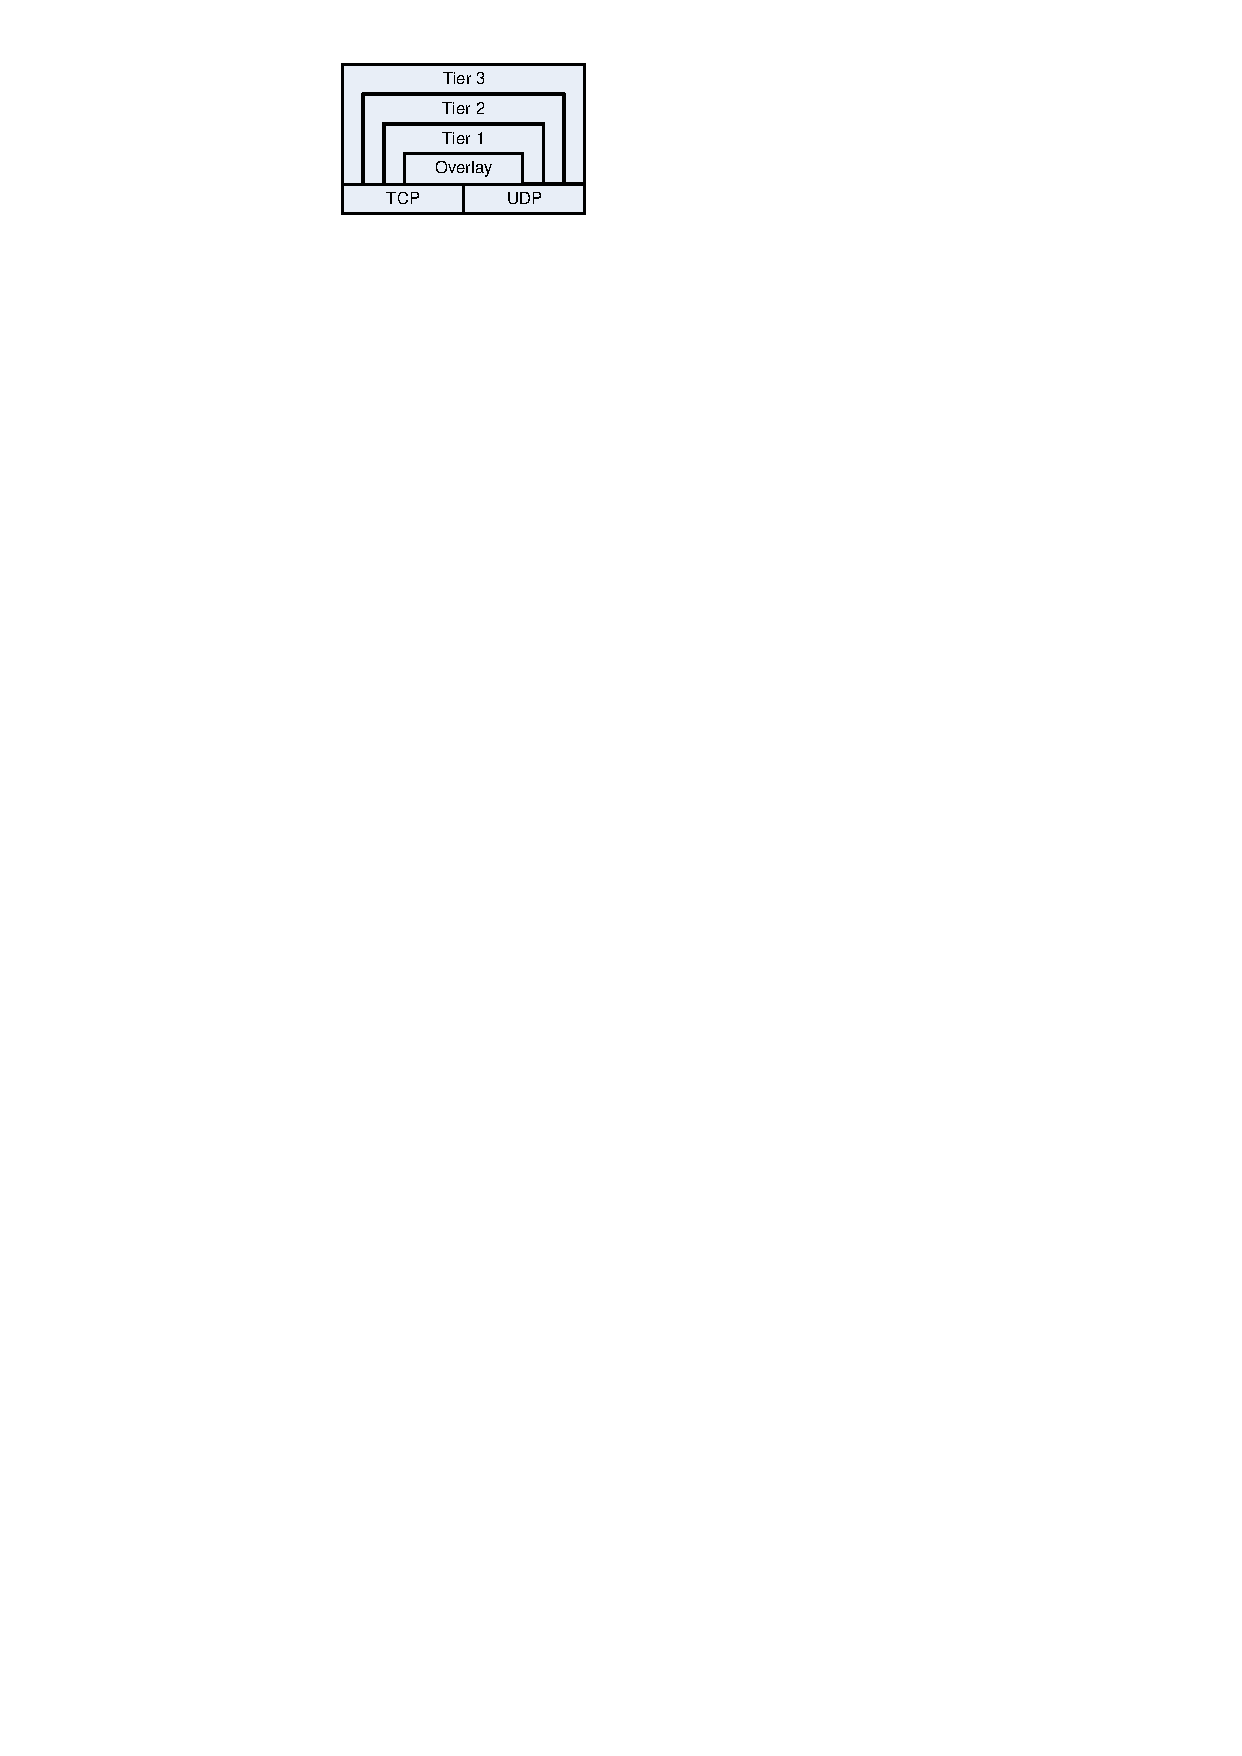
\includegraphics[clip=true, viewport=57mm 260mm 100mm 287mm, width=0.5\columnwidth]{Oversim_layers}
 \caption{Oversim node architecture layers}
 \label{fig_oversim_layers}
\end{figure}

%Also show the Oversim picture

Every node in Oversim contains a layered architecture, as shown in Figure \ref{fig_oversim_layers}. The Oversim node architecture contains the layers: TCP, UDP, Overlay, Tier 1, Tier 2 and Tier 3.

The transport control protocol (TCP) and user datagram protocol (UDP) are both transport level protocols, according to the OSI protocol stack specification. These two layers are the lowest communications layers in Oversim and allows message passing to other nodes.

The overlay layer is where the P2P overlay is housed. This can be any of the well known structured or unstructured overlays, such as Pastry, Chord or Gia. The three tiers above the overlay layer are the application level layers and is where application that use an overlay may be implemented. Three application layers are allowed.

Tier 1 can communicate with the Tier 2, overlay, TCP and UDP layers. Tier 2 can communicate with the Tier 1, Tier 3, TCP and UDP layers. Tier 3 can communicate with the Tier 2, TCP and UDP layers. Internal communications are usually between tiers and TCP and UDP communication occurs when a layer wishes to send a message to the same layer on a different node.

\begin{figure}[htbp]
 \centering
 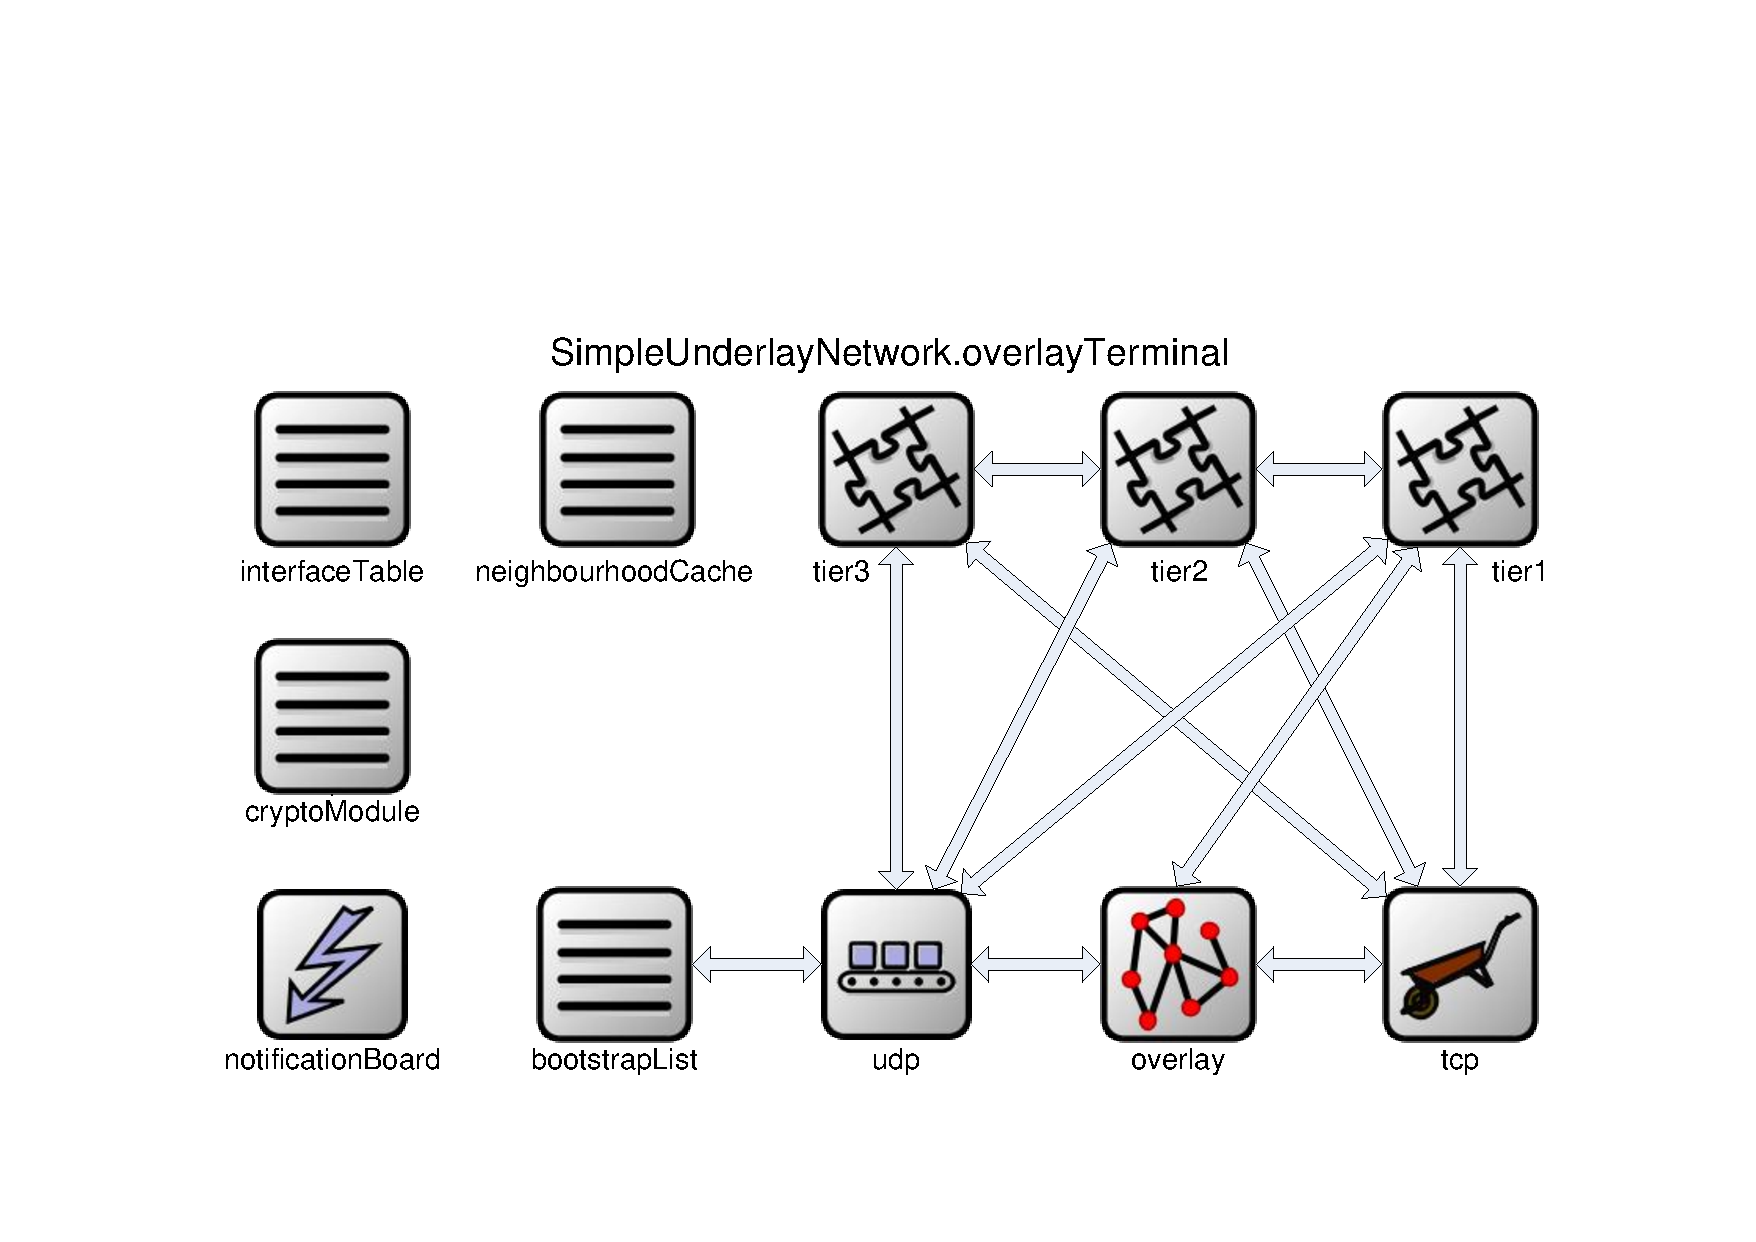
\includegraphics[clip=true, viewport=33mm 27mm 262mm 197mm, width=\columnwidth]{Oversim_architecture}
 \caption{The components of an Oversim terminal, including the tiered node architecture.}
 \label{fig_oversim_architecture}
\end{figure}
%
Figure \ref{fig_oversim_architecture} shows the complete Oversim node architecture. The tiers, udp, tcp and overlay are connected as explained earlier. UDP is also connected to a bootstrap list module, which assists nodes with joining the UDP network. The neighbourhood cache, interface table, crypto module and notification board modules are also present, but these modules are unused in Pithos.

    \subsection{Generic consistency extension}
    \label{generic_consistency_extension}

%Show the generic consistency architecture in Oversim

To allow Oversim to simulate a complete consistency architecture, we extended the Oversim framework itself. The three tiers were replaced with all the elements identified in the generic consistency model in Section \ref{generic_event_update_model}. Practically, this required the implementation of a new type of overlay terminal type, replacing the tiers with the following layers:
\begin{itemize}
\item agent,
\item event layer IM,
\item event dissemination,
\item event ordering,
\item game logic,
\item authoritative object updater,
\item authoritative object store,
\item update layer IM,
\item update dissemination,
\item object merger,
\item non-authoritative object updater,
\item non-authoritative object store,
\item display updater,
\item overlay Storage.
\end{itemize}

Every new layer can communicate with the layer above and below it, and can also communicate with its counterpart on another node using UDP or TCP. This allows for the consistency model to be distributed amongst any number of nodes. A module can either send its information to the layer below it within the same node, or it can send it to the layer below it on another node.

Every module can contain a collection of sub-modules which implements the layer itself. It the layer is not implemented, a dummy layer may be specified. The Pithos implementation is located within the authoritative object store module. An application that provides Pithos with test inputs called ``PithosTestApp'' is situated within the authoritative object updater layer. Pithos also makes use of overlay storage, which is implemented in the overlay storage module. Overlay storage requires a P2P overlay for routing purposes, which is why it is connected to the overlay layer.

\section{Module types}
\label{pithos_module_types}

\begin{figure}[htbp]
 \centering
 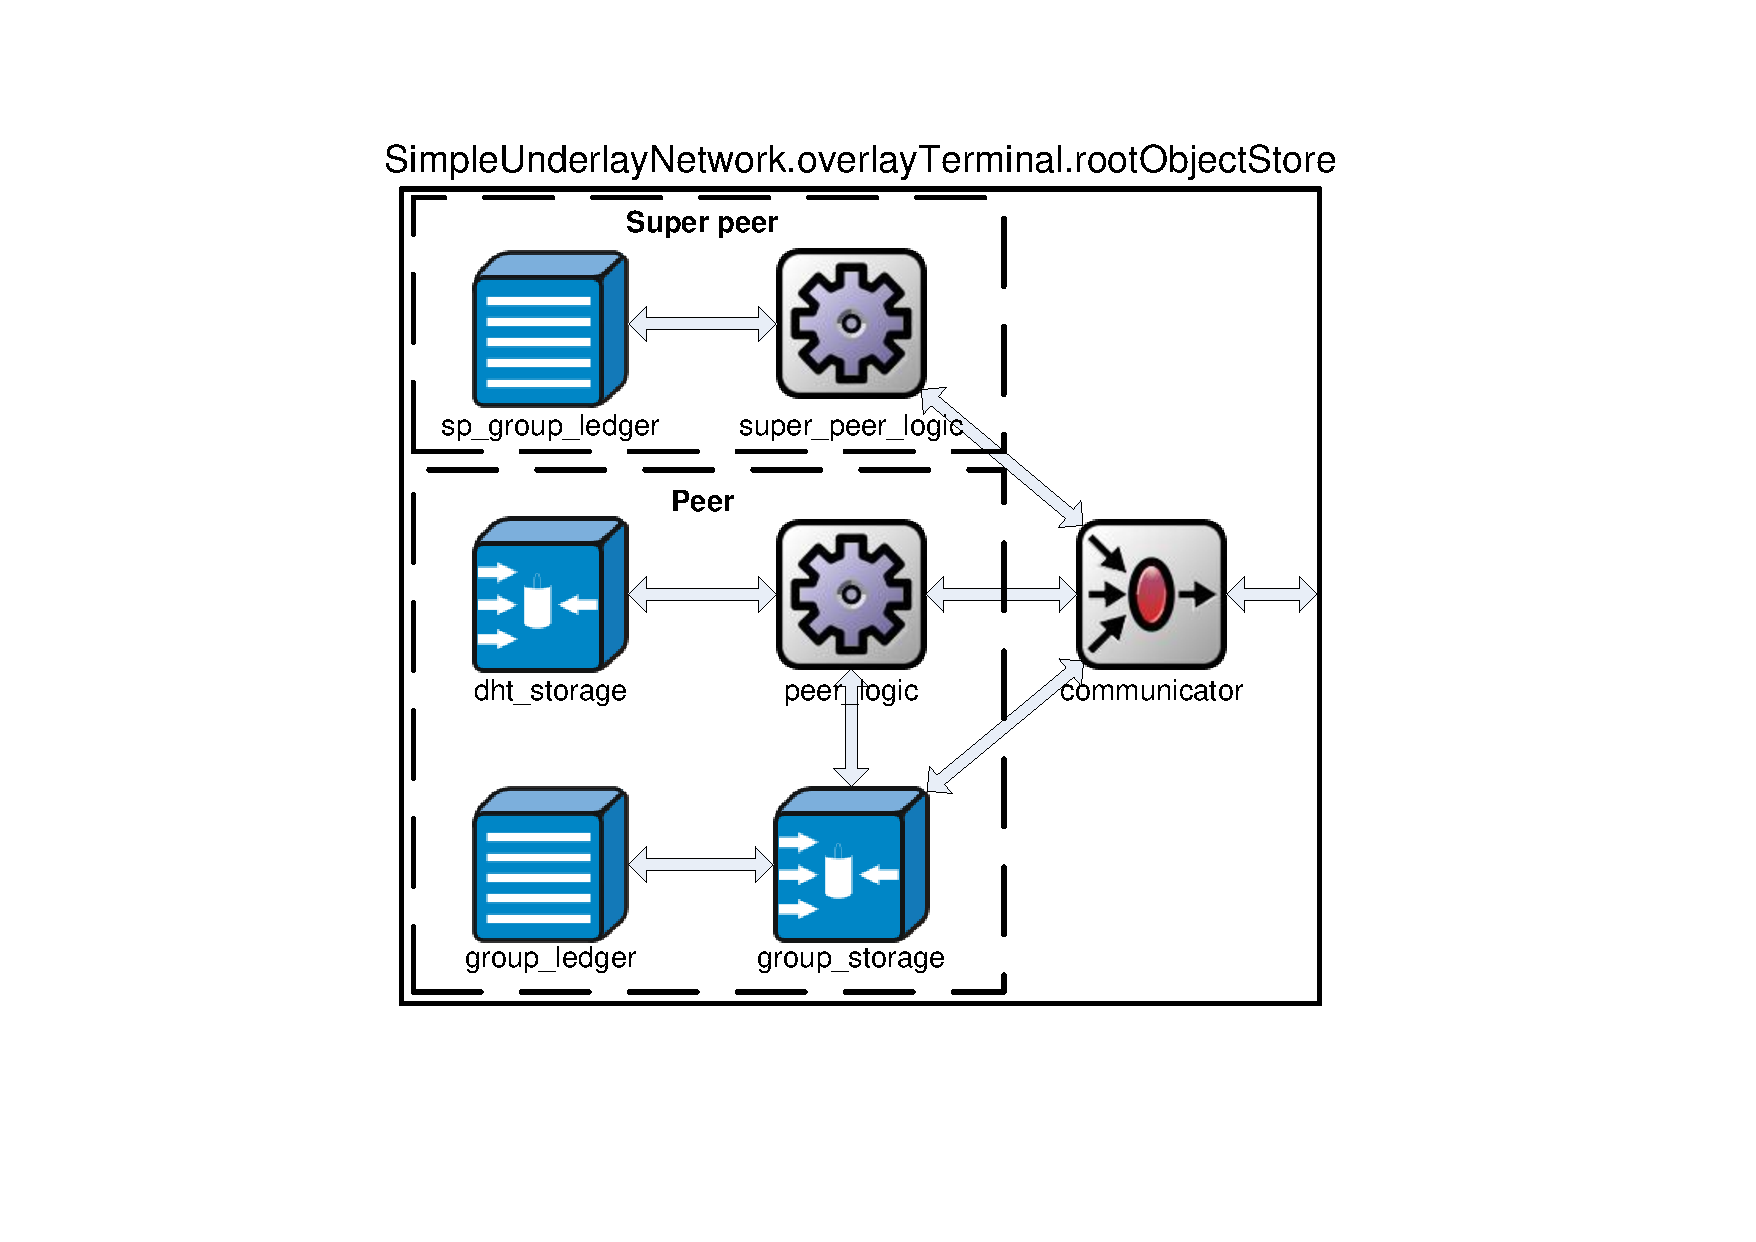
\includegraphics[clip=true, viewport=64mm 39mm 227mm 186mm, width=0.5\columnwidth]{Oversim_root_object_store}
 \caption{Pithos super peer and peer modules in Oversim}
 \label{fig_oversim_root_object_store}
\end{figure}
%
Figure \ref{fig_oversim_root_object_store} shows the Pithos modules related to the super peer and peer module types. The figure is divided into three sections: Super peer, peer and communicator.

\subsection{Communicator}

A simple module in Omnet++ is a module that implements a C++ class. All modules in Figure \ref{fig_oversim_root_object_store} are simple modules. Compound modules also exist that are combinations of simple modules, where the simple modules are connected to each other and external gates in some way.

Oversim requires a single simple module to be of type: ``BaseApp''. Oversim delivers messages from the layers above and below a layer to the module extending the BaseApp module. This means that because of Oversim's architecture, all messages must traverse a single module. When Pithos was designed, it was decided that placing all functionality in a single module would be a bad design decision, going against the philosophy of modular design. A single module would not allow for a modular implementation and would make future extensions more difficult.

The communicator module receives and sends all communications to the upper and lower layers on behalf of the other Pithos modules. All messages received or sent are, therefore, routed through the communicator module. The design philosophy of the communicator module was to make it as transparent as possible. Another function of the communicator module was outbound message verification. The communicator module ensures that all sent messages contain a destination IP address, source IP address and packet type information.

Transparency was achieved by designating certain gates for certain types of traffic. If a message is received on a gate with a specific purpose, that message is processed in a way consistent with that purpose and then transmitted. This design allows other modules to be expanded with new message types. Those message then only have to be sent to the correct gate to ensure correct handling of the message. The addition of a new message type, therefore, rarely required alterations to the communicator module.

\subsection{Super peer logic}
\label{pithos_module_types_sp_logic}

The super peer logic module implements all the functionality of the super peer node, except for keeping track of group objects. The tasks of the super peer logic include handling joining peers, facilitating peer migration, ensuring group consistency (Section \ref{group_consistency_implementation}), initiating object repair (Section \ref{object_repair_implementation}) and maintaining a list of group objects and a list of peers on which those objects are stored (Section \ref{pithos_module_types_ledgers}).

\subsection{Peer logic}

Peer logic
\begin{enumerate}
  \item  receives all store, retrieve and modify requests from the higher application layer,
  \item forwards those requests to the required modules,
  \item forwards responses received from modules to the higher layer,
  \item keeps track of all outstanding requests (Section \ref{pending_rpcs_implementation}), and
  \item implements the quorum mechanism.
\end{enumerate}

\subsection{DHT storage}

The DHT storage module forms part of the peer node. The DHT storage module interfaces with the overlay storage module on behalf of the peer. The DHT storage module received requests from the peer logic modules for overlay storage services. The DHT storage module also keeps track of all outstanding overlay storage requests.

In the Oversim simulation, the DHT storage module interfaces with Oversim's DHT implementation, written by Gregoire Menuel and Ingmar Baumgart. The DHT implementation itself is located in the overlay storage module of the extended Oversim node architecture that represents the generic consistency model, as described in Section \ref{generic_consistency_extension}.

The Oversim DHT implementation contains data structures to store data, route requests via the overlay to other DHT modules and allows peers to join a network-wide overlay. It supports store, retrieve and modify requests. The Oversim DHT implementation meets all Pithos's overlay storage requirements and is able to run on any of the overlay implemented in Pithos.

\subsection{Group storage}

The group storage module forms part of the peer node. It receives requests from the peer logic module for group storage services. The group storage module
\begin{enumerate}
  \item handles group store, retrieve and modify requests from the peer logic,
  \item maintains a view of all peers currently in the group,
  \item maintains an object store where it stores some subset of the group objects,
  \item is responsible for the administration of group membership on behalf of the peer,
  \item monitors the availability of group peers and informs the the super peer of peers that left the group,
  \item informs the group of new object stored, and
  \item repairs objects if requested to do so by the super peer.
\end{enumerate}

\subsection{Ledgers}
\label{pithos_module_types_ledgers}

The group ledger is an abstract data type that maintains lists of all objects stored in the group, as well as all peers that are part of the group. The group ledger is used by the group logic and super peer logic modules to keep track of all group objects and peers.

The group ledger was designed for efficient storage, while still allowing high speed access to data. In order for the ledger to be efficient, it implements a map of object ledgers, where each object ledger contains object information and a list of peers where that object is stored on. The group ledger also contains a peer ledger list, where each peer ledger contains a list of objects that are housed on that peer.

In the object ledger, each entry in the peer list is a reference to peer information contained in the peer ledger. In the peer ledger, each entry in the object list is a reference to peer information contained in the object ledger. This means that peer and object information are only stored once, and always referred to by references. This dually linked structure allows for searching in any direction. Objects are stored in a map, since there might be thousands of objects in a group, compared to tens of peers. Efficient object lookup is, therefore, a priority, whereas sequential peer search is sufficient.

The ledger abstract data type is implemented using reference counting pointers (smart pointers), to avoid any memory leaks that might have occured due to incorrect memory management of the large number of pointers present.

\section{Implementation issues relating to key mechanisms}
\label{key_mechanisms}

%%%%%%%%%%%%%%%%%%%%%%%%%%%%%%%%%%%%%%%%%%%%%%%%%%%%%%%%%%%%%%%%%%%%%%%%%%
% For every mechanisms, reference where the results of that mechanism will
% be shown.
%%%%%%%%%%%%%%%%%%%%%%%%%%%%%%%%%%%%%%%%%%%%%%%%%%%%%%%%%%%%%%%%%%%%%%%%%%

While the previous chapter describes all key mechanisms, some adjustments had to be made to allow for correct functionality under Oversim. The key mechanisms that have simulation specific implementations are also discussed in this section.

\subsection{Joining the network and grouping}

As described in Section \ref{join_mechanism}, in order to join the network, a super peer should supply its location in the virtual environment (VE) to the directory server. A joining peer should also supply its location to the directory server, so the directory server may supply the joining peer with a super peer's address to join.

Because Pithos is not functioning in an actual VE, peers have no locations. For simulation purposes, each super peer is assigned a random location created by sampling both an x and a y coordinate from a uniform random distribution in a fixed range (0 to 100). Joining peers are assigned positions in the same uniform random manner when they are initialised.

These positions are used by the super peers and peers when contacting the directory server. The directory server supplies the peer with the address of the closest super peer to join. This is an implementation of a simple centralised grouping algorithm. Super peers effectively control certain areas in the VE, based on their and their neighbours' locations.

Although the distributed grouping techniques discussed in Section \ref{grouping_design} are exchanged for a simple centralised scheme, it serves its purpose to group all peers into groups controlled by super peers for the simulation. In a practical implementation, this solution is still applicable, but the directory server might become overloaded. If this happens, a more powerful directory server can be used, or one of the distributed grouping algorithms may be implemented.

\subsection{Group migration}
\label{group_migration_implementation}

To simulate the effect that user movement will have on objects stored in Pithos, PithosTestApp is designed to generate position updates.

PithosTestApp simulates a user moving around in a virtual world. This is done by having PithosTestApp generate a new random position chosen in the same way as when a node joined a group: by selected x and y coordinates in a uniformly random fashion. A position update timer determines when a node's position should change.

It is accepted that the movement this scheme will generate will not match the way users move in a virtual world. Modelling accurate user movement is, however, not important for the Pithos simulation. Storing and retrieving objects in Pithos only depends on which group a user occupies and how Pithos handles a user that moves to another group. The order in which a user might enter groups or, in fact, the specific group that a user moves to, is not important. All that is important is how objects are handled when any group migration occurs.

When a new position is generated by PithosTestApp, this is sent to the group storage module, which then initiates the group migration mechanism explained in Section \ref{migration_design}.

\subsection{Tracking requests}
\label{pending_rpcs_implementation}

When sending a request to a destination peer, the destination peer might leave the group before it can receive the request or respond to it. No response will, therefore, be sent to the source peer, which might cause come requests to remain unresolved. For example, if safe storage is used and the system waits for all responses before informing the higher layer of the request status, the higher layer will never be informed if a destination node has left. A mechanism is required to handle nodes leaving the group.

The solution is for super peer logic, peer logic and DHT modules to track all requests sent, and link every outstanding request with a timeout. Every one of those modules contains a pending requests list. Each pending request is uniquely identified by the RPC ID received from PithosTestApp, which uniquely identifies a specific request. Each pending request from the higher layer usually generates multiple messages to DHT storage, and multiple nodes in the group via group storage.

Every request sent out by the DHT storage or group storage modules contain the RPC ID of the original request from PithosTestApp. The RPC ID is copied into the response at the destination location. This allows every response to be linked to the original request that generated it. When a response is received from a peer, the pending request for the RPC ID for that peer is removed from the pending requests list.

Every pending request is also linked to a timeout. If the timeout expires, the pending request is removed and a failure response is generated and sent to the higher layer. This mechanisms ensures that all requests will always receive all expected responses. The timeout are the same timeouts use to detect whether a peer has left the group, as discussed in Section \ref{leave_design}.

It is accepted that this mechanism may cause false negatives if there is a delay due to congestion in the network. This situation can be avoided by making the timeout sufficiently long, as will be shown in Section \ref{group_storage_eval}.

\subsection{Quorum}
\label{object_verification_implementation}

To test the quorum mechanism, the idea of malicious nodes was added to Pithos. When a node starts, there is some percentage change that it will be designated as a malicious node. Whenever a malicious node receives a retrieve request, it retrieves the requested object, but alters it in some random way. This altered object is then sent to the requesting peer. A flag saying that the object has been altered is also sent, for statistics gathering.

The reliability of Pithos could be investigated for various levels of malicious nodes in the network, as discussed in Section \ref{malicious_results}.

\subsection{Group consistency}
\label{group_consistency_implementation}

With peers constantly joining and leaving the network and transferring between groups, an issue that arises is group consistency. It is important that all peers within a group share the same view of that group. If this is not the case, some peers might never be chosen to store data and this will decrease the fairness in the system. Another reason is that for the sake of scalability, peers do not service requests from peers outside of their groups. Group inconsistencies might also lead to nodes becoming isolated from any group, which basically disconnects that node from the P2P network.

\subsubsection{Initial approach}
The initial approach to achieve group consistency was to have every peer inform all other peers when it was moving from one group to another. If a peer is removed from the network due to churn, another peer has to discover that the peer has left, which is done with timeouts. If a request times out, the peer making the request informs the group of the peer that left.

\begin{figure}[htbp]
 \centering
 \includegraphics[clip=true, viewport=0mm 0mm 460mm 212mm, width=\columnwidth]{gc_first}
 \caption{Group consistency before any improvements}
 \label{fig_gc_first}
\end{figure}
%
Figure \ref{fig_gc_first} shows an enlarged view of the perceived group size of every node in the group for the initial group consistency scheme. The lines running across the graph is due to nodes leaving the network and joining again at a later time.

From approximately 2925 s, a new peer joins the group and reports the group size as eight, when all other peers report the group size as seven. Multiple variations of these inconsistencies occurred during testing. A primary source of inconsistencies was the fact that it takes time to inform all group peers of a peer that left and that it takes time to inform all group peers of a peer that joined.

Issues also occurred because of how newly stored objects are handled. When a new peer joins the group, it starts to generate objects. The group super peer sends a joining peer a list of group peers. After this occurs, the group peers are informed of the new peer. A peer joining a group can immediately start to store objects at the request of other peers. This can happen before some peers are aware of the joining peer. The unaware peers will then get a message saying that an object has been stored on the new peer, before they are aware of the new peer. The solution was to assume that an object was generated by a valid peer and to add any unknown peer information contained in an object add message to the peers list in the group ledger.

Group inconsistency can arise because there might be some latent object add messages still enroute to peers, after the peer has already left the network and informed other peers of its leaving. This means that a peer has already left, but after it informed the group peers of its leaving and all group peers have removed the peer from memory, the group peers receive a message for an object that is supposedly now stored on the peer that just left. The mechanism mentioned above is initiated and the, now unknown, peer is again added to the peer list.

Many transient group states that led to inconsistencies were solved by the super peer storing the information of the last peer that left and the last peer that joined. Every time a new peer joins, the super peer informs the joining peer of the last peer that left. This allows the joining peer to ignore any latent object add messages received from the leaving peer. Any messages received from the last peer that left are ignored. This prevents latent messages from peers that left to affect the group view of peers.

\subsubsection{Peer starvation problem}
\begin{figure}[htbp]
 \centering
 \includegraphics[clip=true, viewport=0mm 0mm 455mm 212mm, width=\columnwidth]{gc_middle}
 \caption{Group consistency with starvation}
 \label{fig_gc_middle}
\end{figure}
%
The mentioned improvements created the issue shown in Figure \ref{fig_gc_middle}, where a peer will believe that another peer has left. The group will be informed of the peer that supposedly left, but is actually still present in the group. Because all peers will now ignore messages from the peer that supposedly left, including the super peer, all requests sent by the peer that supposedly left will be ignored. The requests will then timeout on the ignored peer and the ignored peer will remove all group peers. This isolates the peer and prevents any requests from being serviced.

The starvation was caused by peers not responding to requests. A scenario could occur where a peer did not contain a requested object or where the network bandwidth was limited, which prevented a response from arriving at a peer before the request timeout expired. In either of these two situation, the peer making the request was under the impression that the target peer had left the network. It then informed all other peers of this.

The solution to this issue was to adjust the timeout as a function of the available network bandwidth and to make sure every node always responded to a request, whether as a success or failure. Functionality was also added to the super peer to check whether a peer that was reported as having left, actually did leave the network.

Other issues were caused when group migration was enabled. A node might leave a group to move to another, but as the node leaves some peer that has not been informed of the peer leaving would make a request form the leaving peer. The leaving peer would respond to that request, which would have the requesting peer add the peer back into the group. This could cause the situation where peers existed in multiple groups.

The solution to this was to include the group membership information in every request message. A peer's membership can be uniquely identified by the IP address and port of the group's super peer. If a peer receives a message with a different group address than its own, it ensures that that peer is not part of its group.

This also solved the case where Peer A requested an object from Peer B, just as Peer B was leaving the group. Peer B will already be in its new group when receiving the request from Peer A. Peer B will see that the request originated from outside its group, so will not add the new peer to its group. If it contains the requested object, it will however still respond with the object. When Peer A receives the object, it will detect that it was sent from another group and remove Peer B from its group ledger. In this way, the request was successfully handled and group consistency is maintained.

\subsubsection{Final solution}
\begin{figure}[htbp]
 \centering
 \includegraphics[clip=true, viewport=0mm 0mm 430mm 180mm, width=\columnwidth]{gc_final}
 \caption{Group consistency after all improvements}
 \label{fig_gc_final}
\end{figure}
%
Figure \ref{fig_gc_final} shows the group consistency after all improvements were added for a larger group than the previous two. Even with the larger group, complete consistency is achieved.

When object lifetime was tested, all requests were stopped after a certain period of time to speed up the simulation. This created an issue where group peers did not become aware of peers leaving the group, because no peers sent requests that could timeout. This prompted the addition of keep-alive messages.

Regular keep alive messages are sent to peers. If a peer does not respond to the message, that peer is removed from the group. The time between keep alive messages can be adjusted as a function of network churn. In order to reduce the load on the super peer, each peer randomly chooses a target peer and sends a keep-alive message, as explained in Section \ref{leave_design}.

\section{PithosTestApp implementation}
\label{pithostestapp}

Some application was required that would generate requests for Pithos and collect statistics on how well Pithos services those request. The application that was implemented to perform this duty is PithosTestApp.

PithosTestApp is located one layer above Pithos in the generic consistency architecture, called the object updater. It should be noted that PithosTestApp has no purpose other than to test Pithos. It is therefore supposed to present an aggregation of all the higher layer modules to Pithos.

PithosTestApp has four functions:
\begin{enumerate}
\item Generate store, retrieve and modify requests.
\item Correctly handle all responses received form Pithos.
\item Generate position updates.
\item Collect statistics to determine how successfully Pithos handles the requests.
\end{enumerate}

\subsection{Store requests}

Pithos periodically generates store requests of random sizes. The sizes of these requests are based on the literature on how large game objects usually are. This includes an evaluation that was performed on the size of game objects in Ultima Online and the measurements acquired from the Donnybrook architecture \cite{Bharambe_Donnybrook}.

All store request are sent to Pithos in the lower layer. When a response is received that an object has been successfully stored, the object information is added to a global map, containing all generated objects.

\subsection{Retrieve requests}

The global object map is not available to Pithos and is only used by PithosTestApp to enable object retrieval and for retrieved objects to be verified. Objects in the global object map are grouped by the group they are stored in.

Pithos periodically generates retrieve requests for random objects. An object is selected from the global object map and a request for this object is made to Pithos. The object itself is never supplied to Pithos, other than when it was stored.

PithosTestApp can generate in-group object requests with a given probability. This is to test how well Pithos will function if distance-based storage is implemented to store objects. The assumption is that, with distance-based storage, a high number of retrieval requests will be for nodes within the same group, as opposed to out-of-group nodes.

When a response is received, statistics are recorded on whether the request was a success or failure as well as the reason. If the retrieval is a success, the returned object is compared with the object in the global object store to determine whether the retrieved object's contents physically matches the object contents in the global object store. Verification is mostly used when malicious peers exist and there is a chance that Pithos might send the information of a corrupted object to the higher layer.

\subsection{Modify requests}

PithosTestApp periodically generates modify requests. It selects a random object from the global object map, selects a random variable of that object to modify and assigns a new random value to that parameter. The new parameter value is then encapsulated in a modify request sent to Pithos.

\subsection{Position updates}

When group migration is enabled, PithosTestApp generates regular position updates to allow Pithos to test group migration.

\section{Conclusion}

An overview of the Oversim simulation framework was presented and it was also explained how Oversim was extended to support the generic consistency architecture. Some implementation issues encountered during the Pithos implementation were also discussed. The main purpose of this chapter is to link the conceptual design with the Oversim simulation implementation of Pithos; to provide concrete explanations on how some of the key mechanisms were implemented.

\chapter{Pithos Evaluation}
\label{chp:EVALUATION}

The purpose of this chapter is to verify that Pithos meets the design requirements set out in Chapter \ref{chp:DESIGN} and to compare Pithos to overlay storage.

Following the discussion of the Pithos design and implementation, the performance of Pithos will now be presented, along with a comparison of Pithos against overlay storage.

The purpose of this chapter is twofold. To compare the various methods of mechanism implementation and to compare Pithos with other storage architectures reviewed in Chapter \ref{p2p_MMVE_state_persistency}. Each comparison will be performed using the applicable metrics defined in Section \ref{key_challenges_cm}. All metrics were also measured as described in that section, but specific measurement details, as it relates to the simulation implementation will also be presented in this chapter.

\section{Simulation setup}
\label{simulation_setup}

Since Pithos is designed to be a storage solution for P2P MMVEs, it is important that the simulation conditions reflect the network and storage conditions that a typical MMVE experiences. Specifically, the following simulation parameters are important:
%
\begin{itemize}
\item Size of the P2P network (number of peers).
\item Length of simulation.
\item Underlying physical network.
\item Object lifetime distribution (network churn)
\item Storage and retrieval rate.
\item Choice of P2P overlay.
\item Size and time-to-live (TTL) of objects being stored.
\end{itemize}

\subsection{Size of the P2P network}
For the results shown, 2500 peers, 100 super peers and a single directory server are created at the start of the simulation, simulating a \emph{sufficiently scalable} MMVE, as discussed in Section \ref{scalability_req}.

\subsection{Length of the simulation}
The simulation runs for 10,000 seconds, which generates an average of ... storage and retrieval requests and an average of ... objects per simulation run. This is thought to be a sufficient number of requests and objects to generate results with high accuracy.

\subsection{Underlying physical network}
To be able to simulate Pithos for the large numbers of nodes required, as discussed in Section \ref{scalability_req}, it runs on the simple underlay. Pithos is dependant on the delay characteristics of the lower level protocols, but the CAIDA and Skitter measurements capture these quantities in their measurements. The reasons why the underlying network shows certain delay characteristics are not important. A focus is also not currently placed on the effects of transient background traffic flows in the Internet architecture on which Pithos executes.

The simulation uses a channel bandwidth of 10 Mbps. Pithos has also been successfully tested for a 1 Mbps link. Results of the 1 Mbps link are similar to the 10 Mbps results. The bandwidth requirements of Pithos is also evaluated in this chapter.

\subsection{Object lifetime distribution}
For each node in the simulation, a lifetime is sampled from some statistical distribution. The two distributions considered were the exponential and Pareto distributions, which are two distributions that are regularly used in reliability engineering \cite{rausand2004systemreliability}. For most experiments, exponential peer lifetimes were used, since this distribution places a heavier load on the storage system, because of the heavy tail of the Pareto distribution. A heavy-tailed distribution contain more peers that life longer, which increases object lifetime and, therefore reliability.

The Pithos simulation has, however, been successfully evaluated using Pareto lifetime distributions and en experiment was done to show the the differences between the two distributions.

Node lifetimes represent how long players spend in the VE. It has been found that these times vary greatly between the type of VE. Mean playing time in WoW, for example, has been measured as 168 min (10080s) \cite{wow_gameplay_hours}, with players staying for at least an hour and usually not longer than five hours per session. In Second life, 50\% of users stay connected for less than 10 min (600s), 15\% stay connected for 100 min or more and 5\% of users stay connected for more than 10 hours \cite{Varvello_life_in_second_life}.

Unless otherwise states, peers with 1800s mean lifetimes are used, which was chosen to be somewhere in the mid range of the two games evaluated.

\subsection{Overlay}
In the results shown, Chord was used as the P2P overlay, mainly due to its faster simulation time, compared to Pastry. On a quad core Intel i5 2.66 GHz processor, Pithos using Chord takes 4 hours to simulate and Pithos using Pastry takes 10 hours to simulate. Pithos has, however, also been successfully tested with Pastry and Kademlia and results are similar, as shown in Section \ref{overlay_results}.

The specific overlay used is not as important when evaluated the performance of Pithos, since Section \ref{group_probability_results} shows that the performance of overlay storage and group storage are independent and that there exists a linear relationship between overlay storage and group storage as a function of how many in-group requests are sent, when evaluating the overall Pithos performance.

\subsection{Storage and retrieval rate}
After a node has joined the network, PithosTestApp starts to generate store and retrieve requests at a rate of one objects every 5 seconds. Storage requests are limited to a total of 20s. The limit of 20s storage request generation time for every new peer joining the network is to reduce the memory required to store all objects. With the current setup, every simulation run requires 6 gigabytes of memory.

\subsection{Object size, TTL and replication}
An object size of 1024 bytes was chosen to be much larger than Quake 3 game objects without delta encoding, as seen during the development of Donnybrook \cite{Bharambe_Donnybrook}. Pithos is designed for the low latency storage of small game objects. 

Objects have a TTL of 300s and group storage stores six object replicas and retrieves either one, four or six depending on the storage method and experiment. The number of replicas and object TTL was chosen to ensure that objects will remain in the system with a high probability, without the need for repair. The theoretical work presented in Chapter \ref{chp:MODELLING}, allowed us to predict expected object lifetimes under the conditions presented and to know that with a TTL of 300s and six replicas, there is a high probability that the objects will be in the system for the full 300s.

The overlay storage module stores 4 object replicas and always requests 4 replicas in parallel, similar to Pithos's parallel retrieval. Overlay storage expects more than half of the requests to be identical, before success is reported.

\subsection{Measurement of metrics}

Some key metrics that will be used to show performance in this chapter are: reliability, responsiveness and bandwidth usage. How these metrics are measured will now be described.

\subsubsection{Reliability}
Reliability is measured as the ratio of successful responses received, to the total number of responses sent. Storage reliability measured the ratio of successful storage requests. Retrieval reliability measures the reliability that an object that was successfully stored can be successfully retrieved.

\subsubsection{Responsiveness (latency)}

Responsiveness is measured as the round trip latency of a request in seconds.  In other words, the time it takes, since a request is generated, until a response is received.

\subsubsection{Bandwidth}

Bandwidth is measured in bytes per second (Bps) and measures the amount of data transferred per unit of time. In the simulation, a distinction can easily be made between the data used for group storage and the data used for overlay storage. These two entities are two different modules in the Oversim simulation. Every module measures the amount of data that it sends and received over UDP. This data is used when measuring group and overlay storage bandwidth.

\section{Reliability and responsiveness}

Firstly, the responsiveness and reliability of storage and retrieval performance of Pithos and overlay storage are evaluated. The purpose of this section is to establish the baseline of Pithos performance under a basic simulation setup. Therefore, no object repair is performed and no malicious users exist. The network, however, still contains churn.

It is expected that this experiment will show the high reliability and low storage and retrieval responsiveness of Pithos. The reliability of Pithos should be at least the same as overlay storage, while the latency should be significantly lower. This experiment is also used to compare the different storage and retrieval methods implemented in Pithos. The best performing methods will be used in subsequent experiments.

\subsection{Overlay storage}
\label{overlay_results}

In this evaluation chapter, Pithos will mainly be compared with pure overlay storage, as well as the different implemented methods of group storage. Overlay storage was chosen as a comparison, because as discussed in Section \ref{overlay_storage}, many P2P implementations mention using overlay storage as a solution for state management and state persistency.

Overlay storage requires a routing overlay. Three types are overlays are now evaluated: Chord, Pastry and Kademlia. For Chord, three different configurations are evaluated to show how an overlay's performance may be altered by altering its configuration parameters, especially the time between routing table maintenance. For a brief description and comparison of Chord, Pastry and Kademlia, kindly refer to \cite{overlay_survey}.

For the Chord overlay, the three configurations represent high, medium and low levels of reliability and bandwidth requirements respectively. The main parameter modified to achieve these varying levels of responsiveness and reliability is the Chord finger (routing) table update time. The update time determines how up-to-date the Chord finger tables are and by extension, how up to date Chord's view of the network is.

\subsubsection{Configuration parameters}

Tables \ref{tab_chord_configs}, \ref{tab_pastry_configs} and \ref{tab_kademlia_configs} show the configuration parameters of the Chord, Pastry and Kademlia overlays used. For Chord medium, Pastry and Kademlia, the Oversim default values were used.

\begin{table}[htbp]
\centering
\begin{tabular}{|r|l|l|l|}
\hline
Parameter                       & Low  & Medium & High  \\
\hline
Stabilise retries               & 1    & 2      &  3    \\
Stabilise delay                 & 10s  & 5s     &  3s   \\
Fix finger table interval       & 120s & 10s    &  5s   \\
Check predecessor delay         & 5s   & 5 s    &  3s   \\
Extended finger table           & no   & yes    &  yes  \\
Extended finger table candidate & N/A  & 3      &  4    \\
\hline
Join retries                    & 2    & 2      & 2     \\
Join delay                      & 10s  & 10s    & 10s   \\
Routing type                    & iterative & iterative & iterative \\
Successor list size             & 8    & 8      & 8     \\
Use aggressive join             & yes  & yes    & yes   \\
Proximity routing               & no   & no     & no    \\
\hline
\end{tabular}
\caption{Chord configuration parameters for the various test cases.}
\label{tab_chord_configs}
\end{table}

\begin{table}[htbp]
\centering
\begin{tabular}{|l|l|}
\hline
Parameter                       & Value\\
\hline
Bits Per Digit                  & 4\\
Number of Leaves                & 16\\
Number of Neighbors             & 0\\
Join Timeout                    & 20s\\
Ready Wait                      & 5s\\
Second Stage Wait               & 2s\\
Repair Timeout                  & 60s\\
Enable New Leafs                & no\\
Optimize Lookup                 & no\\
Partial Join Path               & no\\
Use Regular Next Hop            & yes\\
Always Send Update              & no\\
Use Discovery                   & no\\
Ping Before Second Stage        & yes\\
Discovery Timeout Amount        & 1s\\
Routing Table Maintenance Interval & 0s\\
Send State at Leafset Repair    & yes\\
Override Old Pastry             & no\\
Override New Pastry             & no\\
Route Msg Acks                  & yes\\
Routing Type                    & semi-recursive\\
Minimal Join State              & no\\
Proximity Neighbor Selection    & yes\\
\hline
\end{tabular}
\caption{Pastry configuration parameters.}
\label{tab_pastry_configs}
\end{table}

\begin{table}[htbp]
\centering
\begin{tabular}{|l|l|}
\hline
Parameter                       & Value\\
\hline
Lookup Redundant Nodes          & 8\\
Lookup Parallel Paths           & 1\\
Lookup Parallel Rpcs            & 3\\
Lookup Merge                    & true\\
Routing Type                    & iterative\\
Secure Maintenance              & false\\
MinSibling Table Refresh Interval & 1000s\\
Min Bucket Refresh Interval     & 1000s\\
Sibling Ping Interval           & 0s\\
Max Stale Count                 & 0\\
k                               & 8\\
s                               & 8\\
b                               & 1\\
Exhaustive Refresh              & yes\\
Ping New Siblings               & no\\
Enable Replacement Cache        & yes\\
Replacement Cache Ping          & yes\\
Replacement Candidates          & 8\\
Sibling Refresh Nodes           & 0\\
Bucket Refresh Nodes            & 0\\
New Maintenance                 & no\\
\hline
\end{tabular}
\caption{Pastry configuration parameters.}
\label{tab_kademlia_configs}
\end{table}

\subsubsection{Performance}

Table \ref{tab_overlay_rel_resp_results} shows the reliability, responsiveness and bandwidth of overlay storage for various types of routing overlays. Because of how the settings were defined, high has the highest storage reliability of 0.9831, medium has a storage reliability of 0.969 and low has the lowest storage reliability of 0.7908. High also possesses the higher retrieval reliability of 0.9365, medium has a retrieval reliability of 0.9320 and low has the lowest retrieval reliability of 0.6216.
%
\begin{table}[htbp]
\centering
\begin{tabular}{|c|c|c|c|}
\hline
Entity       & Reliability   & Responsiveness (s) & Bandwidth\\
             &store/retrieve & store/retrieve     & in/out (Bps)\\
\hline
Chord high   & 0.9831/0.9365 &   1.217/1.745      & 2175/2189 \\
Chord medium & 0.969/0.9320  &   1.214/1.582      & 1183/1197\\
Chord low    & 0.7908/0.6216 &   1.245/2.071      & 301/314\\
Pastry       & 0.9897/0.9490 &   0.625/1.182      & 1979/2088\\
Kademlia     &   0.4553/0.3513      &  0.908/4.604  & 512/498\\
\hline
\end{tabular}
\caption{Evaluation of overlay storage responsiveness and reliability for various Chord parameter settings.}
\label{tab_overlay_rel_resp_results}
\end{table}

What is also clear from Table \ref{tab_overlay_rel_resp_results} is that for low reliability storage, it takes a long time to retrieve an item, compared to medium or high storage, which further highlights the importance of high overlay reliability. It can be seen that ``high'' overlay storage still has a lower reliability than group storage, but for higher radiabilities, overlay storage requires prohibitively large amounts of bandwidth, as shown in Section \ref{bandwidth_requirements}.

When comparing Pastry to Chord, the performance of Pastry is higher than that of Chord. This may be seen when comparing the Chord high configuration with Pastry. Pastry has a higher reliability and improved responsiveness, using less bandwidth than Chord. Kademlia has reduced performance, but also required less bandwidth than the two other overlays.

The reliability of the overlays presented here can be adjusted at the cost of bandwidth. An overlay can be made more reliable, but will then require more bandwidth, because increased reliability is achieved by in increasing the rate at which the routing tables are updated.

As will be shown in Section \ref{pithos_resp_rel_results}, overlay storage requires significantly more bandwidth than Pithos group storage. 

\subsection{Pithos performance}
\label{pithos_resp_rel_results}

The results presented in Tables \ref{tab_pithos_storage_results} and \ref{tab_pithos_results} are for a medium overlay storage configuration as described in Section \ref{overlay_results} and where all requests were objects in the group.

Tables \ref{tab_pithos_storage_results} and \ref{tab_pithos_results} present the reliability and responsiveness results for the various Pithos storage and retrieval methods discussed in Sections \ref{pithos_store} and \ref{pithos_retrieve}. Both safe and fast storage and fast and parallel retrieval are compared. It should be noted that because Pithos is a group/overlay hybrid storage, its performance depends on the underlying group and overlay performance.

It does not make sense to evaluate retrieval performance apart from the storage method used, since the storage method determines whether objects are stored successfully. Therefore, for each storage method in table \ref{tab_pithos_storage_results}, it firstly shows the performance of only the specific storage method. The retrieval performance is then evaluated, taking into account the storage method used.

\subsubsection{Storage}
\begin{table}[htbp]
\centering
\begin{tabular}{|c|c|c|}
\hline
Storage method & Reliability & Responsiveness (s)\\
\hline
Safe    &  0.9705  &   1.554  \\
Fast    &  1.0     &   0.0488 \\
\hline
\end{tabular}
\caption{Responsiveness and reliability of Pithos's safe and fast storage.}
\label{tab_pithos_storage_results}
\end{table}
%
Table \ref{tab_pithos_storage_results} shows that when fast storage is used, a reliability of 1.0 is achieved, which is higher then the 0.970 reliability of sage storage. The real reliability isn't actually higher, but because fast storage only waits for a single successful response before reporting success, it reports more successful storages. Safe storage, on the other hand, ensures that a majority of replicas were successfully stored before reporting success. Fast storage will still report success, even if the majority of files were not successfully stored.

The advantage of fast storage over safe storage is its higher responsiveness of 0.0488 s, compared to safe storage's 1.576 s. This means that data are available for retrieval 32 times faster with fast storage compared to safe storage.

\subsubsection{Retrieval}

\begin{table}[htbp]
\centering
\begin{tabular}{|c|c|c|c|c|}
\hline
Storage method & Retrieval method & Reliability & Responsiveness & Bandwidth \\
               &                  &             &      (s)       & in/out (Bps)\\
\hline
Fast           &   Fast           &   0.9970    &   0.192        & 187/183\\
Safe           &   Fast           &   0.9977    &   0.189        & 183/180\\
Fast           &   Parallel       &   0.9998    &   0.0846       & 784/735\\
Safe           &   Parallel       &   0.9998    &   0.0859       & 798/749\\
\hline
\end{tabular}
\caption{Responsiveness and reliability of fast and parallel retrieval for safe and fast storage.}
\label{tab_pithos_results}
\end{table}
%
Figure \ref{tab_pithos_results} shows the results of fast and parallel retrieval for fast and safe storage respectively. Interestingly, fast retrieval for fast storage performs only marginally worse (0.9970) than fast retrieval for safe storage (0.9977). It performs worse, because objects that were incorrectly reported as successfully stored by fast storage, was in fact not stored correctly. Fewer replicas than required might have been stored, which makes the object more sensitive to network churn. If fewer replicas than required are stored, the object will not live as long as other objects that have more replicas.

When fast retrieval attempts to retrieve an object stored with fewer replicas, there is a greater chance that the object has been destroyed, compared to an object that had more replicas initially stored. The request is then unsuccessful.

The same is true for parallel retrieval for fast storage, compared to parallel retrieval for safe storage. Safe storage leads to an increase in retrieval reliability at the cost of longer delay before storage success is reported.

Comparing parallel retrieval to fast retrieval (both using fast storage) leads to similar results as the comparison of parallel retrieval to fast retrieval (both using safe storage). Parallel retrieval is both more reliable and responsive than fast retrieval. Parallel retrieval (0.9998) is more reliable than fast retrieval (0.9970), because of more requests being sent, which increases the probability that the request arrives at a node that is not about the leave the network.

The responsiveness of parallel retrieval (0.0876 s) is also higher than fast retrieval (0.196s), because fast retrieval uses the first received response. The responsiveness of a retrieval request depends only on the fastest received response. If more retrieval requests are sent, the expected response time decreases because more links are now used. In other words, if more links are used, there is a higher probability of at least one link being faster than the others.

It should be noted that the Pithos responsiveness is highly dependant on the underlying network performance. The fast storage, fast retrieval performance of 192ms might seem slow, but is a function of the connectedness and responsiveness of the underlying physical links. Oversim models a global scale network as the underlying physical network, which means that the Pithos responsiveness should be seen in the context of operating in a network, distributed across the world. In a later experiment (Section \ref{lan_retrieval}), the Pithos performance for fixed network responsiveness in a local area network (LAN) environment with 1ms latencies is presented. The experiment shows the average Pithos retrieve latency reduced to 1.6ms.

For subsequent experiments, fast storage has been adopted. The factor 32 increase in responsiveness is seen to outweigh the factor 1.029 decrease in performance.

The question whether fast or parallel retrieval is preferred depends on the implementation environment. The reliability of fast retrieval will suffer if malicious nodes are present in the network, since fast retrieval sends the first received object to the higher layer. This leaves no time to compare objects received from multiple nodes. A fairer comparison of fast retrieval to parallel retrieval must also take bandwidth requirements into consideration.

\subsection{Bandwidth requirements}
\label{bandwidth_requirements}

To enable a fair comparison of the different Pithos storage and retrieval methods as well as overlay storage, requires also considering the required bandwidth. Table \ref{tab_pithos_results} shows the required bandwidth of Pithos's group storage architecture, as well as the overlay storage architecture. Because Pithos is a hybrid storage scheme, its properties depend on the underlying properties of the modules combined in the hybrid.

To place the bandwidth usage into perspective, the data sent to Pithos by PithosTestApp and received from Pithos by PithosTestApp should be considered. For the simulation setup as described, 4 bytes per second (Bps) is sent to Pithos and 157 Bps is received from Pithos. The reason why there is less data sent to Pithos, is because of nodes only generating objects for 20s, as discussed in Section \ref{simulation_setup} and retrieval requests being generated during the complete lifetime of a node.

It was found that there is no interaction of group bandwidth requirements with overlay bandwidth requirements and that the two can be evaluated separately. To calculate the total bandwidth required by Pithos, first requires a choice of group storage and retrieval method and then a choice of overlay settings. For the storage and retrieval results shown in Section \ref{pithos_resp_rel_results} a medium overlay storage was used in Pithos. It presented an acceptable reliability, for an acceptable runtime. The more reliable an overlay, the more routing table updated have to be exchanged, which increased simulation time. Simulating Pithos with the medium overlay takes approximately 4 hours, whereas the high overlay takes approximately 12 hours.

\subsubsection{Group storage}
Table \ref{tab_pithos_results} shows that the bandwidth requirements in bytes per second (Bps) for fast and safe storage are similar and that bandwidth usage largely depends on whether fast of parallel retrieval is used. The reason being that parallel retrieval requires multiple retrieve requests be sent out, which has multiple returned object as an effect. In the results shown, six parallel requests were used to request all six replicas stored.

Six parallel requests lead to a factor four increase in required bandwidth. What is interesting is that it does not lead to a factor six increase in bandwidth as expected. This is a combination of two factors.  The first is that a peer might retrieve an object locally and therefore require no bandwidth for that retrieval. The second has to do with the average number of object replicas under network churn. Initially, when an object is stored, six replicas are stored in the group. During the 300s lifetime of the object, some replicas are removed due to nodes leaving the network. Objects in a group, therefore, have an average number of replicas that are less than what was originally stored. Therefore, even though six retrievals are requested, only four replicas on average exist in the network and therefore only four replicas can be retrieved.

It should be noted that this does not influence group reliability, since all peers are aware only of the objects that do exist in the group. Failures can only occur when a peer sends a retrieval request to a target peer, as the target peer leaves the network.

\subsubsection{Overlay storage}
Table \ref{tab_pithos_results} also shows the large bandwidth requirement of overlay storage, compared to group storage, requiring 1183 Bps inbound and 1197 Bps outbound to function correctly. The low setting required a lot less bandwidth, but also only has a reliability of 0.6216 and a responsiveness of 2.071 s as shown in Section \ref{overlay_results}.

\subsection{Conclusion}

In this section, it was shown that safe storage only has marginally higher reliability, when compared to fast storage, but that it is much slower when compared to fast storage. It was also shown that parallel retrieval leads to higher reliability and responsiveness at a cost of higher required bandwidth. The higher required bandwidth is still less than that required by the medium or high overlay storage configurations.

Group storage was found to be efficient in terms of higher layer data. Since storage and retrieval are separate data streams, PithosTestApp transfers a total of 161 Bps to and from Pithos. In response to those two data streams, group storage generates approximately 183 Bps traffic. This means that 88\% of data in group storage is received from or destined to PithosTestApp, with 12\% overhead. Overlay storage on the other hand generates approximately 86\% overhead. A reduction in overlay storage overhead will, therefore, significantly decrease the amount of overall Pithos overhead.

To place bandwidth values into perspective, the total required bandwidth for Pithos when using parallel group storage and medium overlay storage, still only requires 15.4 kilo bits per second (kbps) inbound and 15 kbps outbound. This is well within the limits of most modern Internet connections that are capable of providing 1 to 40 Mbps bandwidth.

\section{Responsiveness distributions}

To evaluate responsiveness, it is not sufficient to only evaluate mean responsiveness, since the standard deviation also plays a role. The time it takes for the authoritative storage to retrieve an object will influence the latency users experience when interacting with the virtual environment (VE). Real-time VE interactions are sensitive to both latency and jitter. It is thus important to also review the range that latencies might have.

This sections presents all responsiveness distributions in the Pithos simulation. The experimental setup is as in Section \ref{store_retrieve_exp_setup}:
%
\begin{itemize}
\item Network of 2500 peers and 100 super peers.
\item Simulation length of 10,000s.
\item Using the Oversim SimpleUnderlayNetowork for the physical network.
\item Exponential object lifetime with 1800s mean and 300s TTL.
\item Object sizes of 1024 bytes.
\item Generating a store and retrieve request once every 5s.
\item Using Chord as overlay.
\end{itemize}

\subsection{Overlay storage and retrieval}

\begin{figure}[htbp]
 \centering
 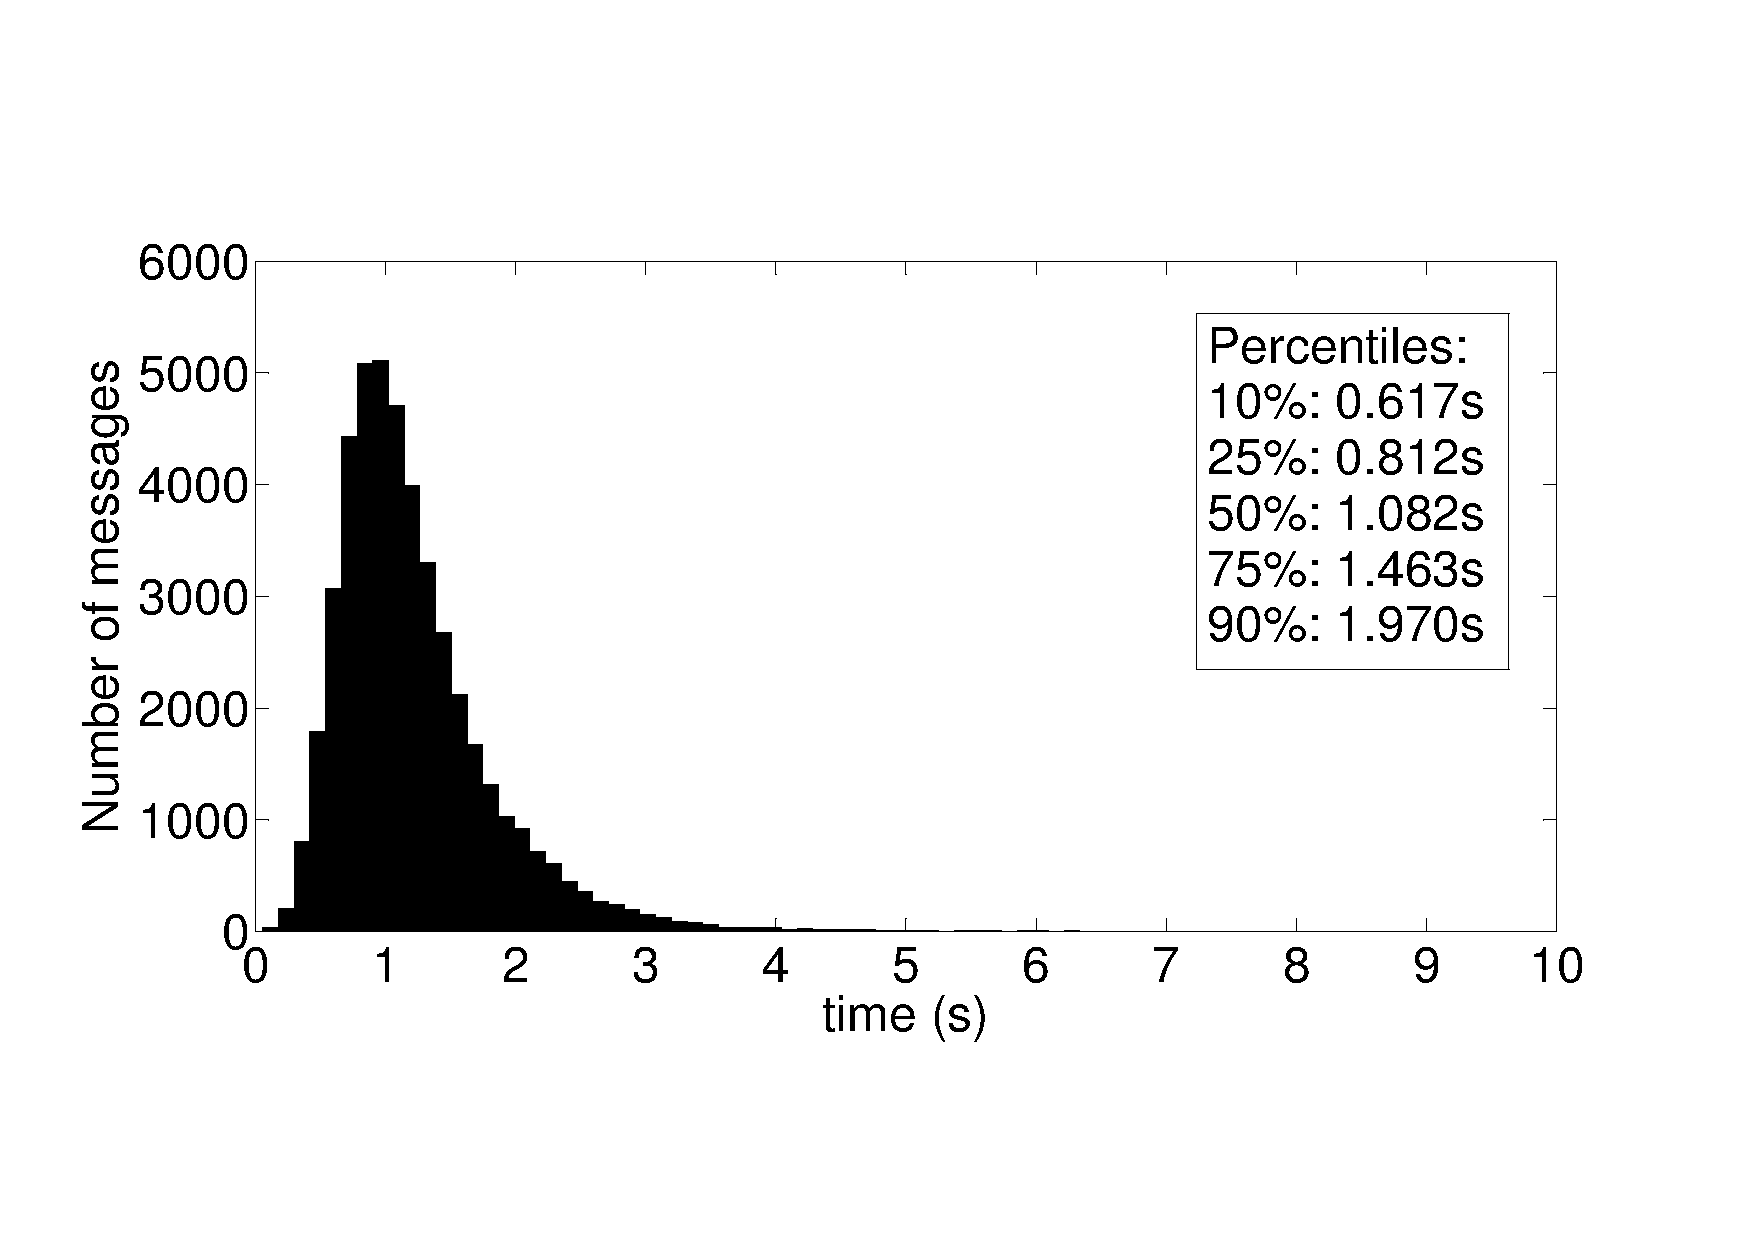
\includegraphics[clip=true, viewport=5mm 65mm 265mm 205mm, width=\columnwidth]{overlay_put_sf}
 \caption{Overlay storage responsiveness}
 \label{fig_overlay_put_sf}
\end{figure}
%
Figure \ref{fig_overlay_put_sf} shows that to store an object in the overlay can take anywhere from 0.1 to 4 seconds.

\begin{figure}[htbp]
 \centering
 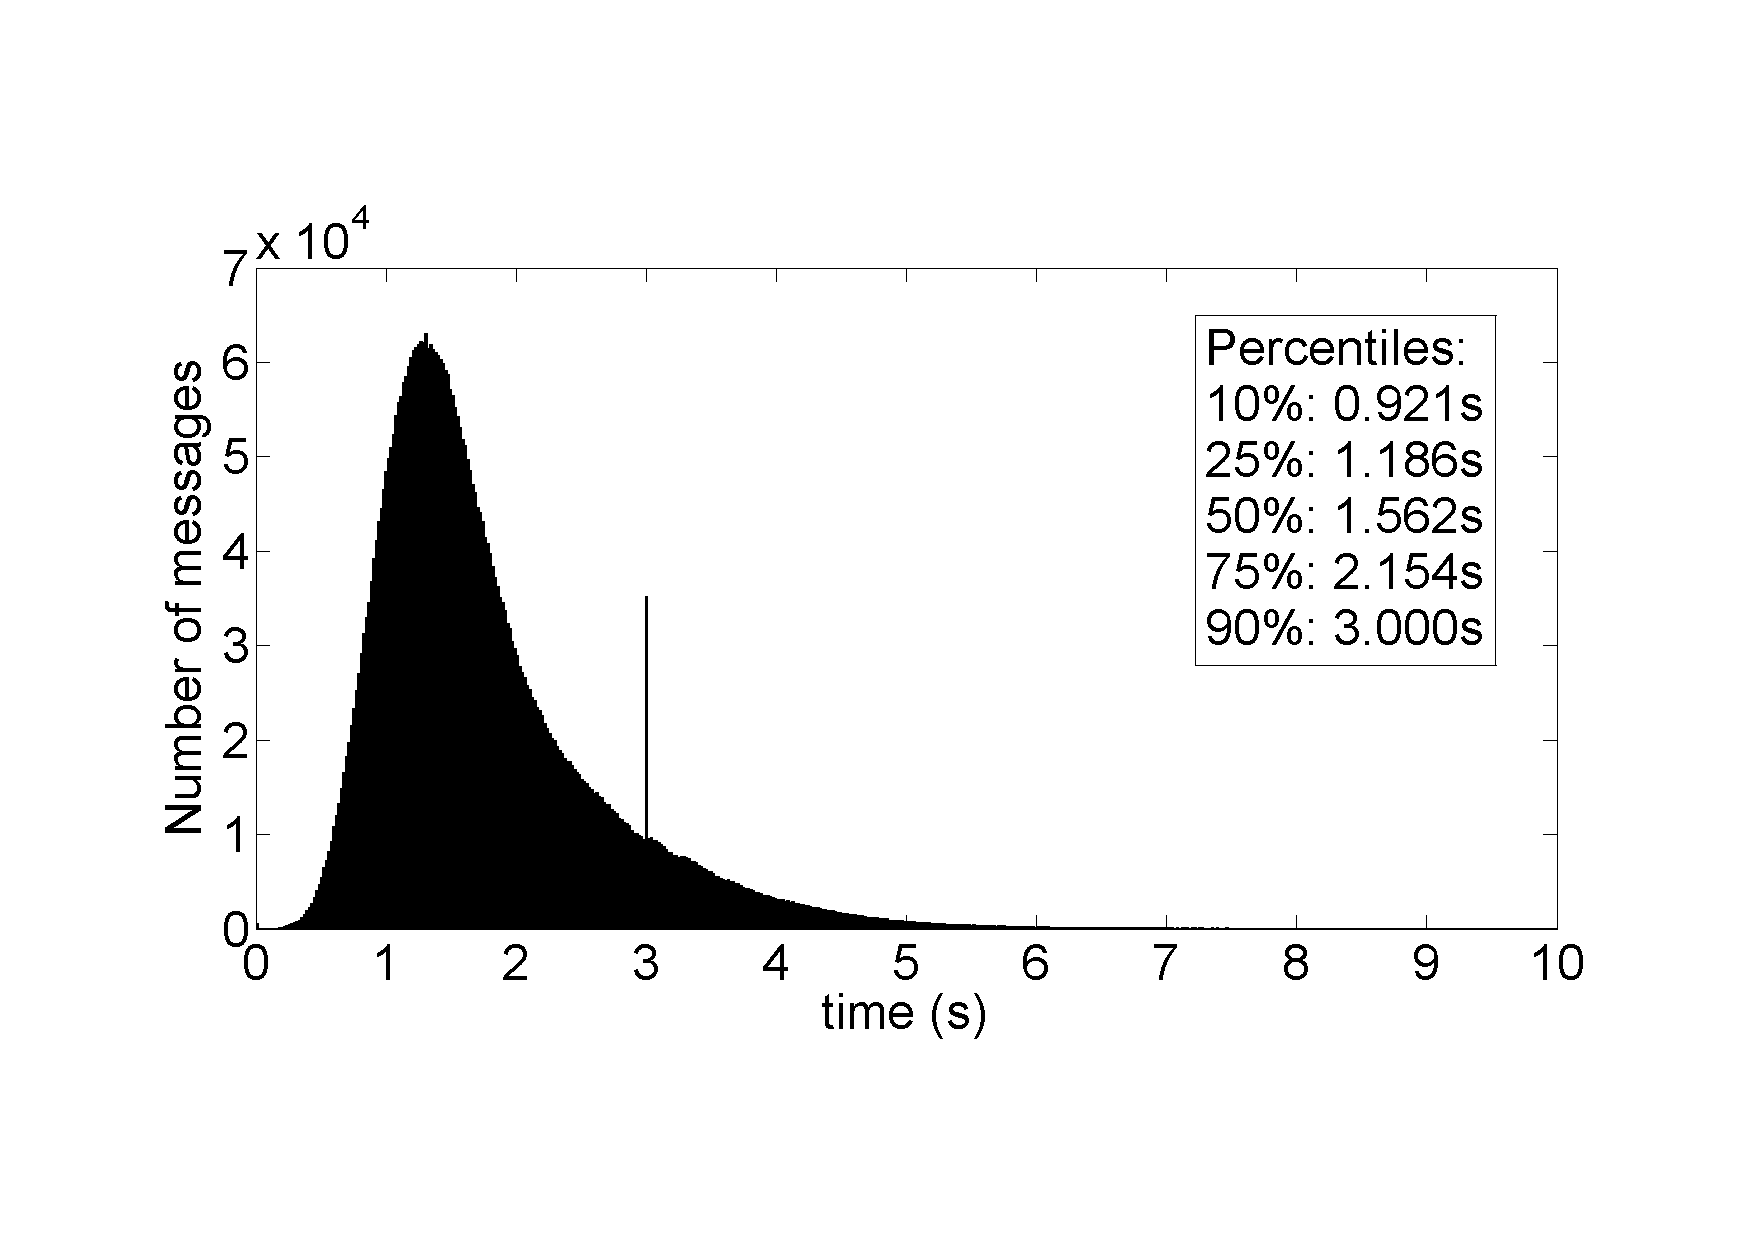
\includegraphics[clip=true, viewport=20mm 30mm 270mm 190mm, width=\columnwidth]{overlay_get_sf}
 \caption{Overlay retrieval responsiveness}
 \label{fig_overlay_get_sf}
\end{figure}
%
Figure \ref{fig_overlay_get_sf} shows that to retrieve an object from the overlay can take anywhere from 0.1 to 6 seconds. Figure \ref{fig_overlay_get_sf} also shows a spike at 3 seconds, when overlay retrieval is performed. This means that a large number of requests take 3 seconds to complete. This is thought to be an artifact of Chord lookup performance due to timeouts as set up in the Oversim simulation.

Overlay storage and retrieval has a high standard deviation when compared to group storage and retrieval as will be shown in the next sections.


\subsection{Group storage}
\label{group_storage_eval}

\subsubsection{Fast storage}
\label{group_put_f_fp}

Figure \ref{fig_group_put_fp} shows the distribution of group storage for fast storage.

\begin{figure}[htbp]
 \centering
 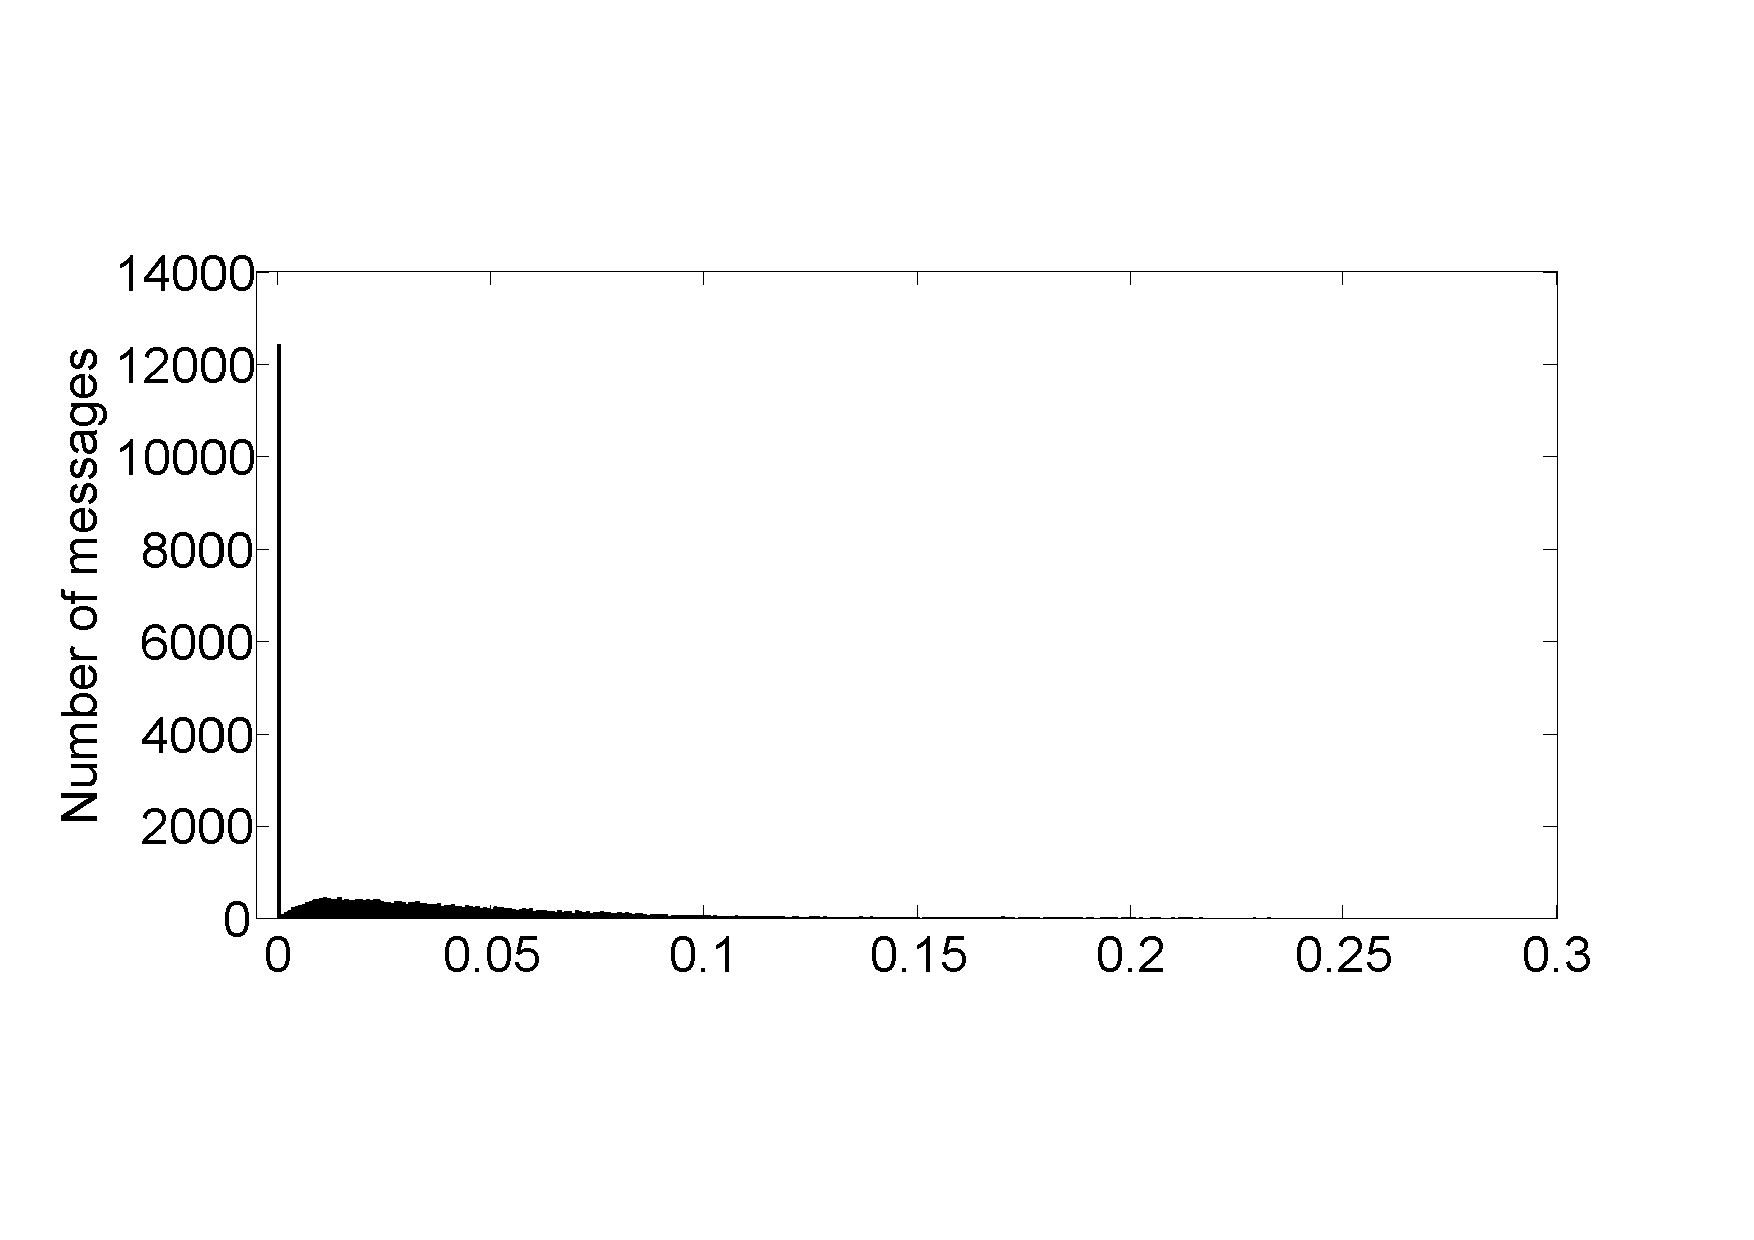
\includegraphics[clip=true, viewport=10mm 30mm 270mm 185mm, width=\columnwidth]{group_put_fp}
 \caption{Group storage responsiveness for fast storage}
 \label{fig_group_put_fp}
\end{figure}
%
Figure \ref{fig_group_put_fp} shows a high peak at close to zero seconds. This peak shows that a large number of storage requests have a small time compared to the rest of requests. These requests are the requests where the node generating the object is chosen to store the object. If the required number of replicas is high, compared to the group size, there is a high likelihood that the node originating the request will be chosen as a host node to the object. This is why there is such a large spike at close to zero.

It should be noted that the node that originally stored the object does not have local access to the object. Only other nodes that did not originally store the object may have access to local copies.

Apart from the spike, Figure \ref{fig_group_put_fp} also shows that the responsiveness is distributed over a small range: from zero to 0.1 seconds.

\subsubsection{Safe storage}
\begin{figure}[htbp]
 \centering
 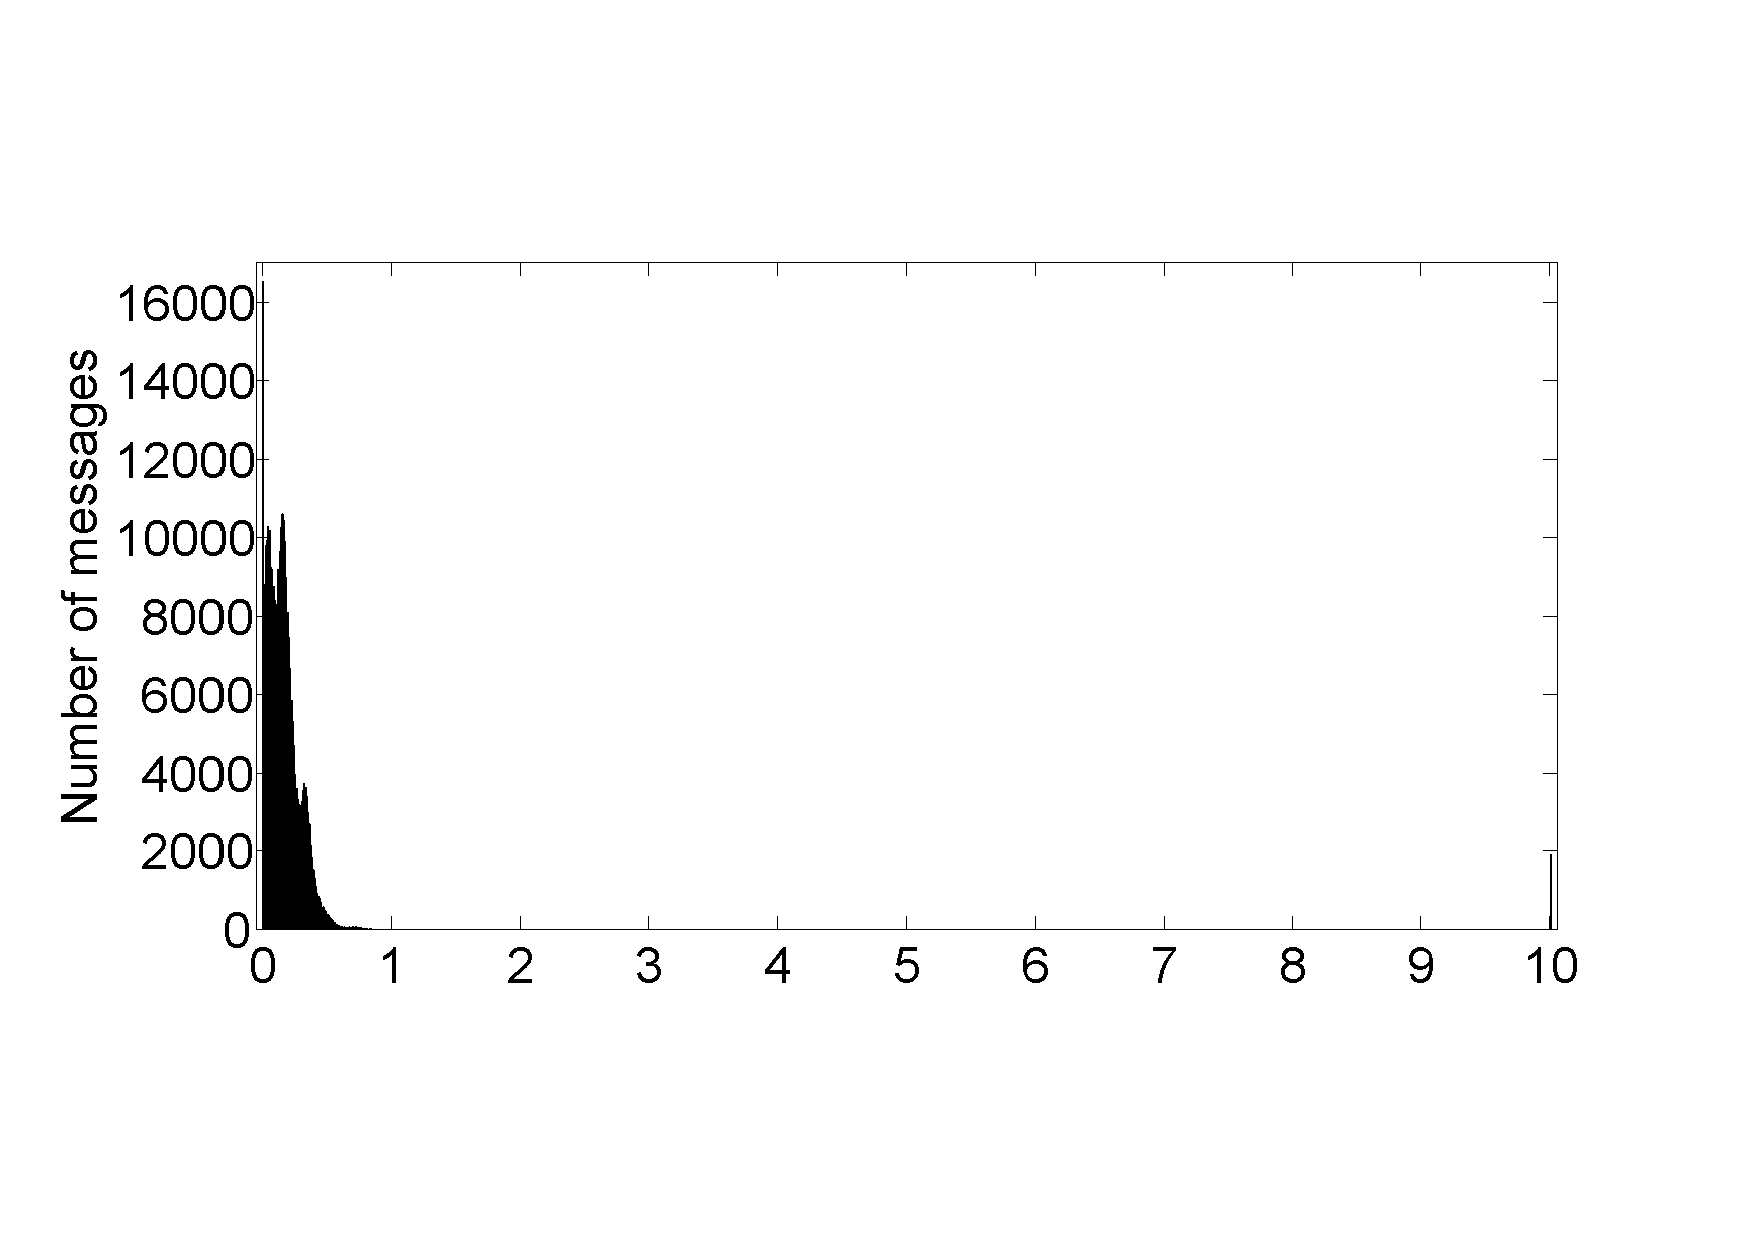
\includegraphics[clip=true, viewport=10mm 30mm 270mm 180mm, width=\columnwidth]{group_put_sf}
 \caption{Group storage responsiveness for safe storage}
 \label{fig_group_put_sf}
\end{figure}
%
Figure \ref{fig_group_put_sf} shows the responsiveness distribution for safe storage. Because safe storage is slower than fast storage, the mean response time is longer. The maximum and minimum responsiveness values are also greater than for fast storage: from zero to 0.8 seconds. This is still smaller than the range of overlay storage values.

Figure \ref{fig_group_put_sf} also contains a spike at 10s. This is due to the storage timeout being set to 10s. What should be noted is that these responsiveness graphs shows both success and failure responsiveness. In other words, it shows how quickly a response is received, even if that response is a failure. The responses received from 10 s will all be failures, where no response was received from the destination node and an internal timeout occurred.

The ``bumps'' in Figure \ref{fig_group_put_sf} are similar to the ones seen in group retrieval in Figure \ref{fig_group_get_zoom_sf} and are artifacts of Oversim's SimpleUnderlay network structure, as discussed in Section \ref{lan_retrieval}. The large spike at zero seconds is also present for the same reason mentioned earlier.

\subsection{Group retrieval}
\subsubsection{Fast retrieval and safe or fast storage}
\begin{figure}[htbp]
 \centering
 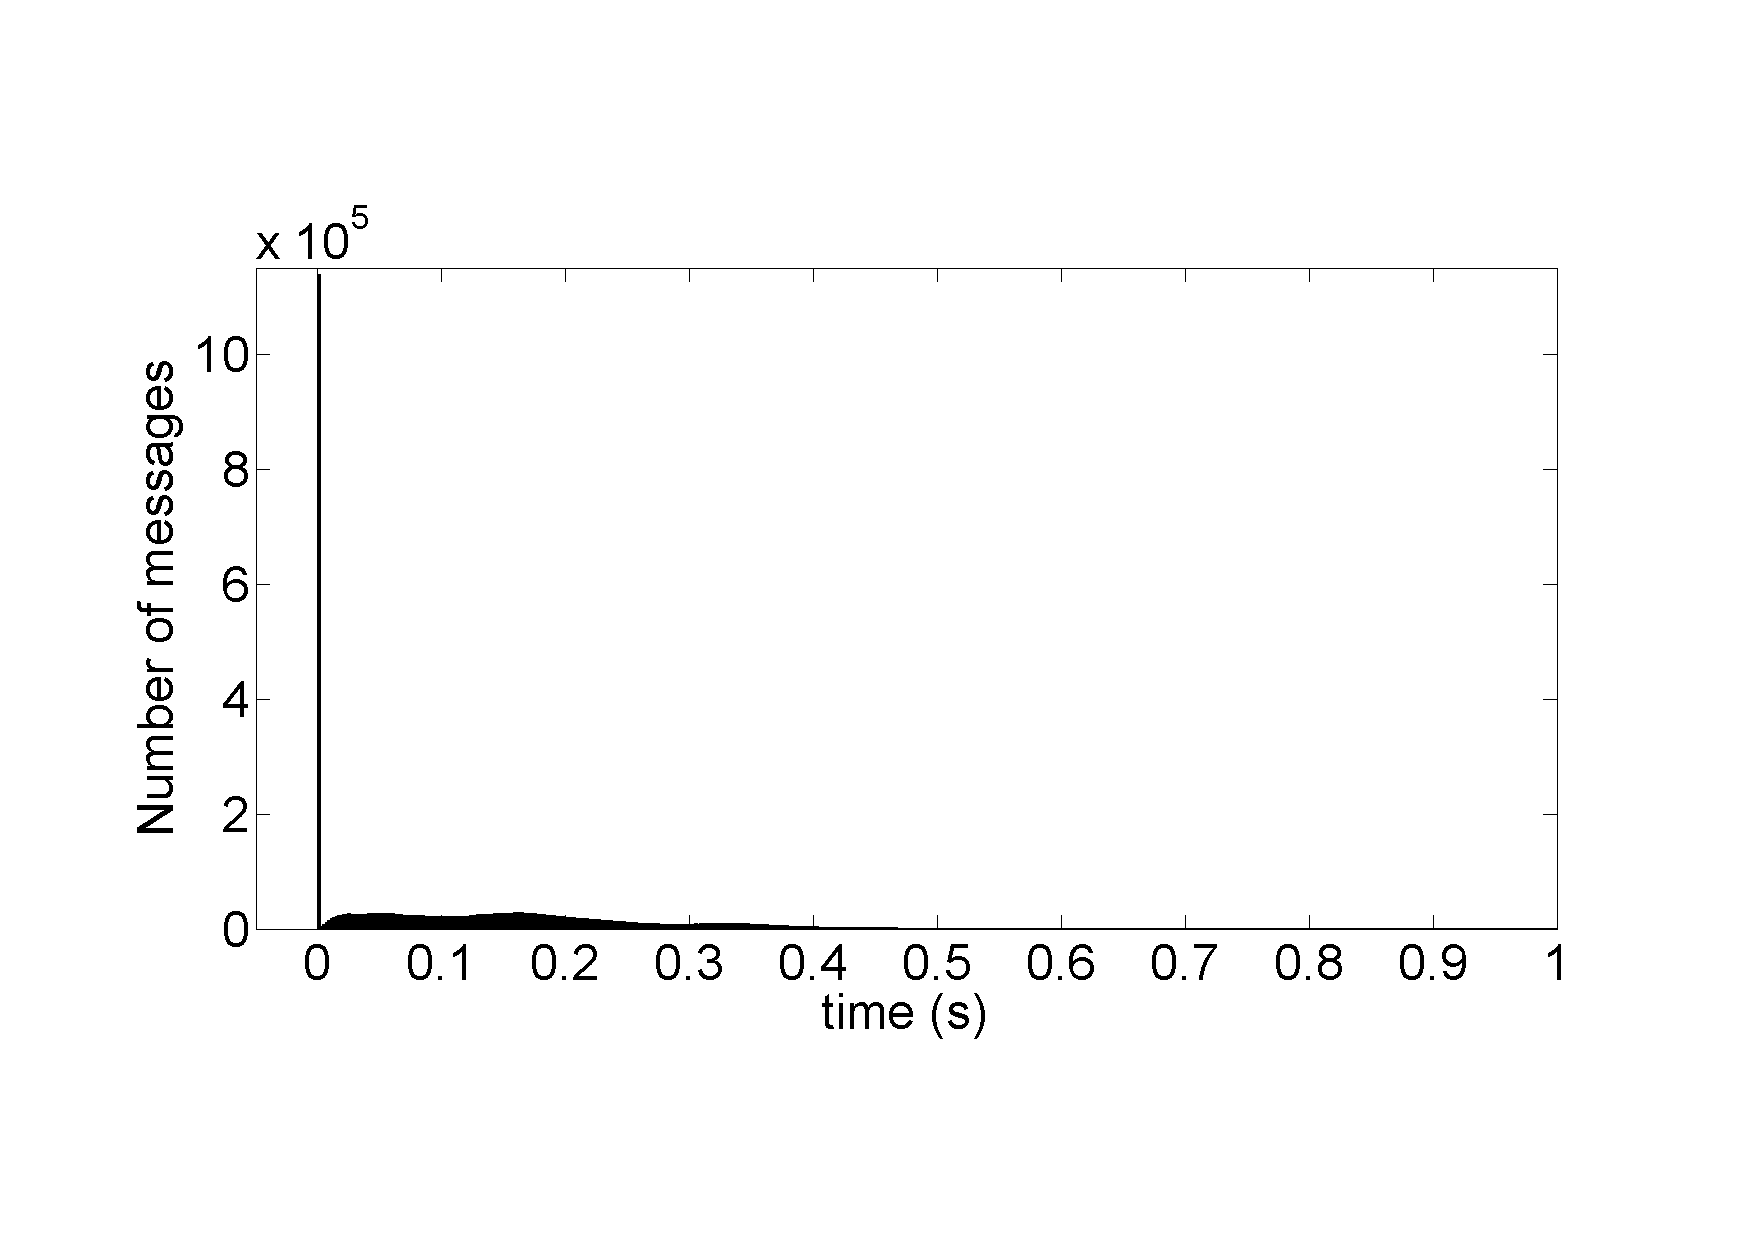
\includegraphics[clip=true, viewport=20mm 30mm 265mm 180mm, width=\columnwidth]{group_get_sf}
 \caption{Group retrieval responsiveness for safe or fast storage and fast retrieval}
 \label{fig_group_get_sf}
\end{figure}
%
Figure \ref{fig_group_get_sf} shows group retrieval responsiveness for fast retrieval and safe or fast storage. This type of retrieval also shows a spike at zero seconds due to nodes requesting objects from the network and those objects being found in the locally stored root object store. Because of the high number of replicas compared to the average group size used in the simulation, many of the requests can be locally served, which greatly increases responsiveness.

\begin{figure}[htbp]
 \centering
 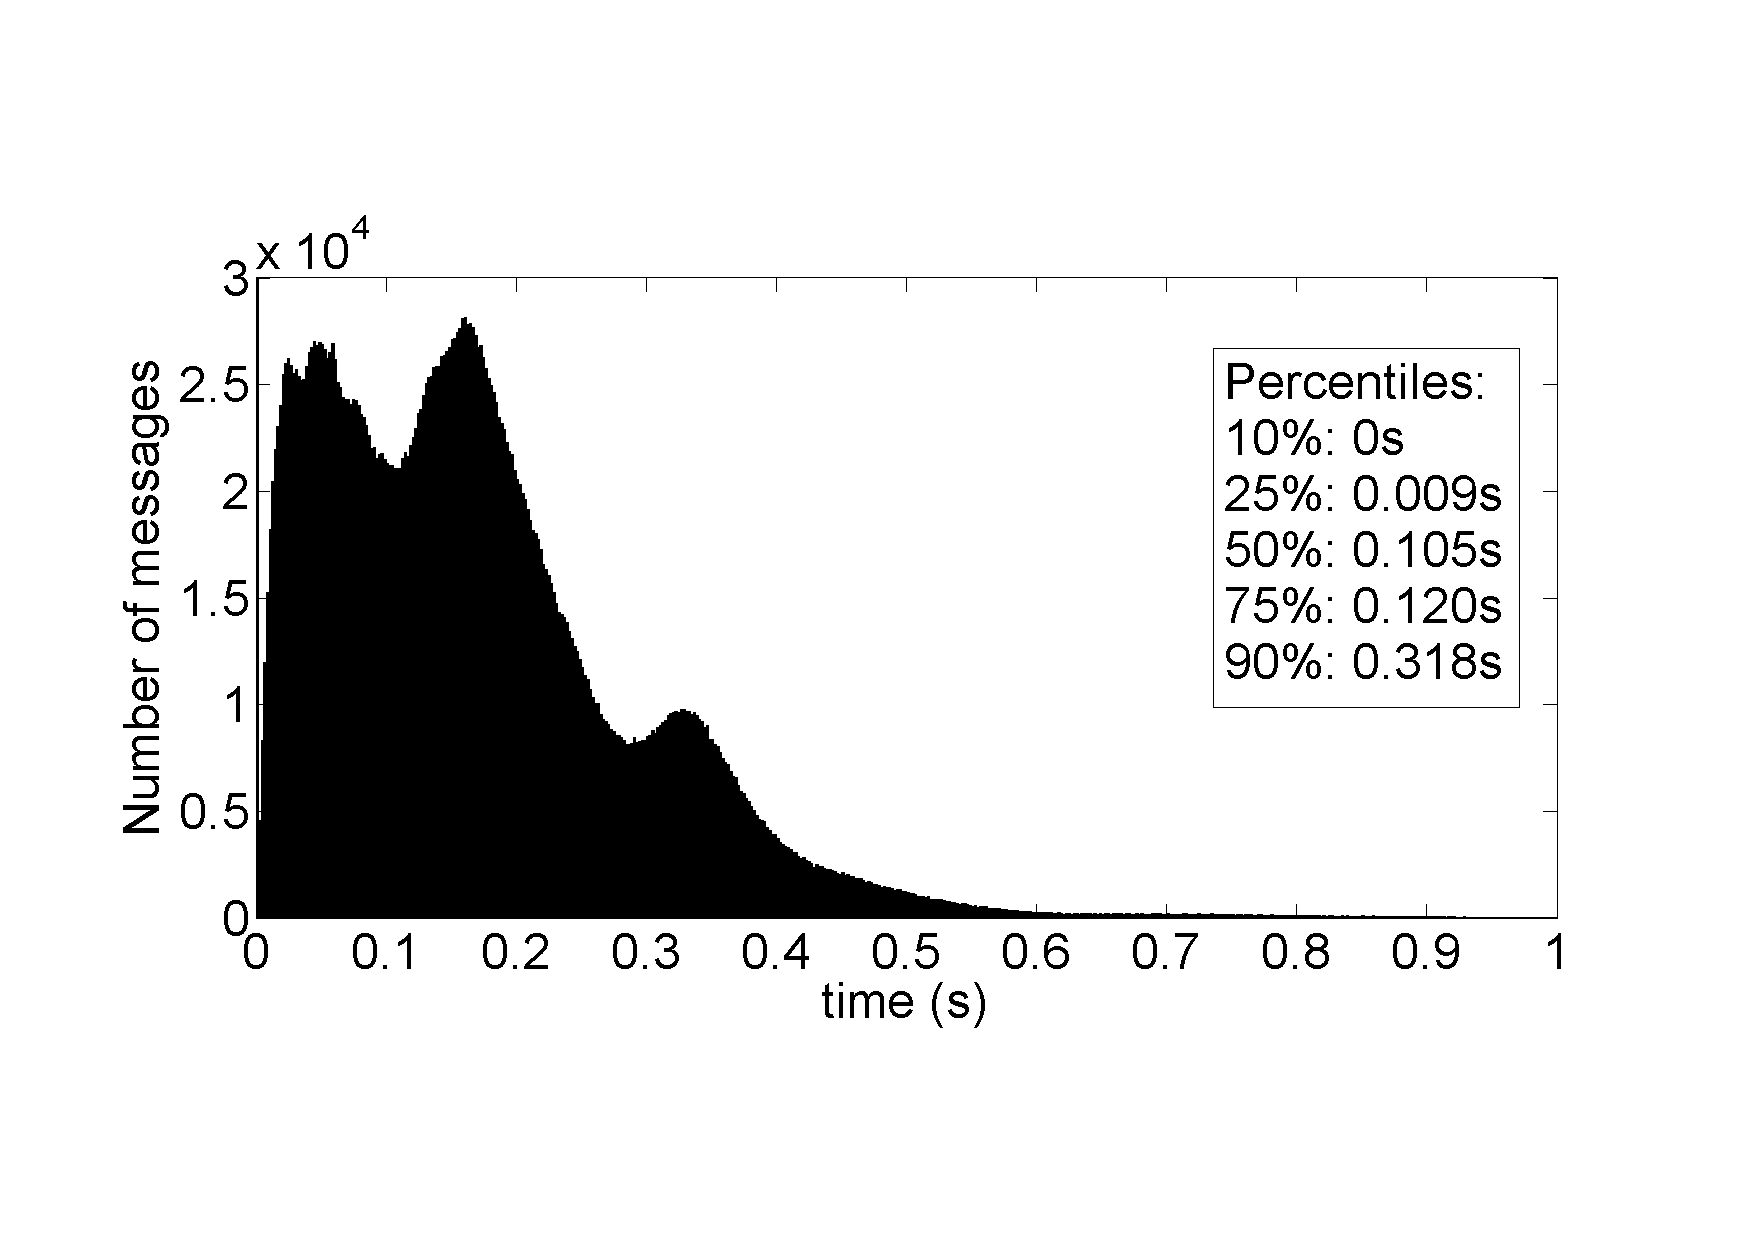
\includegraphics[clip=true, viewport=20mm 30mm 265mm 180mm, width=\columnwidth]{group_get_zoom_sf}
 \caption{Enlarged view of the group retrieval responsiveness for safe or fast storage and fast retrieval}
 \label{fig_group_get_zoom_sf}
\end{figure}
%
The details of Figure \ref{fig_group_get_sf} can clearly be seen in Figure \ref{fig_group_get_zoom_sf}, which presents an enlarged view of Figure \ref{fig_group_get_sf}. This figure also shows the multiple ``bumps'', which is an artifact of the underlying physical layer, as described in Section \ref{lan_retrieval}. The figure shows that fast group retrieval responsiveness varies from zero to 0.9 seconds.

\subsubsection{Parallel retrieval and safe or fast storage}
\begin{figure}[htbp]
 \centering
 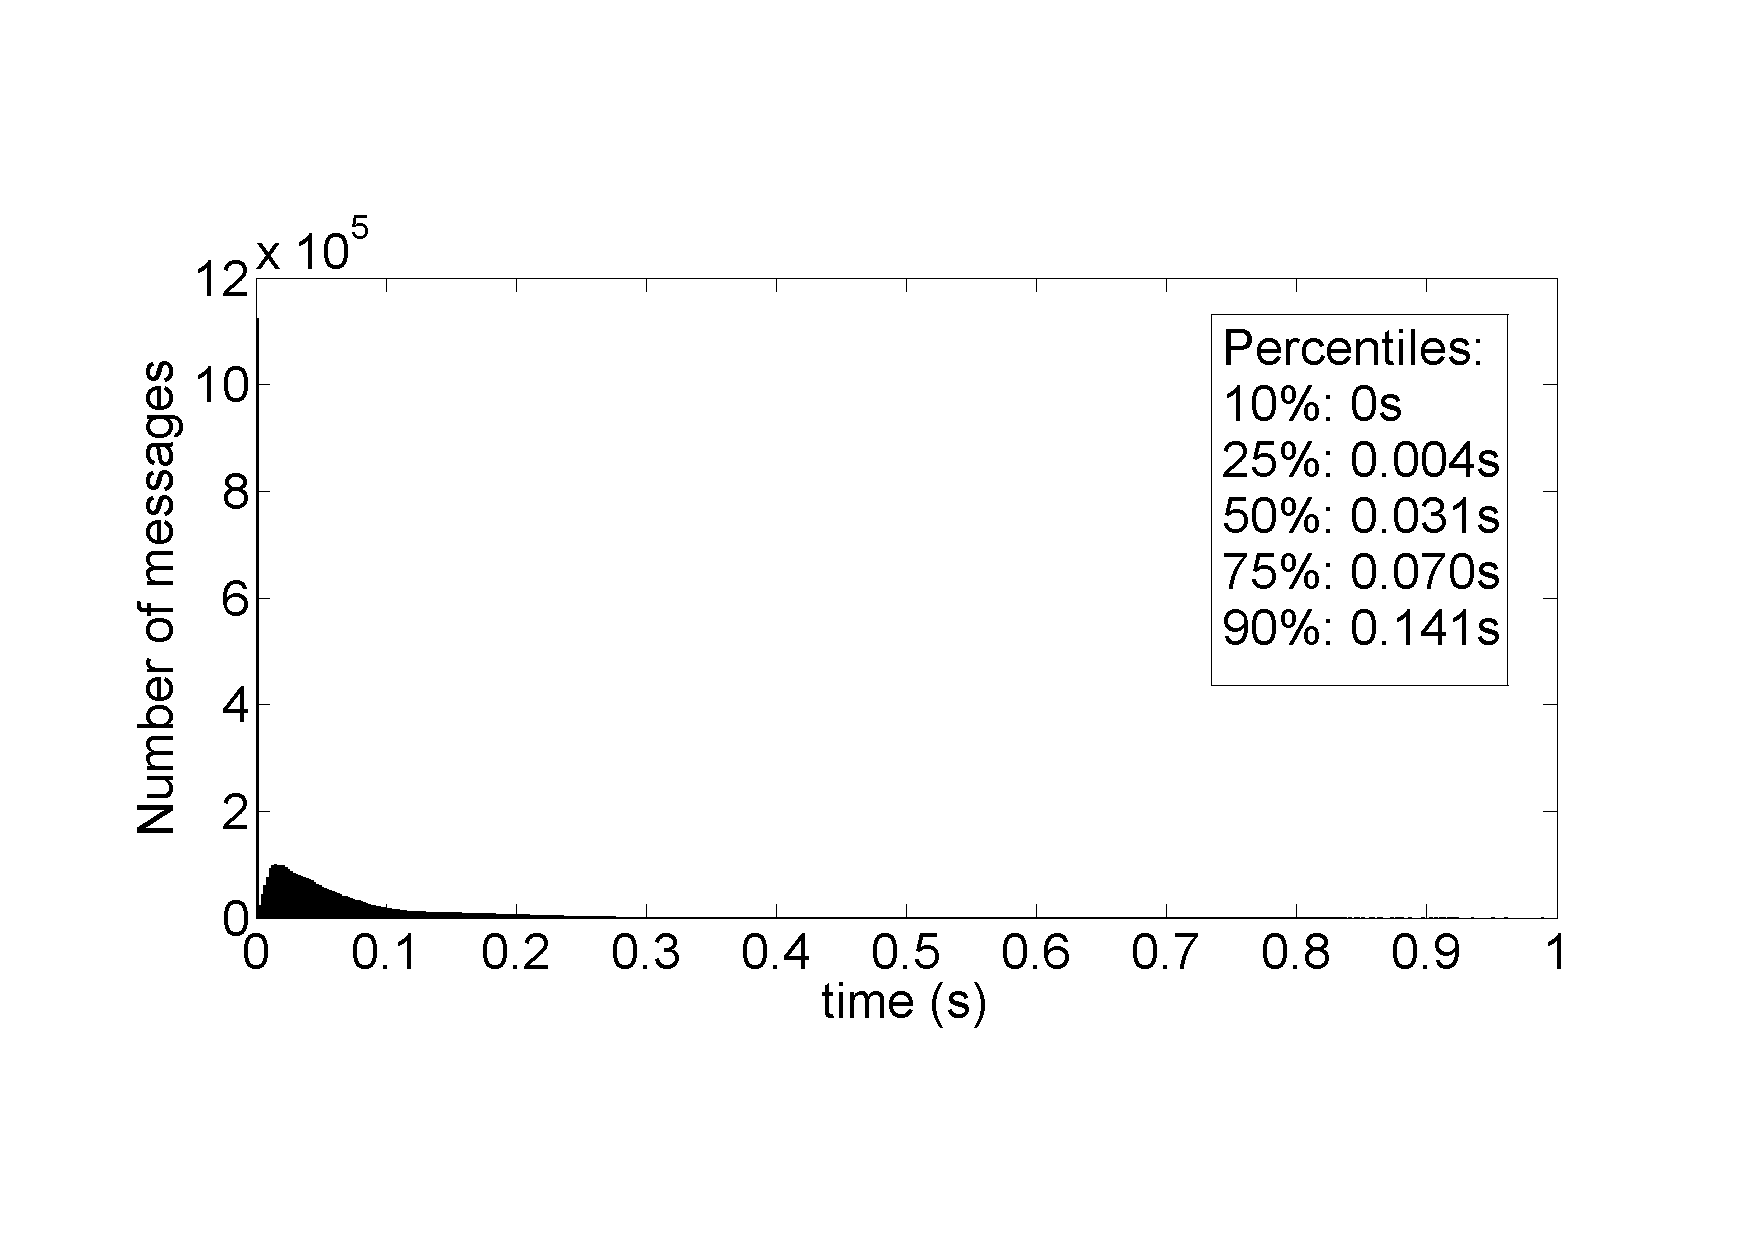
\includegraphics[clip=true, viewport=20mm 30mm 265mm 180mm, width=\columnwidth]{group_get_fp}
 \caption{Group retrieval responsiveness for safe or fast storage and parallel retrieval}
 \label{fig_group_get_fp}
\end{figure}

\begin{figure}[htbp]
 \centering
 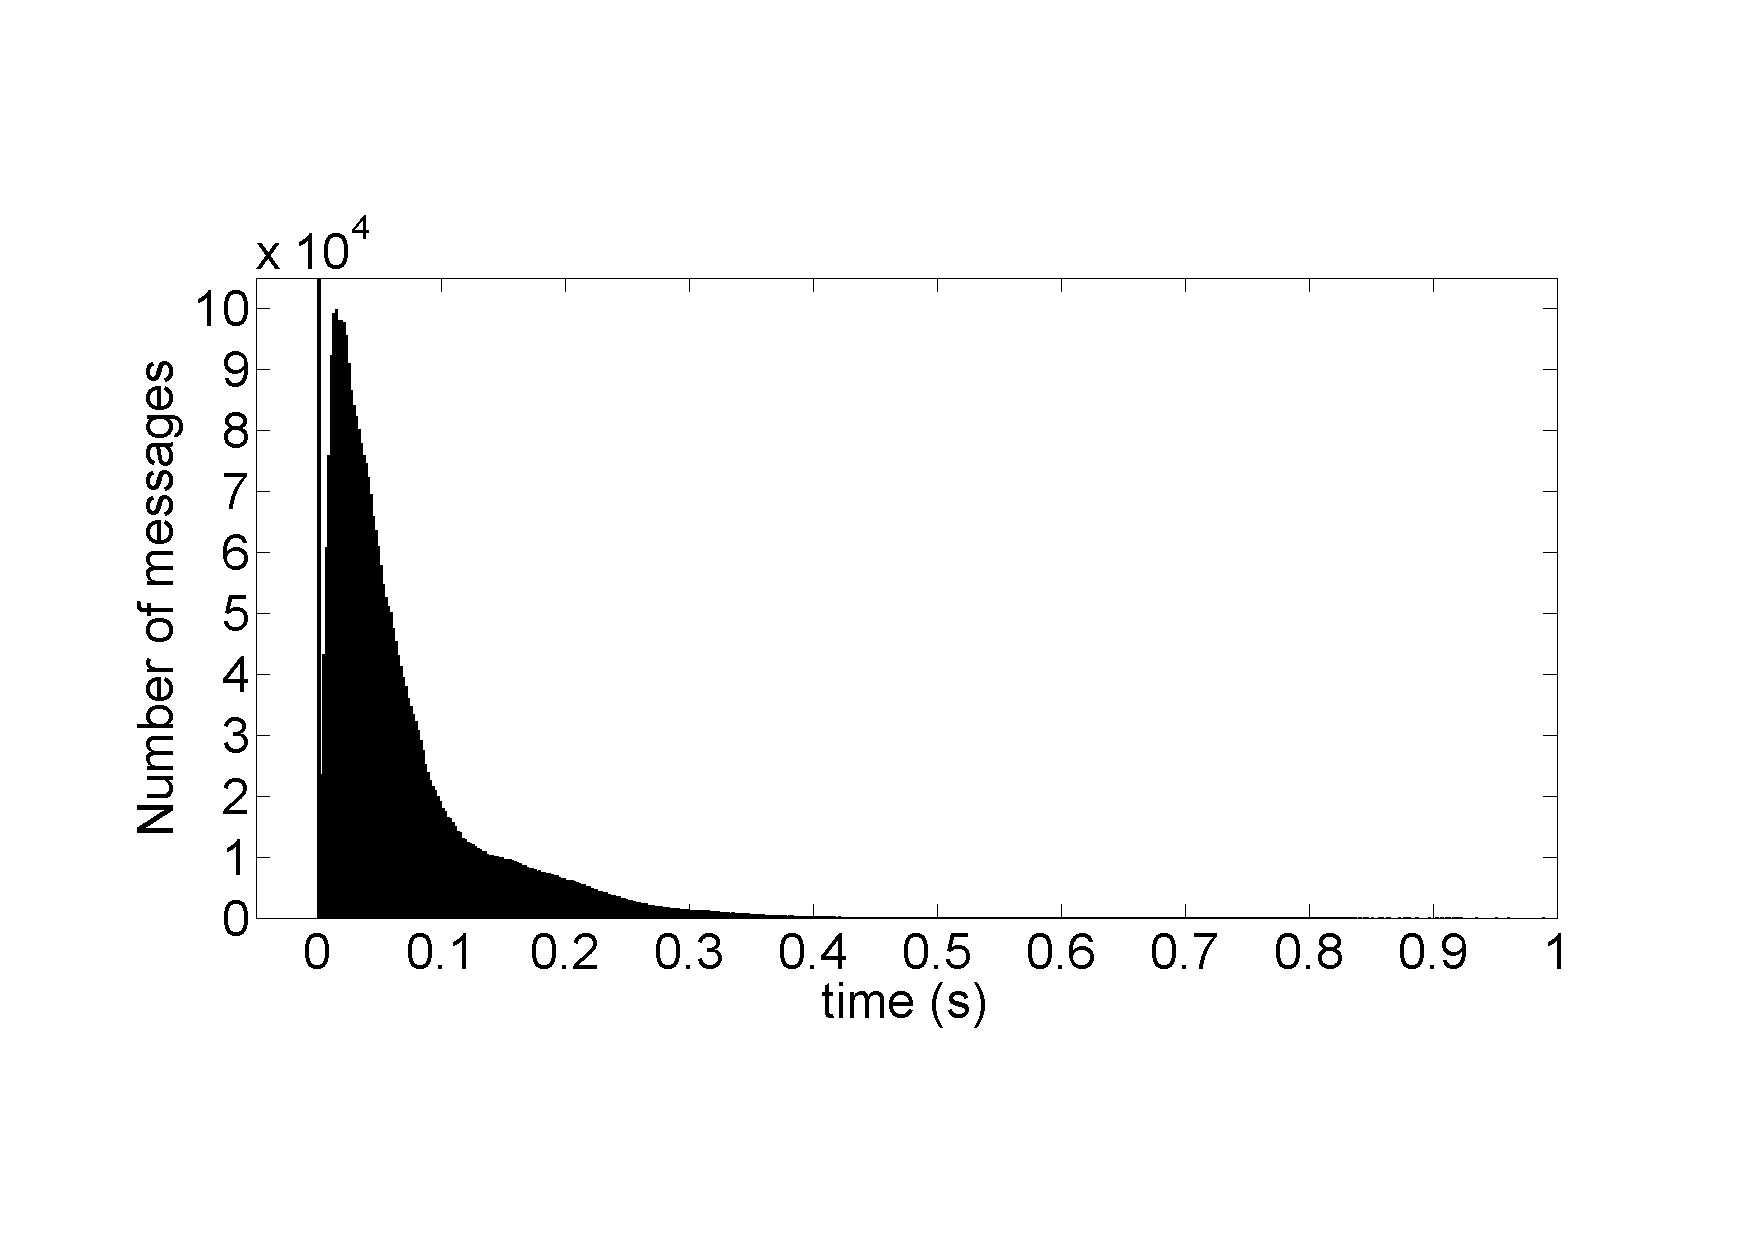
\includegraphics[clip=true, viewport=20mm 30mm 265mm 180mm, width=\columnwidth]{group_get_zoom_fp}
 \caption{Enlarged view of the group retrieval responsiveness for safe or fast storage and parallel retrieval}
 \label{fig_group_get_zoom_fp}
\end{figure}
%
Figure \ref{fig_group_get_fp} shows group retrieval responsiveness for parallel retrieval and fast or safe storage and Figure \ref{fig_group_get_zoom_fp} shows the enlarged view. Apart from the higher responsiveness, explained in Section \ref{pithos_resp_rel_results}, parallel retrieval also has a smaller range of values: from zero to 0.4 seconds.

The shape of Figure \ref{fig_group_get_zoom_fp} differs from that of Figure \ref{fig_group_get_zoom_sf} due to the difference between selecting a single random node ($1/r$) in the group for retrieval, to selecting the fastest of $r$ nodes in the group for retrieval, where $r$ is the number of object replicas currently in the group.

\subsection{LAN performance}
\label{lan_retrieval}

Figures \ref{fig_group_put_sf} and \ref{fig_group_get_zoom_sf} show ``bumps'' that were described as being underlying network artifacts. To show that this, another simulation run is performed where the coordinate-based system used in Oversim is replaced by all links being set to have 1ms latency and jitter of 0.1\%. The purpose of this is to show that group storage has the correct expected number of hops, that the ``bumps'' are not inherent to Pithos and that Pithos's performance is greatly improved when the underlaying network architecture has improved performance.

\begin{figure}[htbp]
 \centering
 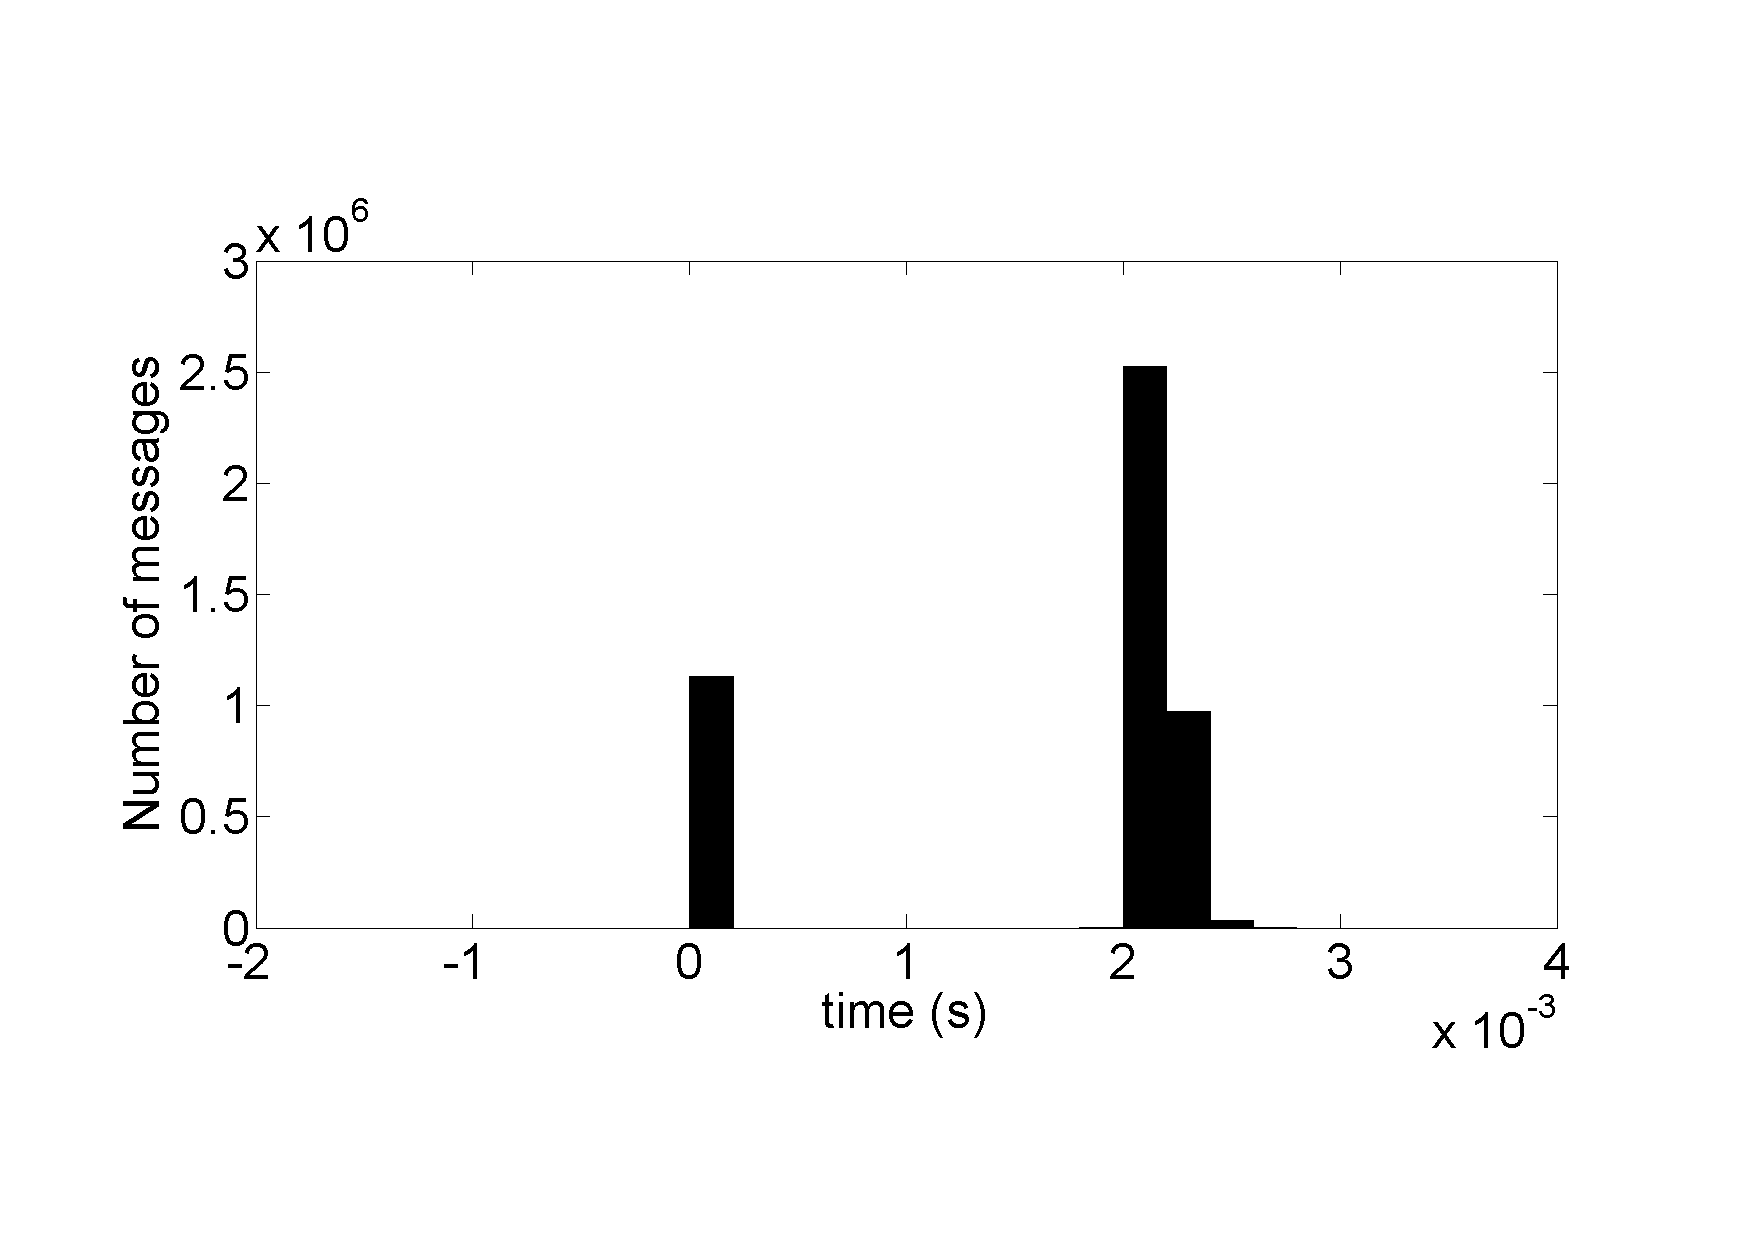
\includegraphics[clip=true, viewport=20mm 30mm 265mm 180mm, width=\columnwidth]{group_get_lan}
 \caption{Group retrieval responsiveness for fast storage and fast retrieval, running on a 1ms underlay network.}
 \label{fig_group_get_lan}
\end{figure}
%
Figure \ref{fig_group_get_lan} shows group retrieval performance for fast storage and fast retrieval, running on a 1ms underlay network. This figure shows the same operation shown in Figure \ref{fig_group_get_zoom_sf}, but for the underlay being a fixed 1ms underlay, instead of a coordinate-based underlay.

Two main spikes are seen in the figure, one at 0s and another at 2ms. There are no other measured times. This is what is expected from group storage, since every request in group storage is zero hops or two hope. For two hops, one hop is required to sent the request, and another to receive the response, which gives $2\times 1 ms = 2 ms$. The zero hops case was explained in Section \ref{group_put_f_fp}.

No additional spikes are perceived, as opposed to the ``bumps'' seen earlier. The mean group storage performance has improved to 1.6ms, from the 192ms for the coordinate-based underlay network.

\subsection{Overall storage}

\subsubsection{Fast storage and fast or parallel retrieval}
After having presented the separate responsiveness profiles for overlay and group storage, the overall Pithos responsiveness is presented here which is a combination of the responsiveness profiles of the underlying group and overlay responsiveness.

\begin{figure}[htbp]
 \centering
 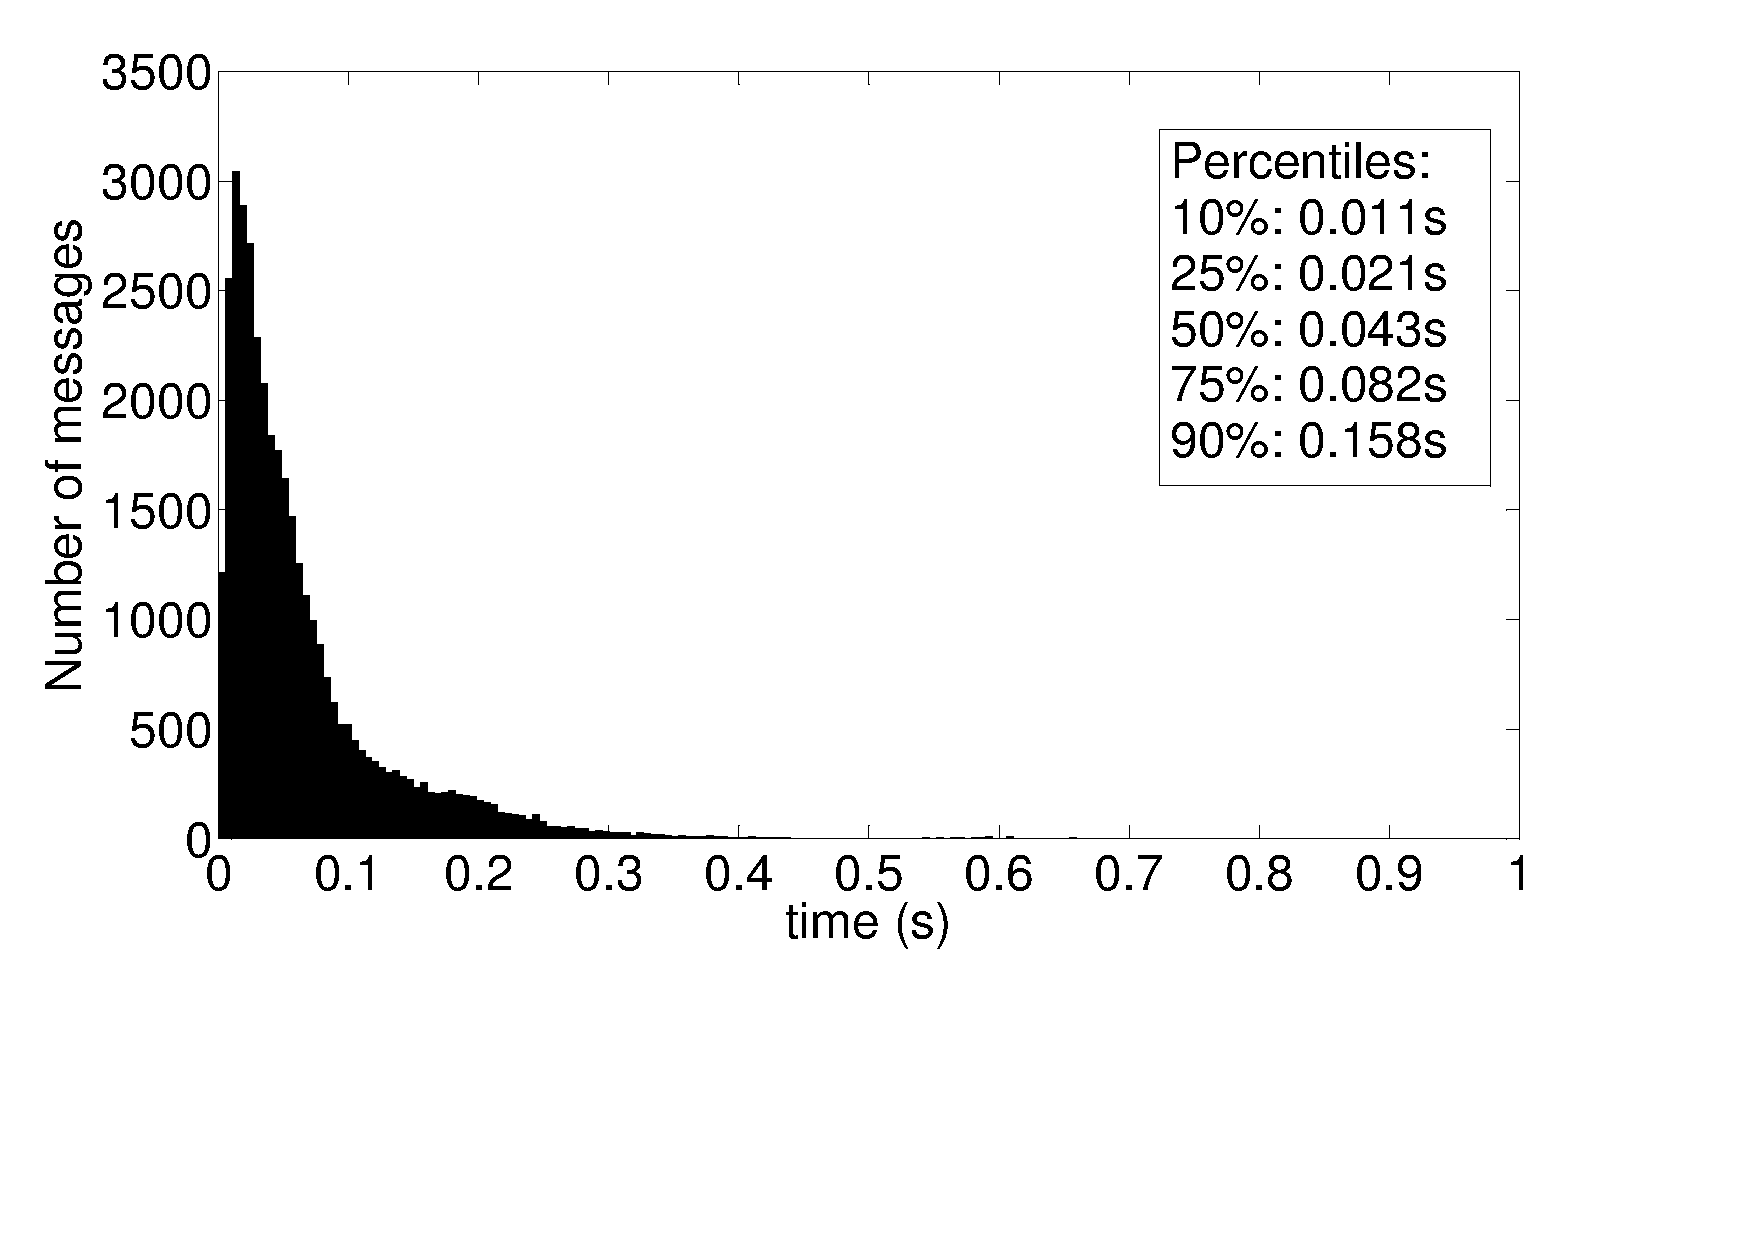
\includegraphics[clip=true, viewport=5mm 35mm 265mm 190mm, width=\columnwidth]{overall_put_ff}
 \caption{Overall storage responsiveness for fast storage and fast or parallel retrieval}
 \label{fig_overall_put_ff}
\end{figure}
%
Figure \ref{fig_overall_put_ff} shows the overall storage responsiveness for fast storage and fast or parallel retrieval. The shape is similar to that of Figure \ref{fig_group_get_zoom_fp}. A seemingly exponential distribution, due to the first successful storage response from group storage being sent to the higher layer. This has the effect of taking all responses and choosing the fastest one. Exactly the same mechanism as with parallel retrieval. Fast storage responsiveness ranges from zero to 0.3 seconds.

\subsubsection{Safe storage and fast or parallel retrieval}
\begin{figure}[htbp]
 \centering
 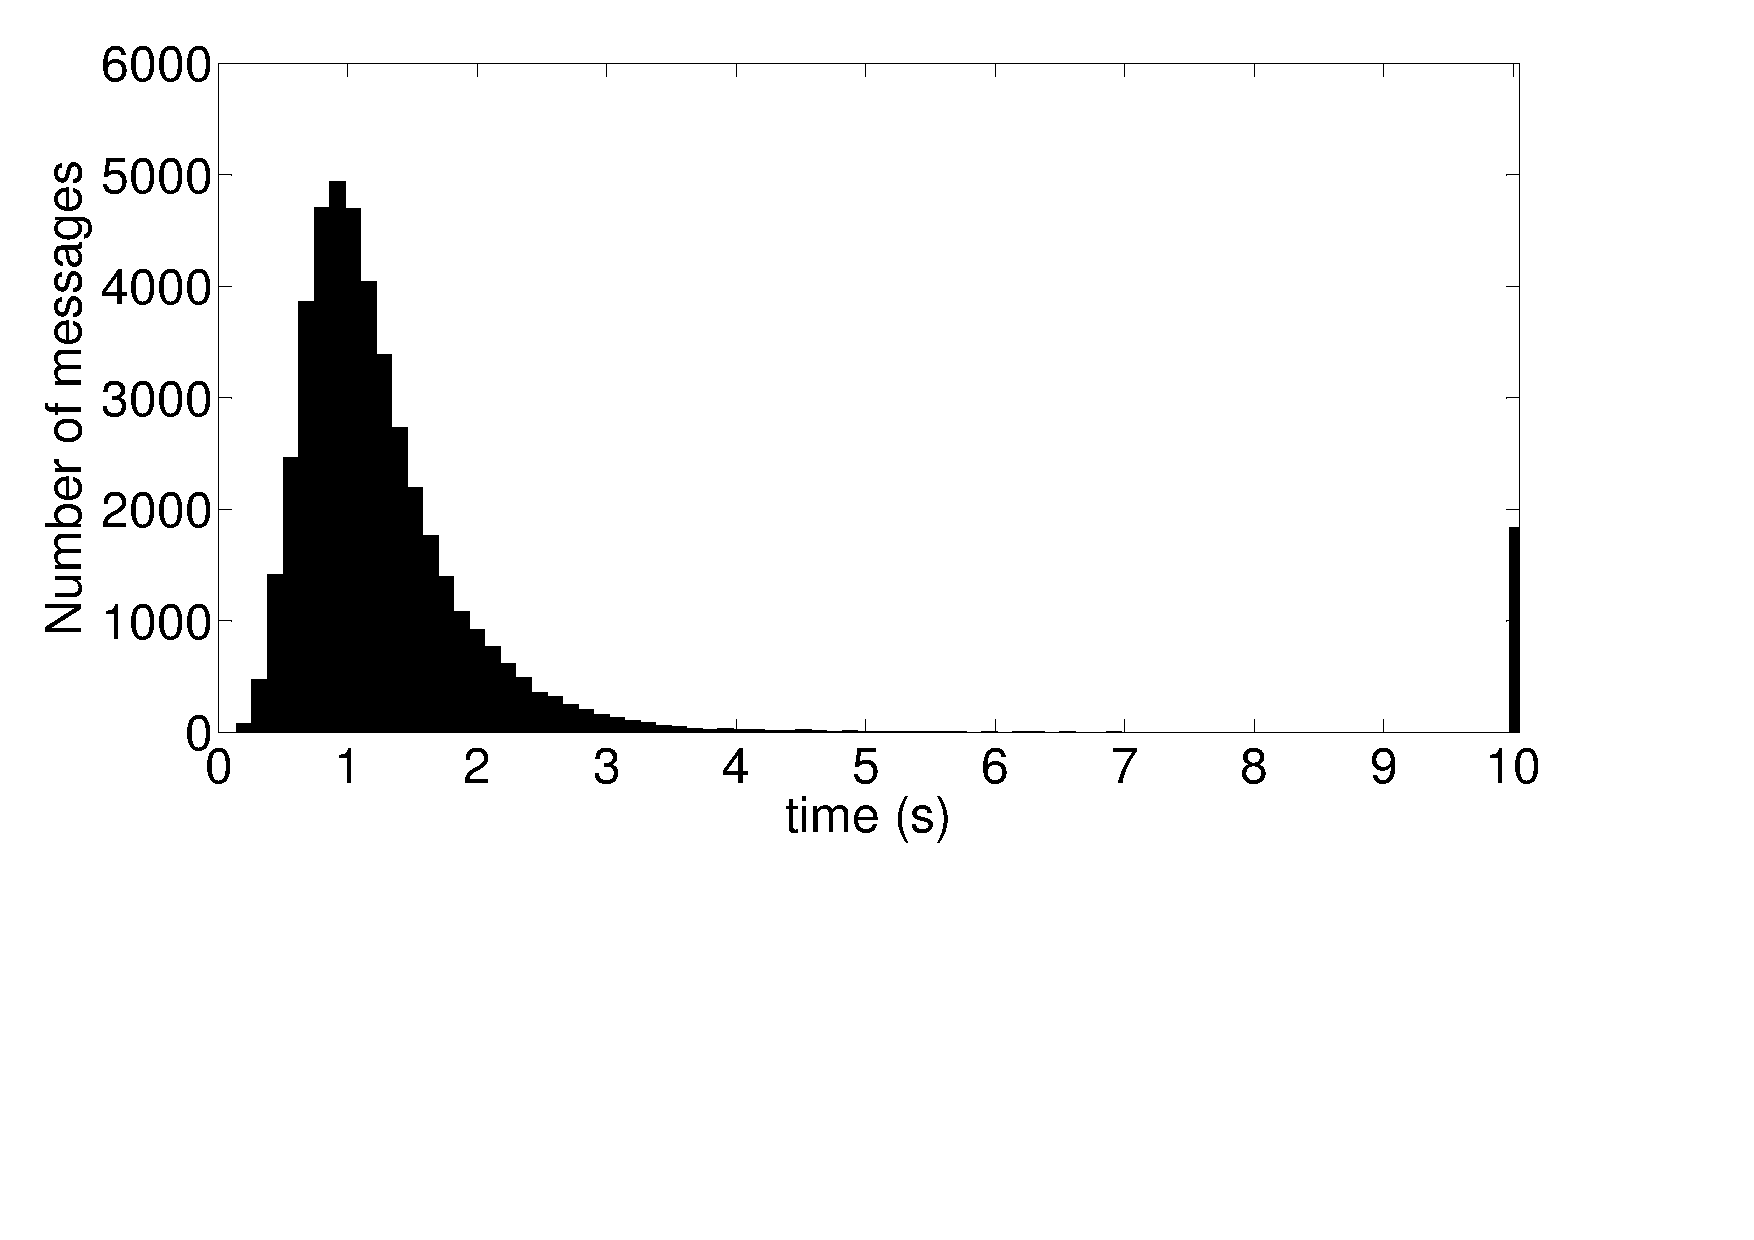
\includegraphics[clip=true, viewport=5mm 60mm 265mm 205mm, width=\columnwidth]{overall_put_sf}
 \caption{Overall storage responsiveness for safe storage and fast or parallel retrieval}
 \label{fig_overall_put_sf}
\end{figure}
%
Figure \ref{fig_overall_put_sf} shows the overall safe storage distribution for fast or parallel retrieval. Because a response is only sent from the group and overlay storage modules to the peer logic module when sufficiently many group responses have been received and when the overlay response has been received, the distribution takes on a shape exactly like the overlay storage distribution of Figure \ref{fig_overlay_put_sf}.

The reason why the shape has no correspondence to group storage responsiveness is because, as previously shown, overlay storage is always slower than group storage. Because safe storage always waits for the reply from the overlay storage module, it has the same shape and values as overlay storage.

\subsection{Overall retrieval}
\subsubsection{Fast retrieval and safe or fast storage}
\begin{figure}[htbp]
 \centering
 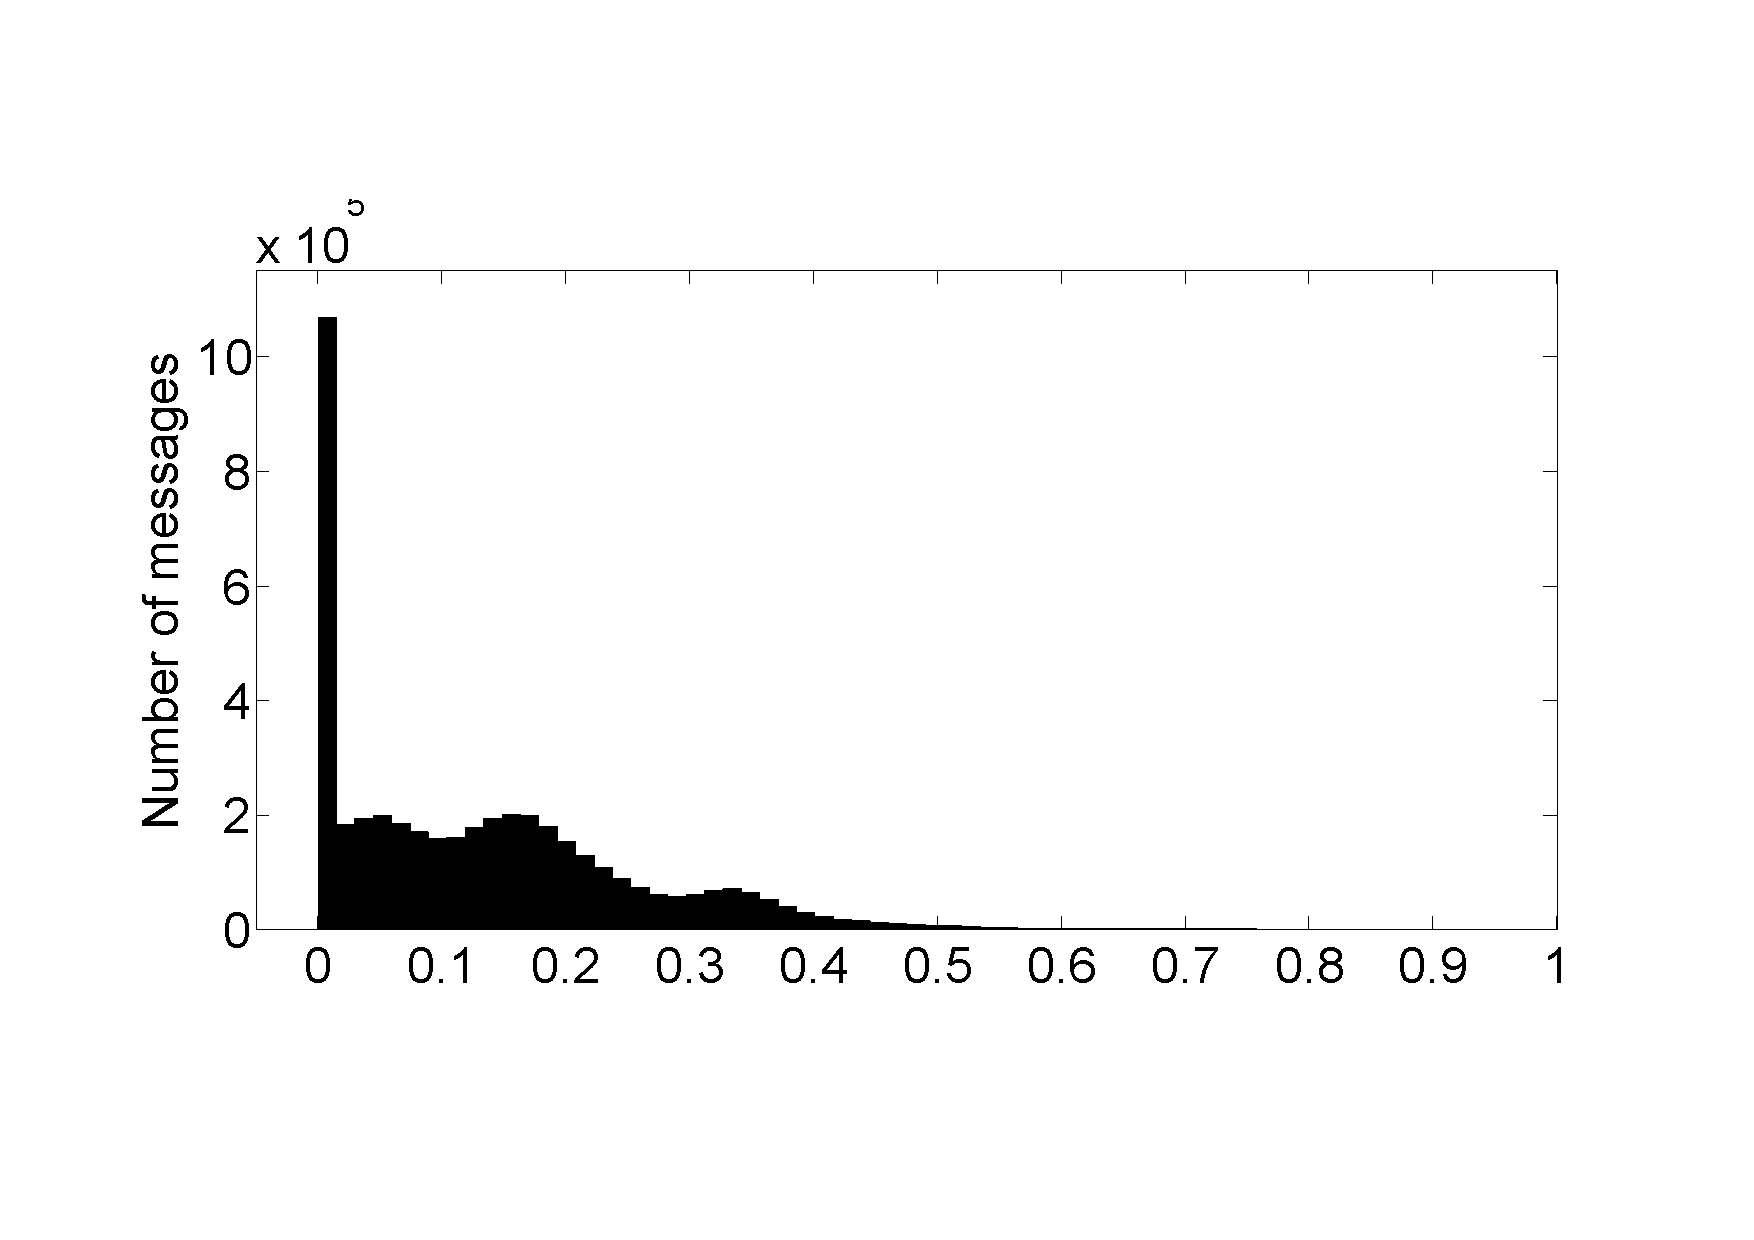
\includegraphics[clip=true, viewport=20mm 30mm 265mm 180mm, width=\columnwidth]{overall_get_ff}
 \caption{Overall retrieval responsiveness for safe or fast storage and fast retrieval}
 \label{fig_overall_get_ff}
\end{figure}
%
Figure \ref{fig_overall_get_ff} shows overall retrieval responsiveness for fast retrieval and safe or fast storage. The shape is similar to that of fast group retrieval in Figure \ref{fig_group_get_sf}, because in this case, fast retrieval returns the first result received. Since fast group retrieval is mostly faster then overlay retrieval, the overall retrieval distribution will closely match that of fast group retrieval.

\subsubsection{Parallel retrieval and safe or fast storage}
\begin{figure}[htbp]
 \centering
 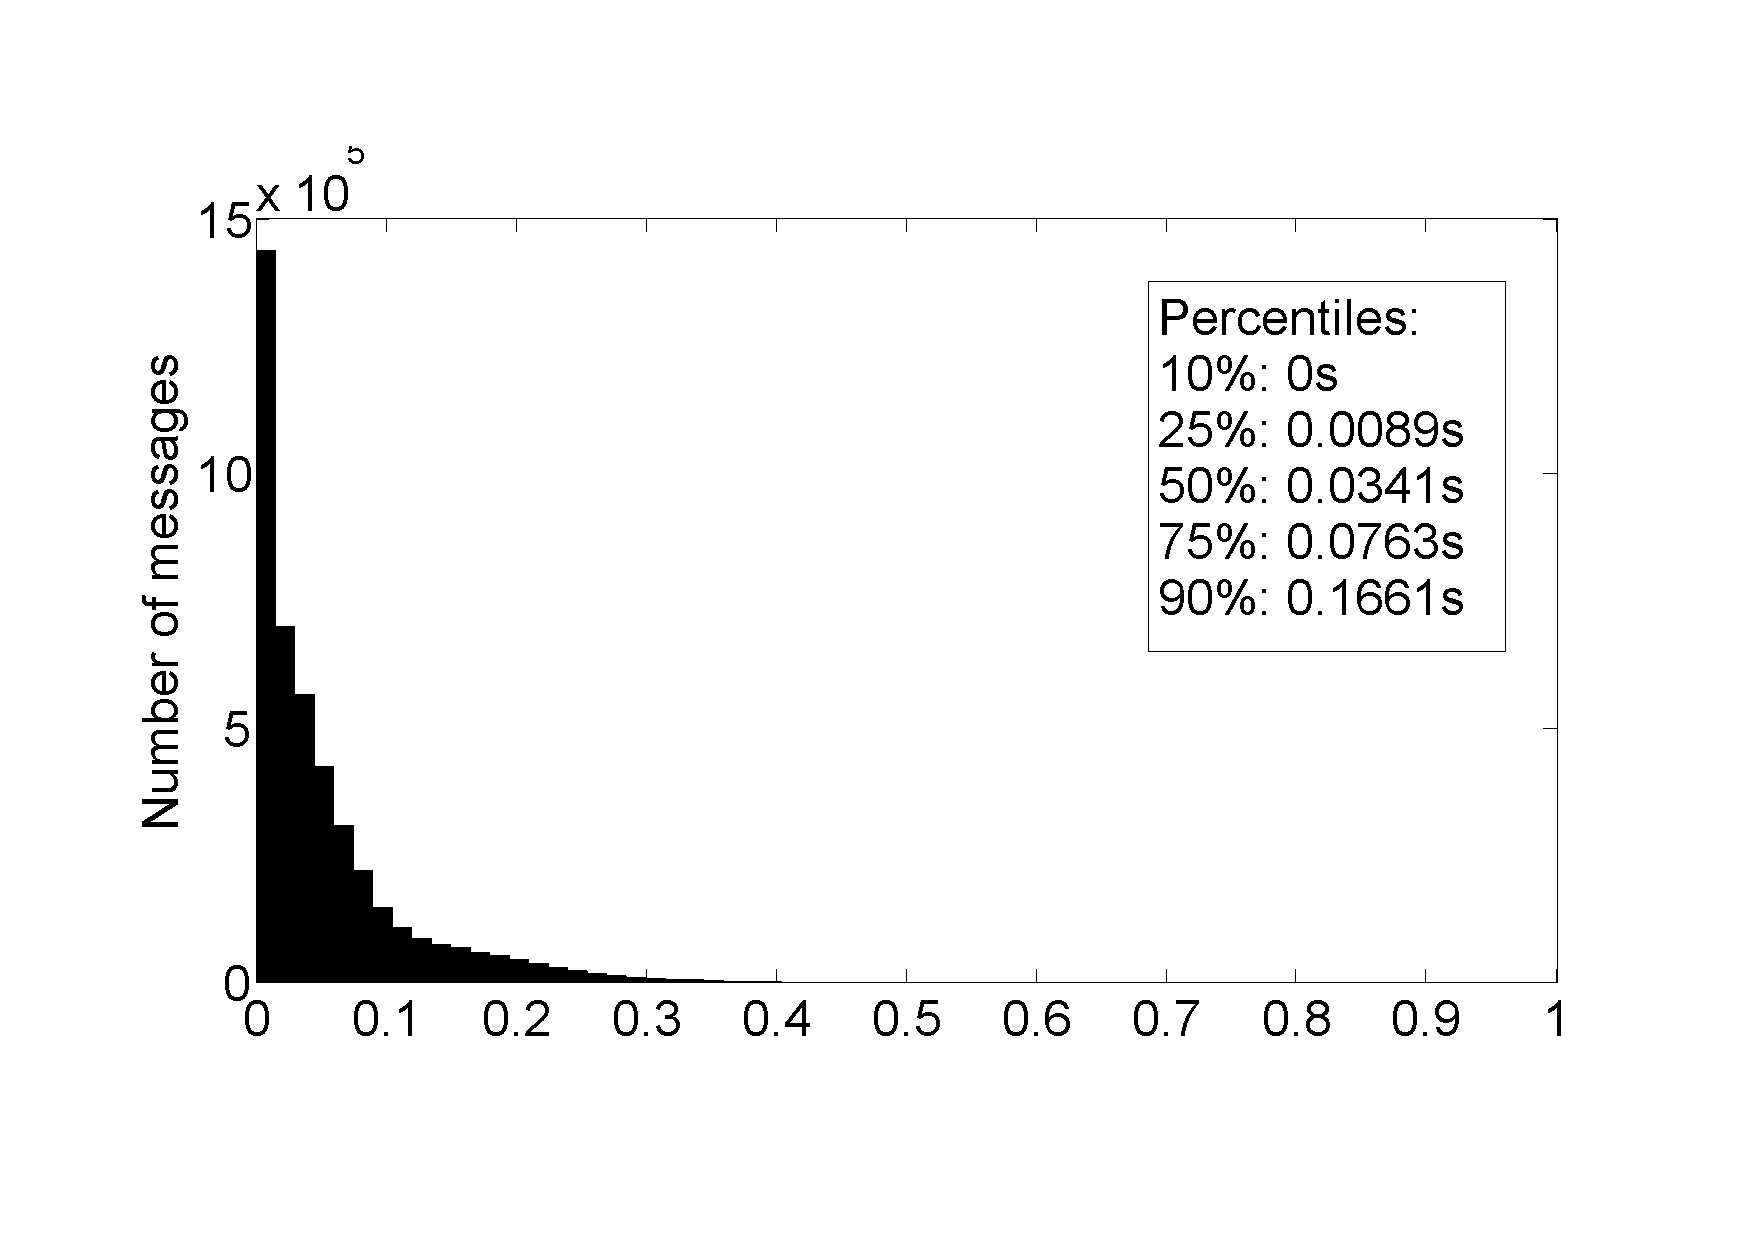
\includegraphics[clip=true, viewport=20mm 30mm 265mm 180mm, width=\columnwidth]{overall_get_fp}
 \caption{Overall retrieval responsiveness for fast storage and parallel retrieval}
 \label{fig_overall_get_fp}
\end{figure}
%
Figure \ref{fig_overall_get_fp} shows the overall retrieval responsiveness for parallel retrieval and safe or fast storage. Overall parallel retrieval mirrors parallel group retrieval, since parallel retrieval is faster than overlay retrieval and the first response is the one sent from the lower Pithos layers to peer logic.

\subsection{Conclusion}

In this section some responsiveness distributions were shown. The first reason was to enable the reader to not only compare mean performance values, but also range and shape. Secondly, it enables the highlighting of various structures and characteristics of storage and retrieval as they relate to certain quantities or mechanisms in Pithos, for examples timeouts. Thirdly, the distributions assist in verifying the correct working of Pithos. Especially when comparing the overall performance to the underlying group and overlay performance. It shows that Pithos is indeed a hybrid of those two storage types, but also that it is selecting the best quantities of the two. What this means is that any overlay can be selected and Pithos should perform better than the overlay.

\section{Performance for various group probabilities}
\label{group_probability_results}

The design of Pithos makes use of user groups and distance-based storage on a group layer, as stated in Sections \ref{grouping_design} and \ref{distance_based_design}. To be able to verify the actual performance of Pithos, it is therefore required to investigate Pithos's performance for various group probabilities. In the final P2P MMVE architecture, because of distance-based storage, it is assumed that the percentage of in-group requests will be much higher than that of out-of-group requests. This assumption is based on the fact that with group-based distance-based storage, the objects that are frequently of interest to the user will be stored in that user's group.

\subsection{Experimental setup}

\begin{itemize}
\item Because the exact probability that an object request will be for a group object is not yet known, a sweep is done for various group probabilities (the probability that a request is for a in-group object) to investigate the effect of group probability on Pithos's performance.

\item The ``low'' overlay is used for overlay storage. The low overlay was used to give a wider range of results from group storage to overlay storage.

 \item Fast  group storage is used.

 \item Fast group retrieval is used.

 \item Six object replicas are stored.

 \item Nodes have mean lifetimes of 1800s.

 \item Objects have a TTL of 300s.
\end{itemize}

\subsection{Reliability}

\begin{figure}[htbp]
 \centering
 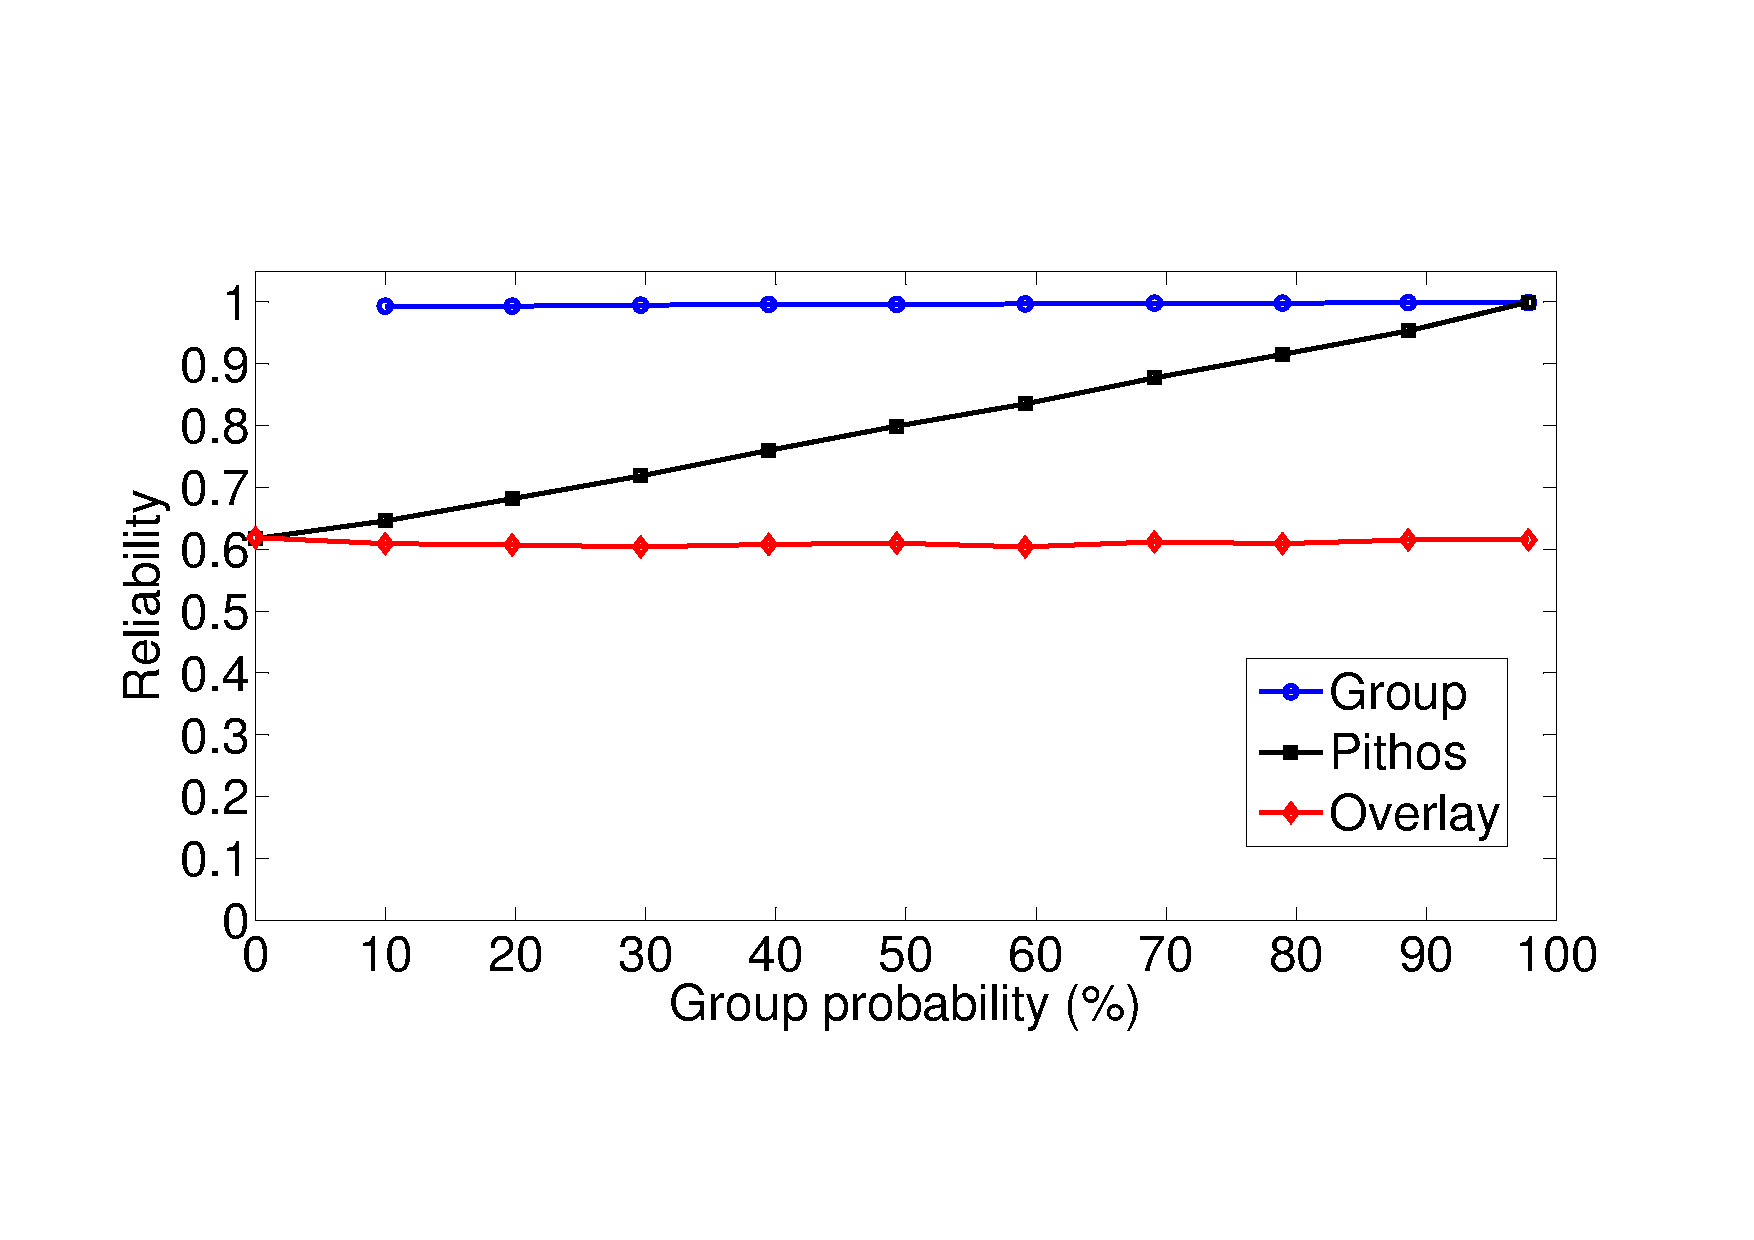
\includegraphics[clip=true, viewport=20mm 30mm 265mm 180mm, width=\columnwidth]{group_prob_rel}
 \caption{Reliability of Pithos, group storage and overlay storage for various group probabilities.}
 \label{fig_group_prob_rel}
\end{figure}
%
Figure \ref{fig_group_prob_rel} shows the effect group probability has on Pithos's overall reliability, compared with the underlying group storage and overlay storage reliabilities. The figure shows that the most reliable storage mechanism is group storage. It shows that group and overlay reliability are independent of the group percentage, which is as expected since the group storage and overlay storage modules are independent. Each request that is received from the higher layer (PithosTestApp) is relayed to both the DHT storage and group storage modules by the peer logic module.

When an object request is sent to group storage, the group storage module reports that there does not exist such a module in the group and the request is not handled. The only possible reply is then from the overly storage module. Figure \ref{fig_group_prob_rel} shows that the overall Pithos reliability is a linear combination of group storage and overlay storage, weighted by the group probability, or stated mathematically as:
%
\begin{equation}
R_{\textrm{Pithos}} = P_{\textrm{group}}R_{\textrm{group}} + (1-P_{\textrm{group}})R_{\textrm{overlay}},
\end{equation}
%
where $R_{\textrm{Pithos}}$ is the overall Pithos reliability, $R_{\textrm{group}}$ is the group reliability, $R_{\textrm{overlay}}$ and $P_{\textrm{group}}$ is the group probability.

This result shows that the reliability of Pithos varies linearly between overlay and group storage reliability as the group probability is varied. It should be noted that if a more reliable overlay was used, the medium or high configurations for example, the difference between group and overlay reliability is less. The low overlay configuration was just selected to better illustrate the linear relationship.

\subsection{Responsiveness}

\begin{figure}[htbp]
 \centering
 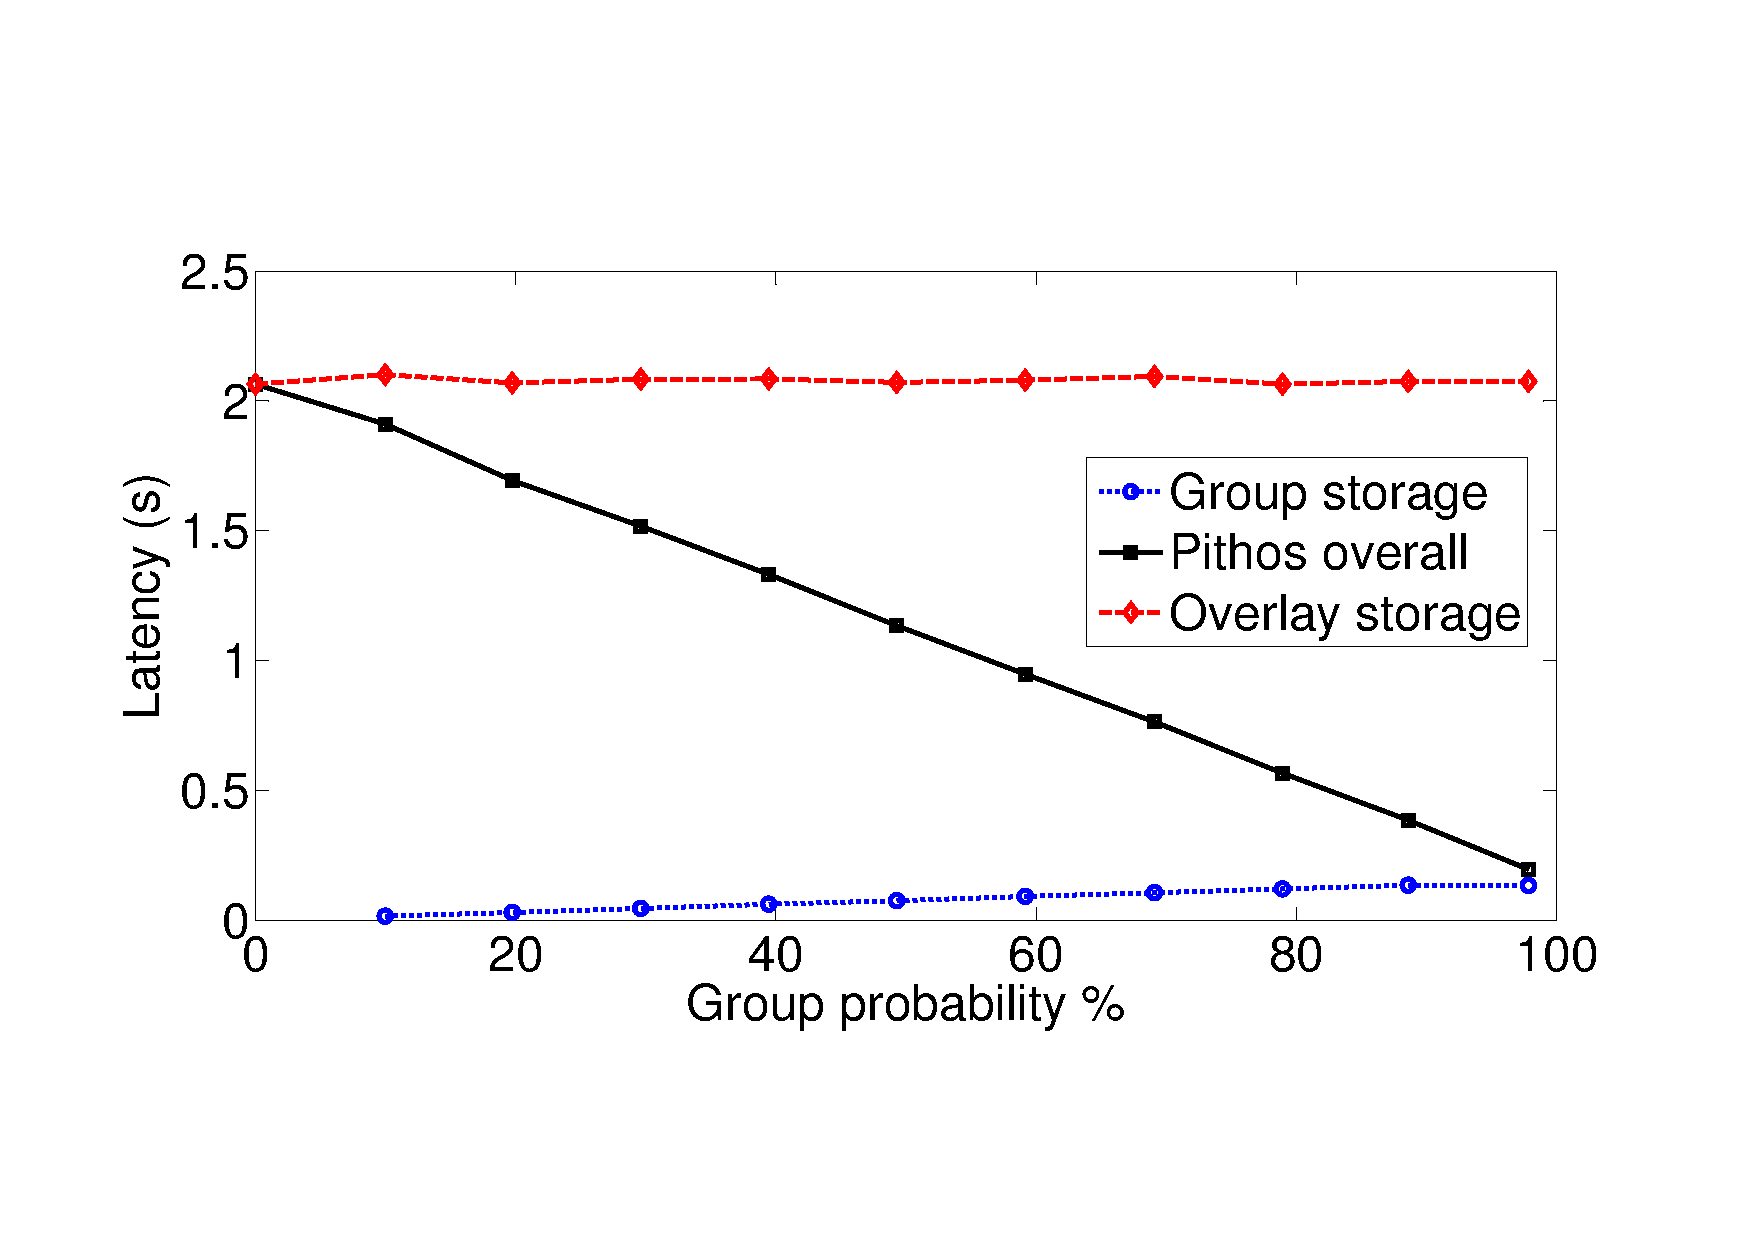
\includegraphics[clip=true, viewport=20mm 30mm 275mm 180mm, width=\columnwidth]{group_prob_resp}
 \caption{Responsiveness of Pithos, group storage and overlay storage for various group probabilities.}
 \label{fig_group_prob_resp}
\end{figure}
%
Figure \ref{fig_group_prob_resp} shows the responsiveness of Pithos compared with the underlying responsiveness of group and overlay storage. Take note that a lower value is preferred in this graph and that low latency is high responsiveness. As with the reliability, overall responsiveness is also shown to be a linear combination of group and overlay responsiveness.

An apparent anomaly is the group storage responsiveness that decreases with an increase in group probability. Recall that if a request is sent to group storage for an object not in the group, group storage immediately returns failure. The failure response is recorded as a response from group storage, even if this response is a failure.

The lower the group probability, the more failure responses are returned by group storage, which are returned instantly. It is these responses that decrease the mean group storage responsiveness for low group probabilities. When failure responses are ignored, group responsiveness remain constant at the value of 100\% group probability.

\subsection{Bandwidth}
\label{group_probability_bandwidth}

\begin{figure}[htbp]
 \centering
 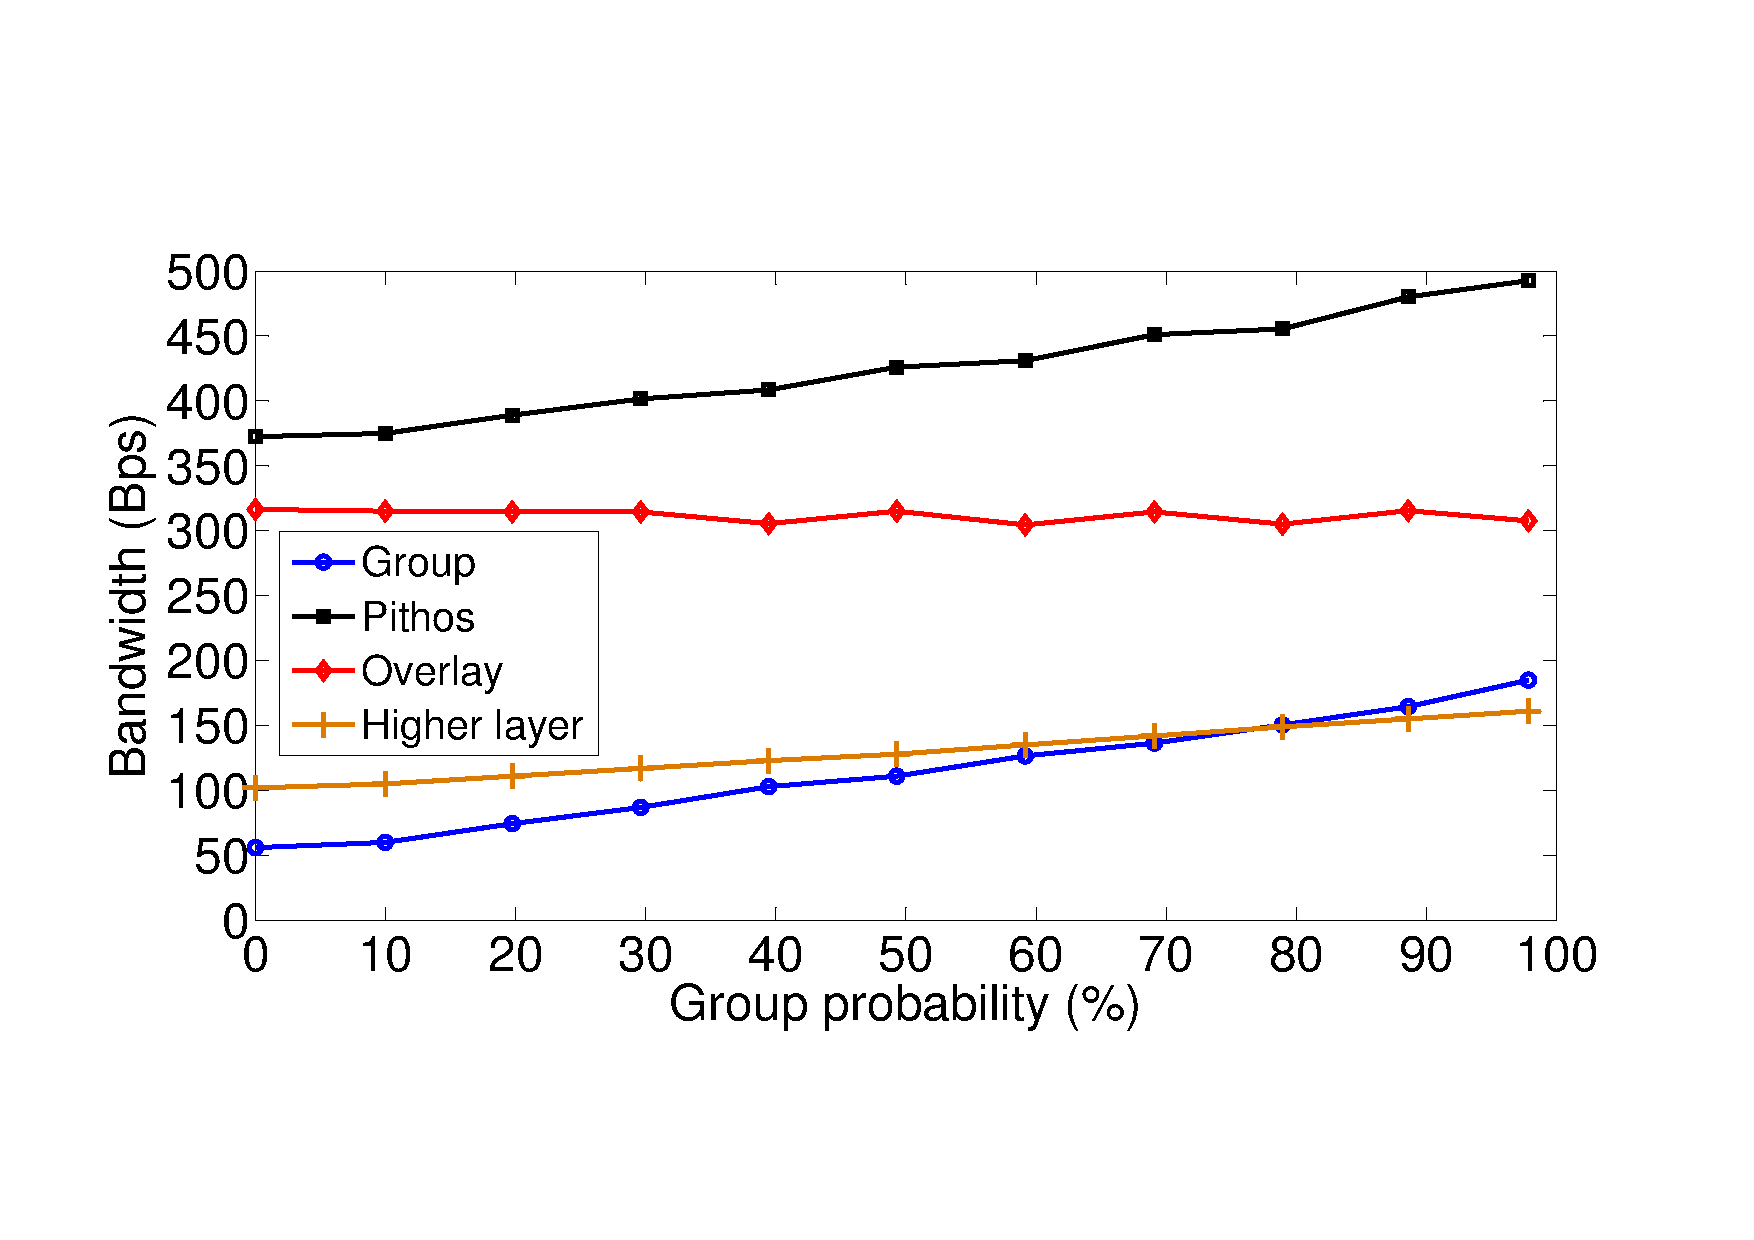
\includegraphics[clip=true, viewport=15mm 30mm 270mm 180mm, width=\columnwidth]{group_prob_bw}
 \caption{Bandwidth usage of Pithos, group storage and overlay storage for various group probabilities, as well as the bandwidth sent to, and received from Pithos.}
 \label{fig_group_prob_bw}
\end{figure}
%
Figure \ref{fig_group_prob_bw} shows the bandwidth requirements of Pithos in bytes per second (Bps). Pithos, group and overlay bandwidths show the mean of the inbound and outbound bandwidth. This was done, because the two values are similar and to make the graph more readable. Figure \ref{fig_group_prob_bw} also shows the underlying bandwidth requirements of group storage and overlay storage. To determine the actual overhead that Pithos requires, the graph also shows the amount of data that is sent to, and received from, Pithos, from and to the higher layer (PithosTestApp).

Figure \ref{fig_group_prob_bw} shows that overlay storage bandwidth remains constant, but that group storage bandwidth increases. Overlay storage remains constant, because no matter what the group probability is, the overlay storage is always queried for a data item and a data item is returned with the same probability (based on the reliability). Group storage, on the other hand, only returns data if the object exists within the group. Higher group probability means that more objects are requested from within the group, which means that group probability will return more objects and thereby use more data.

As shown, the overall Pithos bandwidth the the sum of the bandwidth required by group and overlay storage.

The data sent to Pithos is less than the data received from Pithos, because more retrieval requests are performed in the simulation than storage requests.

The graph shows that Pithos overhead is approximately 76\% of data in the network, where the majority of overhead is contributed by overlay storage.

\subsection{Conclusion}

This section reviews the performance of Pithos for various group probabilities and also shows the interaction between overlay and group storage in terms of reliability, responsiveness and bandwidth.

All all sections, what was seen was that for a low group probability, the characteristics of overlay storage are dominant and for high group probability, the characteristics of group storage are dominant. As previously stated, because of the distance-based storage design, high group probabilities are expected.

What was shown in this section is that overlay storage provides mediocre reliability for relatively high bandwidth requirements. This underpins the need for an overlay better suited to environments with network churn and improved lookup reliability. Before overlay efficiency can be improved, it is therefore important to create a grouping algorithm that has the highest possible group probability.

\section{Reliability under malicious nodes}
\label{malicious_results}

What remains to be shown is Pithos's resistance to malicious peers when safe retrieval is used, as described in Section \ref{pithos_retrieve}.

Each object in Pithos has a double value attribute that is set to a random value when an object is created for the simulation. The value of the object is stored in PithosTestApps's global object list. It should be noted that for simulation purposes, an object's size is not related to its content. An object's size is set using a random distribution and this is the value used to compute transmission bandwidth and latency.

Whenever a malicious node receives a retrieval request it replies with a modified version of the requested object. The object is modified by modifying the object value. An object is assigned a uniformly random value by a malicious node. Because of the way objects are altered, we implicitly assume that there exists no collusion in the network. When PithosTestApp receives a requested object, it checks that object against the global object list to determine whether the correct object was received. PithosTestApp then records Pithos's reliability.

Pithos selects the object that is the same in a majority of responses and sends it to the higher layer. If no object has a majority, a failure response is sent to the higher layer.

\subsection{Experimental setup}

\begin{itemize}
\item The percentage of users that are malicious is varied from 0.0 to 1.0 in steps of 0.125.

\item Fast group storage is used.

\item Fast and safe group retrieval are compared.

\item Six object replicas are stored.

\item For the safe retrieval case, six objects are retrieved.

\item A comparison of safe retrieval is performed by first retrieving four of the six stored replicas and then retrieving six.

\item Node lifetimes are set to 1800s mean.

\item Object TTL is set to 300s.
\end{itemize}

\subsection{Results}
\begin{figure}[htbp]
 \centering
 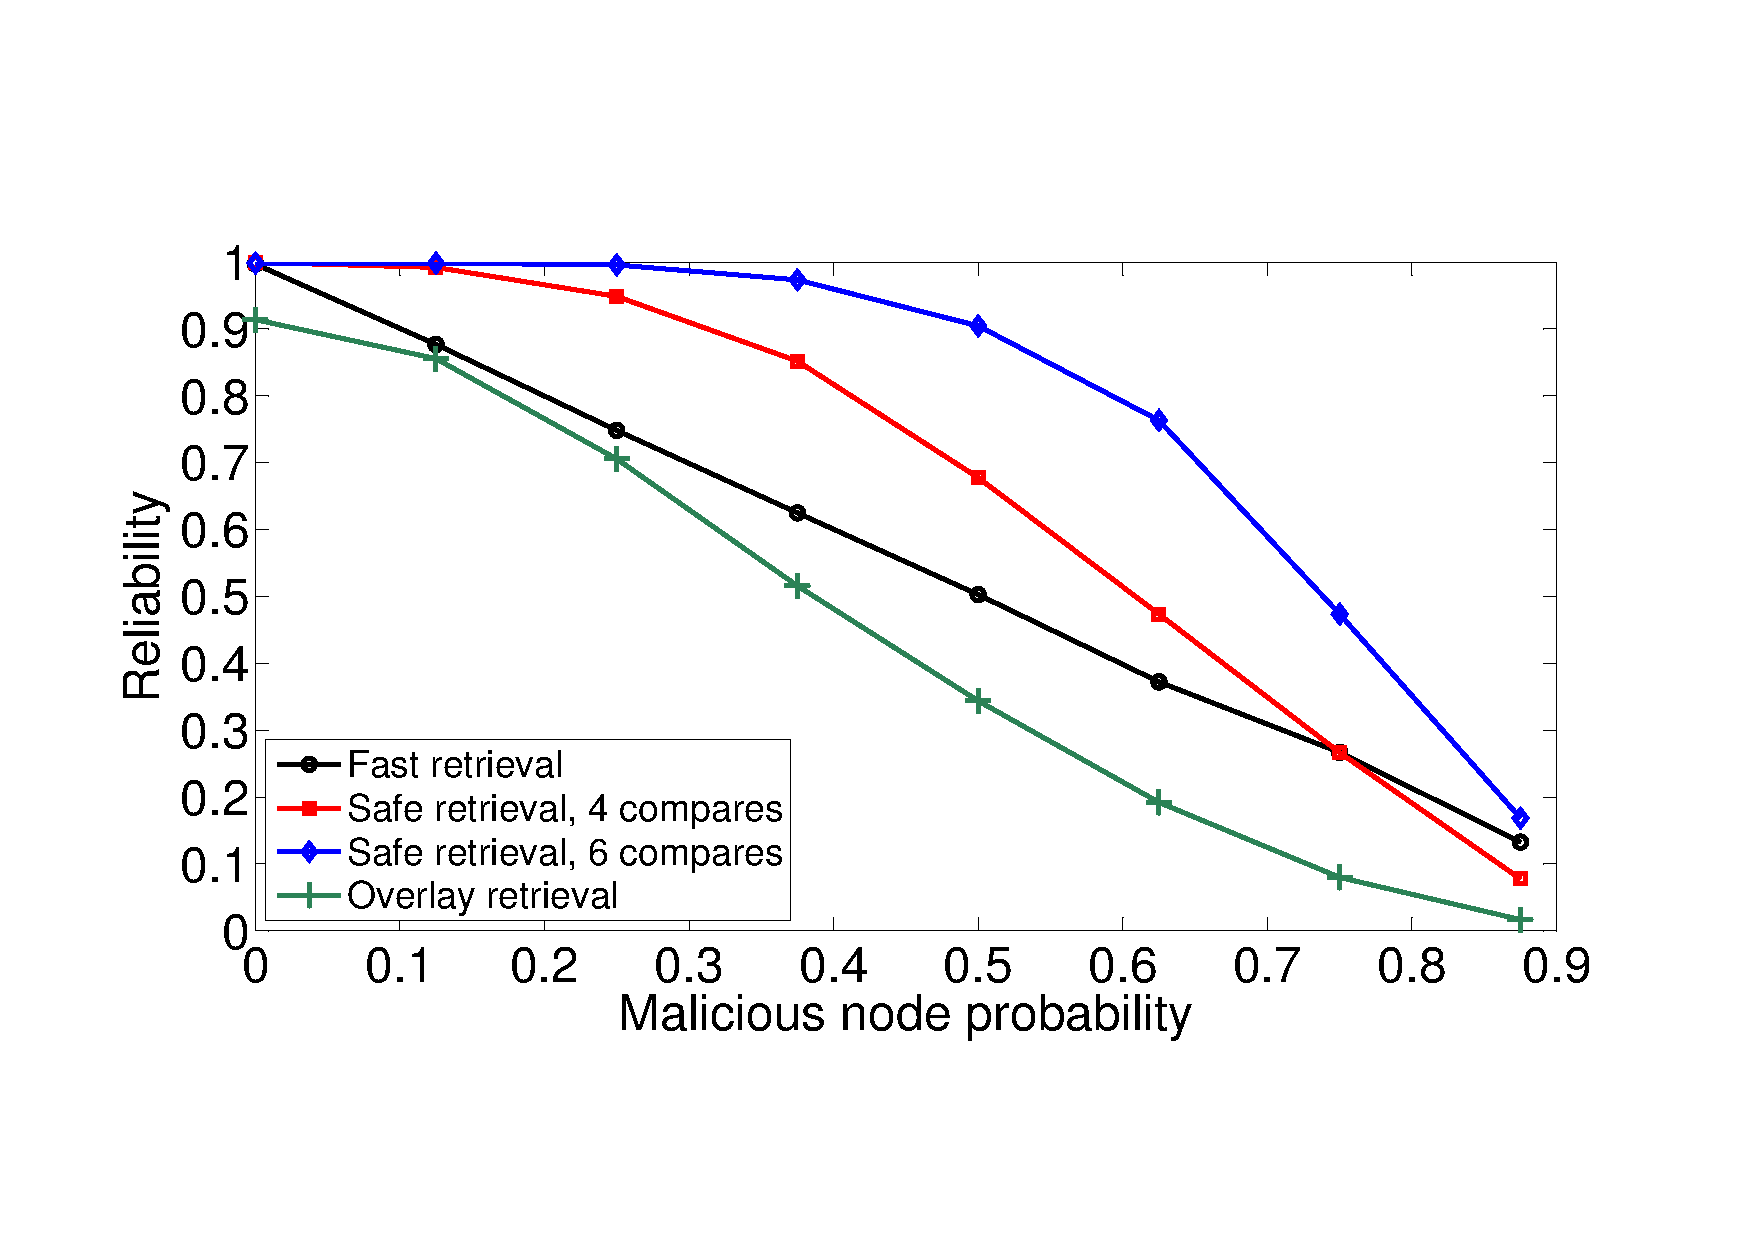
\includegraphics[clip=true, viewport=20mm 30mm 270mm 175mm, width=\columnwidth]{malicious_nodes_rel}
 \caption{Reliability of various Pithos retrieval schemes for varying factors of malicious node probability.}
 \label{fig_malicious_nodes_rel}
\end{figure}
%
Figure \ref{fig_malicious_nodes_rel} shows Pithos's reliability as a function of the percentage of malicious users in the network for both the fast retrieval and safe retrieval schemes. The fast retrieval reliability is almost the same as the malicious user percentage. System reliability for fast retrieval is the product of the malicious user factor and the system reliability under no malicious users.

The reason for this direct relationship is because the probability of an object retrieval being corrupted in the network is equal to the probability of a peer being malicious, since a malicious peer corrupts all objects returned and a non-malicious peer corrupts none of the objects returned. The overall probability is then the probability that an object retrieval would have succeeded if no malicious nodes were present, multiplied by the probability of nodes being malicious.

Figure \ref{fig_malicious_nodes_rel} also shows the improvement received from using safe retrieval. The curve shows that safe retrieval provides greater benefit for smaller factors of malicious nodes. As soon as the majority of objects are corrupted, object reliability drops significantly.

The figure also shows improved reliability, when more received objects are compared to select a majority. Retrieving more objects for comparison will, however, increase bandwidth requirements. Bandwidth increases in line with that shown in Section \ref{bandwidth_requirements}, because safe retrieval is parallel retrieval, but for an additional compare operation. It should be noted that more retrievals than compares may be performed to increase responsiveness at the cost of additional bandwidth.

An interesting situation arises, where safe retrieval reliability drops below fast retrieval reliability. When a majority can no longer be identified by safe retrieval, a failure response is sent up. This is as opposed to fast retrieval that sends any object received. It is possible the the object that was selected by fast storage was not maliciously altered, but also not in the majority. In this scenario, fast retrieval will sometimes send objects to the higher layer that were correct, where safe storage just responded with failure, because it couldn't be sure. Because in practice, the higher layer will not know whether an object is corrupted or not, it seemed more prudent to only send objects to the higher layer where Pithos was reasonably sure the object was unaltered.

Figure \ref{fig_malicious_nodes_rel} also shows the performance of overlay storage under the presence of malicious nodes if no security mechanisms are implemented in overlay storage. The performance degrades as the percentage of malicious users increase. The performance is also worse than the overall Pithos performance.  It should be noted that the overall Pithos performance is not influenced by Overlay storage in this graph, since 100\% group probability is used. For lower percentages of group probability, the linear relationship between group and overlay storage, explored in Section \ref{group_probability_results} exists.

\subsection{Conclusion}

The section shows that Pithos's safe retrieval mechanism can be used to increase reliability under malicious users at the cost of responsiveness and bandwidth. With malicious users usually present in a virtual world, this cost is always acceptable. During the lifetime of the virtual world, it is important to monitor that malicious user percentage, to determine how parameters, such as number of retrieve requests and number of compares, should be adjusted to combat the threat while minimising bandwidth and maximising responsiveness.

In practice, a low malicious node factor is expected, since it is assumed that cheaters are in the minority. If the virtual world has a majority of cheaters, it will most likely not be sustainable.

\section{Object distribution (fairness)}

One of the key reasons objects are distributed amongst groups is to achieve storage fairness. As described in Section \ref{fairness_requirement}, fairness is required to ensure that all peers contribute equally to the P2P network.

\begin{figure}[htbp]
 \centering
 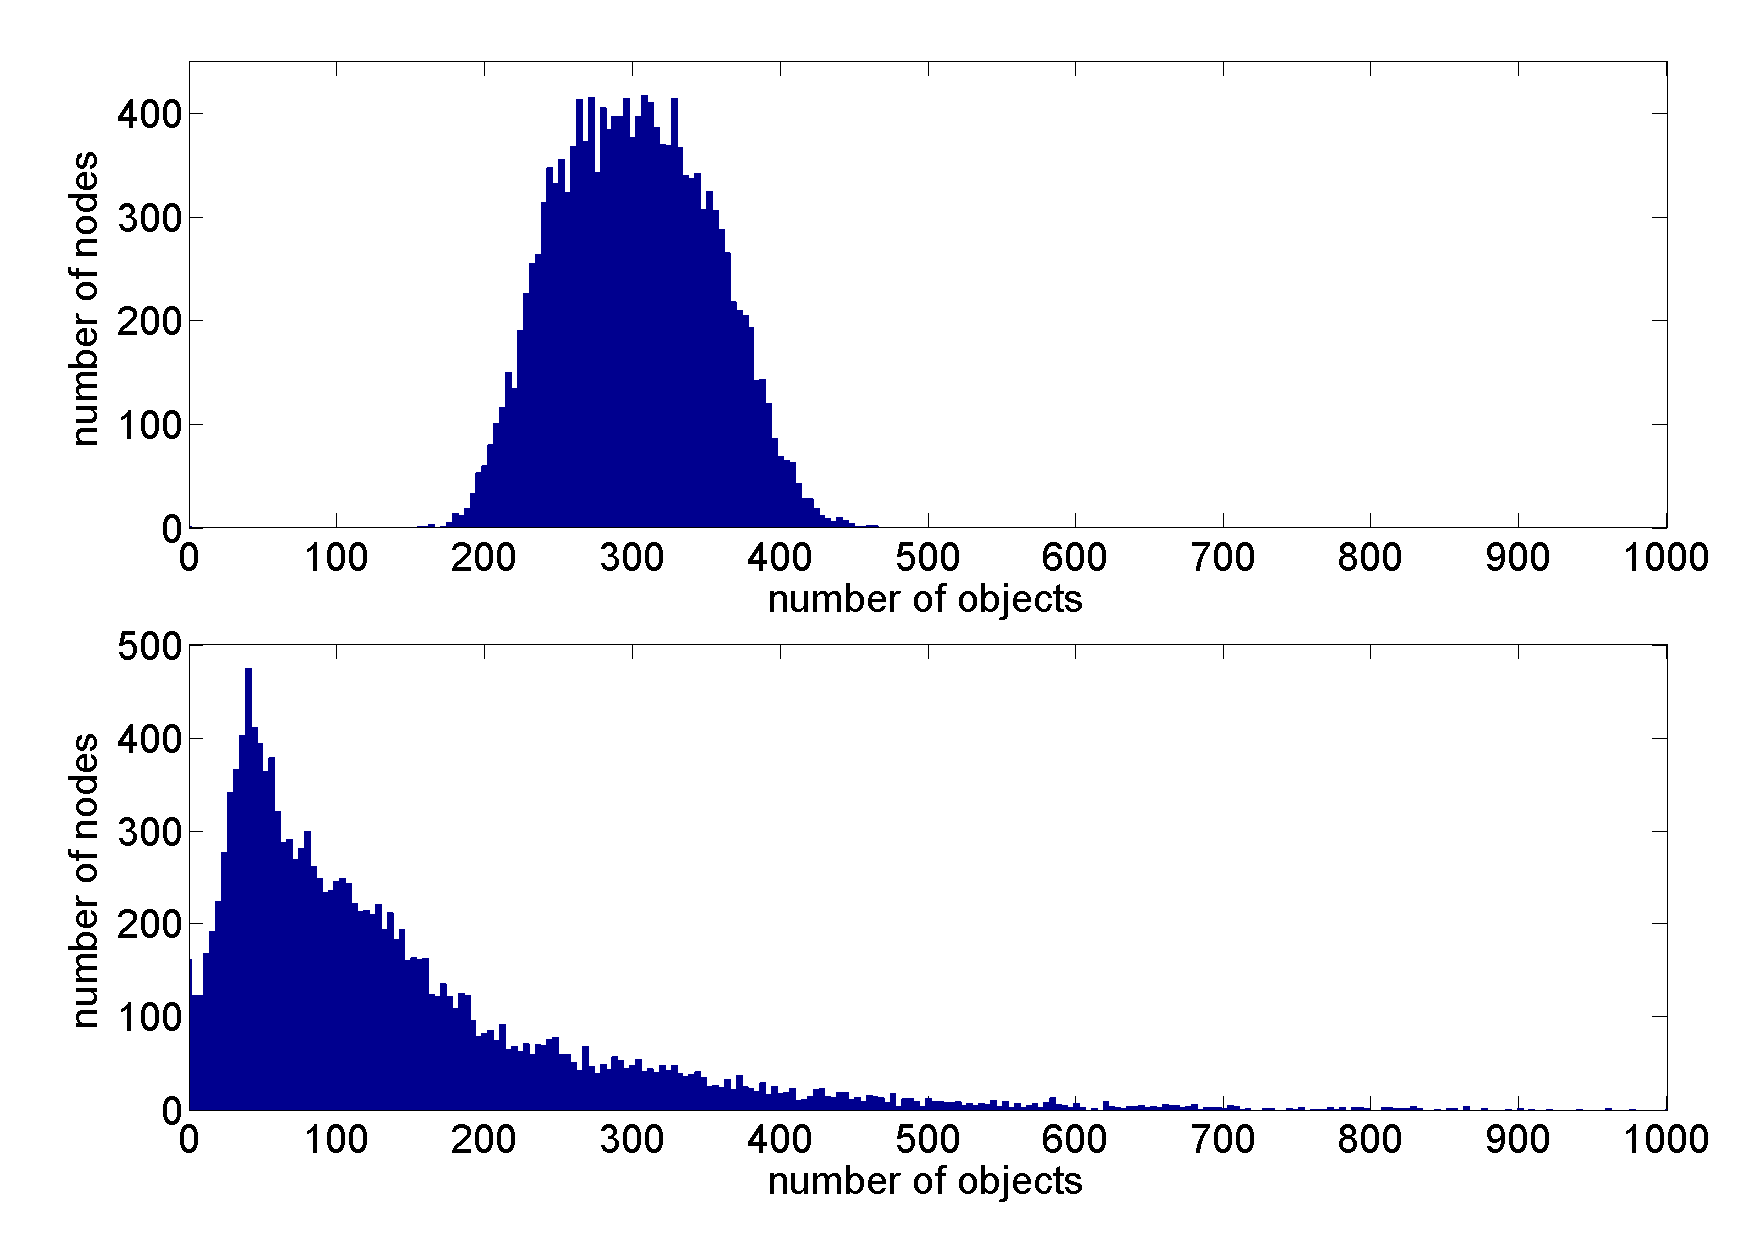
\includegraphics[clip=true, viewport=1cm 0.5cm 28.5cm 20cm, width=\columnwidth]{RootRepOverlayObjects}
 \caption{Top: Distribution showing the number of peers that store a certain number of group objects. Bottom: Distribution showing the number of peers that store a certain number of overlay objects.}
 \label{fig_group_overlay_objects}
\end{figure}
%
To evaluate the fairness, we evaluate the standard deviation of the number of objects stored per peer. Figure \ref{fig_group_overlay_objects} (top) shows the distribution of group objects over nodes in the network. The figure shows how many nodes store how many objects. The distribution has a mean and standard deviation of 302 and 51 objects per node respectively.

Figure \ref{fig_group_overlay_objects} (bottom) shows the distribution of overlay objects in Pithos with a mean and standard deviation of 153 and 189 objects per node respectively. Comparing the standard deviations of group storage to overlay storage, it appears that group storage is fairer than overlay storage.

\begin{figure}[htbp]
 \centering
 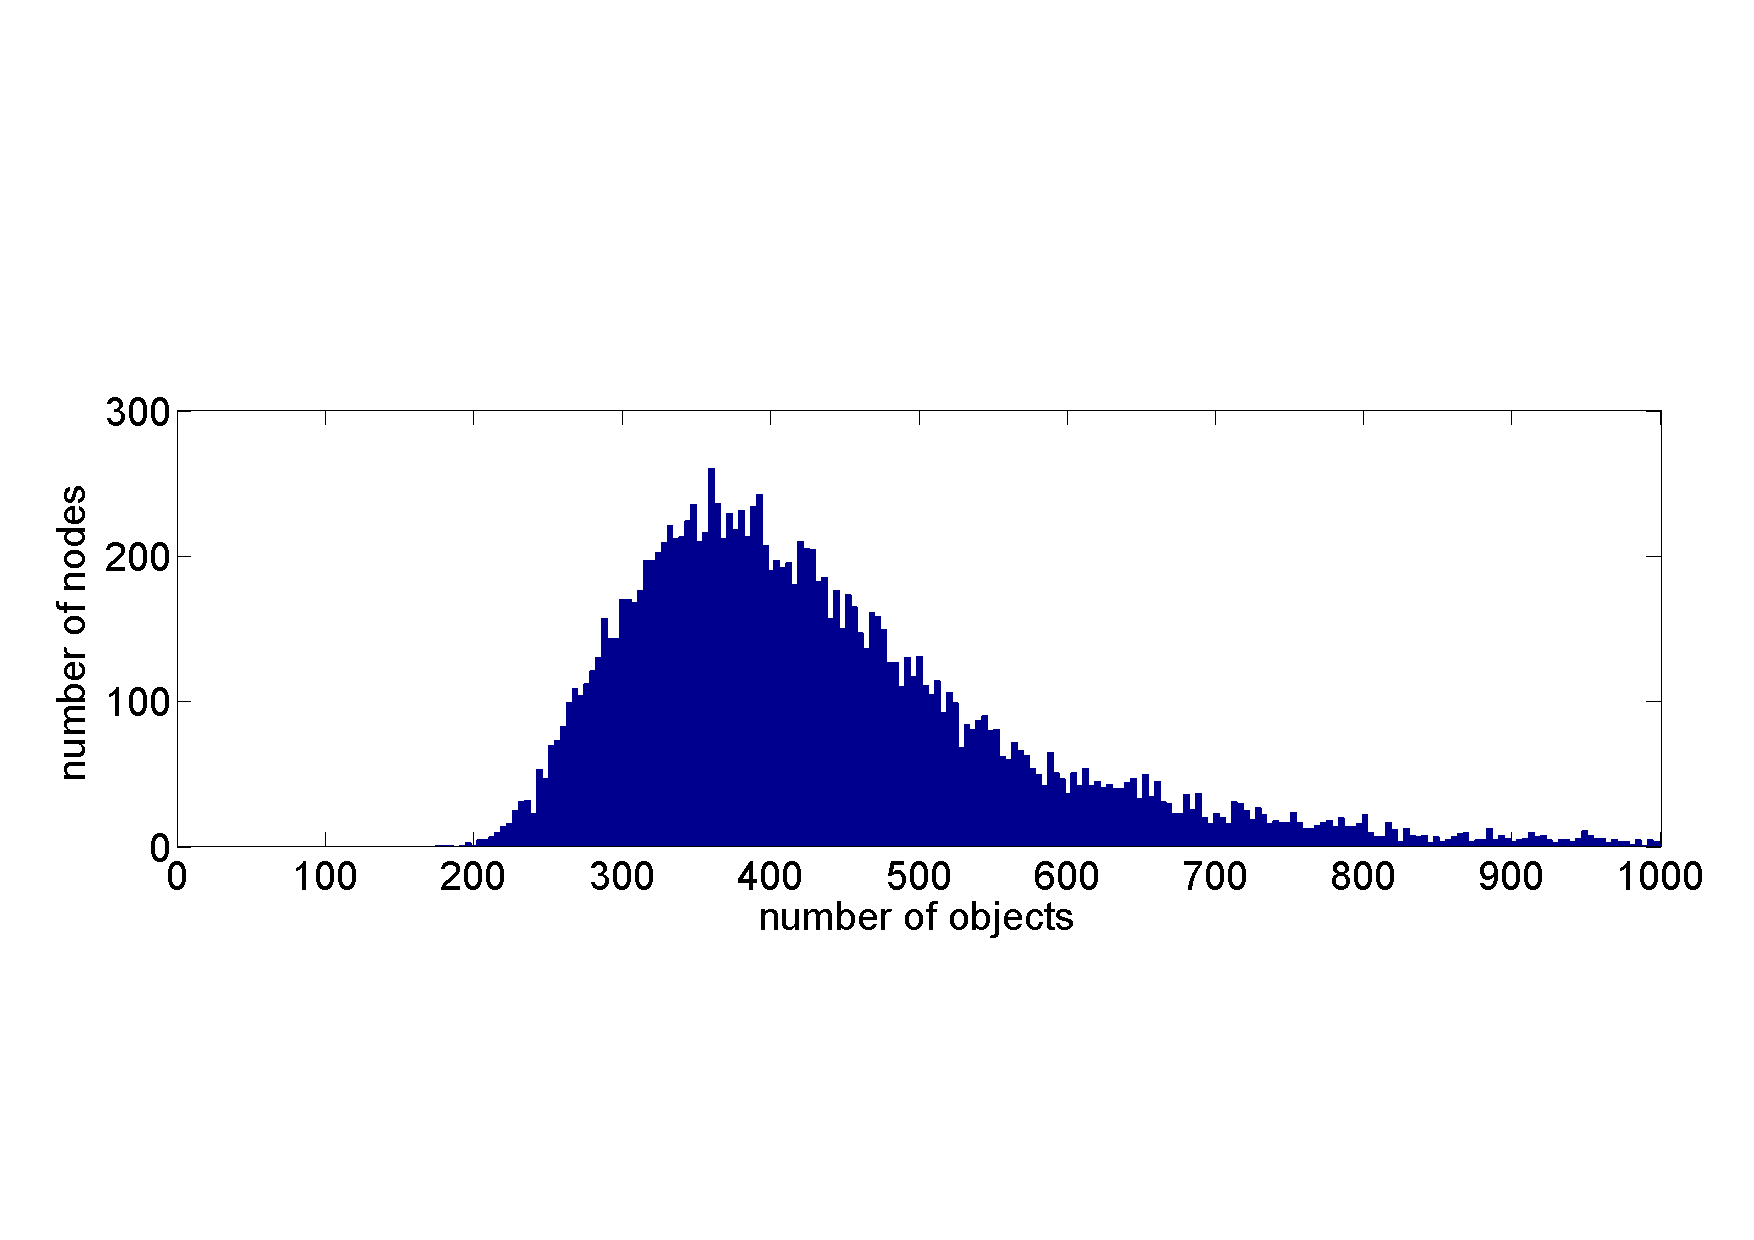
\includegraphics[clip=true, viewport=1cm 5cm 29cm 14.5cm, width=\columnwidth]{Objects}
 \caption{Combined object number distribution}
 \label{fig_objects}
\end{figure}
%
Figure \ref{fig_objects} shows the combined object distribution of Pithos, with a mean and standard deviation of 453 and 200 objects per node respectively. This shows that the fairness of Pithos is currently dominated by the fairness of the overlay and that Pithos is as fair as overlay storage.

What should be concluded from this section is that there does no exist a minority of peers in Pithos that store the majority of the data. All peers are required to contribute to the P2P network.

\section{Performance under object repair}
\label{repair_results}

Object replicas inserted into Pithos will all eventually disappear due to network churn. The rate at which replicas are removed from the network can be reduced by employing object repair. This enables Pithos to trade storage space for network bandwidth, by using fewer replicas with a higher repair rate. Network bandwidth can also be saved by having more replicas and a lower repair rate.

The effect of node replicas on the reliability and bandwidth efficiency of Pithos will be explored in this section. Reliability is tightly coupled to the lifetime of nodes, since nodes that live longer will store objects longer, meaning objects stored on nodes with longer expected lifetimes will have longer expected lifetimes. The main reason for being unable to retrieve an object from Pithos is because a peer has left the network. It is, therefore, expected that if nodes life longer the system reliability increases.

\section{Scalability}

As identified in Section \ref{scalability_req}, a key requirement of P2P MMVEs is that they should be scalable. It was argued that scalability is achieved when all other requirements are met, for a large numbers of nodes. The results shown thus far have been for a \emph{sufficiently scalable} system of 2500 nodes.

To show the scalability of the Pithos design and implementation, Pithos is simulated for 10,000 peers and 400 super peer, four times more peers and super peers than previously simulated.

\subsection{Simulation setup}

The fast storage and fast retrieval setup was used, with the same configuration parameters as in Section \ref{store_retrieve_exp_setup}:
%
\begin{itemize}
\item Nodes lifetimes of 1800s,
\item 98.3\% group probability,
\item medium overlay configuration,
\item 300s object TTL and
\item no repair.
\end{itemize}


The 10,400 peer simulation setup was not shown during the previous sections, because of the resources required to complete it. The simulation requires 19 hours of run time and 14 GB of RAM on an Intel Core i7, 3 GHz, quad core processor. A simulation on this scale would not have been possible using anything other than Oversim's simple underlay. The efficiency of the C++ language also provides great gains in terms of both processer and memory efficiency.

Although lengthy, a 19 hour simulation time is still a feasible time to performs simulations in.

\subsection{Results}

For both cases, the data from the higher layer was still measured as 4 Bps sent to Pithos and 157 Bps received from Pithos.

\begin{table}[htbp]
\centering
\begin{tabular}{|c|c|c|c|c|}
\hline
Number of peers & Module & Reliability & Responsiveness (s)  & Bandwidth \\
\hline
2600            & Overall&  0.9970     &   0.192             & 1370/1380 \\
2600            & Group  &  0.9775     &   0.134             & 187/183   \\
2600            & Overlay&  0.9140     &   1.760             & 1183/1197 \\
10,400          & Overall&  0.9971     &   0.191             & 1647/1657 \\
10,400          & Group  &  0.9819     &   0.134             & 180/177   \\
10,400          & Overlay&  0.9006     &   1.960             & 1467/1480 \\
\hline
\end{tabular}
\caption{Responsiveness and reliability of fast and parallel retrieval for safe and fast storage.}
\label{tab_pithos_scalability_results}
\end{table}
%
Table \ref{tab_pithos_scalability_results} shows the scalability of Pithos for large numbers of peers. Comparing group storage, it is evident that the reliability and responsiveness of the 2600 peer case is the same as that of the 10,400 peer case. Also of note is that group storage requires no more bandwidth for larger numbers of nodes. The results show group storage to be very scalable.

Overlay storage, however, fares worse both in responsiveness as well as required bandwidth.

Overall, Pithos is as reliable and responsive for 2600 peers as it is for 10,400 peers, with the exception that it uses somewhat more bandwidth, which has been shown to be as a consequence of the overlay storage not scaling as well as group storage.

This section shows that Pithos is scalable for large numbers of nodes in terms of responsiveness, reliability as well as bandwidth requirements.

\subsection{Experimental setup}

\begin{itemize}
\item Node lifetimes are varied from 100s to 1800s in irregular steps that are closer together for lower peer lifetimes.

\item Fast group storage is used.

\item Fast group retrieval is used for the no repair, leaving repair and periodic repair cases.

\item Parallel retrieve with no repair is also compared.

\item Six object replicas are stored.

\item Object TTL is set to 1000s.
\end{itemize}

\subsection{Reliability}

\begin{figure}[htbp]
 \centering
 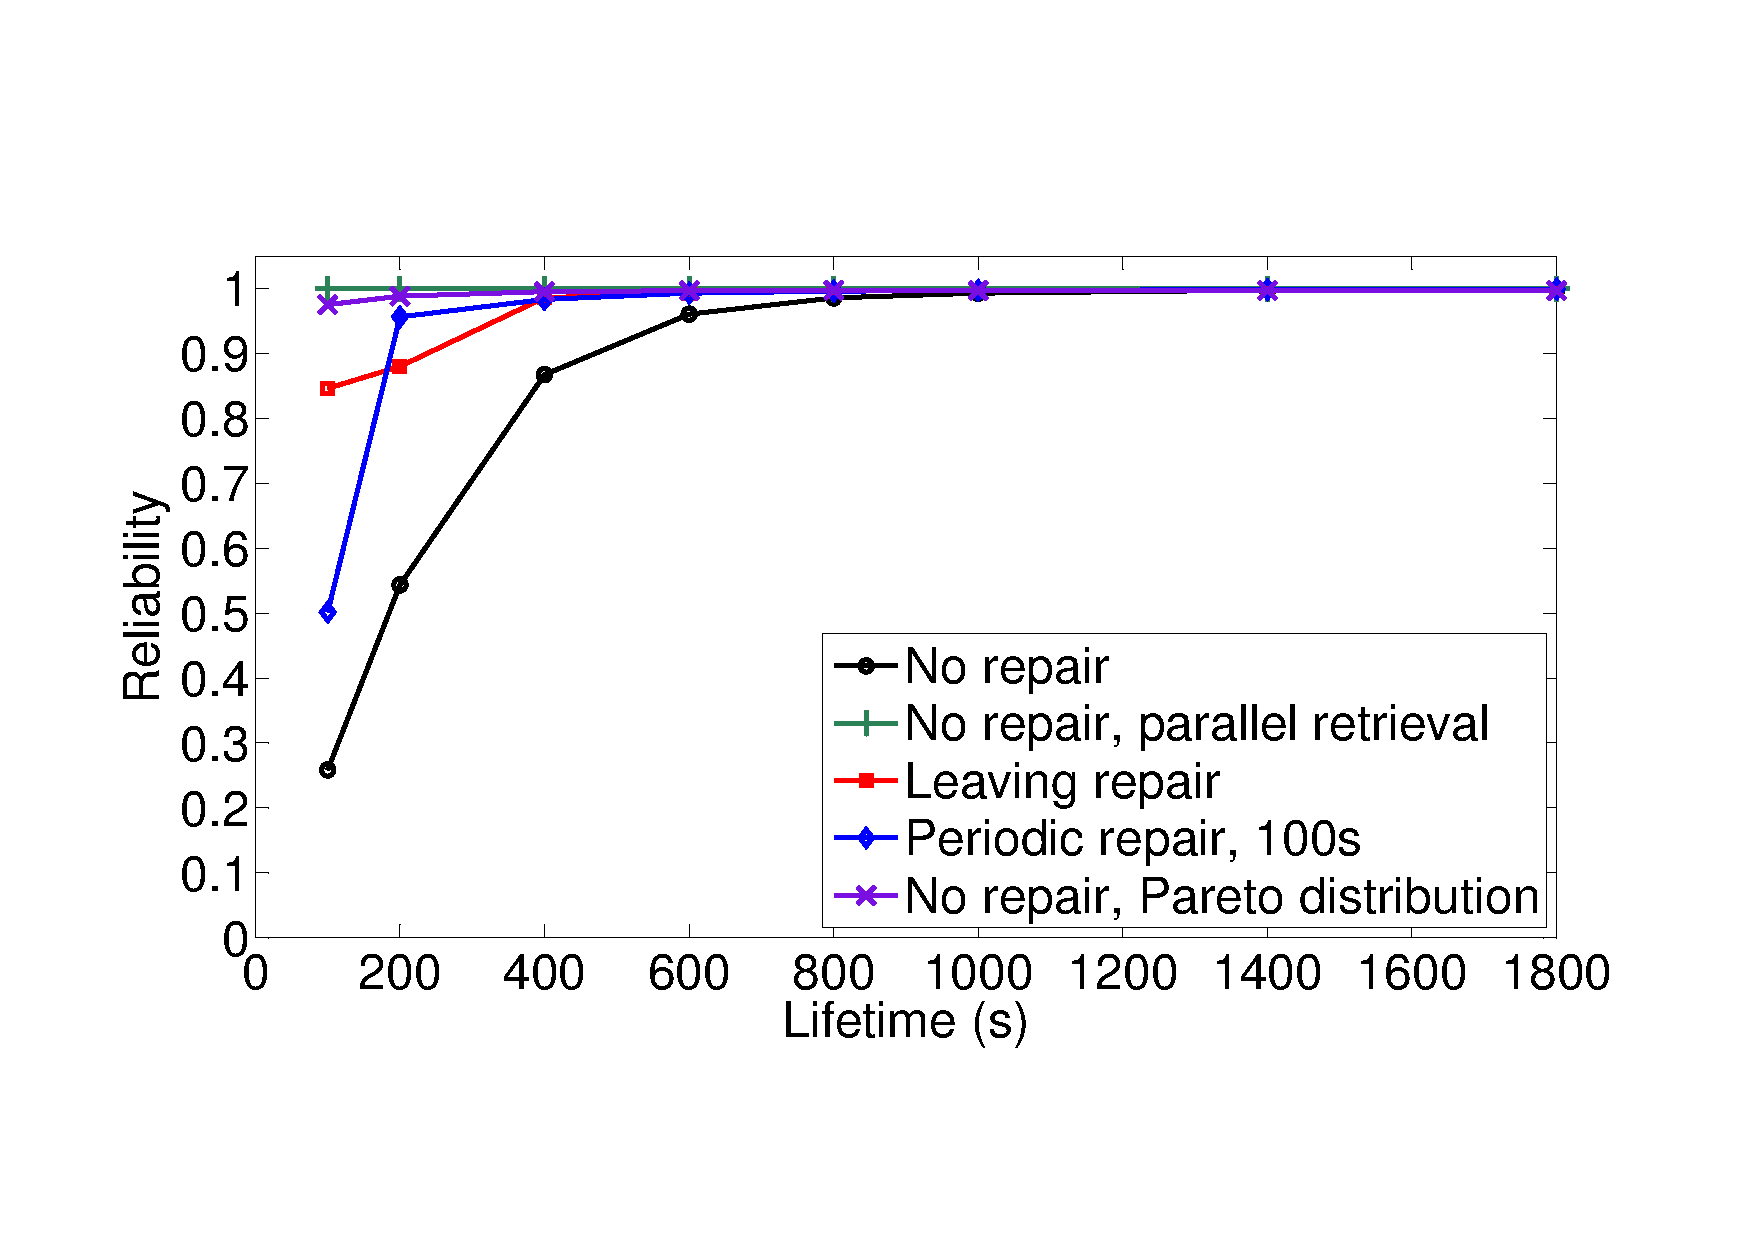
\includegraphics[clip=true, viewport=15mm 30mm 275mm 180mm, width=\columnwidth]{repair_rel}
 \caption{Reliability of Pithos for various node lifetimes, comparing no repair, no repair with parallel retrieval, leaving repair and periodic repair with 100s periods.}
 \label{fig_repair_rel}
\end{figure}
%
Figure \ref{fig_repair_rel} shows request reliability for various node lifetimes for no repair, no repair using parallel retrieve, leaving repair and periodic repair.

As expected, doing no repair does not cope well with short node lifetimes compared to an object TTL of 1000s. The object TTL is important when evaluating performance, since a network that requires objects to be stored for longer has to maintain the object replicas for a longer amount of time. When the expected node lifetime is equal to the object TTL at 1000s, the reliability of the system when not using repair is similar to the the system reliability when repair is used.

This observation is helpful when designing a P2P MMVE. Objects might be classified according to how long their should remain in the system. Objects that should only remain in the system for approximately the same amount of time as the expected user session time need not use repair mechanisms, if a sufficient number of replicas are used.

When node lifetimes are the same as the periodic repair interval, leaving repair copes better than periodic repair. The periodic repair mechanism might be adjusted to less than the minimum expected node lifetime in the system, but this will increase the load on the super peer, which has to perform the periodic checks. From the data is seems that leaving repair might be able to better handle a situation where node lifetimes have a high dynamic range, since the rate at which nodes leave the network is directly tied to how often leaving repair performs repairs.

Except for the case where the periodic repair timer is equal to the expected node lifetime, leaving and periodic repair appear to perform similarly in terms of reliability.

Parallel retrieval, employing no repair mechanism, is most reliable and consistently reliable for all node lifetimes.

\subsection{Bandwidth efficiency}

\begin{figure}[htbp]
 \centering
 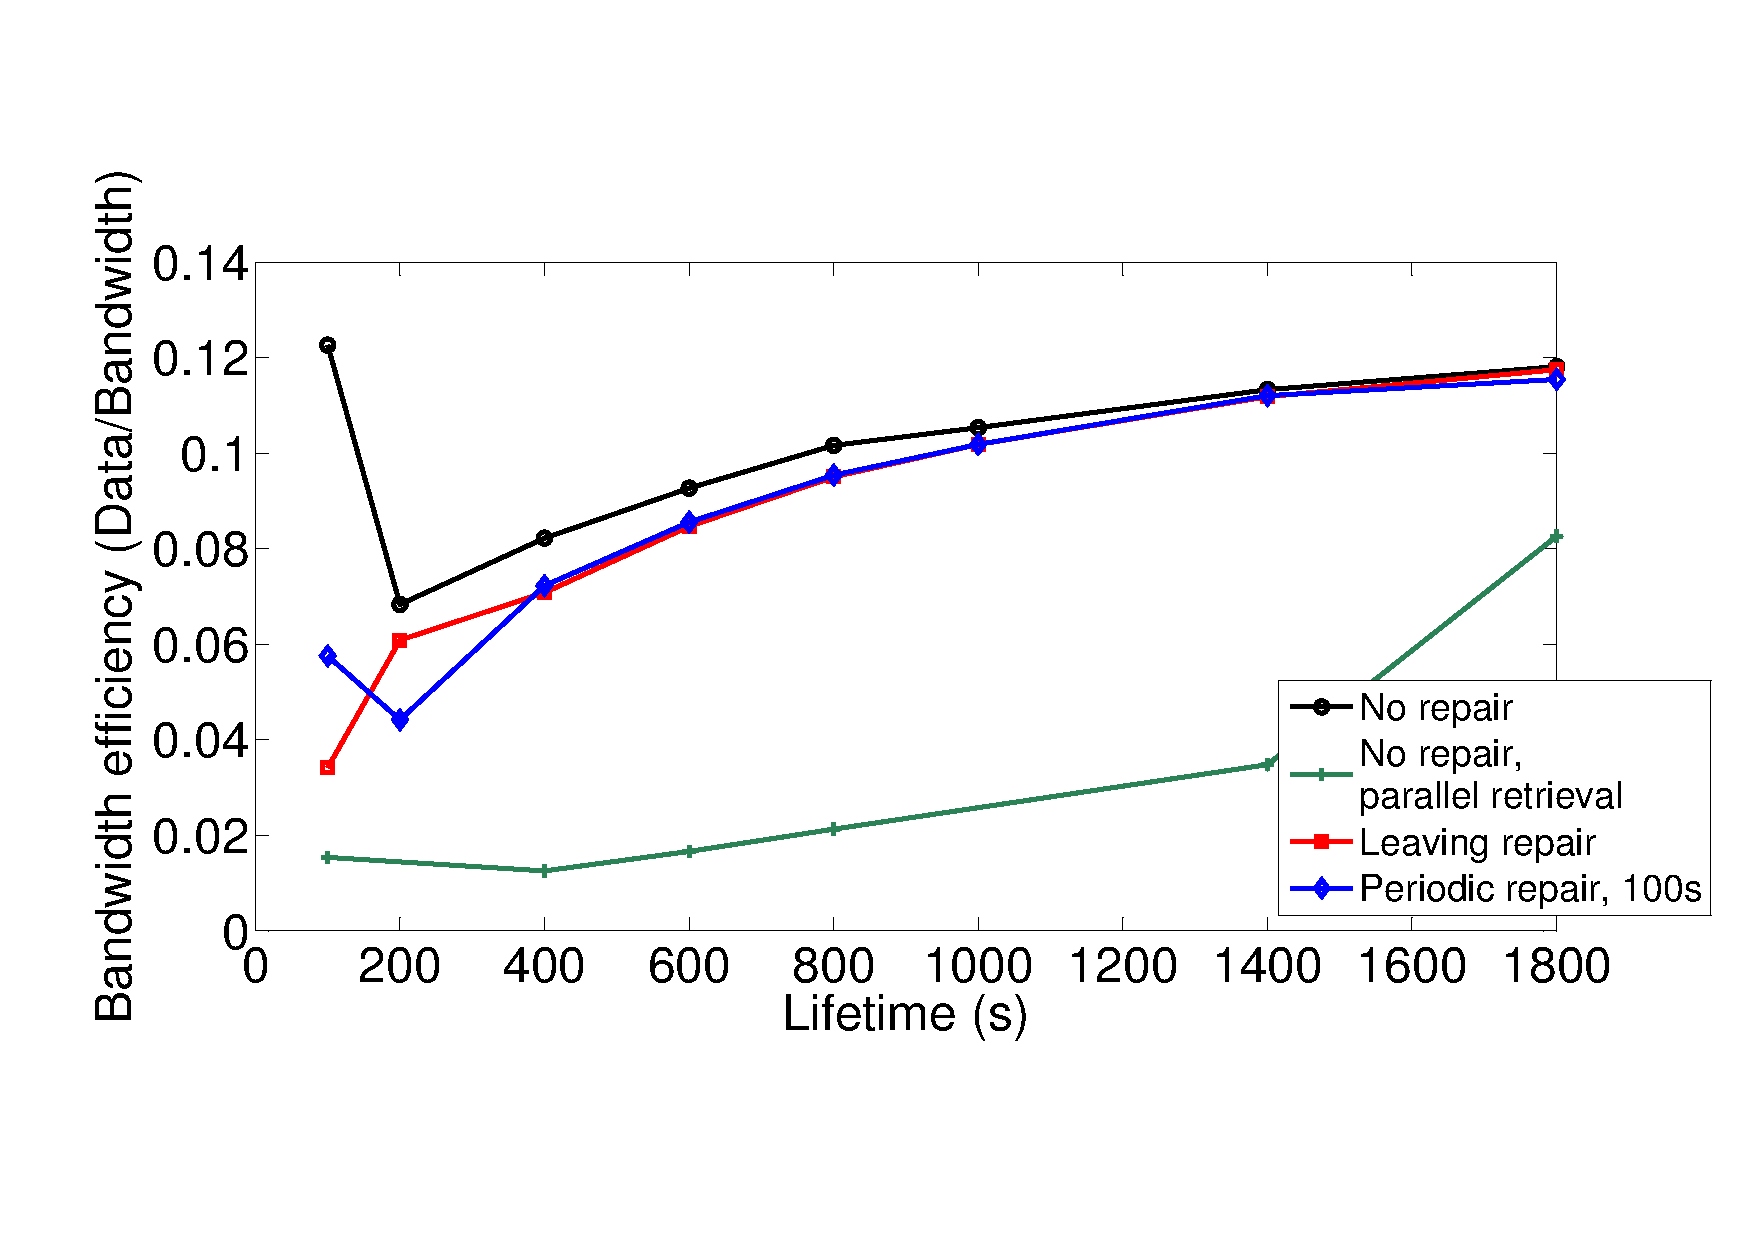
\includegraphics[clip=true, viewport=15mm 30mm 275mm 180mm, width=\columnwidth]{repair_bw_eff}
 \caption{Bandwidth efficiency of Pithos for various node lifetimes, comparing no repair, no repair with parallel retrieval, leaving repair and periodic repair with 100s periods.}
 \label{fig_repair_bw_eff}
\end{figure}
%
Figure \ref{fig_repair_bw_eff} compares the bandwidth efficiency of the various repair techniques. Bandwidth efficiency is defined to be the factor of usable data that would have been transferred to the higher layer, had the system been 100\% reliable, compared to the total bandwidth used by Pithos. 100\% reliability is used, otherwise bandwidth efficiency is also a function of reliability, since less data is transferred if fewer requests are successful. It should be noted that the largest part of Pithos's bandwidth usage is contributed by overlay storage, as shown in Sections \ref{overlay_results} and \ref{group_probability_bandwidth}.

Although parallel retrieval was shown to be the most reliable retrieval mechanisms for various node lifetimes, Figure \ref{fig_repair_bw_eff} shows that it is also the most bandwidth inefficient, with only between 1.5\% to 8\% usable data transferred. The bandwidth efficiency of leaving and periodic repair are similar for long peer lifetimes, compared to the periodic repair timer.

Bandwidth efficiency is monotonously increasing, because as peers remain in the network for longer periods of time, less bandwidth is required to repair missing replicas. Bandwidth efficiency also increases, since there is more usable data transferred when peers are alive for longer periods of time. Peers that live longer have less time to generate usable data. The increase in usable data for longer node lifetimes, than the object TTL does not lead to a significant increase in Pithos bandwidth.

Although doing no repair is less reliable, it is more bandwidth efficient, because no object repairs have to be performed.

\subsection{Conclusion}

The leaving and periodic repair mechanisms were found to posses similar reliability and bandwidth performances. It seemed that leaving repair does, however, cope better with dynamic node lifetimes. A periodic timer also has to be designed for specific network parameters, including expected node lifetime and object TTL. If, during the lifetime of the network, the parameters change, the system will not be able to dynamically adapt.

As expected, doing no repair is less reliable than doing repair, but uses less bandwidth. Parallel retrieval is highly reliable, but requires a large amount of bandwidth.

\section{Conclusion}

This section initially showed the storage and retrieval performance of Pithos, without taking into account group probability, object repair or malicious nodes. Fast storage was found to be sufficiently reliable for the large responsiveness gain it added. It was found that parallel storage are both more responsive and reliable than fast storage at the cost of additional bandwidth.

Overlay storage was found to be less reliable than initially thought, when taking into account its required bandwidth. Overlay storage is, however, the only way in which a peer may acquire data from outside of its group.

The responsiveness distributions for Pithos were also presented, along with a discussion of the results. The distributions verified the methods used to implement the store and retrieve mechanisms and also showed how the underlying group and overlay storage modules relate to the overall storage performance.

It was discussed that it is important to take group probability into account when evaluating Pithos performance. By varying the group probability, it was shown that the overall performance is a weighted average of the underlying group and overlay performances.

Tt was shown that all peers in Pithos are required to contribute storage space to the network.

The effect of repair was shown by evaluating Pithos for various repair methods with varying node lifetimes. It was found that repair significantly increases reliability when the expected node lifetimes are small, compared to the object TTL. Repair is not required, if node lifetimes are large, compared to the object TTL.

From the evaluation of object repair, it was found that there are many factors that influence how retrieval reliability. On a basic level, retrieval reliability is directly proportional to object lifetime. From the results shown, it was found that object lifetime is, therefore, related to node lifetimes, repair rates and object TTL.

It should be possible to design a storage system with predictable levels of reliability, to ensure correct functionality of the larger system that uses the storage system. It is, therefore, of benefit to be able to predict objects lifetimes in a distributed storage system. Of greater benefit is to be able to design a storage system to ensure required levels of expected object lifetimes. This is the focus of the next chapter. Predicting object lifetimes in finite network under churn.

\chapter{Modelling object lifetimes in finite networks under churn}
\label{chp:MODELLING}

%Test required

    %%%%%%%%%%%%%%%%%%%%%%%%%%%%%%%%%%%%%%%%%%%%%%%%%%%%%%%%%%%%%%%%%%%%%%%
\section{Background and related work}
\label{related_work}

To increase the time an object is available within the distributed storage system, two techniques are used: redundancy and repair. In storage systems using replication as redundancy technique, $R$ replicas of every object are stored. The number of required replicas $R$ is a design decision, the effect of which will be shown in Section \ref{results}. When all nodes containing an object's replicas have left the network, the object is no longer available. Periodic repair, which occurs at a rate of $\mu = 1/T_{\textrm{repair}}$, replaces all missing replicas.

This chapter mainly extends and improves upon the work by Wu, Tian and Ng \cite{replication_article}. The related work models three characteristics of distributed hash table (DHT) lookups under churn: expected lookup latency of various routing schemes, expected lookup overhead of various routing schemes and expected object lifetime. We focus on the object lifetime characteristic. Wu, Tian and Ng develop two models for object lifetime when exponentially distributed node lifetimes are assumed. One for the case without object repair and one for the case with object repair. Node residual lifetimes are used when calculating expected object lifetimes without repair. In this case object lifetimes are equal to the maximum residual lifetime of the nodes the objects were replicated on.

%What about Pareto lifetimes?

A continuous time Markov chain, shown in Figure \ref{fig_other_markov_chain}, is used to model the expected object lifetimes for the case with repair.
%
\begin{figure}[htbp]
 \centering
 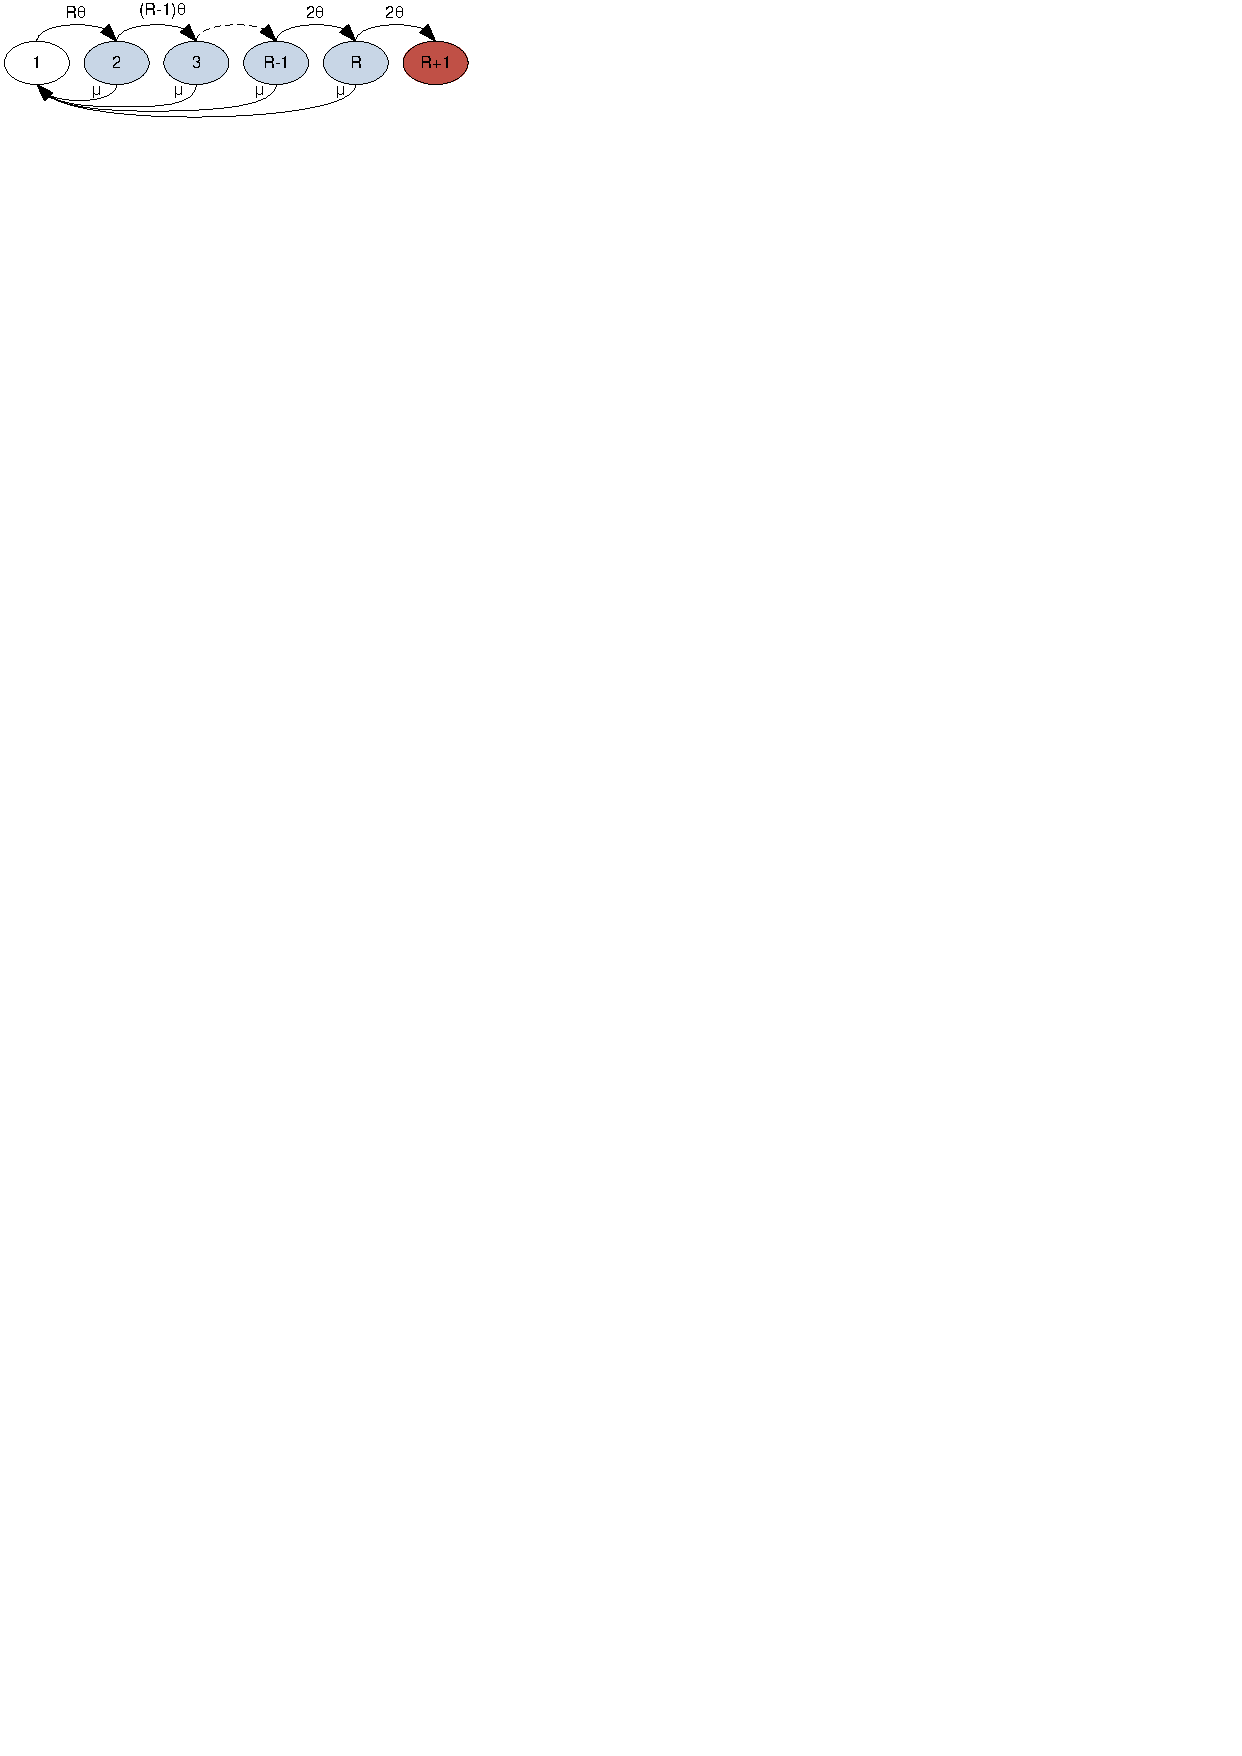
\includegraphics[clip=true, viewport=0.0cm 27.5cm 8.0cm 30.0cm, width=0.7\columnwidth]{inifinite_network_chain}
 \caption{Markov chain modeling object replica number for an infinite network size}
 \label{fig_other_markov_chain}
\end{figure}
%
The model has $R+1$ states and is in state $k$ when $R+1-k$ replicas are alive in the network. The system is, therefore, in state $1$ when all replicas are present and in state $R+1$ when no replicas are present. The authors assume that all objects are inserted into the network with $R$ replicas, i.e. enter the network in state 1. This initial state is colored white in Figure \ref{fig_other_markov_chain}. If the node departure rate under steady state is $\theta$ and there are $r$ replicas present in the network, the replica departure rate under steady state is $r\theta$. When all replicas are lost, the chain enters state $R+1$ (coloured dark) and is said to be ``absorbed''.

In this chapter, we improve on the work by Wu, Tian and Ng \cite{replication_article} in two ways: firstly, the model is extended to take into account a finite network size. The fact that there might not be sufficient nodes to replicate the data on when objects are stored or when the repair mechanism activates. Secondly, our model unifies the cases with and without repair, to produce a single model where the effects of both might be evaluated. When our model is used with larger average network sizes, expected object lifetimes converge to those shown in the work by Wu, Tian and Ng, using their two separate models.

Predicting object lifetimes in a distributed storage system is grounded in reliability engineering theory. When network size is ignored, it is similar to predicting the mean time to failure (MTTF) of a set of parallel components with repair. Chun et al. \cite{Chun:2006_replica_maintenance} also uses a Markov chain to model object replicas with network churn and repair. They use a birth-death process similar to the model by Wu, Tian and Ng, but using incremental, instead of complete repair.

No literature could be found in general reliability engineering or distributed systems reliability research that deals with object lifetimes with finite network sizes.

\section{The model}
\label{model}

In order to model the effects of a finite network size on the lifetime of an object, the continuous time Markov chain model introduced in Section \ref{related_work} is expanded by adding a second parameter to every state, namely the network size. This effectively adds another dimension to the Markov chain. The resulting Markov chain is shown in Figure \ref{fig_markov_chain}.

\begin{figure}[htbp]
 \centering
 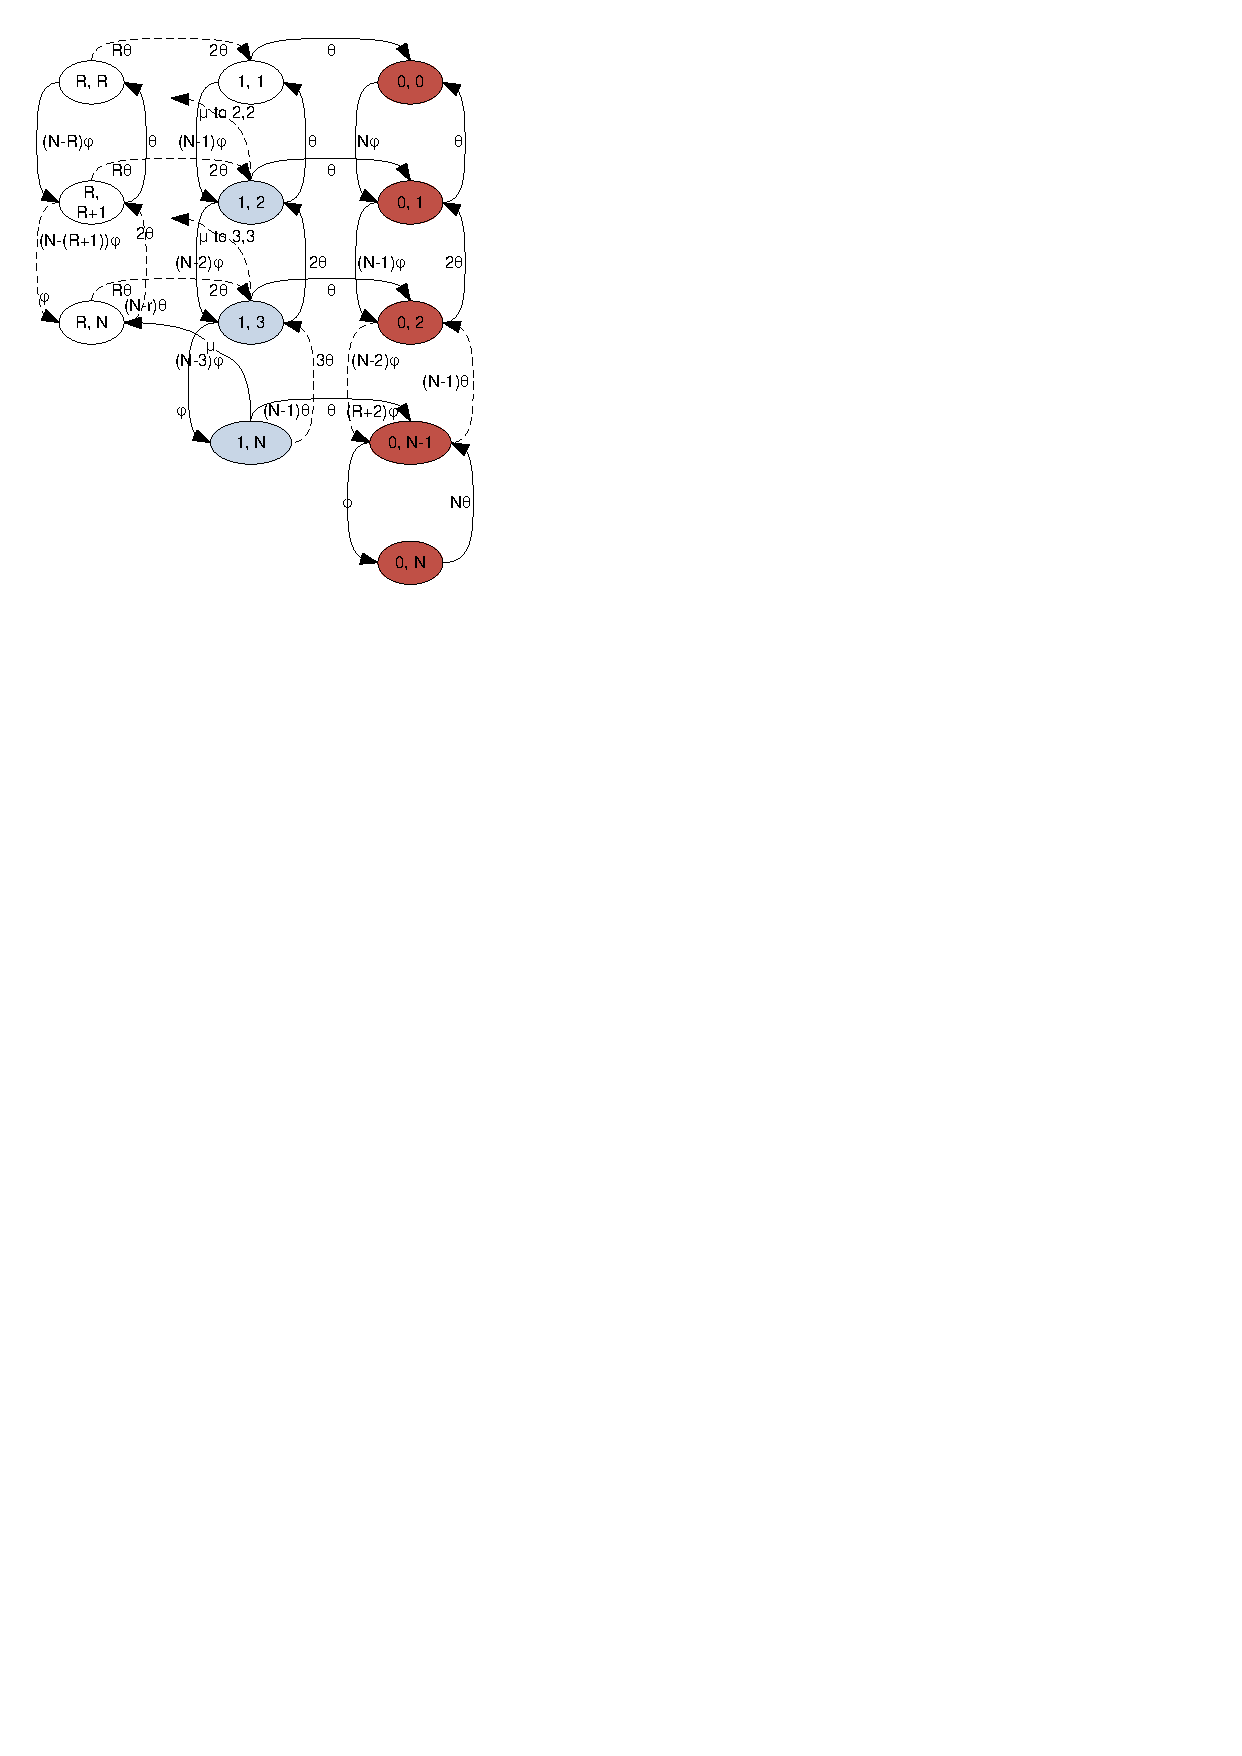
\includegraphics[clip=true, viewport=0.5cm 19.5cm 8.5cm 29.5cm, width=0.7\columnwidth]{Markov_chain_repair_compact}
 \caption{Markov chain modeling object replica number as well as network size}
 \label{fig_markov_chain}
\end{figure}

%Explain transient and absorbtion states here somewhere.

The dual parameter states can be seen in the Markov chain in Figure \ref{fig_markov_chain}. Every state is a tuple of the form \verb.(replicas,nodes).. Where $R$ is the required number of object replicas and $N$ is the maximum number of nodes in the network. It is assumed that $R$ replicas are always stored in the network, if sufficient space is available. If the number of nodes currently in the network $n$ are fewer than the required number of replicas ($n < R$), only $n$ replicas are stored. The initial states of the Markov chain are therefore all the states ($R,n$) as well as all the states ($n,n$), for $n < R$. There are therefore $N$ initial states, one for every possible network size. The initial state is the initial network size that an object is placed in.

If there are no more replicas in the network, an object cannot be repaired and the Markov chains remains in the set of states ($0,n$). These are said to be the absorbing states of the Markov chain and there exists $N - R + 1$ absorbing states in the model presented here. All other states out of which transition is possible are said to be transient states. It can be shown that if sets of transient and absorbing states exist, the system will always end up in the absorbing states \cite{grinstead1997introduction_probability}. The time to absorbtion can be calculated, which in the case of object storage means the time when no more objects exist in the network.

\subsection{State transition rates}

There are four types of state transitions possible in the Markov model presented here:
%
\begin{enumerate}
\item A node that contains a replica departs the network.
\item A node that does not contain a replica departs the network.
\item A node joins the network.
\item An object is repaired.
\end{enumerate}

%In a continous Markov chain we define delta small enough so only one event can occur at any point in time

\begin{figure}[htbp]
 \centering
 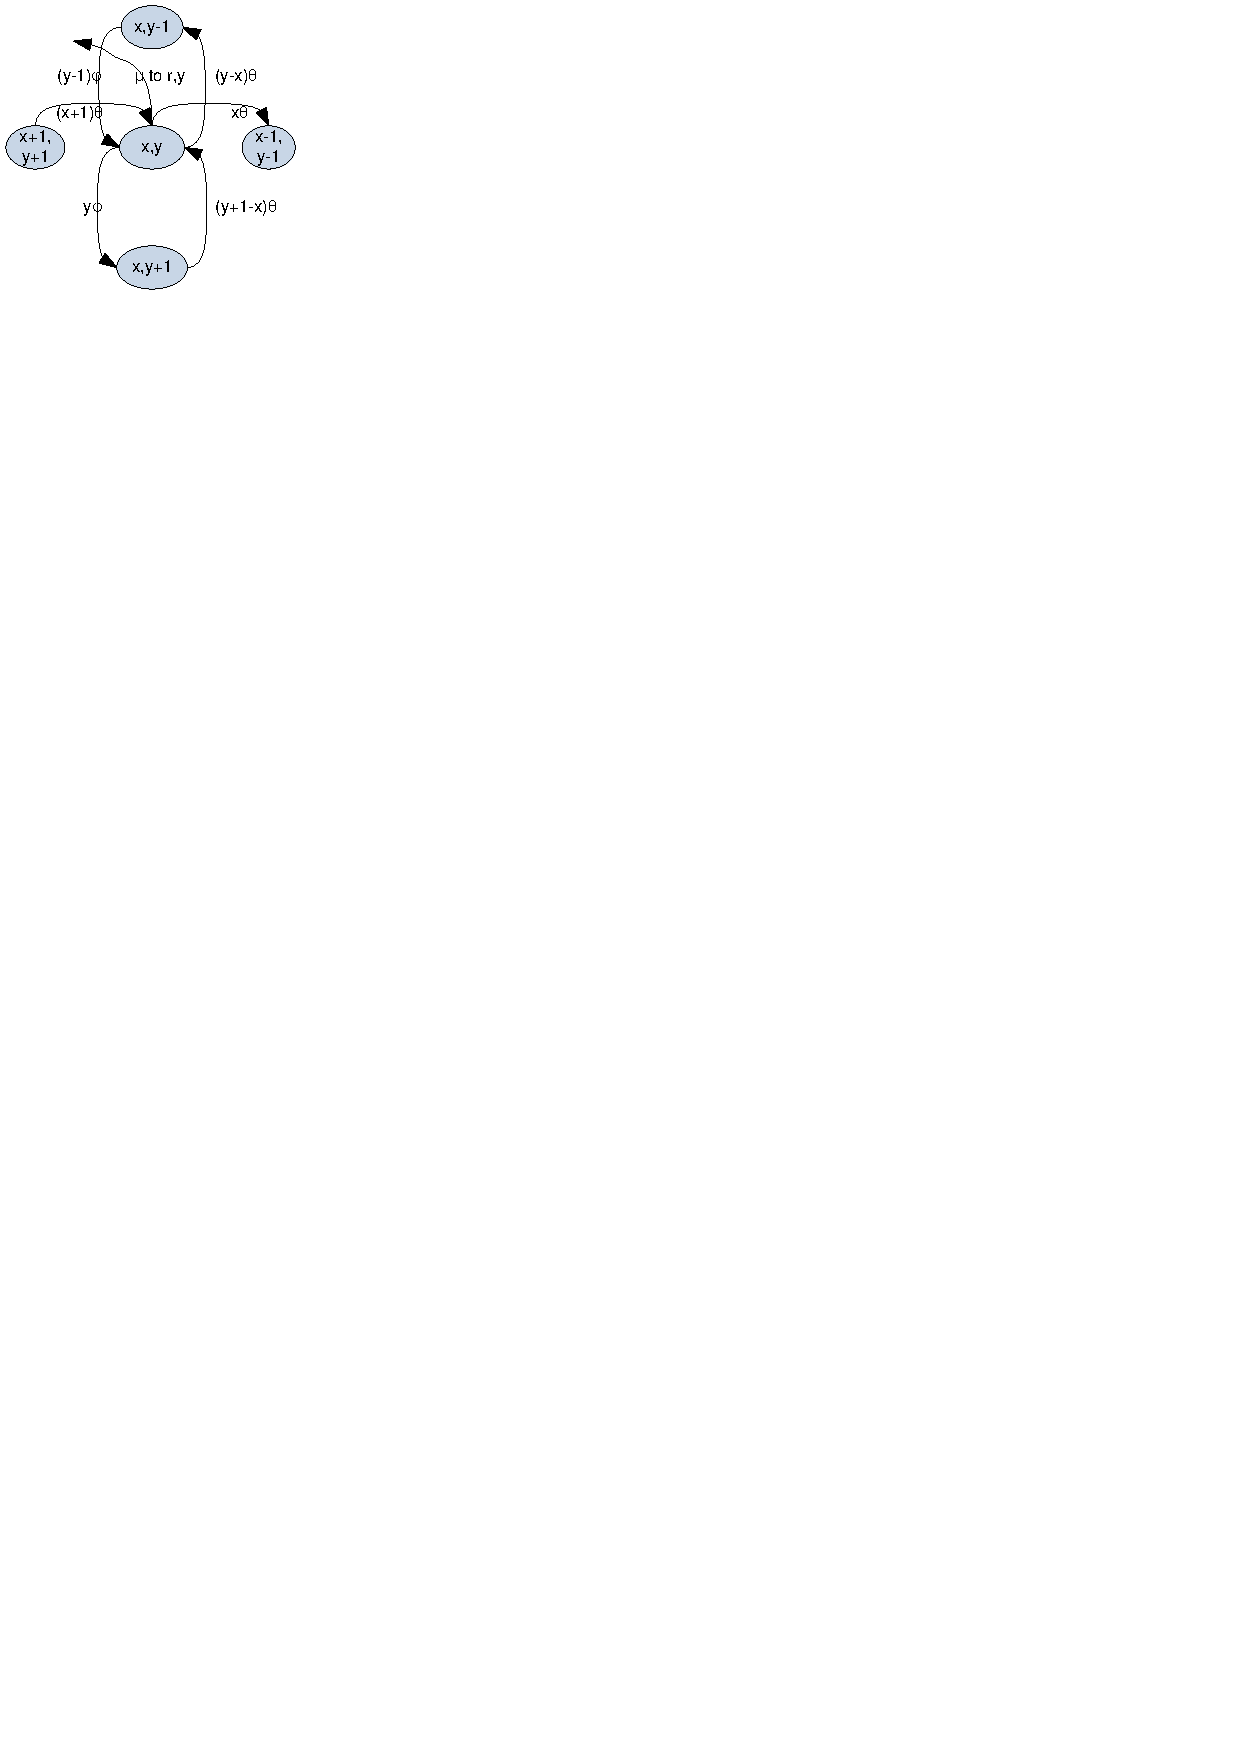
\includegraphics[clip=true, viewport=0.0cm 24.5cm 5.0cm 30cm, width=0.6\columnwidth]{Markov_example}
 \caption{Markov chain modeling object replica number as well as network size}
 \label{fig_markov_example}
\end{figure}

State transitions can be explained by the example in Figure \ref{fig_markov_example}. The figure shows all state transitions relative to the centre state ($i,k$). For the purposes of explanation, only transitions to and from the centre state are shown. Starting at state ($i+1,k+1$), where $i+1$ replicas and $k+1$ nodes are present. If a node that contains a replica departs the network, the system moves to state ($i,k$): one fewer replica and one fewer node.

If a node that does not contain a replica now departs from the network, the system moves from state ($i,k$) to ($i,k-1$): no fewer replicas and one fewer node. A node can join the network, which will have the model move from ($i,k-1$) to ($i,k$) and another node joining the network will move the system into state ($i,k+1$).

The periodic repair mechanism, introduced in Section \ref{related_work} is also present. With sufficient nodes available for a full repair, the system moves from state ($i,k$) to ($R,k$). When the network size is smaller than the required number of replicas, the system moves to state ($N,k$) instead.

For dual states, state transition rates are characterised by moving from state $i k$ to state $j l$, where $i$ is the number of replicas in the current state, $k$ the number of nodes in the current state, $j$ the number of replicas in the next state, and $l$ the number of nodes in the next state. Every state transition rate can then be expressed as a dual state transition equation.

Let $\theta$ be the departure rate of nodes under steady state. For a current state of $i$ replicas, the departure rate of nodes containing replicas from the network is $i\theta$. This transition can be expressed in terms of the dual state transition equation:
%
\begin{equation} \label{eq_rep_left}
    p(i k,j l)_{(\textrm{replica left})} = i\theta,\quad\textrm{for}\quad j = i - 1,\quad l = k - 1,
\end{equation}
%
where the next state contains one fewer replica and one fewer node than the current state.

The departure rate of nodes not containing replicas is the difference between the number of nodes currently in the network $k$ and the number of replicas currently in the network $i$. The departure rate is then $(k - i)\theta$ and the transition is given by
%
\begin{equation} \label{eq_node_left}
    p(i k,j l)_{(\textrm{node left})} = (k - i)\theta,\quad\textrm{for}\quad j = i,\quad l = k - 1,
\end{equation}
%
where the next state contains one fewer node, but the same number of replicas as the current state.

The Markov model assumes the presence of a finite sized network, with some maximum number of nodes $N$. Let $\phi$ be the arrival rate of peers under steady state. The departure rate of nodes from the network is dependant on the number of nodes in the network. Similarly, if a maximum network size is assumed, the arrival rate of nodes in the network can be modelled as a function of nodes \emph{not} in the network. This creates a symmetry between the network departure and arrival rates, which creates a ``force'' in the Markov model that pushes the network to some average network size, which is a ratio of $\theta$ to $\phi$. A stationary average network size is required to model a steady state network.

The arrival rate of nodes can thus be modelled as $(N - k)\phi$, the product of a single node arrival rate and the number of nodes not currently in the network, as given by
%
\begin{equation} \label{eq_node_arrived}
    p(i k,j l)_{(\textrm{node arrived})} = (N - k)\phi,\quad\textrm{for}\quad j = i,\quad l = k + 1,
\end{equation}
%
where the next state contains one more node, but the same number of replicas as the current state.

%Perhaps add some graphs here to show how node departure and arrival rate change with changes in network size. Show a graph or equation that will show the trend towards a single average. Perhaps use something like the rate difference to show force towards the centre.

$N$ should be chosen sufficiently large, compared to the average network size $\tilde{n}$, to ensure that the probability of the network model ever reaching $N$ is vanishingly small. What constitutes a sufficiently large maximum network size will be evident from the results presented in Section \ref{results}. This requires that the ratios of $\theta$ to $\phi$ be chosen to produce a network with an average network size much smaller than $N$.

For the network to be in steady state, the mean arrival rate of nodes must equal the mean departure rate of nodes, which gives
%
\begin{equation}
    (N - \tilde{n})\phi = \tilde{n}\theta.\label{eq_phi_theta_ratio}
\end{equation}

Making $\phi$ the subject of Equation \eqref{eq_phi_theta_ratio} gives
%
\begin{equation}
    \phi = \frac{\tilde{n}\theta}{N - \tilde{n}},\label{eq_phi}
\end{equation}
%
which provides a value for $\phi$ that will produce a network with the desired average network size $\tilde{n}$, for a given $\theta$ and $N$.

It is assumed that the repair mechanism repairs objects once every $T_{\textrm{repair}}$ time or at a rate of $\mu = 1/T_{\textrm{repair}}$, which gives
%
\begin{equation} \label{eq_repair}
    p(i k,j l)_{(\textrm{repair})} = \mu,\quad\textrm{for}\quad j = \min(R, l),\quad l = k,\quad i \neq j.
\end{equation}
%
The number of replicas in the next state is either equal to the required number of replicas or the current number of nodes, whichever one is smallest, and the number of nodes remain the same as in the current state. When no replicas are missing, no repair occurs.

No transitions other than the ones described above can occur in the presented Markov model, therefore $p(i k,j l) = 0$ for all other state transitions.

\subsection{Node departure rate}
\label{node_departure_rate}

The node departure rate $\theta$ can be calculated from the lifetime distributions of the nodes in the network. As in the related work discussed in Section \ref{related_work}, all node lifetimes are assumed to be statistically independent and exponentially distributed. The exponential distribution is characterised by the single ``rate'' parameter $\lambda$.

The departure rate of nodes correspond to the failure rate (also called the hazard rate) of the node lifetime distribution \cite{rausand2004systemreliability}. An advantage of the exponential distribution is its ``memoryless'' property, which has a constant failure rate $h = \lambda$. For nodes with exponential lifetime distributions, the node departure rate is therefore $\theta = \lambda$.

\subsection{Number of states}

The Markov model presented, possesses a large number of states. To calculate the total number of states, two cases are identified. The first case is where the number of nodes in the network is greater or equal to the required number of replicas $k \geq R$. For every possible network size in this group, there are $R$ states and $N - R + 1$ possible network sizes. From this it is evident that there are $(N - R + 1)R$ of these states.

The second case is where the number of nodes in the network is fewer than the required number of replicas. For every possible network size in this case, the number of states are equal to the number of nodes in the network, going from $R-1$ to 1.

The total number of states is the sum the two cases and given by
%
\begin{align}
       S & = R(N - R + 1) + \sum_{x=1}^{R-1} x\label{eq_states_num_init}\\
         & = R(N - R + 1) + 0.5 (R - 1) R\notag\\
         & = 0.5 R (2 N - R + 1), \quad\textrm{where}\quad N \geq R. \label{eq_states_num_ans}
\end{align}

If a small network of 500 nodes with objects each having 10 replicas is modeled, the resulting Markov chain contains 4955 states. The large number of states makes a closed form solution to the object lifetime problem intractable. Fortunately, numerical methods can be used to calculate object lifetimes for given numbers of replicas and maximum node sizes.

\subsection{Calculating object lifetimes}

Since each element in the transitional rates matrix is a rate, the sum of all the elements in a single row of the rates matrix gives the rate of moving from that state to any other state. The inverse of this rate is the expected time $t_i$ the Markov chain spends in state $i$, given by
%
\begin{equation} \label{eq_markov_rates}
    t_i = \left(\sum_{j} p_{i, j}\right)^{-1}.
\end{equation}

In a embedded Markov chain, the sum of all rows in the transitional rates matrix must equal one. This is achieved by normalising each row in the transitional rates matrix \textbf{P} to produce the normalised transitional rates matrix \textbf{\^{P}}, where each row in the matrix must satisfy
%
\begin{equation} \label{eq_markov_sum}
    \sum_{j} \hat{p}_{i, j} = 1.
\end{equation}

Using $t_i$, the expected time spent in state $i$, \textbf{\^{P}} is given by
%
\begin{equation} \label{eq_markov_normalisation}
    \hat{p}_{i, j} = p_{i, j} t_i.
\end{equation}

Object lifetime can be calculated by calculating the expected time to absorbtion of the embedded continuous time Markov chain. To do this, the normalised transitional rates matrix is partitioned into the form
%
\begin{equation} \label{matrix_partition}
    \textbf{\^{P}} = \left[\begin{array}{c|c}
                   \textbf{Q} & \textbf{R} \\
                   \hline
                   \textbf{0} & \textbf{I}
                 \end{array}\right].
\end{equation}
%
Every state transition can be considered a discrete event, which allows for the continuous time Markov chain to be embedded. This allows for theory from discrete time Markov chains to be used, with the exception that events are not equally spaced in time.

\textbf{\^{P}} is partitioned in such a way that all absorbing states are in the last rows and columns of \textbf{\^{P}}. Suppose there are $a$ absorbing states and $\tau$ transient states in the model. The matrix \textbf{Q} is then a $\tau\times\tau$ sub-matrix of \textbf{\^{P}} that contains all transient states. \textbf{I} is an $a \times a$ identity matrix, \textbf{0} is a $a\times\tau$ zero matrix and \textbf{R} (not to be confused with $R$) is a nonzero $\tau\times a$ matrix.

From \textbf{Q}, the fundamental matrix \textbf{N} may be calculated as \cite{grinstead1997introduction_probability}
%
\begin{equation} \label{eq_fundamental_mat}
    \textbf{N} = (\textbf{I} - \textbf{Q})^{-1}.
\end{equation}
%
Every element $n_{x,y}$ in the fundamental matrix \textbf{N} gives the expected number of times that the model is in the state $y$, if it started in the transient state $x$.

The expected time to absorbtion is then the product of the time spent in each state and the expected number of times a state will be entered, as given by
%
\begin{equation} \label{expected_lifetime}
    \textbf{E[L]} = \textbf{Nt},
\end{equation}
%
where \textbf{t} is the vector consisting of the times $t_i$ for all $i$.

\section{Model results}
\label{results}

For all results presented in this section, the following parameter values are used: a maximum network size of $N=120$, a required number of replicas of $R = 10$ and exponential node lifetime distributions with $\lambda = \theta = 1/1800$, which gives expected \emph{node} lifetimes of $1/\lambda = 1800$ seconds.

%Maybe explain where these values come from or why the were used.

\begin{figure}[htbp]
 \centering
 \includegraphics[clip=true, viewport=1.5cm 3.5cm 28.0cm 16.5cm, width=\columnwidth]{lifetime_av_init_groupsize}
 \caption{Surface plots of expected object lifetimes as functions of initial and average network sizes for $\mu = 1/180$ (above) and $\mu = 0$ (below).}
 \label{fig_lifetime_average_vs_initial}
\end{figure}
%
Figure \ref{fig_lifetime_average_vs_initial} shows surface plots of expected object lifetimes against initial and average network sizes for a repair rate of $\mu = 1/180$ (or $T_{\textrm{repair}}$ $10\%$ of the expected node lifetime) and no repair rate. It is evident that object lifetimes decrease greatly for average network sizes smaller than 20 nodes for the case with repair, but that average network size has no effect when repair is not used. The model presented in this chapter shows a significant decrease in expected lifetime every time the average network size is comparable to the required number of replicas, for the case with repair. The figure also shows that expected object lifetimes decrease when the initial network size is smaller than the required number of replicas. From the figure it can also be seen that initial network size has a more pronounced effect on the expected object lifetime, when no repair is used than when repair is used.

\begin{figure}[htbp]
 \centering
 \includegraphics[clip=true, viewport=2.5cm 1.0cm 27.5cm 19.15cm, width=0.8\columnwidth]{lifetime_replicas_av_groupsize}
 \caption{Surface plot of expected object lifetimes as functions of average network size and required number of replicas $R$ for $mu = 1/180$.}
 \label{fig_lifetime_average_vs_replicas}
\end{figure}
%
Figure \ref{fig_lifetime_average_vs_replicas} depicts the expected object lifetime as functions of average network size and required number of replicas $R$ for a repair rate of $\mu = 1/180$. To generate this figure, $R$ is swept from 1 to 10 to illustrate the effect that an increase in the number of replicas has on the expected node lifetime. The figure shows that an increase in $R$ leads to an exponential increase in the expected object lifetime, but that this gain is limited when the average network size is small, compared to the required number of replicas.

\begin{figure}[htbp]
 \centering
 \includegraphics[clip=true, viewport=1.0cm 6.5cm 26.5cm 20.5cm, width=0.8\columnwidth]{lifetime_av_models_compare}
 \caption{Surface plot of expected object lifetimes as functions of initial and average group sizes.}
 \label{fig_lifetime_vs_other_model}
\end{figure}

Figure \ref{fig_lifetime_vs_other_model} compares the model presented in this chapter with the model of Wu, Tian and Ng that assumes object repair \cite{replication_article}. For this figure, a repair rate of $\mu = 1/180$ and a required number of replicas of $R = 10$ were used. As shown, because the model by Wu, Tian and Ng does not take average network size into account (or initial network size for that matter) it cannot predict the object lifetimes correctly for average network sizes comparable to the required number of replicas. On the other hand, a reliability test of the model presented in this chapter is that for sufficiently large network sizes, the model converges to the model that assumes an infinite network size.

\section{Comparison with Pithos simulation}
\label{simulation}

To determine practical usability of the theoretical results presented in Section \ref{results}, a comparison was performed against the Pithos simulation \cite{Pithos_mmve_2011}. Pithos is a hierarchical distributed storage system that uses grouping to reduce latencies of store and retrieve requests, as is required by massively multi-user virtual environments (MMVEs) \cite{gilmore_p2p_mmog_state_persistency}.

The Oversim environment contains churn generators that create \emph{peers} with lifetimes sampled from an exponential distribution. A single \emph{super peer} was also created and never destroyed. Super peers allow new nodes to join the group by working with the dedicated \emph{directory server} for network bootstrapping. A single group was used, because multiple groups have different average group sizes during different simulations, which reduces the number of measurements per average group size to below statistical significance.

During a simulation run, the Pithos test application generates random objects and require these objects to be stored in the network. Every node only generated objects for a specified amount of time. This is done to limit the total number of objects present in the system to a few hundred thousand. For numbers larger than this, the simulation would run out of memory and grind to a halt. To allow simulation of the case of long lived objects, the Pithos simulation was deployed on a ``High-Memory Quadruple Extra Large Instance'' in the Amazon EC2 cloud, which contains 68.4 GB of RAM.

``Box and whiskers plots'' are used to compare the simulation data with the theoretical model. This allows for comparisons of mean values, but also shows how the data are distributed. In the box plot, the black striped whiskers show the minima and maxima of the data sets. The lower and upper bounds of the boxes show the 25th and 75th percentiles respectively. The horizontal lines in the boxes show the medians of the data, and the ``notches'' around the medians show the 5\% significance levels. The cross present in every box shows the simulation data mean and the solid line running through the boxes shows expected object lifetimes as predicted by the theoretical model.

\begin{figure}[htbp]
 \centering
 \includegraphics[clip=true, viewport=0.5cm 7.0cm 26.0cm 20.0cm, width=\columnwidth]{lifetime_simulation_model_none_100}
 \caption{Comparison of object lifetime simulation results, as a box plot, with theoretical model results for no repair, node lifetimes of $100 s$ and an average network size of 7 nodes.}
 \label{fig_lifetime_simulation_model_none_100}
\end{figure}
%
Figure \ref{fig_lifetime_simulation_model_none_100} compares the theoretical results to simulation results for the case where no repair is performed. Node have expected lifetimes of $100 s$, the number of required replicas are 10 nodes and the average network size is 7 nodes.

The expected object lifetimes as predicted by the theoretical model pass through the crosses that show the simulation data means. It can, therefore, be seen that the theoretical model matches the simulation data well for the case with no repair.

\begin{figure}[htbp]
 \centering
 \includegraphics[clip=true, viewport=1.2cm 7.0cm 26.0cm 21cm, width=\columnwidth]{lifetime_simulation_model_20_100}
 \caption{Comparison of object lifetime simulation results, as a box plot, with theoretical model results for a repair time of $20 s$, node lifetimes of $100 s$ and an average network size of 7 nodes.}
 \label{fig_lifetime_simulation_model_20_100}
\end{figure}
%
Figure \ref{fig_lifetime_simulation_model_20_100} shows simulation data and theoretical model data for the same parameters as the previous figure, but for the case with $20 s$ repair time. A significant increase in object lifetimes can be observed. Again, the expected object lifetime as predicted by the model pass through the measured object lifetime means of the simulations. For initial network sizes on the edges of measured data, the simulation data might seem to deviate from the model data. However, in these ranges, only a few hundred measurements could be made, instead of the few thousand measurements made away from the maximum and minimum initial network size. The inaccuracy in these ranges can also be seen from the wide 5\% significance levels.

One issue that was encountered when comparing simulation data to model data was the imperfect repair scheme used in simulation. In the simulation, every $T_{\textrm{repair}}$ time, a repair of all objects in the system is initiated. In simulation, there is, however, a chance that the node that was chosen to repair an object leaves the network before the repair can complete. This reduces the effectiveness of the repair mechanism, reducing the effective repair rate. The percentage repair successes was measured during simulation and found to be $70 \%$. All repair rates in the simulation were adjusted with this number, which successfully aligned the simulation data means with the model data means.

\section{Conclusion}
\label{conclusion}

A Markov chain that takes network size into account when predicting object lifetimes was presented. Results show that when the average network size is comparable to the required number of replicas, object lifetimes are significantly decreased. The theoretical model was shown to be equivalent to a model that ignores network size, when the average network size is large, compared to the required number of replicas. The model was also shown to compare well to simulation, with values being nearly equal.

We show how to reliably predict expected object lifetimes. When it is known that the average network size is comparable to the required number of replicas, the network size should be taken into account when modelling object lifetimes in a situation with repair. The theoretical model presented here allows for the design of a distributed storage system when the various average network sizes and node lifetime distributions are known.

Future work includes comparing object lifetimes using replication, with object lifetimes using erasure coding as redundancy technique. Modelling object lifetimes using heavy-tailed node lifetime distributions, such as the Pareto distribution, is also required. The variable failure rate of the Pareto distribution complicates modelling it as a Markov chain.

%\chapter{Pithos verification}
    \label{chp:VERIFICATION}


    \section{Metrics}

    \section{Theoretical results}

    \section{Comparison between theoretical and simulation results}

        \subsection{Overhead}
        \subsection{Fairness}
        \subsection{Reliability}
        \subsection{Responsiveness}
\chapter{Conclusions and Recommendations}
\label{chp:CONC}

This work focussed on developing a state management architecture for P2P MMVEs. In order to do this, an understanding was required of P2P networks, MMVEs and what the main challenges of P2P MMVEs are.  It was found that state management and persistency is used by the consistency architecture and, therefore, that the consistency architecture implicitly specifies the storage requirements.

After having identified the requirements of a state management and persistency architecture, related work was reviewed and compared against the identified requirements. This allowed us to identify areas where improvements might be made.

The design of Pithos was presented in order to satisfy all identified requirements, presenting every aspect of Pithos in terms of the requirement identified. The Pithos use case was reviewed and presented as a distributed storage system and the mechanisms to implement the use cases were discussed.

With the conceptual design finalised, the implementation specifics were reviewed. Pithos has been implemented as an Oversim simulation that allows for large scale simulations. Some implementation issues that were reviewed were maintaining group consistency as well as persistency in group storage. An evaluation was performed in order to verify that Pithos satisfies all the requirements originally identified.

When Pithos was evaluated for various churn levels and repair rates, it was seen that many factors influence reliability. The factors influencing reliability were found to be directly related to expected object lifetime. A Markov chain model was developed to allow for the prediction of expected object lifetimes. It was found that the literature reviewed assumed an infinite network size and does not take limited network sizes into account. Comparing our model with simulation results, it was found that finite group sizes does affect object lifetimes when the average group size is small, compared to the required number of replicas.

\section{State consistency}

The generic consistency model developed provides a framework for the design and development of MMVEs in general. Because many aspects of the generic consistency model are trivial in C/S models, the model is perhaps more applicable to a P2P MMVE

\section{State management}

\section{Pithos}


\section{Further work}
\label{further_work}


%==== Appendices ====================================================
\appendix
\appendixpage\relax

\chapter{Ensuring group consistency in Pithos}
\label{chp:GROUP_INCONSISTENCY}

This appendix described, in chronological order, the steps taken to ensure group consistency. It provides initial findings, discusses the reasons for inconsistency and introduces the proposed solutions.

\section{Initial approach}
The initial approach to achieve group consistency was to have every peer inform all other peers when it was moving from one group to another. If a peer is removed from the network due to churn, another peer has to discover that the peer has left, which is done with timeouts. If a request times out, the peer making the request informs the group of the peer that left.

\begin{figure}[htbp]
 \centering
 \includegraphics[clip=true, viewport=0mm 0mm 460mm 212mm, width=\columnwidth]{gc_first}
 \caption{Group consistency before any improvements}
 \label{fig_gc_first}
\end{figure}
%
Figure \ref{fig_gc_first} shows an enlarged view of the perceived group size of every node in the group for the initial group consistency scheme. The lines running across the graph is due to nodes leaving the network and joining again at a later time.

From approximately 2925 s, a new peer joins the group and reports the group size as eight, when all other peers report the group size as seven. Multiple variations of these inconsistencies occurred during testing. A primary source of inconsistencies was the fact that it takes time to inform all group peers of a peer that left and that it takes time to inform all group peers of a peer that joined.

Issues also occurred because of how newly stored objects are handled. When a new peer joins the group, it starts to generate objects. The group super peer sends a joining peer a list of group peers. After this occurs, the group peers are informed of the new peer. A peer joining a group can immediately start to store objects at the request of other peers. This can happen before some peers are aware of the joining peer. The unaware peers will then get a message saying that an object has been stored on the new peer, before they are aware of the new peer. The solution was to assume that an object was generated by a valid peer and to add any unknown peer information contained in an object add message to the peers list in the group ledger.

Group inconsistency can arise because there might be some latent object add messages still enroute to peers, after the peer has already left the network and informed other peers of its leaving. This means that a peer has already left, but after it informed the group peers of its leaving and all group peers have removed the peer from memory, the group peers receive a message for an object that is supposedly now stored on the peer that just left. The mechanism mentioned above is initiated and the, now unknown, peer is again added to the peer list.

Many transient group states that led to inconsistencies were solved by the super peer storing the information of the last peer that left and the last peer that joined. Every time a new peer joins, the super peer informs the joining peer of the last peer that left. This allows the joining peer to ignore any latent object add messages received from the leaving peer. Any messages received from the last peer that left are ignored. This prevents latent messages from peers that left to affect the group view of peers.

\section{Peer starvation problem}
\begin{figure}[htbp]
 \centering
 \includegraphics[clip=true, viewport=0mm 0mm 455mm 212mm, width=\columnwidth]{gc_middle}
 \caption{Group consistency with starvation}
 \label{fig_gc_middle}
\end{figure}
%
The mentioned improvements created the issue shown in Figure \ref{fig_gc_middle}, where a peer will believe that another peer has left. The group will be informed of the peer that supposedly left, but is actually still present in the group. Because all peers will now ignore messages from the peer that supposedly left, including the super peer, all requests sent by the peer that supposedly left will be ignored. The requests will then timeout on the ignored peer and the ignored peer will remove all group peers. This isolates the peer and prevents any requests from being serviced.

The starvation was caused by peers not responding to requests. A scenario could occur where a peer did not contain a requested object or where the network bandwidth was limited, which prevented a response from arriving at a peer before the request timeout expired. In either of these two situation, the peer making the request was under the impression that the target peer had left the network. It then informed all other peers of this.

The solution to this issue was to adjust the timeout as a function of the available network bandwidth and to make sure every node always responded to a request, whether as a success or failure. Functionality was also added to the super peer to check whether a peer that was reported as having left, actually did leave the network.

Other issues were caused when group migration was enabled. A node might leave a group to move to another, but as the node leaves some peer that has not been informed of the peer leaving would make a request form the leaving peer. The leaving peer would respond to that request, which would have the requesting peer add the peer back into the group. This could cause the situation where peers existed in multiple groups.

The solution to this was to include the group membership information in every request message. A peer's membership can be uniquely identified by the IP address and port of the group's super peer. If a peer receives a message with a different group address than its own, it ensures that that peer is not part of its group.

This also solved the case where Peer A requested an object from Peer B, just as Peer B was leaving the group. Peer B will already be in its new group when receiving the request from Peer A. Peer B will see that the request originated from outside its group, so will not add the new peer to its group. If it contains the requested object, it will however still respond with the object. When Peer A receives the object, it will detect that it was sent from another group and remove Peer B from its group ledger. In this way, the request was successfully handled and group consistency is maintained.

\section{Final solution}
\begin{figure}[htbp]
 \centering
 \includegraphics[clip=true, viewport=12mm 35mm 275mm 165mm, width=\columnwidth]{gc_final_png}
 \caption{Group consistency after all improvements}
 \label{fig_gc_final_app}
\end{figure}
%
Figure \ref{fig_gc_final_app} shows the group consistency after all improvements were added for a larger group than the previous two. Even with the larger group, complete consistency is achieved.

When object lifetime was tested, all requests were stopped after a certain period of time to speed up the simulation. This created an issue where group peers did not become aware of peers leaving the group, because no peers sent requests that could timeout. This prompted the addition of keep-alive messages.

Regular keep alive messages are sent to peers. If a peer does not respond to the message, that peer is removed from the group. The time between keep alive messages can be adjusted as a function of network churn. In order to reduce the load on the super peer, each peer randomly chooses a target peer and sends a keep-alive message, as explained in Section \ref{leave_design}.


%==== Bibliography acro's & Index ===================================
%\backmatter

%\newpage
%\IEEEtriggeratref{43} %Balance the bibliography
\bibliographystyle{IEEEannot}
\bibliography{../BibTeX/P2P_MMOG}

\end{document}
